\documentclass[10pt]{article}

% -----------------------------------------------------------------------------
% Single-column academic technical report.
% -----------------------------------------------------------------------------

\usepackage[a4paper,top=1.85cm,bottom=1.85cm,left=1.9cm,right=1.9cm]{geometry}
\usepackage[T1]{fontenc}
\usepackage[utf8]{inputenc}
% \usepackage{newtxtext,newtxmath}
\usepackage{lmodern}
\usepackage[expansion=false]{microtype}
\usepackage{amsmath,bm}
\usepackage{graphicx}
\usepackage{booktabs}
\usepackage{array}
\usepackage{multirow}
\usepackage{enumitem}
\usepackage[font=footnotesize,labelfont=bf,labelsep=colon]{caption}
\usepackage{subcaption}
\usepackage{float}
\usepackage{tikz}
\usepackage{algorithm}
\usepackage{algpseudocode}
\usepackage{xcolor}
\usepackage{titlesec}
\usepackage{titletoc}
\usepackage{fancyhdr}
\usepackage{url}
\usepackage{hyperref}
\usepackage{balance}
\usetikzlibrary{arrows.meta,positioning,shapes.geometric,calc,fit,backgrounds}

\definecolor{accessblue}{RGB}{0,144,181}
\definecolor{accesscyan}{RGB}{0,169,206}
\definecolor{lightbluebox}{RGB}{232,247,252}
\definecolor{lightorangebox}{RGB}{250,239,225}
\definecolor{lightgreenbox}{RGB}{235,247,235}
\definecolor{lightgraybox}{RGB}{244,244,244}

\hypersetup{
    colorlinks=true,
    linkcolor=accessblue,
    citecolor=accessblue,
    urlcolor=accessblue,
    pdftitle={Autonomous Differential-Drive Robot for Garage EV Charging: A Dynamic Visual SLAM Approach with RL-Augmented Precision Docking},
    pdfauthor={Ammar Daher & Naya Yousef & Salman Daher & Mohammad Saoud}
}

\setlength{\parindent}{1em}
\setlength{\parskip}{1.2pt}
\setlength{\floatsep}{6pt plus 1pt minus 1pt}
\setlength{\textfloatsep}{8pt plus 1pt minus 2pt}
\setlength{\intextsep}{6pt plus 1pt minus 1pt}
\setlength{\abovedisplayskip}{6pt}
\setlength{\belowdisplayskip}{6pt}
\setlength{\abovedisplayshortskip}{4pt}
\setlength{\belowdisplayshortskip}{4pt}
\setlength{\jot}{2pt}
\setlength{\emergencystretch}{1.3em}
\setlist[itemize]{leftmargin=1.15em,topsep=2pt,itemsep=1pt,parsep=0pt}
\setlist[enumerate]{leftmargin=1.25em,topsep=2pt,itemsep=1pt,parsep=0pt}

\renewcommand{\thesection}{\Roman{section}}
\renewcommand{\thesubsection}{\Alph{subsection}}
\renewcommand{\thesubsubsection}{\arabic{subsubsection})}

\titleformat{\section}
  {\color{accessblue}\bfseries\Large}
  {\thesection.}{0.6em}{}
\titlespacing*{\section}{0pt}{1.4ex plus .2ex minus .1ex}{0.55ex}
\titleformat{\subsection}
  {\bfseries\large}
  {}{0pt}{}
\titlespacing*{\subsection}{0pt}{1.0ex plus .15ex minus .1ex}{0.35ex}
\titleformat{\subsubsection}
  {\bfseries\itshape}
  {}{0pt}{}
\titlespacing*{\subsubsection}{0pt}{0.7ex}{0.2ex}

% Only top-level sections carry Roman numerals. Subsection entries retain their
% hierarchy in the contents page but intentionally omit letters and numbers.
\titlecontents{section}
  [0pt]{\vspace{0.35em}\color{accessblue}\bfseries}
  {\contentslabel{2.2em}}{}
  {\titlerule*[0.45pc]{.}\contentspage}
\titlecontents{subsection}
  [1.65em]{\small}
  {}{}
  {\titlerule*[0.45pc]{.}\contentspage}
\titlecontents{subsubsection}
  [3.25em]{\footnotesize}
  {}{}
  {\titlerule*[0.45pc]{.}\contentspage}

\captionsetup[figure]{name=FIGURE,justification=centering}
\captionsetup[table]{name=TABLE,justification=centering}
\renewcommand{\tablename}{TABLE}
\renewcommand{\figurename}{FIGURE}

\pagestyle{fancy}
\fancyhf{}

\fancyhead[R]{\footnotesize \textit{Autonomous Differential-Drive Robot for Garage EV Charging}}
%\fancyfoot[L]{\footnotesize TECHNICAL REPORT, MAY 2026}
\fancyfoot[R]{\footnotesize \thepage}
\renewcommand{\headrulewidth}{0.25pt}
\renewcommand{\footrulewidth}{0pt}

\newcommand{\R}{\mathbb{R}}
\newcommand{\SE}{\mathrm{SE}}
\newcommand{\SO}{\mathrm{SO}}
\newcommand{\T}{\mathbf{T}}
\newcommand{\Rmat}{\mathbf{R}}
\newcommand{\tvec}{\mathbf{t}}
\newcommand{\q}{\mathbf{q}}
\newcommand{\qd}{\dot{\mathbf{q}}}
\newcommand{\pc}{\mathbf{p}_{c}}
\newcommand{\pg}{\mathbf{p}_{g}}
\newcommand{\pv}{\mathbf{p}_{v}}
\newcommand{\pe}{\mathbf{p}_{e}}
\newcommand{\fc}{\mathbf{f}_{c}}
\newcommand{\fe}{\mathbf{f}_{e}}
\newcommand{\fid}{\mathbf{f}_{\mathrm{id}}}
\newcommand{\cmd}{\mathbf{u}_{\mathrm{cmd}}}
\newcommand{\eori}{e_{\psi}}

\newcommand{\reportplaceholder}[2]{%
  \fbox{%
    \begin{minipage}[c][0.115\textheight][c]{0.84\textwidth}
      \centering\footnotesize
      \textbf{IMAGE PLACEHOLDER}\\[-0.05em]
      \emph{#1}\\[0.20em]
      \parbox{0.94\linewidth}{\centering #2}
    \end{minipage}%
  }%
}

\begin{document}

\noindent\begin{minipage}{\textwidth}
\centering\LARGE\bfseries Autonomous \textbf{Differential-Drive Robot for Garage EV Charging: Dynamic Visual SLAM approach with RL-Augmented Precision Docking}\par
\end{minipage}\vspace{0.35em}

\begin{center}
{\large Ammar Daher, Mohammad Saoud, Naya Yousef, Salman Daher}\\\vspace{0.15em}

{\normalsize Department of Robotics and Intelligent Systems Engineering, Manara University, Syria}\\[0.2em]
{\normalsize Supervisor: Dr. Mothanna Alkubeily}
\end{center}\vspace{0.5em}

\noindent\rule{\textwidth}{0.35pt}\vspace{0.6em}

\noindent \textcolor{accessblue}{\bfseries ABSTRACT}\quad
Autonomous plug-in charging for electric vehicles is difficult because it requires accurate navigation, local pose estimation, and safe physical interaction during connector insertion. The charging process comprises four main phases: mobile-base approach, socket localization, plug-socket alignment, and contact-aware insertion. Small deviations in the robot trajectory, connector orientation, or applied contact force can lead to insertion failure, excessive mechanical stress, or unsafe interaction with the socket.

This project introduces a laboratory-safe robotic framework for autonomous conductive charging. The platform combines a differential mobile base, a base-mounted Intel RealSense D435i camera for dynamic visual SLAM, a 3-DoF arm, and a Logitech C920 eye-in-hand camera (1080p RGB) for local socket observation. The system is implemented in ROS~2 and evaluated in Isaac Sim and Isaac Lab. The dynamic visual SLAM stage provides the mobile robot with a stable map and an approach pose near the target socket, while the eye-in-hand camera supports local plug-socket pose estimation during the final alignment phase.

The proposed framework combines perception, navigation, reinforcement learning, and contact-aware control to execute the simplified plug-in charging task. A reinforcement-learning policy trained with Proximal Policy Optimization (PPO) refines the final alignment and insertion motion, while safety checks and force-aware constraints reduce excessive contact during interaction. The report defines and evaluates this complete pipeline for the laboratory plug-in socket experiment.
\vspace{0.5em}




\noindent \textcolor{accessblue}{\bfseries INDEX TERMS}\quad Autonomous charging, mobile manipulation, contact-rich connector insertion, dynamic visual SLAM, reinforcement learning, Isaac Lab, ROS~2, eye-in-hand perception.\vspace{0.85em}

\tableofcontents
\clearpage
\listoffigures
\clearpage
\listoftables
\clearpage
\section{Introduction}

Research on electric vehicles (EVs) has grown rapidly in recent years, and robotic technology is being developed to support this growth. One important direction is the automation of EV charging, where robotic and electronic systems plug and unplug the charging connector automatically. In this process, the connector must be inserted into the vehicle charging socket with proper alignment.

Automated charging stations are therefore not only an energy-transfer problem but also a robotic manipulation problem: the charging connector must be guided toward the socket, aligned with the inlet, and inserted through a controlled motion. Previous studies on EV charging connectors have shown that the plugging and unplugging process strongly affects the safety and efficiency of charging, and that the motion profile during insertion is important for designing reliable robotic charging systems. Whereas that prior work characterizes the connection through force and torque, this project is motivated by the smoothness and safety of the plug-in motion, expressed through acceleration and jerk. Acceleration describes how quickly the connector velocity changes, and jerk is the rate of change of acceleration. Both quantities indicate motion smoothness: keeping them bounded reduces abrupt movements and improves the safety of insertion.

At the same time, the robot must operate in an environment that may contain moving objects. Simultaneous localization and mapping (SLAM) is an established research field in robotics, but many SLAM methods rely on the static-world assumption. This assumption limits their use in real-world environments that are dynamic, unstructured, and only partially known. Dynamic visual SLAM addresses this limitation by allowing the robot to build a map while accounting for moving objects in the scene. A mobile charging robot needs this capability, since it must navigate toward the charging area, maintain a stable representation of the environment, and avoid treating dynamic objects as reliable static landmarks.

This project studies a laboratory-safe version of autonomous plug-in charging using a differential mobile base, a base-mounted RGB-D camera for dynamic visual SLAM, a 3-DoF robotic arm, and an eye-in-hand RGB camera for local socket observation. The mobile base uses the SLAM stage to approach the target socket and maintain a map of the surrounding environment. The arm then performs the local alignment and insertion task. During this final phase, the end-effector mounting plane is kept parallel to the mobile-base ($x_b$-$y_b$) plane, which simplifies the plug-socket alignment problem and makes the experiment suitable for a controlled laboratory setup.

The main objective of this work is to define and evaluate a robotic pipeline for simplified plug-in charging. The pipeline is organized into six implementation stages: mobile-base navigation, dynamic visual SLAM, local socket observation, plug-socket pose estimation, final alignment, and insertion. The study also defines the task phases, observation and action spaces, safety limits, reward function, and evaluation metrics. Motion smoothness and safety remain a guiding concern, with acceleration and jerk taken as indicators of how smooth the insertion motion is. A successful system should therefore not only reach the socket but also do so through a stable, smooth, and safe motion.

\clearpage
\section{Objectives}

The primary aim of this thesis is to design, implement, and validate a complete robotic pipeline for autonomous conductive EV charging in a controlled laboratory environment. The objectives are structured to address each major subsystem in sequence, from the physical platform through to full mission integration.

The first objective is to design and fabricate a compact differential-drive mobile robot platform capable of operating safely inside a structured indoor space. This encompasses the mechanical design of the mobile base, a three-degree-of-freedom robotic arm, and a passive compliant wrist that absorbs residual misalignment during plug-socket contact. The platform must also be modelled as a digital twin inside Isaac Sim, with kinematics and joint dynamics validated against the physical hardware before deployment.

The second objective is to develop and integrate a dynamic visual SLAM pipeline that maintains stable robot localization and a consistent static map of the environment even when moving objects are present in the scene. The pipeline must classify and suppress dynamic features so that they do not contaminate the map or corrupt the pose estimates that the navigation module relies on during approach.

The third objective is to implement socket detection and local pose estimation from the eye-in-hand RGB camera using a category-level keypoint-based object pose estimator. The estimated socket pose must be accurate enough, across a range of standoff distances, yaw angles, and lighting conditions, to bring the plug tip within the verified capture range of the fine-alignment controller without manual positioning.

The fourth objective is to implement autonomous point-to-point navigation from a known base station to the target parking bay using the ROS~2 Navigation~2 stack with an MPPI local controller, operating on the costmap generated from the SLAM-derived voxel map. Navigation must succeed without collision and without operator intervention across all tested starting poses and obstacle configurations.

The fifth objective is to design and train a reinforcement-learning insertion policy using Proximal Policy Optimization in Isaac Lab that refines final plug-socket alignment and executes the contact phase of insertion. The policy must improve terminal alignment accuracy over the deterministic inverse-kinematics baseline and must produce smooth, bounded motion quantified through jerk and acceleration metrics throughout the insertion trajectory.

The sixth objective is to evaluate the sim-to-real transfer of the trained insertion policy on the physical robot through a structured hardware protocol spanning at least thirty trials across centred, left-offset, and right-offset initial conditions, and to identify the dominant failure modes that constrain physical performance.

The seventh and final objective is to integrate all subsystems — dynamic SLAM, global navigation, socket detection, base refinement, arm control, and RL insertion — into a single state-machine-governed pipeline and to demonstrate complete autonomous charging missions in the laboratory from an arbitrary start pose to confirmed plug seating, without manual intervention at any stage.

\section{Related Works}

Hanai \textit{et al.}, working on robotic wrapping and deformable manipulation, proposed a framework that combines imitation learning and reinforcement learning. Their method uses demonstrations to obtain approximate tool-center-point trajectories and then uses RL to tune force-control parameters. The shared learning logic, rather than the wrapping task itself, is what carries over to our work: a nominal trajectory constrains the search space while RL corrects the contact behavior. Their training procedure also separates simulation training from real-world force adaptation, which parallels our sim-to-real plan, in which Isaac Sim is the simulator \cite{hanai2025wrapping}.

Wang \textit{et al.} studied complex contact-rich insertion and presented an adaptive imitation learning framework that treats insertion as a nonlinear, low-clearance operation with phase-dependent force requirements. The term ``contact-rich insertion'' is established in the robotics literature for tasks where contact is expected and must be regulated rather than avoided. They explain why pure imitation learning is insufficient when force profiles are difficult to acquire, and why pure RL can be unsafe, since random exploration may cause excessive collisions. Their solution combines a trajectory-level skill policy with a low-level force-learning policy and introduces dynamical movement primitives to generalize trajectories between related insertion tasks \cite{wang2022adaptive}. This supports a key design choice in our project: rather than inserting the plug with blind random RL, the plug follows a structured nominal path and RL is used mainly for corrections and contact adaptation.

Saputra \textit{et al.} examined EV charging connector interaction, characterizing plugging and unplugging of a Type~2 AC EV connector using force/torque measurements. Their experiments with human operators showed that plugging requires a higher impulse than unplugging and that the force and torque profiles vary over time. They also modeled these profiles using polynomial, Fourier, and Gaussian fitting, with the Gaussian model giving the most accurate fit \cite{saputra2025evft}. These results motivate our reward and safety design. Even though our laboratory socket is simplified, the plug-in stage should still be treated as a force-sensitive operation rather than a purely geometric motion.

For robotic charging systems, previous works have used computer vision, force sensing, and mobile manipulation to localize the charging inlet and perform connector insertion \cite{miseikis2017charging,rakhmatulin2024pose,zhou2021plug,guo2021visionforce,chablat2022charging}. Such methods are highly relevant because the charging task can be modeled as a peg-in-hole insertion problem with perception uncertainty. Many approaches focus on perception or local alignment, and fewer studies connect global mobile navigation, dynamic-scene SLAM, and contact-rich arm insertion in a single prototype pipeline. This is the gap the present project targets, combining dynamic visual SLAM for the approach with reinforcement learning for the local alignment and insertion.


\section{System Design}
\label{sec:system_design}

\subsection{Task}
\label{sec:task}

The task starts with a mapping run inside the garage. Before charging requests are handled, the robot drives through the accessible lanes while the base-mounted RGB-D camera records depth images, and dynamic visual SLAM estimates the camera pose during this scan. From the depth images and poses, nvblox builds a 3-D voxel map of the garage and produces a 2-D costmap for navigation \cite{millane2024nvblox,nvidia_nvblox}. The map represents the fixed parts of the garage, such as walls, pillars, lane boundaries, and the base station, and serves as the reference map during later charging runs.

At the start of each charging run, the robot sits at the base station, a fixed and known location in the garage map. The robot is connected there to charge its own battery, so its initial pose is known before it moves. When a vehicle enters the garage, the system receives its parking-bay location, which becomes the navigation goal. The goal is the parking area, not the charging socket, because the socket position is not known until the robot reaches the vehicle.

The global navigation stage moves the robot from the base station to the requested parking bay. A cost-aware A* planner in the ROS~2 Navigation 2 stack (Nav2) searches the costmap and creates a collision-free route \cite{nav2_smac}. Dynamic visual SLAM supplies the current base pose while the robot follows this route. For local control, Nav2 uses a Model Predictive Path Integral (MPPI) controller with the differential-drive motion model: at each control step it generates and scores short candidate trajectories, then sends the next linear and angular velocity command \cite{nav2_mppi}. This navigation stack is first validated in Isaac Sim with the same base and sensor arrangement, then deployed on the physical robot through the ROS~2 command chain.

When the robot reaches the parking bay, it stops following the global route and begins the socket-search stage. A CenterPose detector finds the charging socket in the RGB image: it detects the object and its image keypoints, then estimates the pose of the trained socket class \cite{lin2022centerpose}. This RGB pose is combined with the depth image and the calibrated camera-to-base transform to obtain a coarse socket location in the base frame. The mobile base then makes small position and heading corrections until the socket lies inside the calibrated reachable workspace of the arm, the condition required before the arm begins the final alignment task.

After this base adjustment, the eye-in-hand camera provides the close-range view needed for the fine plug-socket estimate. The RL policy then corrects the remaining alignment error and performs the insertion motion. The policy is trained offline in Isaac Lab, with socket pose, base stopping error, contact conditions, and sensor effects varied during training \cite{nvidia_isaaclab,haarnoja2018sac}. No online RL training is performed on the physical arm; the real robot runs the saved policy for inference, together with the predefined safety limits.

\begin{figure}[!htbp]
\centering
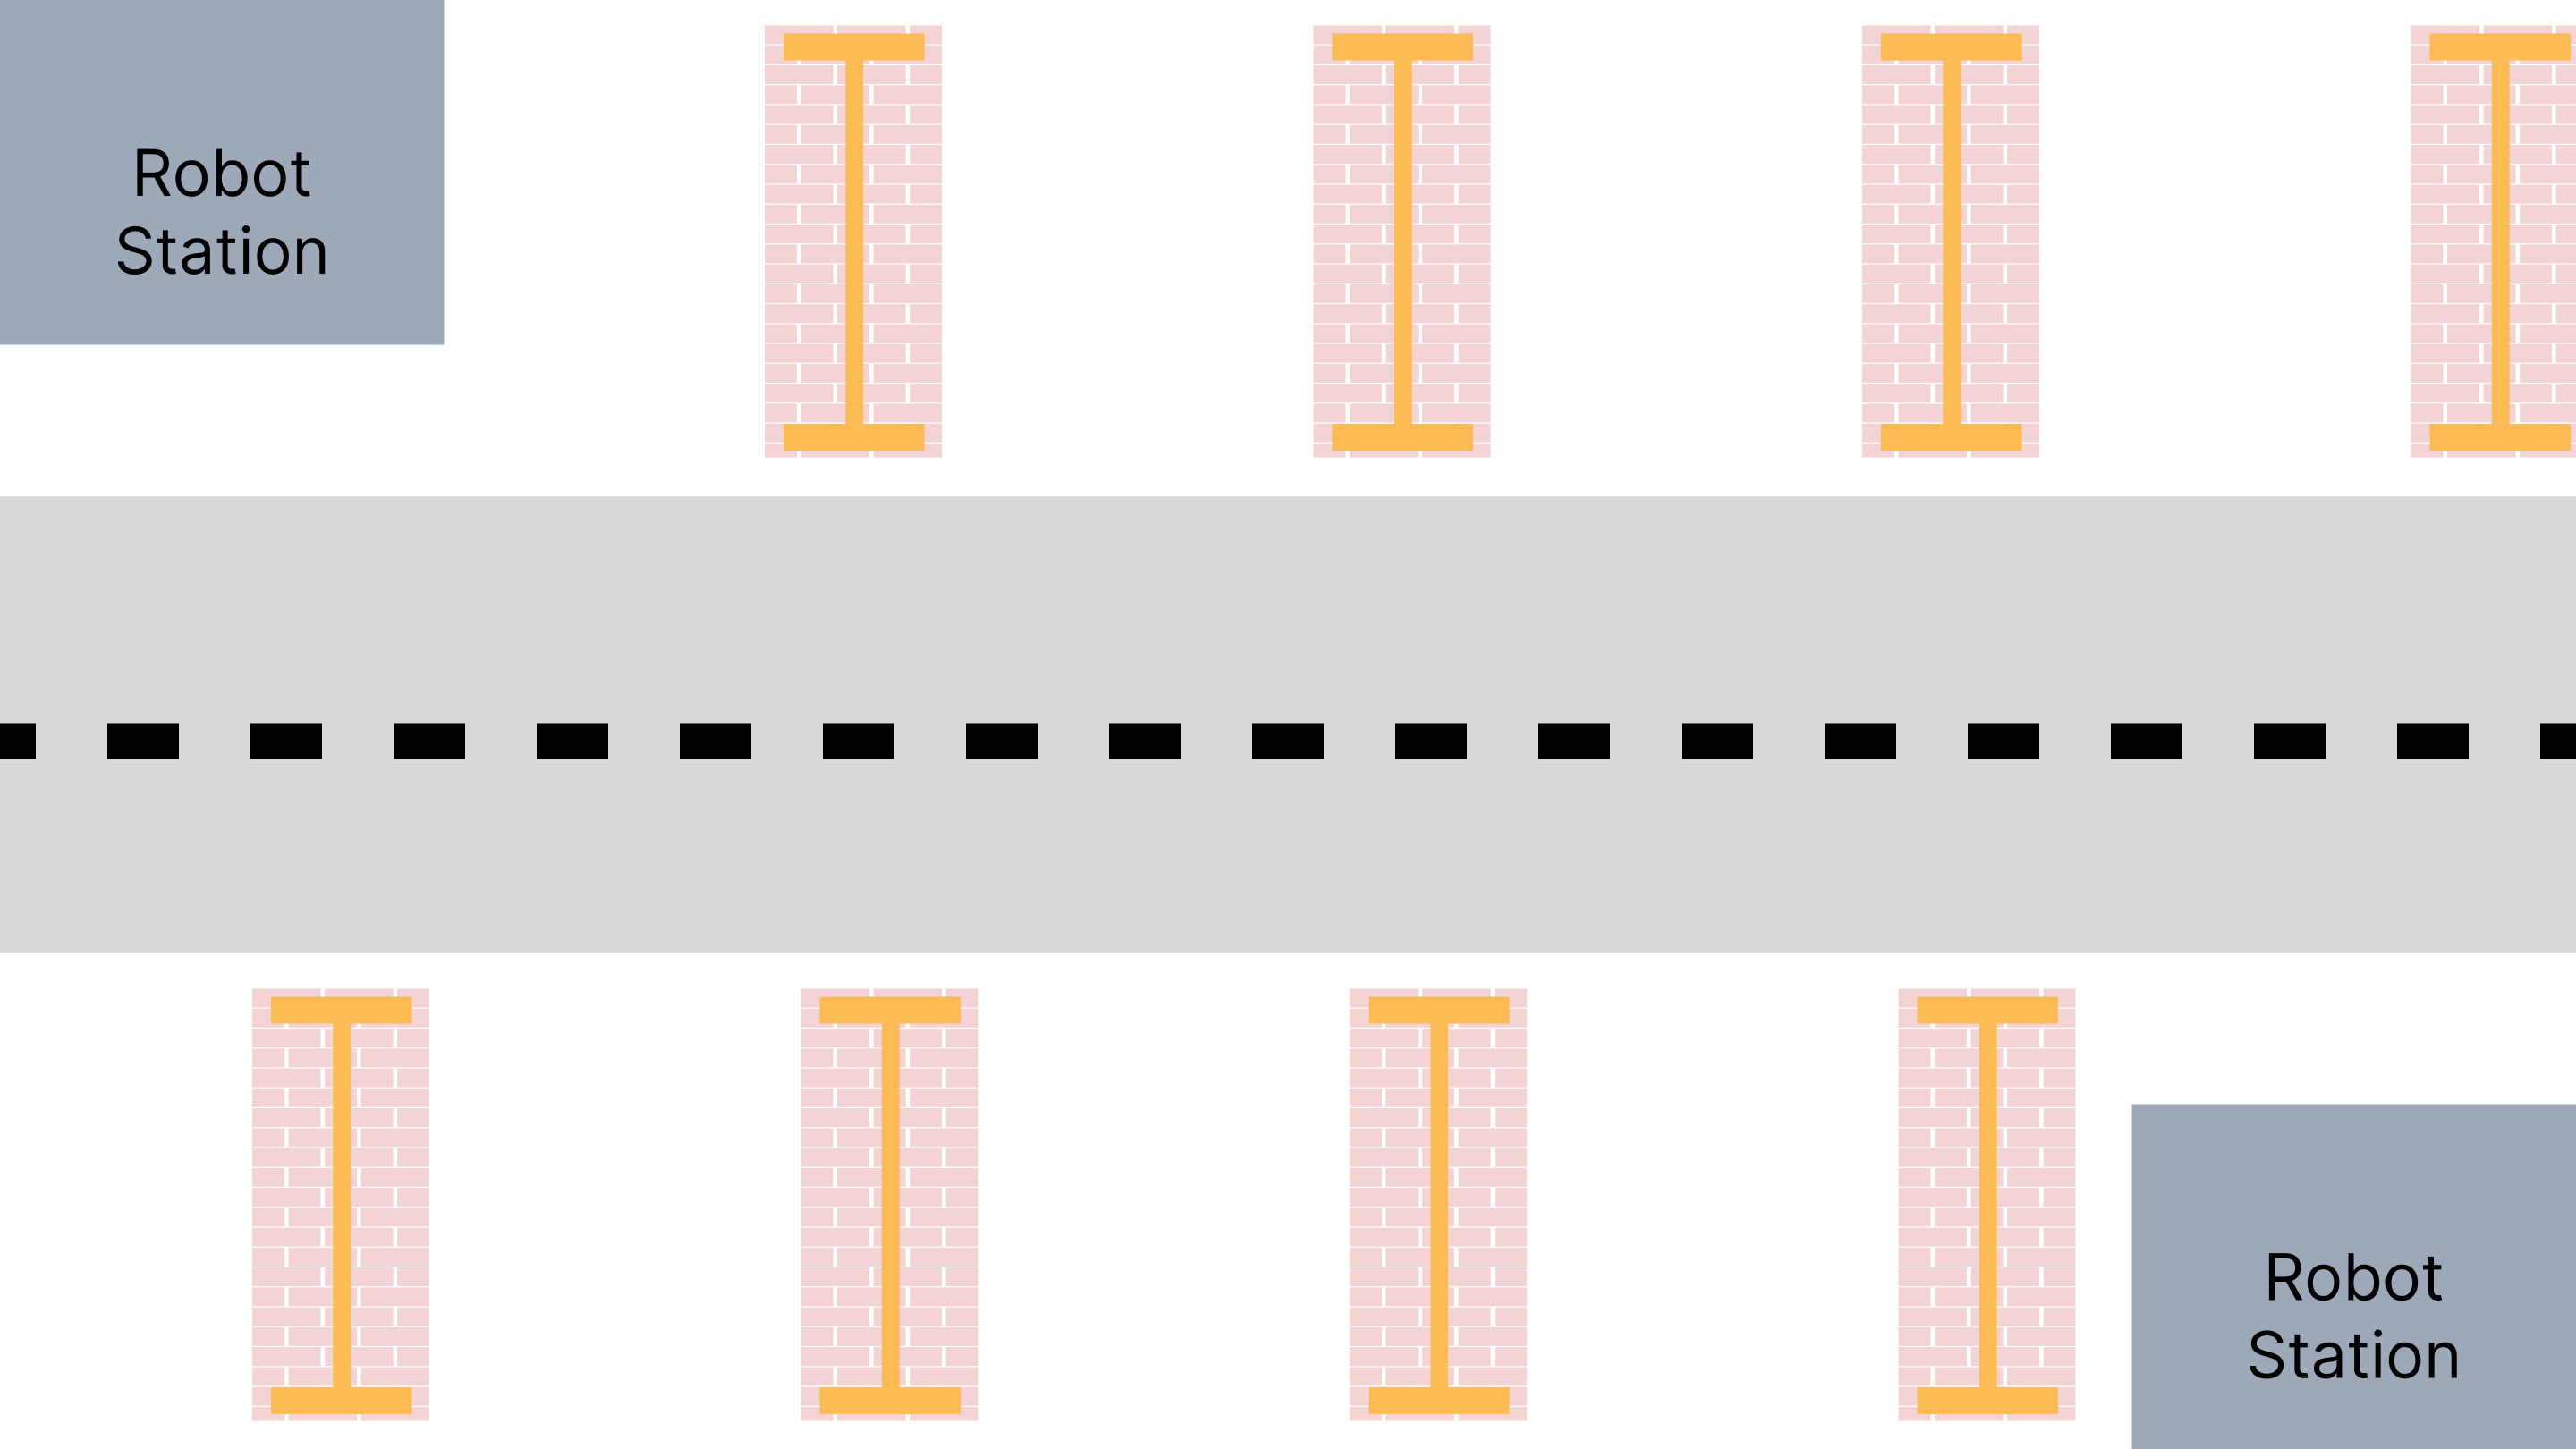
\includegraphics[width=0.88\textwidth]{Figures/report/garage_top_view.png}
\caption{Garage charging task sequence from mapping and base-station departure to local socket alignment and plug insertion.}
\label{fig:garage_top_view_placeholder}
\end{figure}

%========================mechanical_design===========================

\begin{figure}[!htbp]
\centering
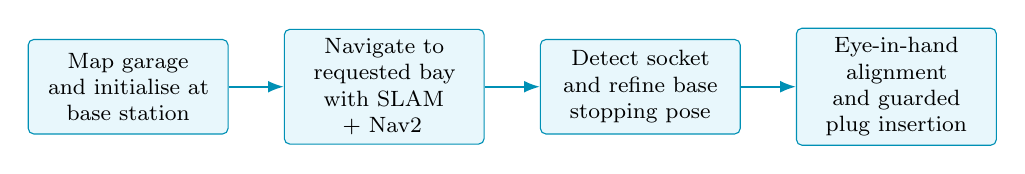
\begin{tikzpicture}[font=\footnotesize, node distance=6mm and 7mm,
  taskbox/.style={draw=accessblue, rounded corners=2pt, align=center, text width=0.19\textwidth, minimum height=12mm, fill=lightbluebox},
  taskarr/.style={-{Latex[length=2mm]}, semithick, accessblue}]
  \node[taskbox] (map) {Map garage\\and initialise at\\base station};
  \node[taskbox, right=of map] (nav) {Navigate to\\requested bay\\with SLAM + Nav2};
  \node[taskbox, right=of nav] (dock) {Detect socket\\and refine base\\stopping pose};
  \node[taskbox, right=of dock] (insert) {Eye-in-hand alignment\\and guarded\\plug insertion};
  \draw[taskarr] (map)--(nav);
  \draw[taskarr] (nav)--(dock);
  \draw[taskarr] (dock)--(insert);
\end{tikzpicture}
\caption{Operational sequence of the simplified autonomous charging task. Global navigation ends at the parking bay; the local perception and insertion stages then handle the socket-specific alignment.}
\label{fig:garage_task_sequence}
\end{figure}

% Paste this block immediately after the Task subsection.
% It is a fragment only. Do not add \documentclass, \begin{document}, or \end{document}.

\newcommand{\mechplaceholderfig}[1]{%
  \fbox{\begin{minipage}[c][0.15\textheight][c]{0.80\textwidth}\centering\itshape #1\end{minipage}}}

% Works in both text and math mode, so this fragment does not require siunitx.
\newcommand{\mechSI}[2]{\ensuremath{#1\,\mathrm{#2}}}

\subsection{Mechanical Design and Modeling}\label{sec:mechanical_design}

The mechanical design presents the physical platform and the models that describe its motion and loading. It addresses the mechanical architecture, the CAD and digital twin pipeline, the kinematic and dynamic models of the manipulator, the collision representation, and the experimental identification of the joint and motor parameters. All kinematic and dynamic relations were verified symbolically and numerically against the implementation in \texttt{works/}.

\subsubsection{Mechanical System Overview}\label{sec:mech_overview}
The robot is a mobile manipulator built from four subsystems: a differential-drive mobile base, a custom 3-DoF serial manipulator, an end-effector carrying the charging plug, and a sensor mount fixing an eye-in-hand camera to the wrist. Together they form a single kinematic chain, so every frame is expressed in one unified description. The driving design objectives are lightweight construction, ease of manufacturing, accurate simulation, and ROS~2 / Isaac Sim compatibility for autonomous charging experiments.

\begin{figure}[!htbp]
\centering
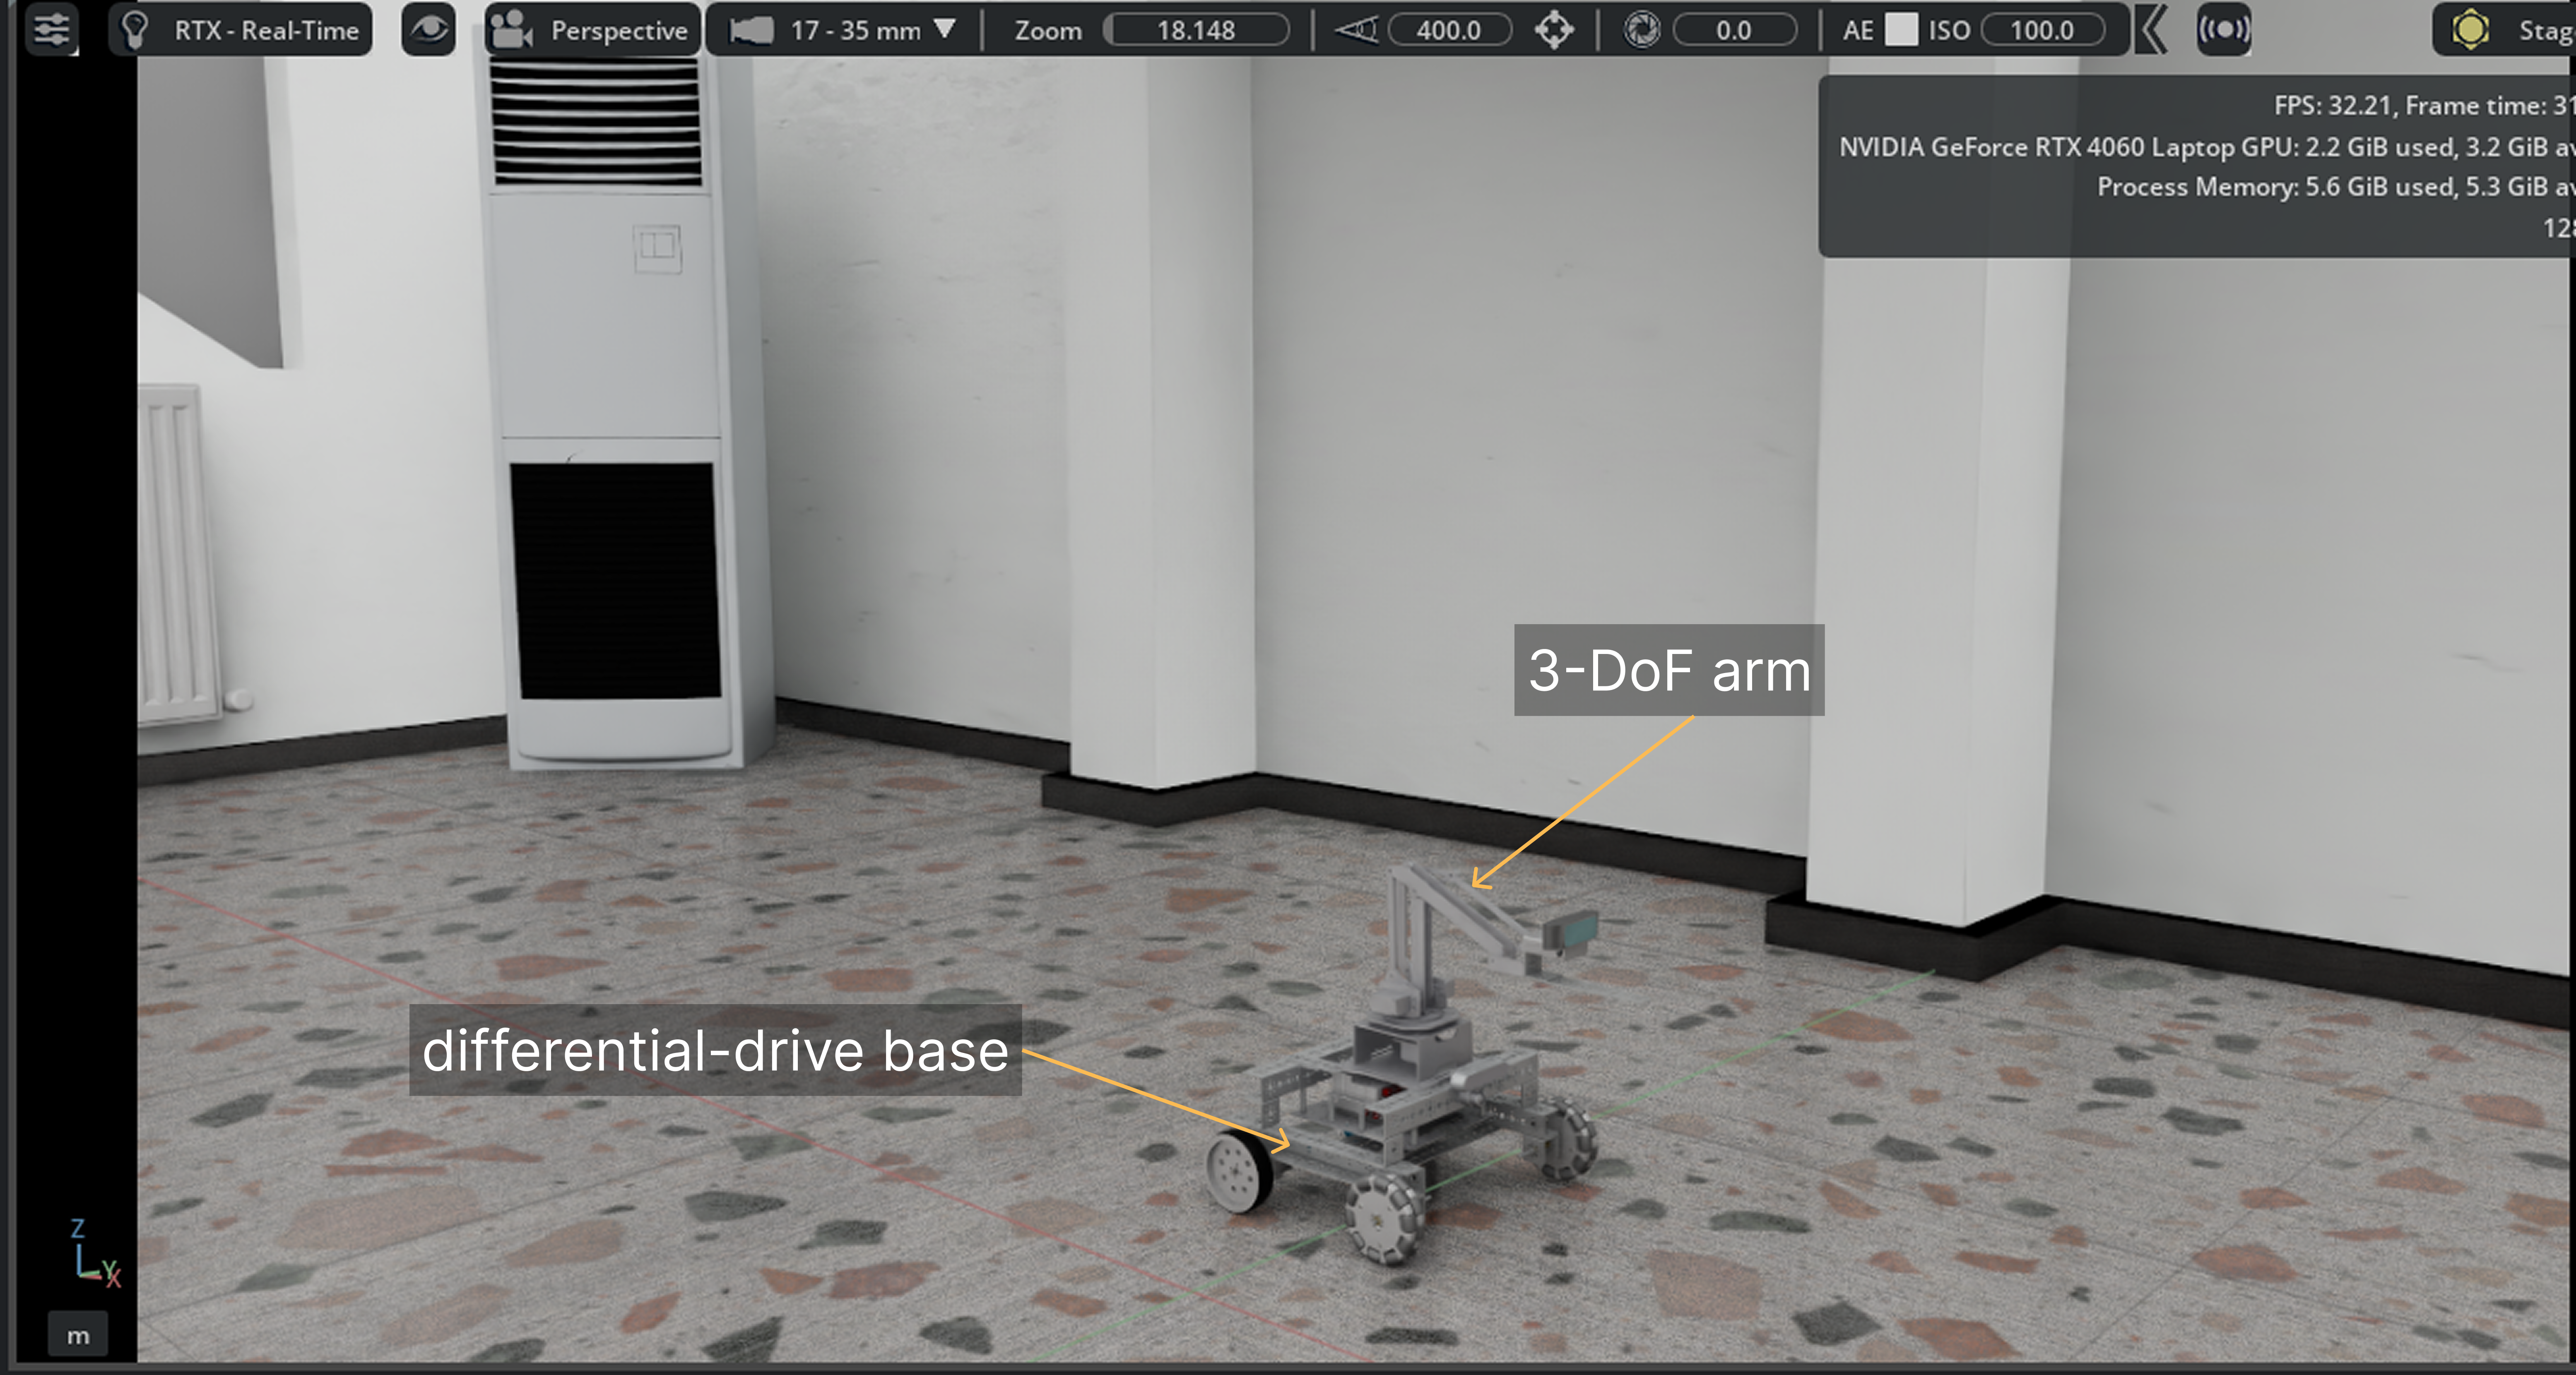
\includegraphics[width=0.72\textwidth]{Figures/report/mech_platform_overview.png}
\caption{Overview of the mobile-manipulator platform and its four subsystems.}
\label{fig:mech_platform_overview_placeholder}
\end{figure}

\subsubsection{CAD Design and Digital-Twin Development}\label{sec:cad}
Every link was modeled in Blender as a separate mesh and arranged into the parent--child hierarchy of the physical chain. The Phobos add-on exports this tree to URDF, generating the joint hierarchy, link definitions, inertial properties (\texttt{<inertial>} tags), and collision models. The same workflow is used for the base and the arm, producing one consistent description for ROS~2 and the Isaac Sim digital twin.

\begin{figure}[!htbp]
\centering
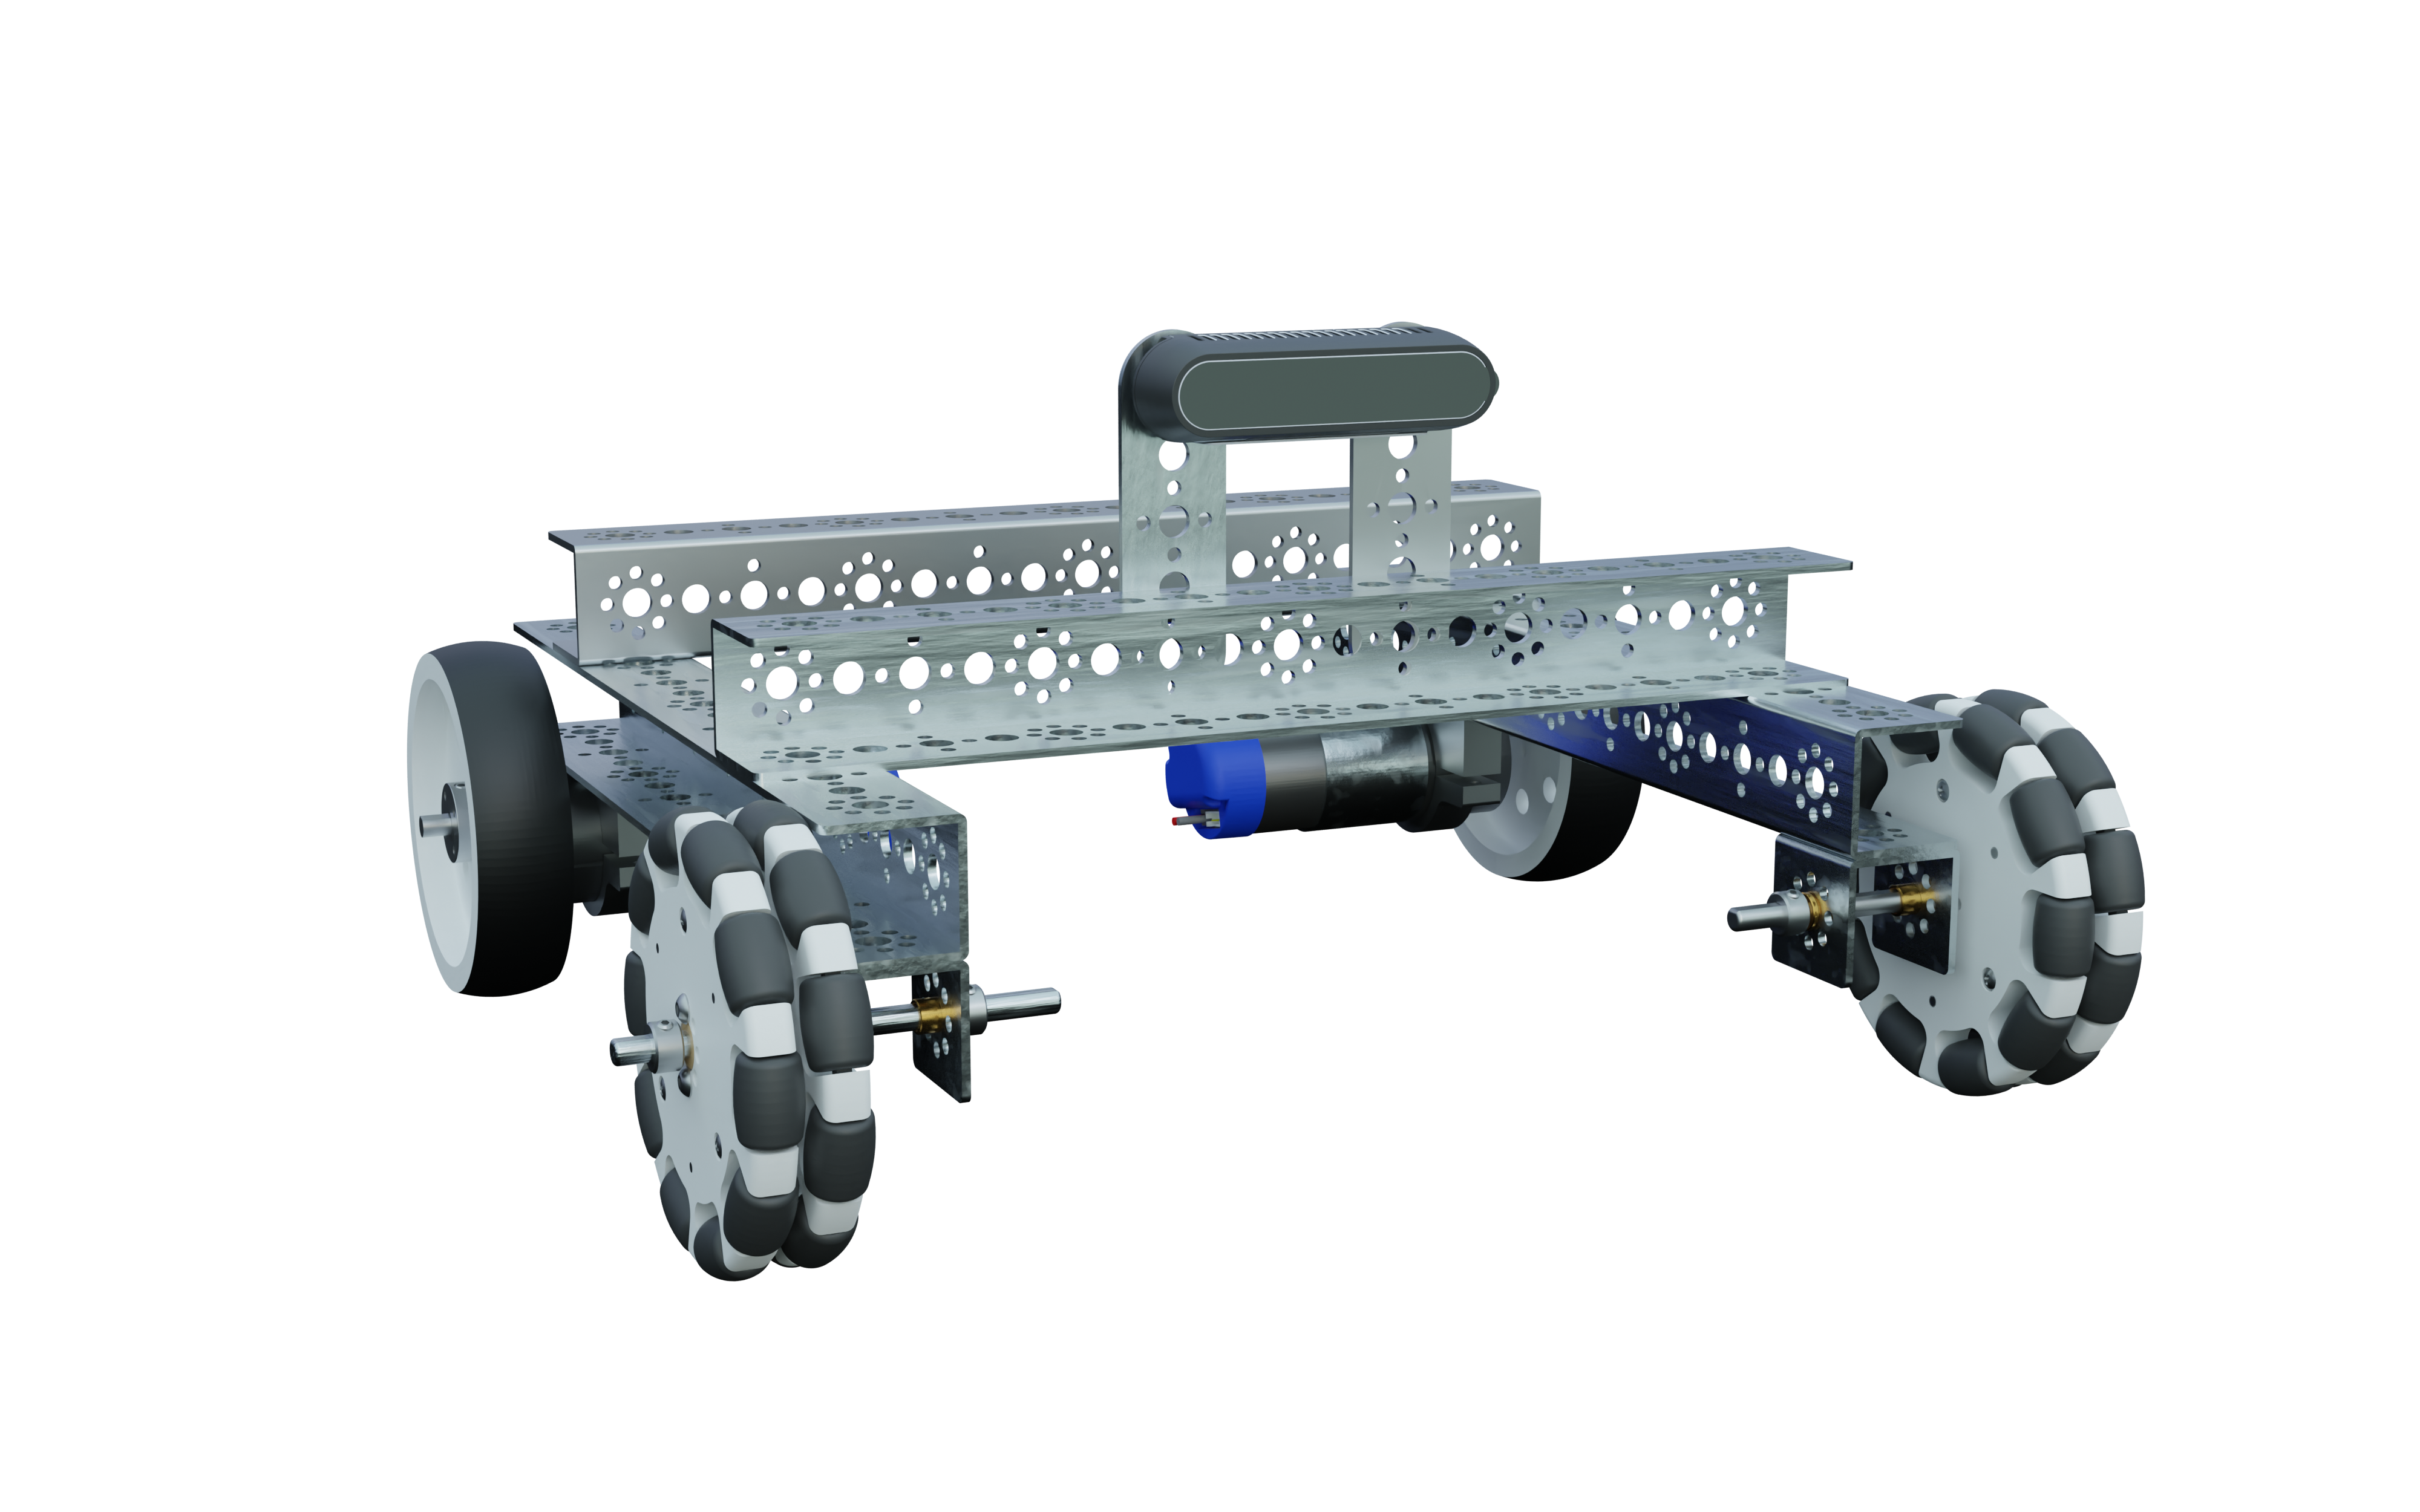
\includegraphics[width=0.82\textwidth]{Figures/blender_model.png}
\caption{Blender--Phobos--URDF pipeline producing the ROS~2 description and the Isaac Sim twin.}
\label{fig:mech_cad_urdf_placeholder}
\end{figure}

\subsubsection{Mobile Robot Mechanical Model}\label{sec:base}
The base is a differential drive. Two independently driven rear wheels set the linear and angular velocity through the sum and difference of their speeds, while passive front omni wheels provide support. The rear wheels are driven by TorqueNADO DC gear-motors, identified in Section~\ref{sec:motorid}. Mass properties are taken from CAD: the volume gives the mass,
\begin{equation}\label{eq:mass}
m=\rho\,V,
\end{equation}
and integration over the solid gives the center of mass and inertia tensor,
\begin{equation}\label{eq:inertia}
\mathbf{r}_c=\frac{1}{m}\int_{\mathcal{B}}\rho\,\mathbf{r}\,\mathrm{d}V,\qquad
\mathbf{I}=\int_{\mathcal{B}}\rho\big(\lVert\mathbf{r}-\mathbf{r}_c\rVert^2\mathbf{1}-(\mathbf{r}-\mathbf{r}_c)(\mathbf{r}-\mathbf{r}_c)^{\!\top}\big)\,\mathrm{d}V,
\end{equation}
with the inertia tensor written explicitly as
\begin{equation}\label{eq:itensor}
\mathbf{I}=\begin{bmatrix} I_{xx}&-I_{xy}&-I_{xz}\\ -I_{xy}&I_{yy}&-I_{yz}\\ -I_{xz}&-I_{yz}&I_{zz}\end{bmatrix}.
\end{equation}
These are written automatically into each link's \texttt{<inertial>} tag. Accurate inertia is essential because simulated acceleration scales inversely with it, so motion prediction and controller tuning both depend on it.

\begin{figure}[!htbp]
\centering
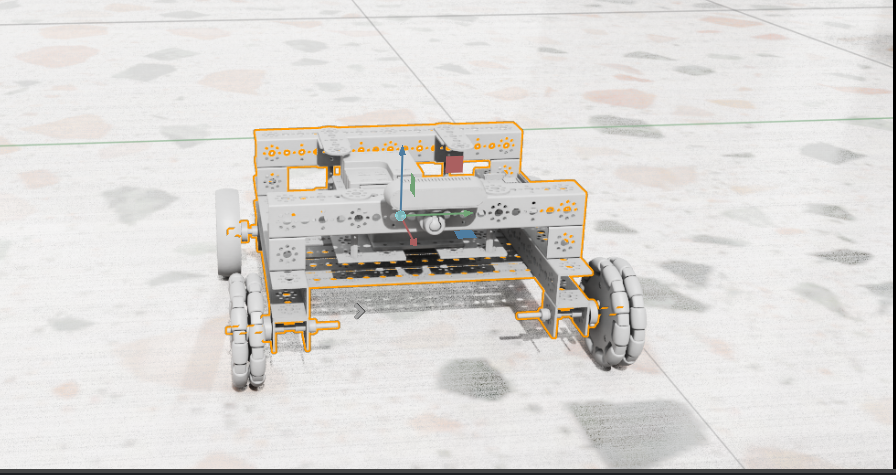
\includegraphics[width=0.88\textwidth]{Figures/report/mech_base_mass.png}
\caption{Mobile-base mass properties extracted from CAD and the differential-drive layout.}
\label{fig:mech_base_mass_placeholder}
\end{figure}

Table~\ref{tab:base_specs} lists the geometric and inertial properties of the mobile base as measured from the composed USD model in Isaac~Sim~5.1 using PhysX auto-computed world bounds. The base is a 2-wheel differential-drive platform: the two rear \texttt{\_9055} wheels are actively driven while the two front \texttt{\_6466} dual-omni wheels act as passive casters. The geometric drive track of 357\,mm represents the physical wheel-centre spacing; the controller's \emph{effective} turn track was calibrated to approximately 560\,mm to compensate for skid during in-place pivots.

\begin{table}[!htbp]
\centering
\caption{Mobile-robot base specifications measured in Isaac~Sim~5.1 (PhysX, USD world bounds).}
\label{tab:base_specs}
\small
\setlength{\tabcolsep}{5pt}
\begin{tabular}{@{}ll@{}}
\toprule
Property & Value \\
\midrule
Base link mass & 4.5\,kg \\
Total robot mass (base + 4 wheels) & 5.164\,kg \\
Dimensions (L\,$\times$\,W\,$\times$\,H) & $300 \times 382 \times 173$\,mm \\
Height span above floor & 25\,mm -- 198\,mm \\
Center of mass (base-link frame) & $(-1.2,\ 0.5,\ 30.9)$\,mm \\
Rear (drive) track, centre-to-centre & 357\,mm \\
Front track & 352\,mm \\
Wheelbase (rear $\to$ front axle) & 237\,mm \\
Effective turn track (calibrated) & $\approx 560$\,mm \\
\bottomrule
\end{tabular}
\end{table}

\begin{table}[!htbp]
\centering
\caption{Wheel specifications of the mobile base.}
\label{tab:wheel_specs}
\small
\setlength{\tabcolsep}{4pt}
\begin{tabular}{@{}llccc@{}}
\toprule
Wheel & Count & Role & Mass (each) & Diameter\,$\times$\,Width \\
\midrule
Rear (\texttt{\_9055})  & 2 & Differential drive       & 0.132\,kg & $101.6 \times 26.4$\,mm \\
Front (\texttt{\_6466}) & 2 & Dual-omni passive caster & 0.200\,kg & $104.8 \times 30.7$\,mm \\
\bottomrule
\end{tabular}
\end{table}

\subsubsection{Collision Modeling}\label{sec:collision}
Visual meshes (high-detail, for rendering) are separated from collision meshes (simplified, for contact). Contact is represented by a signed distance field, negative inside the body and positive outside,
\begin{equation}\label{eq:sdf}
\Phi(\mathbf{x})=\begin{cases}+\,\mathrm{dist}(\mathbf{x},\partial\mathcal{B}) & \mathbf{x}\notin\mathcal{B},\\ -\,\mathrm{dist}(\mathbf{x},\partial\mathcal{B}) & \mathbf{x}\in\mathcal{B},\end{cases}
\end{equation}
whose zero level set is the surface and whose gradient $\nabla\Phi$ is the contact normal. Compared with primitive proxies, the SDF gives continuous collision detection, accurate ground contact, better stability, and less interpenetration. This matters for the wheel--ground, arm--environment, and plug--socket contacts, whose clearances are only millimeters.

\begin{figure}[!htbp]
\centering
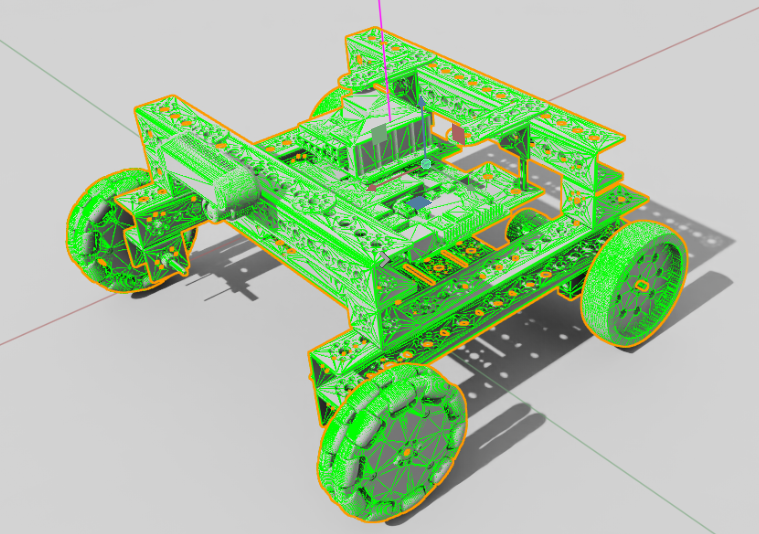
\includegraphics[width=0.88\textwidth]{Figures/report/mech_sdf.png}
\caption{Visual mesh versus the SDF collision representation used in Isaac Sim.}
\label{fig:mech_sdf_placeholder}
\end{figure}

\subsubsection{Manipulator Mechanical Design}\label{sec:manip}
The arm is a 3-DoF serial chain with link lengths
\begin{equation}\label{eq:dims}
L_0=\mechSI{84.4}{mm},\ L_1=\mechSI{8.14}{mm},\ L_2=\mechSI{128.4}{mm},\ L_3=\mechSI{138.0}{mm},\ L_4=\mechSI{16.8}{mm}.
\end{equation}
Because $L_1$ and $L_4$ are horizontal offsets in the plane of motion they enter only as their sum,
\begin{equation}\label{eq:r0}
r_0=L_1+L_4=\mechSI{24.94}{mm}.
\end{equation}
Joint~1 is base yaw, Joint~2 shoulder pitch, Joint~3 elbow pitch. A fourth, passive wrist is mechanically coupled to the two pitch joints,
\begin{equation}\label{eq:passive}
\theta_{3,\text{passive}}=270^{\circ}-\theta_1-\theta_2-90^{\circ}=180^{\circ}-\theta_1-\theta_2,
\end{equation}
where the fixed $270^{\circ}$ and $90^{\circ}$ terms are the constant offsets set by the linkage geometry. This coupling keeps the plug level (fixed orientation) as the arm reconfigures, so the mechanism has three controllable DoF despite four moving joints.
The passive wrist is realized as a planar four-link mechanism that mechanically couples the wrist
to the shoulder and elbow motions. As the two active pitch joints rotate, the linkage drives the
final link so that the plug mounting plate remains approximately level throughout the motion.
This removes the need for a fourth actuator while preserving the orientation constraint required
for plug--socket alignment in the laboratory charging task.

\begin{figure}[t]
\centering
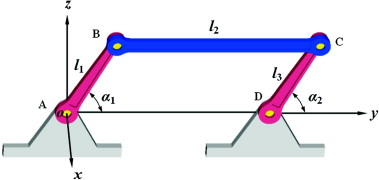
\includegraphics[width=0.82\textwidth]{Figures/report/passive_wrist_fourlink.png}
\caption{Passive wrist implemented as a four-link mechanism that preserves the plug orientation
while the shoulder and elbow joints move.}
\label{fig:passive_wrist_fourlink}
\end{figure}
\begin{figure}[!htbp]
\centering
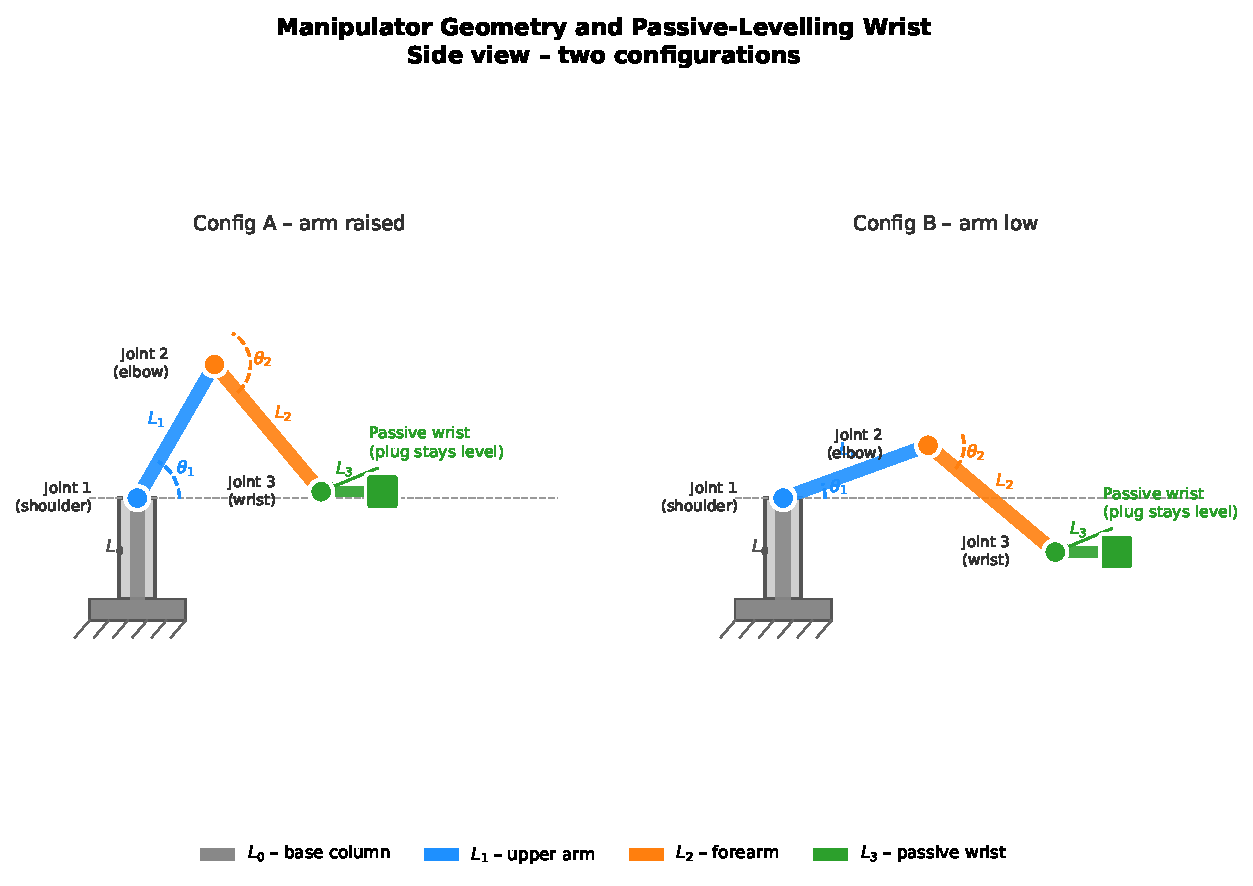
\includegraphics[width=0.88\textwidth]{Figures/report/fig_arm_geometry.png}
\caption{Manipulator geometry, link lengths, and the passive leveling wrist.}
\label{fig:mech_arm_geometry_placeholder}
\end{figure}



\subsubsection{Forward Kinematics}\label{sec:fk}
Composing homogeneous transforms along the chain (with $c_i=\cos\theta_i,\ s_i=\sin\theta_i$),
\begin{equation}\label{eq:T01}
T_{01}=R_z(\theta_1)\,\mathrm{Trans}(r_0,0,L_0)=
\begin{bmatrix} c_1&-s_1&0&r_0c_1\\ s_1&c_1&0&r_0s_1\\ 0&0&1&L_0\\ 0&0&0&1\end{bmatrix},
\end{equation}
\begin{equation}\label{eq:T12}
\begin{aligned}
T_{12}&=R_y(\theta_2)\,\mathrm{Trans}(0,0,L_2)=
\begin{bmatrix} c_2&0&s_2&L_2s_2\\ 0&1&0&0\\ -s_2&0&c_2&L_2c_2\\ 0&0&0&1\end{bmatrix},\\[4pt]
T_{23}&=R_y(\theta_3)\,\mathrm{Trans}(0,0,L_3)=
\begin{bmatrix} c_3&0&s_3&L_3s_3\\ 0&1&0&0\\ -s_3&0&c_3&L_3c_3\\ 0&0&0&1\end{bmatrix}.
\end{aligned}
\end{equation}
The passive-wrist transform $T_{34}=R_y(\theta_{3,\text{passive}})$ acts at the wrist origin and does not move it. Multiplying the three transforms $T_{01}T_{12}T_{23}$ and reading off the translation column gives the closed-form wrist position
\begin{equation}\label{eq:fk}
\boxed{\;
\begin{aligned}
\rho(\theta_2,\theta_3)&=r_0+L_2\sin\theta_2+L_3\sin(\theta_2+\theta_3),\\
x&=\rho\cos\theta_1,\qquad y=\rho\sin\theta_1,\\
z(\theta_2,\theta_3)&=L_0+L_2\cos\theta_2+L_3\cos(\theta_2+\theta_3).
\end{aligned}\;}
\end{equation}
Here $\rho$ is the radial reach (shoulder and elbow projections plus the offset $r_0$), $z$ the height, and the base yaw $\theta_1$ only rotates that reach into $x,y$. This closed form equals the full transform product exactly.

\begin{figure}[!htbp]
\centering
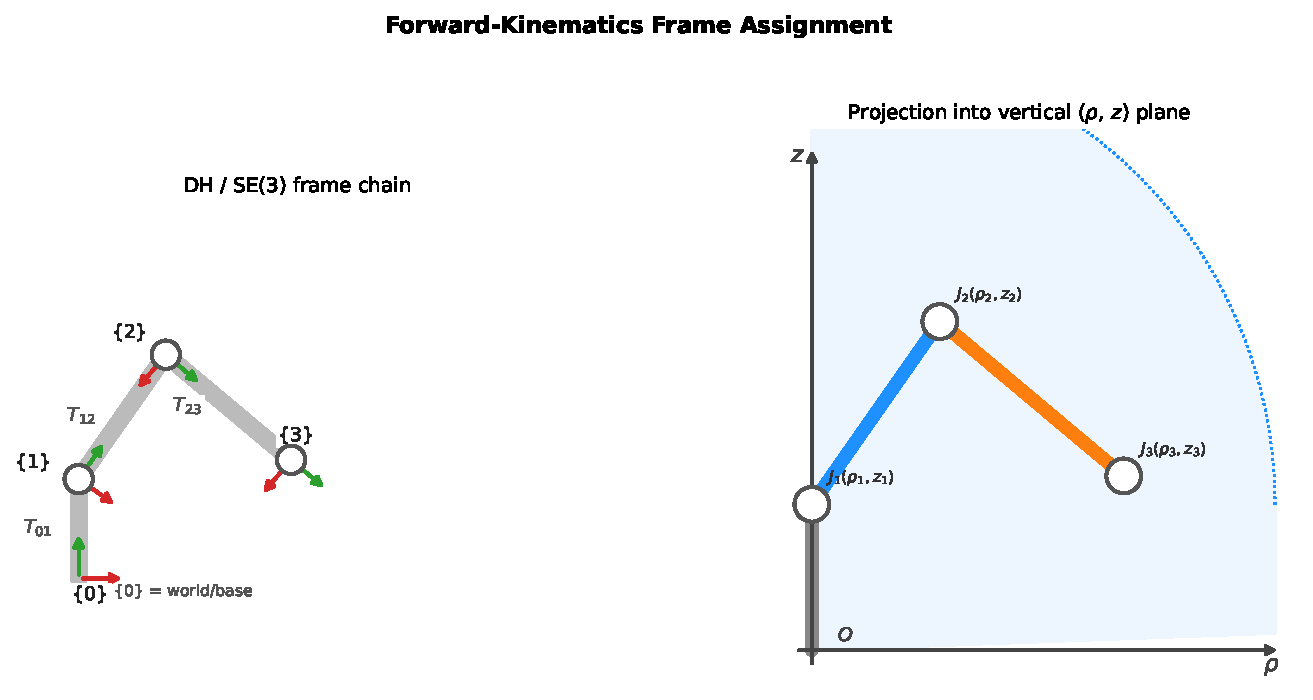
\includegraphics[width=0.88\textwidth]{Figures/report/fig_fk_frames.png}
\caption{Frame assignment and the planar $(\rho,z)$ projection used in the forward kinematics.}
\label{fig:mech_fk_frames_placeholder}
\end{figure}

\subsubsection{Inverse Kinematics}\label{sec:ik}
The base yaw is set by the target azimuth,
\begin{equation}\label{eq:ik1}
\theta_1=\operatorname{atan2}(y_d,x_d),
\end{equation}
and the planar wrist coordinates relative to the shoulder are
\begin{equation}\label{eq:ikuw}
u=\sqrt{x_d^2+y_d^2}-r_0,\qquad w=z_d-L_0.
\end{equation}
The law of cosines on the triangle $(L_2,L_3,D)$ with $D=\sqrt{u^2+w^2}$ gives the elbow,
\begin{equation}\label{eq:ikelbow}
\theta_3=\mp\arccos\!\left(\frac{u^2+w^2-L_2^2-L_3^2}{2L_2L_3}\right),
\end{equation}
the two signs being elbow-up and elbow-down, and the shoulder follows as
\begin{equation}\label{eq:ik2}
\theta_2=\operatorname{atan2}(u,w)-\operatorname{atan2}\!\big(L_3\sin\theta_3,\,L_2+L_3\cos\theta_3\big).
\end{equation}
Round-tripping through the forward map over $5\times10^4$ targets gave a worst error of $1.4\times10^{-16}\,\mathrm{m}$. Singularities occur at full extension/folding ($D=L_2+L_3$ or $|L_2-L_3|$) and on the base axis; the reachable shell is $|L_2-L_3|\le D\le L_2+L_3$, i.e.\ $\mechSI{9.6}{mm}\le D\le\mechSI{266.4}{mm}$.

\begin{figure}[!htbp]
\centering
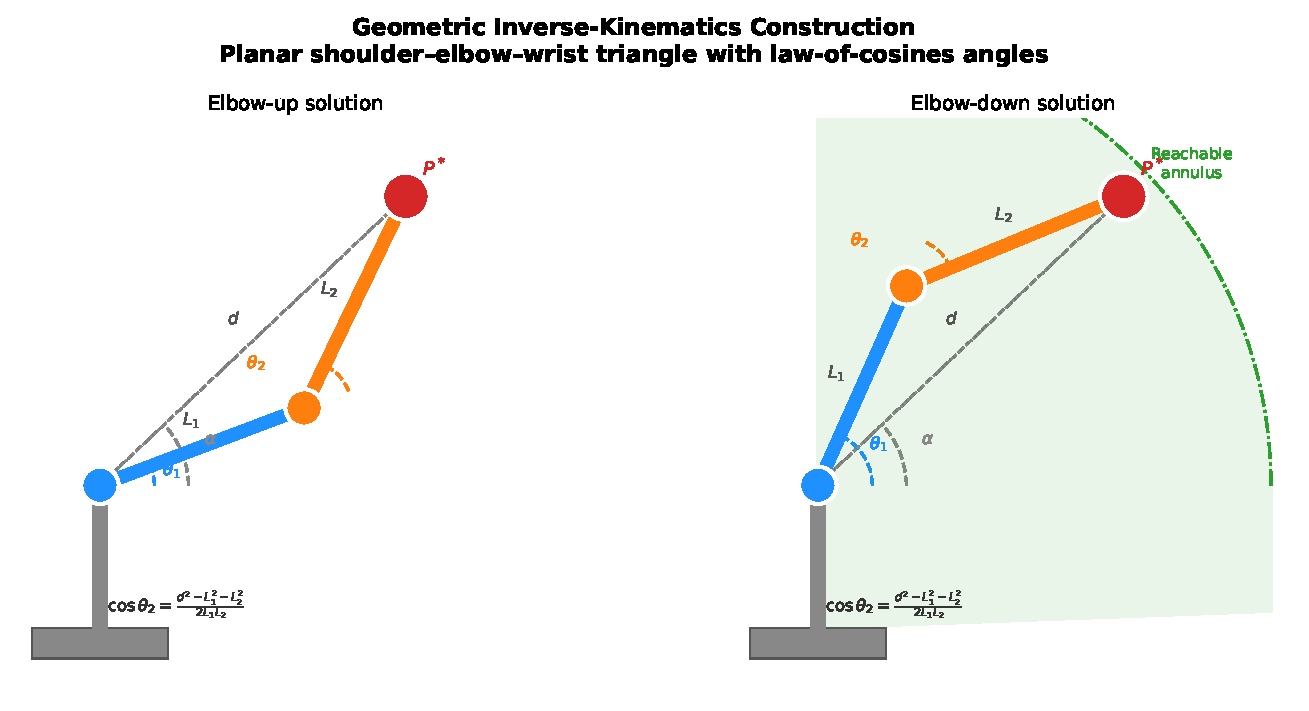
\includegraphics[width=0.88\textwidth]{Figures/report/fig_ik_geometry.png}
\caption{Geometric inverse kinematics: law-of-cosines construction and the two elbow branches.}
\label{fig:mech_ik_geometry_placeholder}
\end{figure}

\subsubsection{Jacobian Analysis}\label{sec:jac}
Differentiating the forward map, $\dot{\mathbf{p}}=J(\mathbf{q})\dot{\mathbf{q}}$ with ($c_{23}=\cos(\theta_2+\theta_3),\ s_{23}=\sin(\theta_2+\theta_3)$)
\begin{equation}\label{eq:jac}
J(\mathbf{q})=\begin{bmatrix}
-\rho s_1 & c_1(L_2c_2+L_3c_{23}) & c_1L_3c_{23}\\
\rho c_1 & s_1(L_2c_2+L_3c_{23}) & s_1L_3c_{23}\\
0 & -(L_2s_2+L_3s_{23}) & -L_3s_{23}\end{bmatrix}.
\end{equation}
Its determinant evaluates to
\begin{equation}\label{eq:detj}
\det J(\mathbf{q})=\rho\,L_2L_3\sin\theta_3,
\end{equation}
so the arm is singular when $\sin\theta_3=0$ (elbow straight/folded) or $\rho=0$ (wrist on the base axis). Because $J$ is square, the manipulability measure reduces to the absolute determinant,
\begin{equation}\label{eq:manip}
\mu=\sqrt{\det(JJ^\top)}=|\det J|=\rho\,L_2L_3|\sin\theta_3|,
\end{equation}
maximal near $\theta_3=\pm90^{\circ}$ and zero at singularities, where positioning sensitivity is worst.

\begin{figure}[!htbp]
\centering
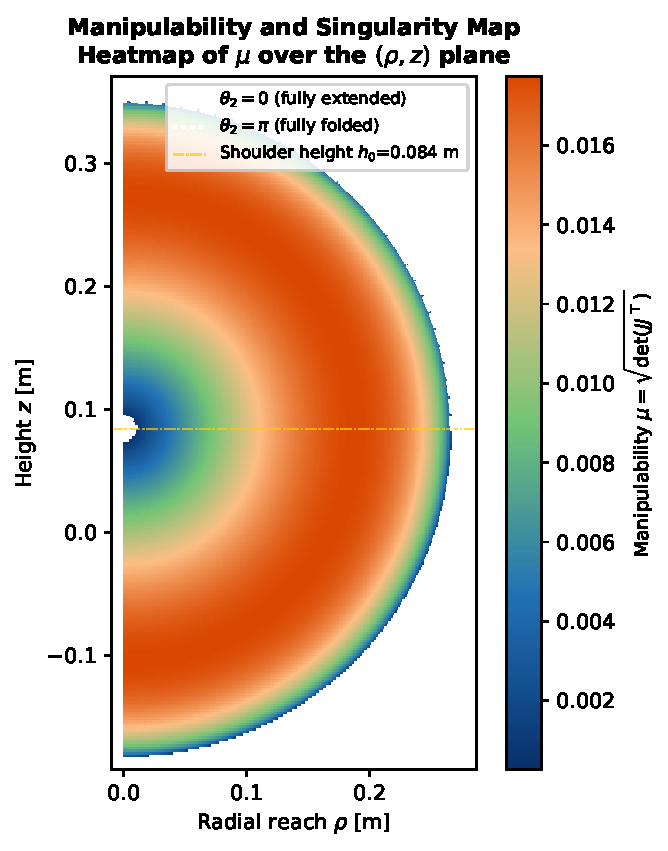
\includegraphics[width=0.82\textwidth]{Figures/report/fig_manipulability.png}
\caption{Manipulability distribution and singular configurations of the manipulator.}
\label{fig:mech_manipulability_placeholder}
\end{figure}

\subsubsection{Dynamic Modeling}\label{sec:dyn}
For the gravity-loaded planar two-link subsystem (shoulder $\theta_1$, elbow $\theta_2$; $l_1=L_2,\ l_2=L_3$), the Euler--Lagrange equations give
\begin{equation}\label{eq:eom}
M(\mathbf{q})\ddot{\mathbf{q}}+C(\mathbf{q},\dot{\mathbf{q}})\dot{\mathbf{q}}+G(\mathbf{q})=\boldsymbol{\tau},
\end{equation}
with the inertia matrix
\begin{equation}\label{eq:M}
M(\mathbf{q})=\begin{bmatrix}
I_1+I_2+m_1l_{c1}^2+m_2(l_1^2+l_{c2}^2+2l_1l_{c2}\cos\theta_2) & I_2+m_2(l_{c2}^2+l_1l_{c2}\cos\theta_2)\\
I_2+m_2(l_{c2}^2+l_1l_{c2}\cos\theta_2) & I_2+m_2l_{c2}^2\end{bmatrix},
\end{equation}
the Coriolis/centrifugal matrix
\begin{equation}\label{eq:C}
C(\mathbf{q},\dot{\mathbf{q}})=\begin{bmatrix} h\dot\theta_2 & h(\dot\theta_1+\dot\theta_2)\\ -h\dot\theta_1 & 0\end{bmatrix},\qquad h=-m_2l_1l_{c2}\sin\theta_2,
\end{equation}
and the gravity vector
\begin{equation}\label{eq:G}
G(\mathbf{q})=\begin{bmatrix} (m_1l_{c1}+m_2l_1)g\cos\theta_1+m_2l_{c2}g\cos(\theta_1+\theta_2)\\ m_2l_{c2}g\cos(\theta_1+\theta_2)\end{bmatrix}.
\end{equation}
The diagonal of $M$ is the effective inertia at each joint, and the off-diagonal entries are the inter-joint coupling; both scale with $\cos\theta_2$. The matrix $C$ holds the velocity-dependent torques. The vector $G$ is the gravity hold-torque, which is largest with a link horizontal and reaches $\approx\mechSI{0.4}{N.m}$ at the shoulder when fully extended. The passive wrist adds no equation: its mass, inertia, and gravity term are reflected into the shoulder and elbow through the coupling, so two dynamic equations describe all four moving bodies.

\begin{figure}[!htbp]
\centering
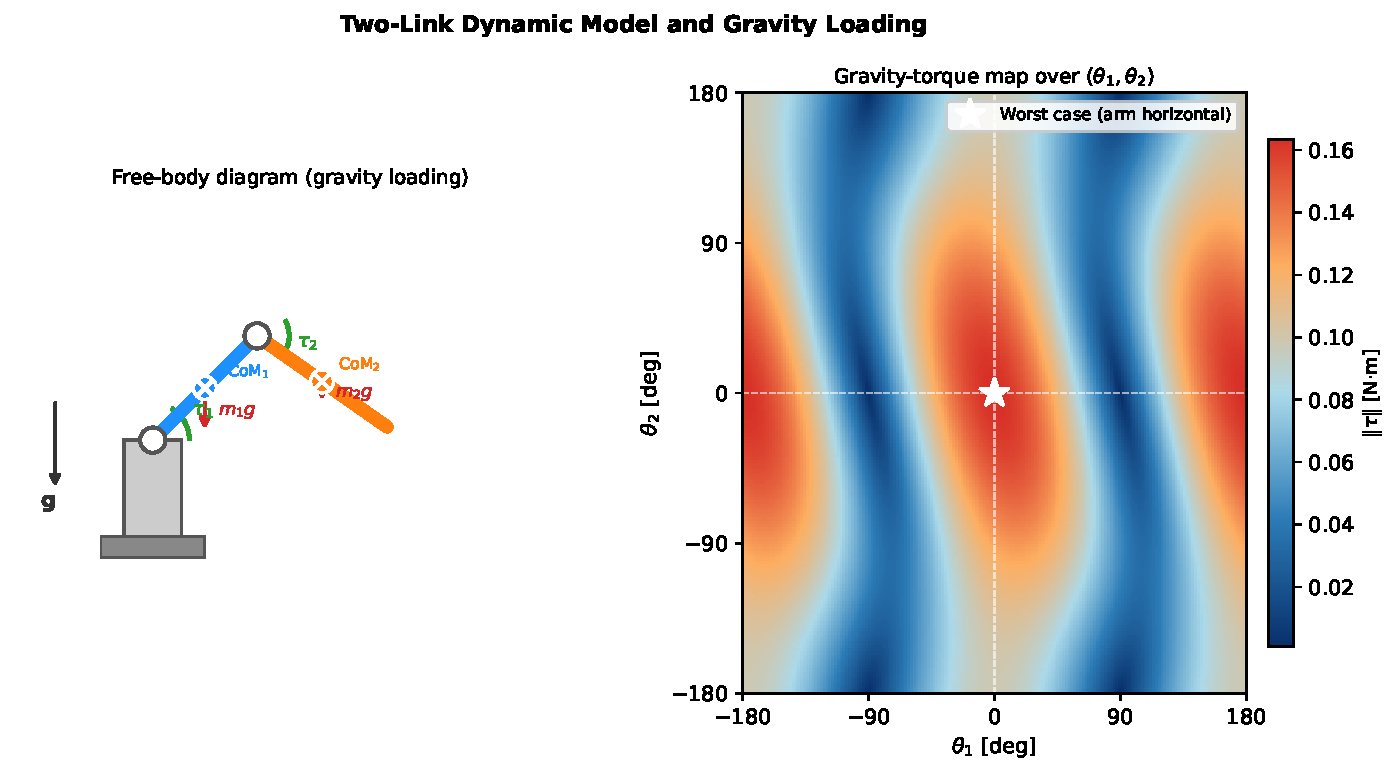
\includegraphics[width=0.88\textwidth]{Figures/report/fig_dynamics.png}
\caption{Two-link dynamic model and the configuration-dependent gravity load.}
\label{fig:mech_dynamics_placeholder}
\end{figure}

\subsubsection{Joint Characterization Experiments}\label{sec:jointid}
Each servo joint is a second-order system,
\begin{equation}\label{eq:jointmodel}
J\ddot\theta+b\dot\theta+k\theta=\tau.
\end{equation}
Four experiments identify the inertia $J$, damping $b$, and stiffness $k$: a step response, a free oscillation, a frequency sweep, and a static deflection test.

\textbf{Experiment 1: Step response.} The ESP32 commands a position step and streams $(t,\theta)$; the data is Savitzky--Golay smoothed and fitted to the full second-order step response
\begin{equation}\label{eq:stepform}
\theta(t)=\theta_0+(\theta_f-\theta_0)\,g(t),
\end{equation}
with $g(t)$ underdamped, critically damped, or overdamped,
\begin{equation}\label{eq:gforms}
g_{\zeta<1}=1-e^{-\zeta\omega_n t}\!\Big[\cos\omega_d t+\tfrac{\zeta}{\sqrt{1-\zeta^2}}\sin\omega_d t\Big],\quad
g_{\zeta=1}=1-e^{-\omega_n t}(1+\omega_n t),\quad
g_{\zeta>1}=1+\tfrac{s_1e^{s_2t}-s_2e^{s_1t}}{s_2-s_1},
\end{equation}
where $\omega_d=\omega_n\sqrt{1-\zeta^2}$ and $s_{1,2}=-\omega_n(\zeta\mp\sqrt{\zeta^2-1})$. The parameters $(\theta_0,\theta_f,\zeta,\omega_n)$ minimize
\begin{equation}\label{eq:lscost}
\mathcal{J}=\frac{1}{N}\sum_{k=1}^{N}\big[\theta_{\text{meas}}(t_k)-\theta(t_k)\big]^2
\end{equation}
by multi-start Nelder--Mead. With the inertia $J$ known, the stiffness and damping follow:
\begin{equation}\label{eq:kb}
k=J\,\omega_n^2,\qquad b=2\zeta J\omega_n.
\end{equation}

\textbf{Experiment 2: Free oscillation.} An unpowered release decays as $\theta=\theta_0e^{-\zeta\omega_n t}\cos(\omega_d t+\varphi)$; the logarithmic decrement gives the damping,
\begin{equation}\label{eq:logdec}
\delta=\ln\frac{x_n}{x_{n+1}},\qquad \zeta=\frac{\delta}{\sqrt{4\pi^2+\delta^2}}.
\end{equation}

\textbf{Experiment 3: Frequency response.} A swept sinusoid yields the Bode plot, giving the resonance frequency, bandwidth, and dynamic stiffness.

\textbf{Experiment 4: Static deflection.} Known torques at zero speed give the stiffness directly,
\begin{equation}\label{eq:static}
k=\frac{\tau}{\Delta\theta},
\end{equation}
and $1/k$ is the compliance that lets the rigid arm absorb small insertion misalignments.

\begin{figure}[!htbp]
\centering
\begin{subfigure}[b]{0.60\textwidth}
  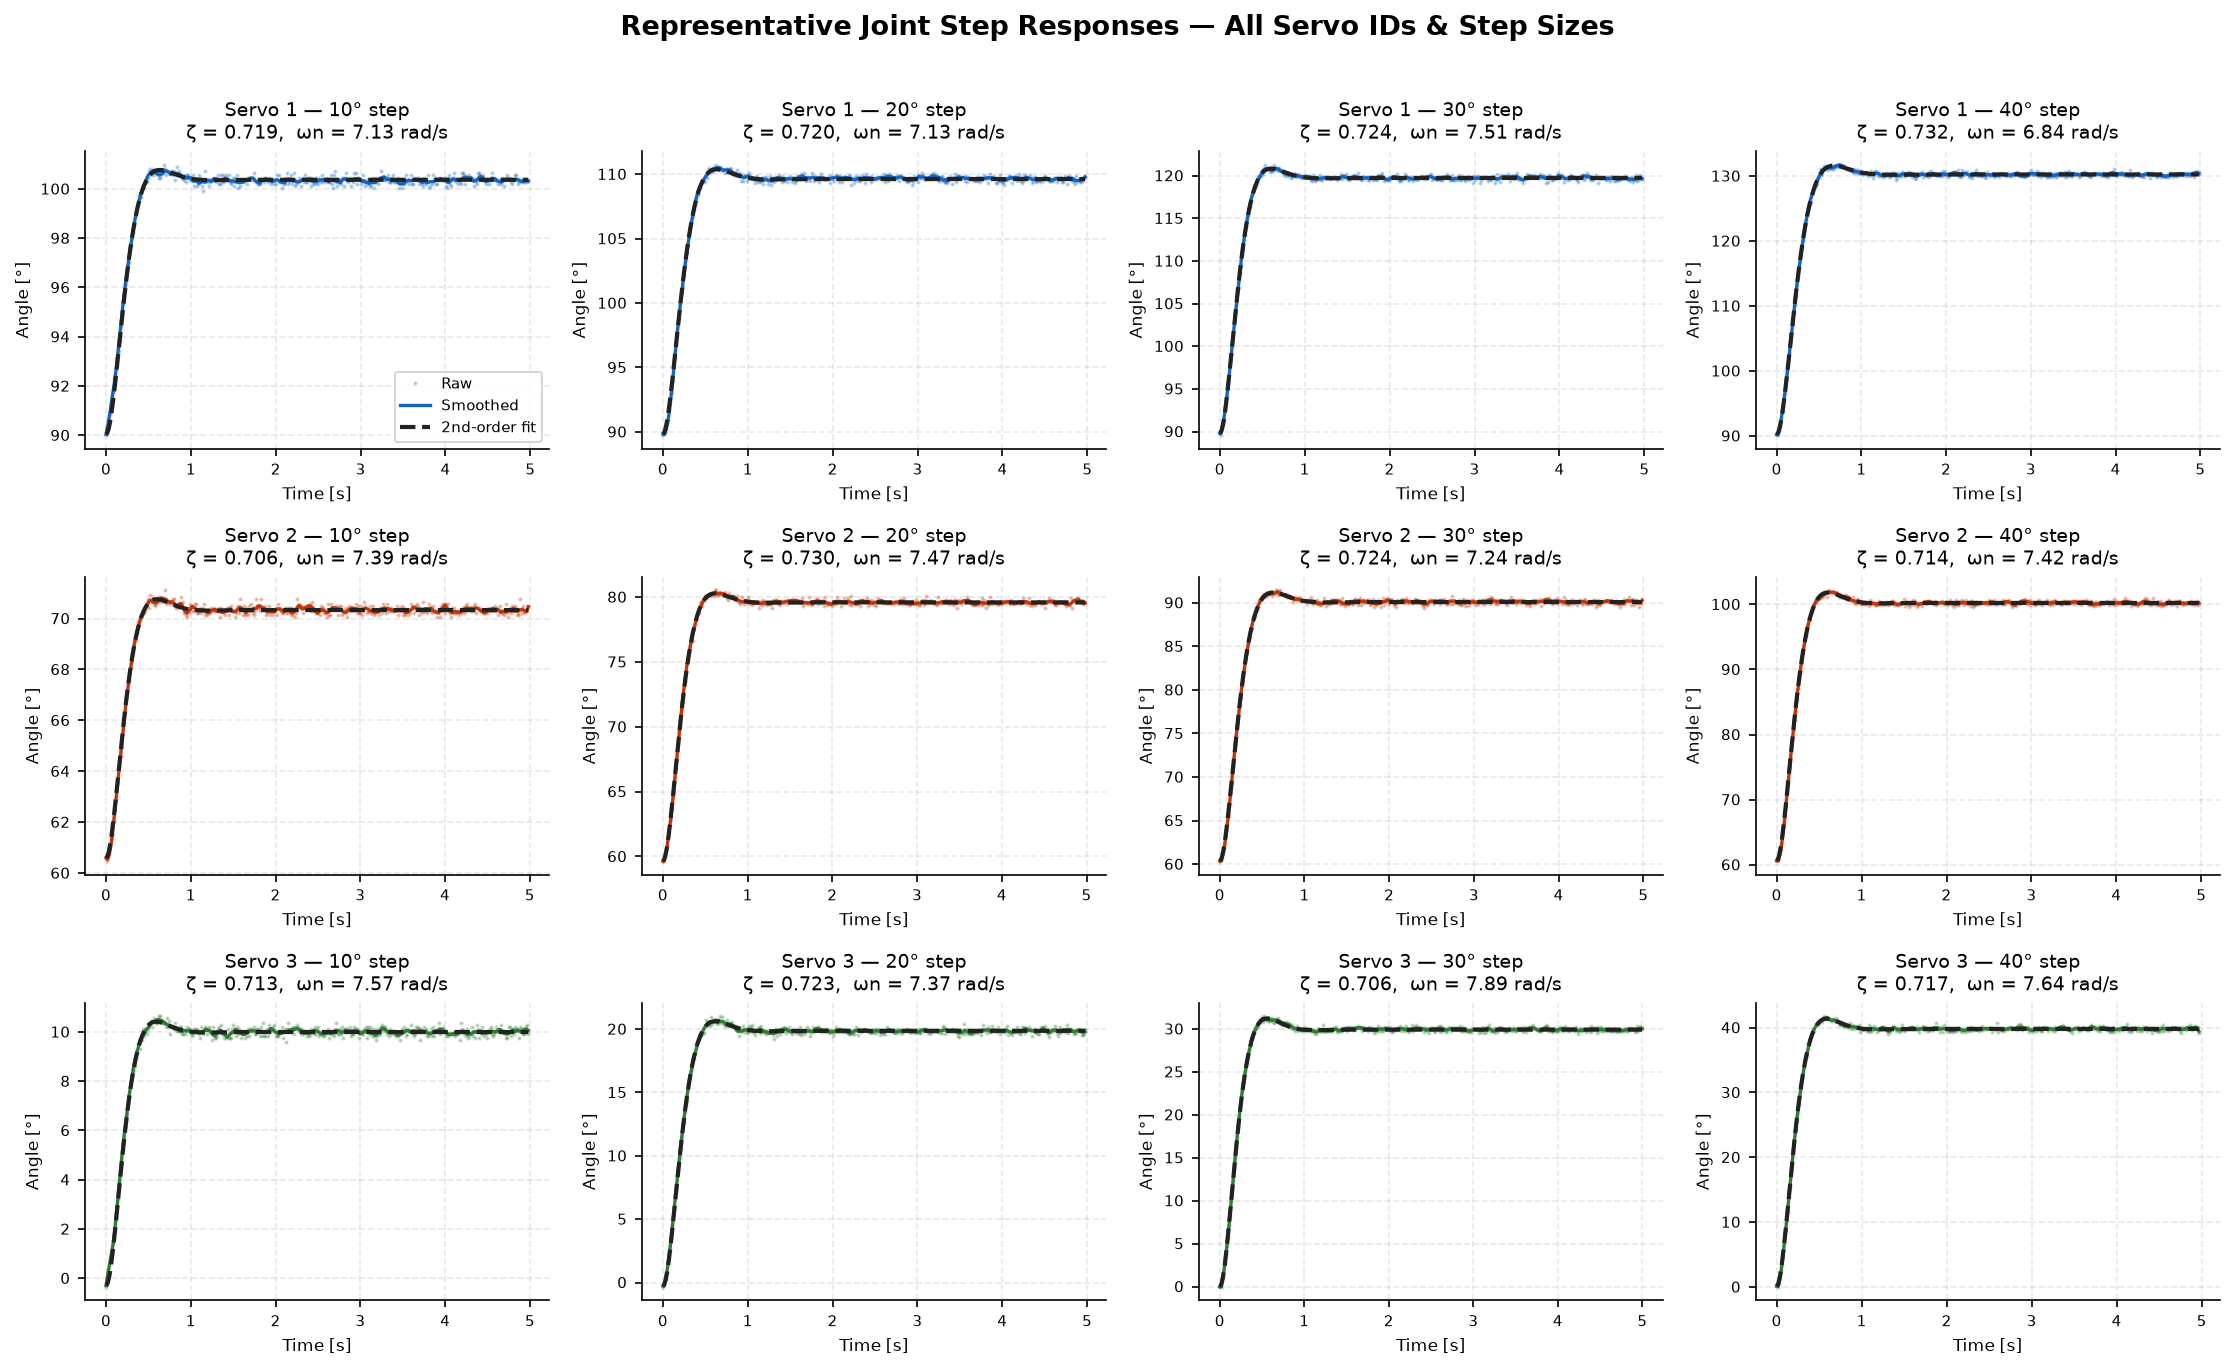
\includegraphics[width=\textwidth]{Figures/report/joint_step_responses.png}
  \caption{Representative step responses with second-order fits.}
\end{subfigure}
\hfill
\begin{subfigure}[b]{0.37\textwidth}
  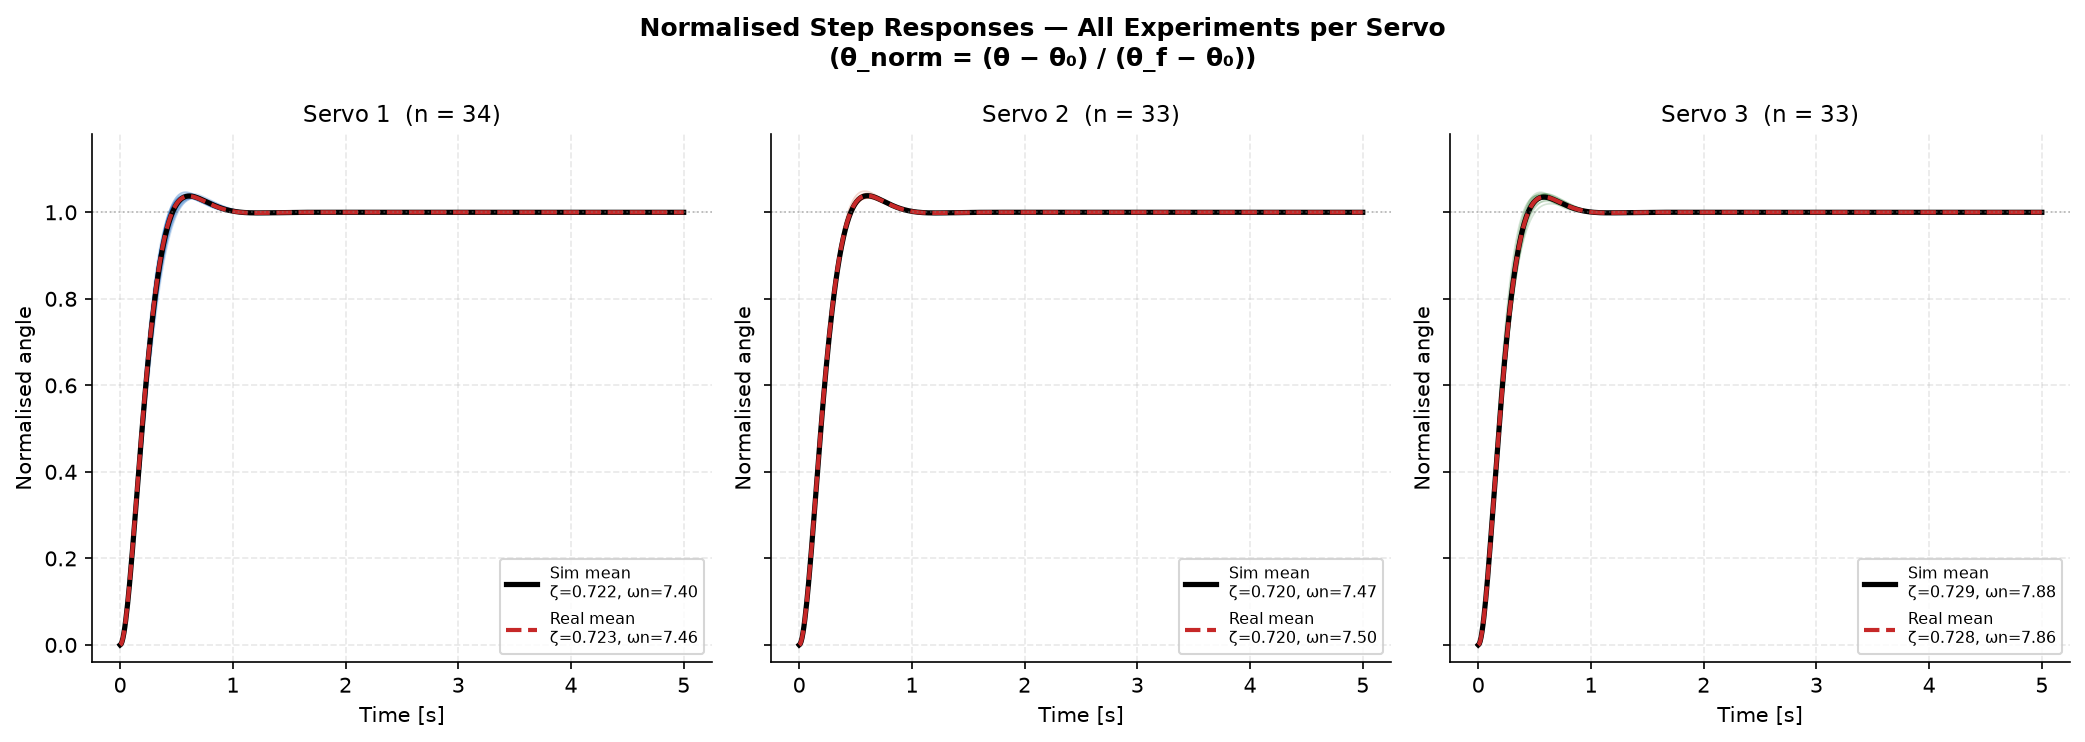
\includegraphics[width=\textwidth]{Figures/report/joint_normalized_fits.png}
  \caption{Normalised fit overlay.}
\end{subfigure}
\caption{Joint identification: step-response fit, free-oscillation decay, and frequency response.}
\label{fig:mech_joint_identification_placeholder}
\end{figure}

\subsubsection{TorqueNADO Motor Parameter Identification}\label{sec:motorid}
The DC drive motor follows
\begin{equation}\label{eq:motoreq}
V=Ri+L\frac{\mathrm di}{\mathrm dt}+K_e\omega,\qquad J\dot\omega=K_ti-b\omega-\tau_L.
\end{equation}
\textbf{Scenario 1 (no-load steady state):} $V=Ri+K_e\omega$ solved by least squares $\hat{\boldsymbol\theta}=(\Phi^\top\Phi)^{-1}\Phi^\top\mathbf{y}$ gives $R=\mechSI{16}{\Omega}$, $K_e=0.013178~\mathrm{V/(rad/s)}$ ($R^2>0.9$).
\textbf{Scenario 2 (coast-down):} $\omega=\omega_0e^{-t/\tau}$, $\ln\omega=\ln\omega_0-t/\tau$ gives $\tau=\mechSI{1.1336}{s}$, $b/J=1/\tau=\mechSI{0.8819}{s^{-1}}$.
\textbf{Scenario 3 (step):} $J\dot\omega\approx K_ti\Rightarrow J=K_ti/\dot\omega=\mechSI{0.001}{kg.m^2}$, then $b=J(b/J)\approx\mechSI{8.82e-4}{N.m.s}$.
\textbf{Scenario 4 (low duty):} $V\approx Ri$ re-confirms $R$.

\begin{table}[htbp]\centering
  \caption{Identified TorqueNADO motor parameters.}\label{tab:motor}
  \small\setlength{\tabcolsep}{5pt}
  \begin{tabular}{@{}llll@{}}
    \toprule
    Parameter & Symbol & Value & Source\\\midrule
    Winding resistance & $R$ & $\mechSI{16}{\Omega}$ & No-load; low-duty\\
    Back-EMF constant & $K_e$ & $0.013178~\mathrm{V/(rad/s)}$ & No-load regression\\
    Torque constant & $K_t$ & $\approx K_e=0.013178~\mathrm{N\,m/A}$ & DC-machine identity\\
    Friction/inertia & $b/J$ & $\mechSI{0.8819}{s^{-1}}$ & Coast-down\\
    Rotor inertia & $J$ & $\mechSI{0.001}{kg.m^2}$ & Step response\\
    Viscous friction & $b$ & $\approx\mechSI{8.82e-4}{N.m.s}$ & $b=J\cdot b/J$\\
    Inductance & $L$ & $\mechSI{0.001}{H}$ & Datasheet/fit\\
    \bottomrule
  \end{tabular}
\end{table}

The electrical time constant $\tau_e=L/R=\mechSI{6.25e-5}{s}\ll\tau=\mechSI{1.1336}{s}$, so inductance is negligible and the motor acts as a torque source $\tau\approx K_ti$ under a fast inner current loop.

\begin{figure}[!htbp]
\centering
\begin{subfigure}[b]{0.48\textwidth}
  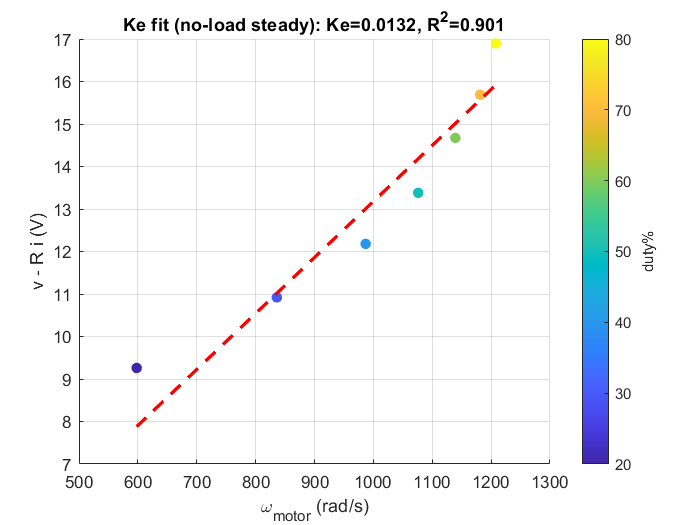
\includegraphics[width=\textwidth]{Figures/report/mech_motor_id1.png}
  \caption{Coast-down and no-load identification (Scenario 1 \& 2).}
\end{subfigure}
\hfill
\begin{subfigure}[b]{0.48\textwidth}
  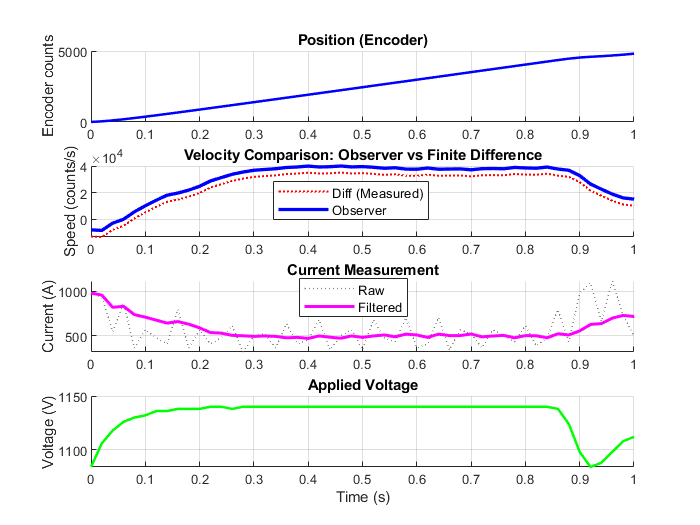
\includegraphics[width=\textwidth]{Figures/report/mech_motor_id2.png}
  \caption{Step and low-duty electrical regression (Scenario 3 \& 4).}
\end{subfigure}
\caption{Motor identification: coast-down decay and no-load electrical regression.}
\label{fig:mech_motor_identification_placeholder}
\end{figure}

\subsubsection{Isaac Sim Validation}\label{sec:isaac}
The URDF was imported into Isaac Sim as a physics articulation carrying the CAD inertials and SDF collisions. Joint limits, the passive-wrist coupling, and stable SDF contacts were verified. Static torques reproduced $G(\mathbf{q})$ \eqref{eq:G}, and acceleration responses matched $M(\mathbf{q})$ \eqref{eq:M}. The kinematics matched \texttt{works/} to numerical precision: FK to $5.6\times10^{-17}\,\mathrm{m}$, analytic IK to a worst-case $\mechSI{0.21}{mm}$ over $\sim$4500 targets with no failures, and the firmware port to $\sim1.7\times10^{-13}\,\mathrm{mm}$. These residuals confirm that the real arm, the planning model, and the twin agree to within numerical precision.

\begin{figure}[!htbp]
\centering
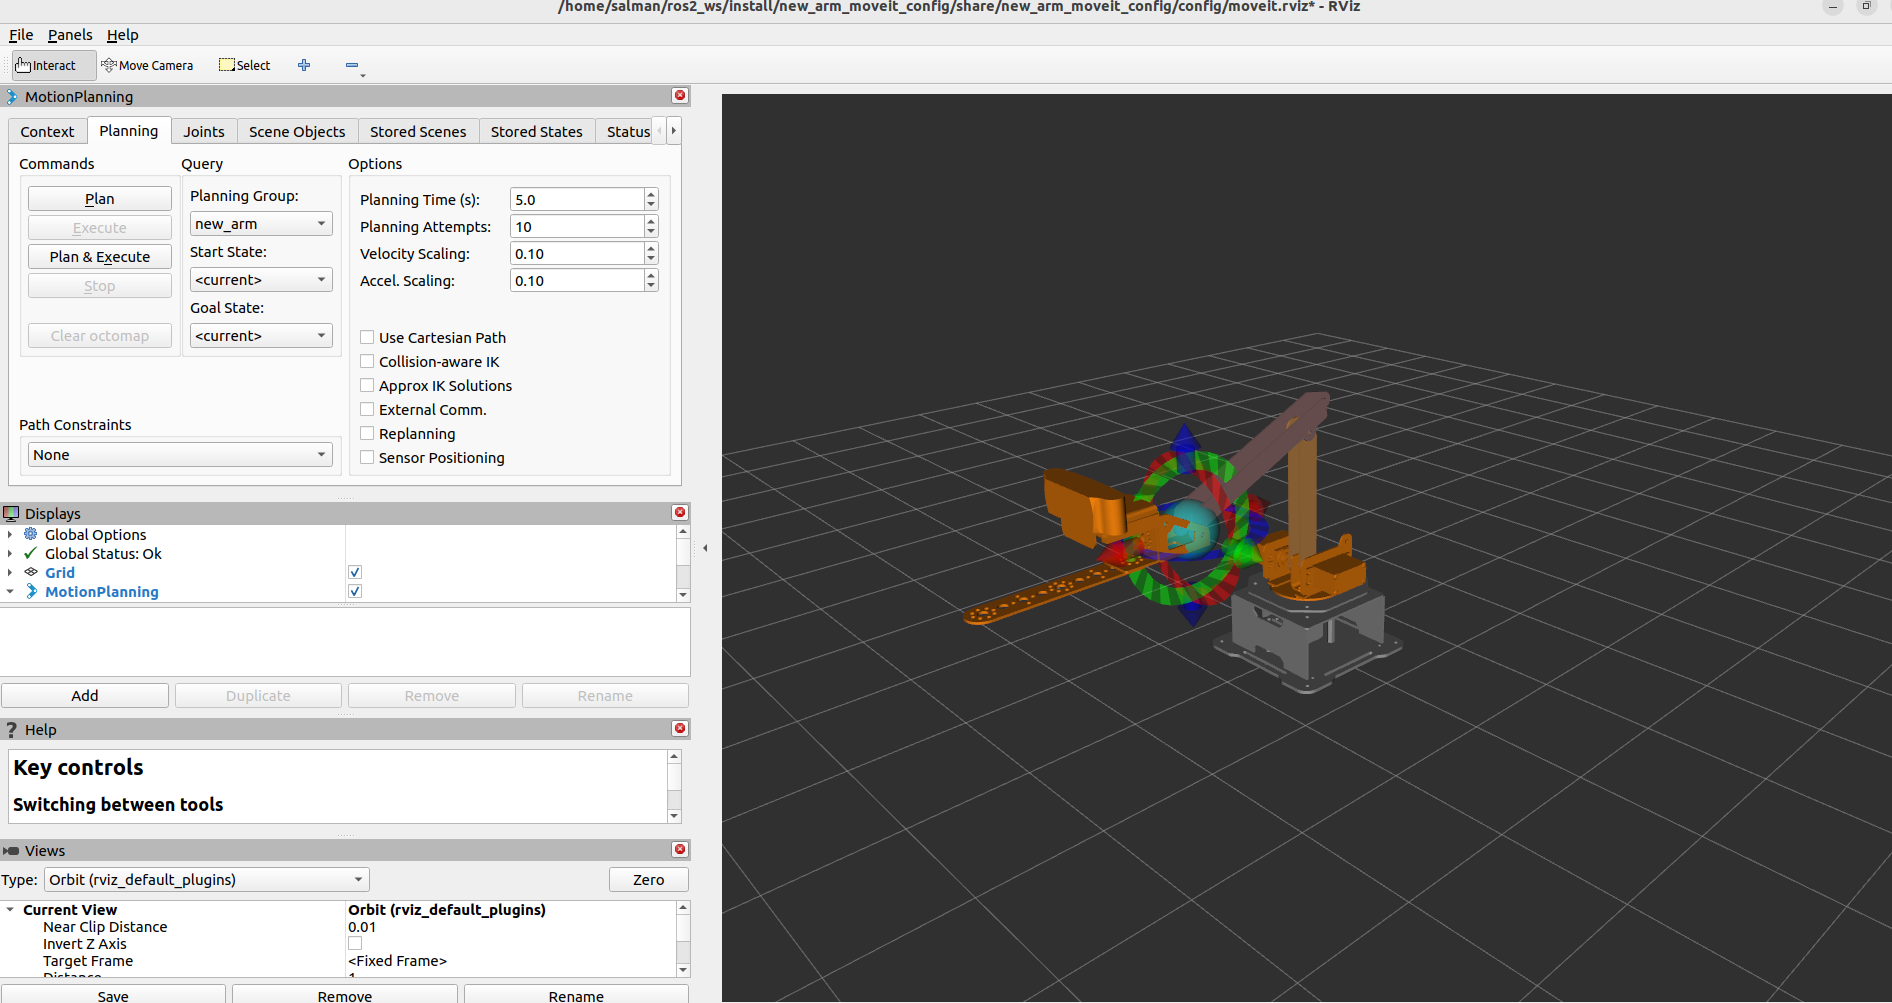
\includegraphics[width=0.88\textwidth]{Figures/report/mech_digital_twin.png}
\caption{Validation of the digital twin against the hardware and the reference kinematics.}
\label{fig:mech_digital_twin_validation_placeholder}
\end{figure}




%========================electrical_design===========================
% Electrical-design fragment for insertion after the Task subsection.

\subsection{Electrical Design and Low-Level Control}
\label{sec:electrical_design}

The robot has two actuation domains. The differential-drive base uses brushed DC gear motors and a dedicated drive controller. The 3-DoF manipulator uses Hiwonder serial-bus servos controlled through an ESP32. Both are supplied from one 12~V lithium-polymer battery using a star power distribution. The drive controller is connected directly to the battery through its barrel jack, so the intermittent motor current follows a short, low-resistance path. A 5~V/3~A buck converter provides a regulated supply for the Raspberry Pi~4 and the USB-powered devices, including the eye-in-hand camera and the ESP32 controller. This separates the logic and sensing supply from motor voltage drops and switching noise. Heavy-gauge wiring and a current-rated connector are used on the motor branch, while lower-current wiring is used for the sensing and signal branch.

\subsubsection{Mobile-base drive electronics and sensing}
\label{sec:electrical_drive}

Two TorqueNADO permanent-magnet DC (PMDC) gear motors with 60:1 gearboxes and output-shaft quadrature encoders drive the base. They are driven through a controller that includes a microcontroller, a dual full-bridge stage, and per-channel sensing. The drive stage is rated at about 10~A continuous per channel over a 12--18~V supply range, with current sensing up to about 30~A peak. It receives PWM velocity commands, reads the encoders, and provides voltage and current telemetry. Through this controller the base exposes one external interface: a velocity command in, with position and electrical feedback out. The encoders provide 360 counts per revolution, or 1440 counts per revolution with four-fold quadrature decoding. This gives approximately $0.125^\circ$ per count at the output shaft. The controller reads the electrical state using an internal voltage divider and a Hall-effect current sensor for each channel. Both measurements are sampled by a 10-bit ADC and feed the motor model and observer described in Section~\ref{sec:electrical_observer}.

\subsubsection{DC-motor model, state-space model, and velocity observer}
\label{sec:electrical_observer}

Each drive motor is represented as a PMDC motor. The parameter values used in the model are $R=16~\Omega$, $L=1~\mathrm{mH}$, $K_e=K_t=0.013178$ ($K_e$ in $\mathrm{V\,s/rad}$, $K_t$ in $\mathrm{N\,m/A}$), $J=10^{-3}~\mathrm{kg\,m^2}$, and $b/J=0.8819~\mathrm{s}^{-1}$:
\begin{equation}
\label{eq:elec_motor}
V=R\,i+L\dot i+K_e\,\omega,\qquad
J\dot\omega=K_t\,i-b\,\omega,\qquad
\dot\theta=\omega .
\end{equation}

With the state vector $\mathbf{x}=[\theta\ \omega\ i]^\top$ and the input $u=V$, the model is written as $\dot{\mathbf{x}}=\mathbf{A}\mathbf{x}+\mathbf{B}u$ and $\mathbf{y}=\mathbf{C}\mathbf{x}$. Only the encoder position $\theta$ and motor current $i$ are measured:
\begin{equation}
\label{eq:elec_state_space}
\mathbf{A}=
\begin{bmatrix}
0&1&0\\
0&-b/J&K_t/J\\
0&-K_e/L&-R/L
\end{bmatrix}
=
\begin{bmatrix}
0&1&0\\
0&-0.882&13.18\\
0&-13.18&-16000
\end{bmatrix},
\qquad
\mathbf{B}=
\begin{bmatrix}
0\\
0\\
1/L
\end{bmatrix}
=
\begin{bmatrix}
0\\
0\\
1000
\end{bmatrix},
\end{equation}
where $\mathbf{C}=[\,\mathbf{e}_1\ \ \mathbf{e}_3\,]^\top$ selects the measured position and current.

The electrical time constant is $\tau_e=L/R=62.5~\mu\mathrm{s}$, while the mechanical time constant is $\tau=J/b=1.13~\mathrm{s}$. Current therefore settles much faster than the mechanical speed. The wheel controller still needs the unmeasured speed $\omega$. A direct finite difference,
$\omega_{\mathrm{diff}}[k]=(\theta[k]-\theta[k-1])/T_s$, amplifies encoder quantization and measurement noise, especially at low speed. A minimum-order observer is used instead. Since two of the three states are measured, only $\omega$ is estimated.

Let $\mathbf{x}_a=[\theta\ i]^\top$ denote the measured states and $x_b=\omega$ the unmeasured state. Using the auxiliary state $\eta=\hat{\omega}-\mathbf{K}_o\mathbf{x}_a$ gives
\begin{equation}
\label{eq:elec_observer}
\begin{gathered}
\dot{\hat{\eta}}=\hat{A}\,\hat{\eta}
+\hat{\mathbf{B}}\,\mathbf{x}_a+\hat{F}\,u,
\qquad
\hat{\omega}=\hat{\eta}+\mathbf{K}_o\mathbf{x}_a,\\
\hat{A}=A_{bb}-\mathbf{K}_o\mathbf{A}_{ab},
\qquad
\hat{\mathbf{B}}=\hat{A}\mathbf{K}_o+\mathbf{A}_{ba}
-\mathbf{K}_o\mathbf{A}_{aa},
\qquad
\hat{F}=B_b-\mathbf{K}_o\mathbf{B}_a .
\end{gathered}
\end{equation}

The observer error follows $\dot e_b=(A_{bb}-\mathbf{K}_o\mathbf{A}_{ab})e_b$, so its single pole is set directly through $\mathbf{K}_o$. Placing this pole at $\mu=-20$ gives the gain $\mathbf{K}_o=[\,0.1095\ \ {-}1.4425\,]$, and hence $\hat{A}=-20$, $\hat{\mathbf{B}}=[-2.19\ \ {-}2.30\times10^{4}]$, and $\hat{F}=1442.5$. The corresponding observer time constant is $50~\mathrm{ms}$, with an approximate $0.25~\mathrm{s}$ settling time. The estimate avoids the noise amplification caused by direct differentiation.

\subsubsection{Discrete implementation and speed control}
\label{sec:electrical_control}

Estimation and speed control run at $T_s=20~\mathrm{ms}$, or 50~Hz. The observer in \eqref{eq:elec_observer} is discretized using forward Euler:
\[
\hat{\eta}[k+1]=\hat{\eta}[k]+T_s\left(
\hat{A}\hat{\eta}[k]+\hat{\mathbf{B}}\mathbf{x}_a[k]+\hat{F}V[k]\right).
\]
The armature-current measurement is affected by high-frequency PWM and electromagnetic noise, so it is filtered with a first-order exponential moving average of cut-off frequency $f_c$; the wheel speed is then regulated by a discrete PID law acting on the speed error:
\begin{equation}
\label{eq:elec_pid}
i_{\mathrm{filt}}[k]=\alpha i_{\mathrm{raw}}[k]
+(1-\alpha)i_{\mathrm{filt}}[k-1],
\qquad
f_c=\frac{\alpha f_s}{2\pi(1-\alpha)};
\qquad
u[k]=K_pe[k]+K_iT_s\sum_{j=0}^{k}e[j]
+K_d\frac{e[k]-e[k-1]}{T_s},
\end{equation}
where $e[k]=\omega_{\mathrm{ref}}[k]-\hat{\omega}[k]$. The PWM command is clamped, and the integrator is held when saturation occurs to prevent windup.

The body command is converted to wheel-speed references through the inverse differential-drive relation. For track width $L_t$ and wheel radius $r_d$,
\[
\omega_{R,\mathrm{ref}}=
\frac{v+\tfrac{1}{2}L_t\omega_z}{r_d},
\qquad
\omega_{L,\mathrm{ref}}=
\frac{v-\tfrac{1}{2}L_t\omega_z}{r_d}.
\]
At a small computational cost, the observer yields a lower-noise speed estimate with an explicitly selectable convergence rate.

\subsubsection{Manipulator actuation and embedded bridge}
\label{sec:electrical_arm}

The three active joints use Hiwonder serial-bus servos. The fourth wrist joint is passive and is mechanically leveled. Each active servo includes a local controller, a magnetic encoder, and an internal position loop. The servo receives a target position and a movement time, then reports position, input voltage, and temperature. The three servos share a half-duplex TTL bus at 115200~baud using 8N1 framing and IDs 1--3. A position change of 1000 pulses corresponds to $240^\circ$, giving
\[
\frac{\mathrm{d}p}{\mathrm{d}\theta}
=
\frac{1000}{240}\frac{180}{\pi}
=
238.7324
\quad \text{pulses/rad}.
\]

The ESP32 acts as a bridge between the host computer and the servo bus. A USB serial link carries arm commands from the Raspberry Pi~4 to the ESP32. The ESP32 drives the servo bus through a dedicated hardware UART. Because the bus is half-duplex, the ESP32 switches its transceiver between transmit and receive states before each command and before each reply. The host sends the command vector \texttt{[p1,p2,p3,time\_ms]}. The ESP32 clamps the commands, sends timed moves to the servos, and streams read-back positions at 20~Hz. Each bus frame begins with \texttt{0x55 0x55}, followed by the servo ID, length, command, payload, and checksum.

The host converts between joint angles and servo pulses using
\begin{equation}
\label{eq:elec_joint_map}
p_i=s_i\theta_i+o_i,
\qquad
\theta_i=\frac{p_i-o_i}{s_i},
\qquad
\theta_4=2\pi-\frac{\pi}{2}-\theta_{\mathrm{sh}}-\theta_{\mathrm{el}},
\end{equation}
where the pulse-scale vector is
$s=[238.73,\ {-}238.73,\ 238.73]$~pulses/rad and the offset vector is
$o=[625,\ 875,\ 500]$. The sign of each scale term accounts for the joint mounting direction. The pulse-angle mapping is based on the manufacturer relation and must be checked on the physical arm by commanding known angles, reading the reported pulses, and fitting the scale and offset values.

\subsubsection{Simulation-to-hardware signal path and layered safety}
\label{sec:electrical_sim_to_real}

The command path is the same in simulation and on the physical arm up to the servo bus. A target produced by the reinforcement-learning policy or a planner is expressed in joint radians, converted to pulses using \eqref{eq:elec_joint_map}, clamped, and sent to the ESP32. The ESP32 writes the timed move to the bus, and each servo closes its own position loop. Feedback returns in the opposite direction. Read-back pulses are converted to joint angles, the passive-wrist relation is applied, and the joint state is sent to the host at 20~Hz. If feedback is temporarily unavailable, the bridge echoes the previous command, so the joint-state stream remains continuous.

The base path is shorter. The host sends a body-velocity command, the differential-drive relation produces the wheel references, and the base controller regulates the motor speed while returning encoder and electrical telemetry. Safety is implemented in four layers. The host rejects targets outside the allowed range. The ESP32 clamps every pulse to the valid interval. The servos enforce their own angle, voltage, and temperature limits. Finally, the base controller uses current limits to bound motor torque independently of the PWM duty cycle.




%========================software_design===========================
% Paste this file after the Task subsection in the System Design section.
% It uses packages already loaded by main.tex: amsmath, graphicx, booktabs,
% array, xcolor, float, tikz, and hyperref.

% ---- software architecture diagram styles ----
\definecolor{cproc}{RGB}{225,235,250}
\definecolor{cnode}{RGB}{223,242,228}
\definecolor{ctopic}{RGB}{253,240,221}
\definecolor{cdata}{RGB}{238,238,242}
\definecolor{clayer}{RGB}{244,247,252}
\tikzset{
  box/.style   ={draw=blue!40, rounded corners=2pt, align=center, font=\small,
                 inner sep=4pt, minimum height=8mm, fill=cproc},
  proc/.style  ={box},
  data/.style  ={draw=gray!55, align=center, font=\small, inner sep=4pt,
                 minimum height=7mm, fill=cdata, rounded corners=1pt},
  rnode/.style ={draw=green!45!black, rounded corners=8pt, align=center,
                 font=\footnotesize, inner sep=4pt, minimum height=7mm, fill=cnode},
  topic/.style ={draw=orange!60!black, align=center, font=\scriptsize,
                 inner sep=3pt, minimum height=5.5mm, fill=ctopic, rounded corners=1pt},
  state/.style ={draw=blue!50, rounded corners=5pt, align=center, font=\small,
                 inner sep=4pt, minimum height=8mm, fill=cproc},
  layer/.style ={draw=blue!35, rounded corners=3pt, inner sep=7pt, fill=clayer},
  arr/.style   ={-{Latex[length=2.2mm]}, semithick, blue!55!black},
  darr/.style  ={-{Latex[length=2.2mm]}, semithick, dashed, gray!60!black},
  lbl/.style   ={font=\scriptsize, fill=white, inner sep=1.5pt},
}

\subsection{Software Architecture and System Integration}\label{sec:software_architecture}

The mechanical and electrical chapters established a robot that can move and be commanded; this chapter describes the software that decides \emph{what} to command. From a single RGB-D camera, a low-cost mobile base, and a microcontroller-driven arm, the system must build a map of a room it has never seen, locate itself within that map while moving, drive to a charging station, find the socket on the wall, bring a 3-DoF arm to it, and insert a plug. The software architecture is what turns that collection of devices into one autonomous agent. The chapter is organized by data flow: each layer is introduced through the information it consumes and produces, because the interfaces between modules are what make the system comprehensible and testable, and only then are the algorithms described. Every mathematical model is tied to the concrete signal it operates on inside the robot.

\subsubsection{Software Architecture Overview}\label{sec:overview}

The software is organized as six layers, each depending only on the interfaces exposed by the layer beneath it. The layering bounds the dependencies of every module, so that a change in the camera driver cannot ripple into the mission logic, and it lets each layer be validated in isolation (Section~\ref{sec:validation}) before the full pipeline is closed. From the bottom up, the \emph{Hardware Abstraction Layer} hides the electrical interfaces behind ROS~2 topics and services. The \emph{Sensor and Perception Layer} converts raw images into synchronized, calibrated streams. The \emph{Localization and Mapping Layer} turns those streams into a real-time pose estimate (dynamic visual SLAM) and a reconstructed volumetric model of the environment (nvblox). The \emph{Navigation Layer} (Nav2) plans and executes collision-free motion of the base toward a goal. The \emph{Manipulation Layer} drives the arm to a target socket pose. The \emph{Mission Management Layer} sequences the whole charging operation as a finite-state machine and supervises failure recovery.

The independence is concrete: the base controller on the Pi consumes \texttt{/cmd\_vel} and returns wheel odometry; the arm controller consumes joint targets and returns joint states; neither knows how those messages were produced. This is what allows the navigation stack to be developed and tested entirely on the laptop, with the Pi bridges substituted by simulated equivalents, before the physical base is attached.

\subsubsection{Hardware Abstraction Layer}\label{sec:hal}

The Hardware Abstraction Layer (HAL) is the boundary at which physical signals become ROS~2 messages; no module above it touches a USB endpoint, serial port, or pulse train directly. The \textbf{Intel RealSense D435i} is driven by the \texttt{realsense2\_camera} node, which wraps the \texttt{librealsense2} SDK and the kernel UVC stack; it publishes the rectified infrared pair at $848\times480$ for visual odometry, the aligned depth and color at $1280\times720$ for mapping, and the IMU stream, all over USB~3.0. The \textbf{ESP32} arm microcontroller runs a micro-ROS client and joins the network through the \texttt{micro\_ros\_agent}, which bridges its serial link (115200~baud) into DDS. The \textbf{TETRIX PRIZM controller} on the Pi is exposed by the \texttt{prizm\_interface} node, which accepts \texttt{/cmd\_vel} and returns wheel odometry. The \textbf{TorqueNADO motors} are not addressed individually: PRIZM closes their current and velocity loops in firmware and accepts wheel-velocity setpoints, and the \textbf{wheel encoders} it reads surface as the published odometry. The \textbf{arm servos} are Hiwonder serial-bus servos whose position loops run inside the servos themselves; the ESP32 issues bus packets, and the host converts joint angles to servo pulses. The firmware details of both the PRIZM and the servo bus are given in the electrical-design subsection.

Two design principles run through the HAL. Device \emph{drivers} own the protocol and timing of each device, while thin \emph{ROS wrappers} expose it as typed messages. And the wheel kinematics that convert a commanded body twist $(v,\omega)$ into left and right wheel speeds,
$$
\omega_L=\frac{v-\tfrac{b}{2}\,\omega}{r_w},\qquad
\omega_R=\frac{v+\tfrac{b}{2}\,\omega}{r_w},
$$
with wheel radius $r_w$ and track width $b$ (Section~\ref{meth:sec:dyn}), live in the HAL, so everything above it commands the robot in physical units rather than motor counts.

\subsubsection{Perception Layer}\label{sec:perception}

Raw image and depth frames are not yet usable for geometry. The perception pipeline acquires the RGB and depth images, synchronizes them in time, registers depth into the color frame, and produces the calibrated, time-synchronized RGB-D stream that localization and mapping consume.

Time synchronization matters because the depth image is triangulated from the left and right infrared frames: if the two are captured at different instants, motion corrupts the apparent disparity and the recovered depth. The driver therefore hardware-timestamps each frame, and the pipeline associates only frames whose stamps fall within a tight window. Depth-to-color registration reprojects each depth pixel into the color camera, so that a color pixel and its metric depth refer to the same scene point.

The geometric core of the layer is the pinhole camera model, which relates a 3-D point in the camera frame to its pixel by dividing by depth (so distant objects subtend fewer pixels) through the focal lengths and principal point---the four \emph{intrinsic parameters}, delivered to every node on the \texttt{camera\_info} topic. Inverting the model back-projects a depth pixel of measured range into a metric 3-D point for mapping, and the \emph{extrinsic} rigid transform $T_{\text{cam}}^{\text{base}}\in SE(3)$ places the camera on the robot; lens distortion is removed before projection so the linear model holds. The projection, back-projection, and intrinsic/extrinsic definitions are derived in Section~\ref{meth:sec:perception} (Eqs.~\eqref{meth:eq:projection}--\eqref{meth:eq:backproj}).

These transforms are organized by the \textbf{TF tree}, the system's single source of truth for spatial relationships. The dynamic visual SLAM backend publishes the \texttt{map}$\to$\texttt{odom} edge, while the \texttt{prizm\_interface} node publishes \texttt{odom}$\to$\texttt{base\_link} from wheel odometry; the full transform algebra is given in Section~\ref{meth:sec:perception}.

Every measurement in the robot --- a detected socket pixel, a mapped voxel, a planned waypoint --- is ultimately a query on this tree of chained homogeneous transforms.

\subsubsection{Localization Layer}\label{sec:localization}

Localization is provided by a custom \textbf{dynamic visual SLAM} pipeline (Section~\ref{meth:sec:slam}), a GPU-accelerated estimator that consumes the registered RGB-D stream together with the IMU and a wheel-odometry prior. Its backend publishes the \texttt{map}$\to$\texttt{odom} transform and an odometry message on \texttt{/visual\_slam/tracking/odometry}, on which the mapper and navigator both depend; the \texttt{odom}$\to$\texttt{base\_link} edge is supplied separately by the wheel-odometry bridge. On this hardware it tracks at the full 30\,Hz of the camera, with a GPU pose-update time of about 0.5\,ms.

Internally, the pipeline follows the standard visual-SLAM sequence: it detects and matches features, recovers the camera pose from the 3-D landmarks and their 2-D observations by solving the Perspective-$n$-Point (PnP) problem, rejects wrong correspondences with RANSAC, and then refines pose and landmarks together by sliding-window bundle adjustment that minimizes the reprojection error under a robust loss. Poses are elements of $SE(3)$, with the rotation transmitted as a unit quaternion that avoids gimbal lock; composing them is the chained matrix multiplication that the TF tree of Section~\ref{sec:perception} performs. The reprojection-error, PnP, bundle-adjustment, $SE(3)$, and RANSAC formulations are derived in Section~\ref{meth:sec:slam}.

\subsubsection{Mapping Layer}\label{sec:mapping}

While the dynamic visual SLAM answers \emph{where am I}, \textbf{nvblox} answers \emph{what is around me}. It fuses the registered depth frames into a volumetric model in the \texttt{odom} frame and exports the obstacle map the navigator needs: a colored surface mesh at roughly 14\,Hz and a 2-D distance slice for navigation at 10\,Hz.

The model is a \textbf{truncated signed distance field (TSDF)}: space is divided into voxels, each storing the signed distance from its center to the nearest measured surface (negative behind, positive in front), truncated to a band $\pm\tau$. Each depth frame updates the voxels by confidence-weighted averaging, so many noisy single-frame measurements converge to one stable estimate and spurious readings are averaged away; a voxel seen many times becomes firm, while one far from the camera or deep behind the truncation band, where depth noise grows, carries little weight. The visible surface is the zero-crossing $D(v)=0$, extracted as a mesh by marching cubes.

For planning, the TSDF is converted into a \textbf{Euclidean signed distance field (ESDF)}, in which every voxel stores the true Euclidean distance to the nearest obstacle, so its value is the clearance and its gradient $\nabla E$ points away from the nearest obstacle---exactly what a planner needs to know how far the robot can move before a collision and in which direction clearance increases. nvblox exports a horizontal slice in a band above the floor ($0.10$--$0.60$\,m) as the 2-D cost layer Nav2 consumes; because the system maps dynamic scenes, this slice is published as a \emph{combined} static-plus-dynamic map, so moving obstacles appear and then clear once they leave. The TSDF fusion update and the ESDF distance transform are given in Section~\ref{meth:sec:nvblox}.

\subsubsection{Navigation Layer}\label{sec:navigation}

\textbf{Nav2} plans and executes the motion of the base. It takes a goal pose, the robot's current pose, and the obstacle map, computes a path, and tracks it by emitting velocity commands, while a behavior tree supervises and triggers recovery. In this system Nav2 is configured \emph{without} a static map server and \emph{without} AMCL: the dynamic visual SLAM and the wheel-odometry bridge already supply the full \texttt{map}$\to$\texttt{odom}$\to$\texttt{base\_link} transform chain, and nvblox already supplies the obstacle costmap, so Nav2 consumes those products directly.

The \textbf{global planner} searches the global costmap for a complete collision-free path. The \textbf{local planner} (controller server) tracks that path over a short horizon, reacting to unforeseen obstacles, and produces the body twist. The \textbf{behavior-tree navigator} encodes the plan-then-follow-else-recover logic as an inspectable tree, and the \textbf{recovery server} provides corrective behaviors (spin, back up, wait). Finally, the \textbf{velocity smoother} limits the acceleration of the commanded twist before it reaches the motors.

The motion model is the \textbf{differential-drive (unicycle) kinematics}: the base can only move along its current heading and rotate about its center, the nonholonomic constraint every Nav2 controller must respect, which is why the local planner reasons in $(v,\omega)$ rather than in free Cartesian velocity. The PRIZM wheel odometry integrates this model from wheel speeds, and the dynamic visual SLAM corrects its drift. \textbf{Path tracking} chooses $(v,\omega)$ so the predicted trajectory stays on the global path while remaining in free space: the controller rolls out candidate command sequences, scores each by distance to the path and clearance read from the costmap, and applies the best, binding the costmap, the kinematic model, and the command into one optimization. The \textbf{costmaps} are the inflated obstacle grids derived from the nvblox slice, each obstacle cell expanded by the robot radius plus a decaying margin so the planners can treat the robot as a point. The unicycle kinematics and their discrete odometry integration are stated in Section~\ref{meth:sec:nav}.

\subsubsection{Socket Detection and Pose Estimation}\label{sec:socket}

Once the base reaches the charging station, perception narrows from locating the station to locating the socket on it. Socket perception is staged. A coarse estimate from the base-mounted RealSense detects the socket and, using its depth and the camera-to-base extrinsics, places the socket's six-degree-of-freedom pose in the base frame to guide the final approach and base repositioning. A fine estimate from the eye-in-hand camera then drives the close-range alignment and insertion.

The coarse detection combines a classical color-segmentation routine, which exploits the high-contrast geometry of the socket face, with a learned CenterPose keypoint detector, which regresses the socket's projected bounding cuboid. Both yield image-plane locations; their depth is read from the registered depth frame, and the camera model of Section~\ref{sec:perception} converts them into the socket pose in the camera frame.

The output the manipulation layer needs is the socket pose in the \emph{robot} frame, obtained by \textbf{transformation composition} along the TF tree:
$$
T^{\text{base}}_{\text{socket}} = T^{\text{base}}_{\text{cam}}\;T^{\text{cam}}_{\text{socket}}.
$$
Because the camera is mounted on the arm's end-effector, $T^{\text{base}}_{\text{cam}}$ is itself a function of the current joint angles through the forward kinematics of the mechanical-design subsection, so the full \textbf{coordinate conversion} is
$$
T^{\text{base}}_{\text{socket}} = T^{\text{base}}_{\text{ee}}(\boldsymbol{\theta})\;T^{\text{ee}}_{\text{cam}}\;T^{\text{cam}}_{\text{socket}},
$$
chaining the FK transform, the rigid eye-in-hand offset, and the measurement. \textbf{Error propagation} through this chain sets the achievable insertion accuracy: if the camera-frame pose has covariance $\Sigma_{\text{cam}}$, the base-frame covariance is, to first order,
$$
\Sigma_{\text{base}} = J\,\Sigma_{\text{cam}}\,J^\top,\qquad J=\frac{\partial T^{\text{base}}_{\text{socket}}}{\partial T^{\text{cam}}_{\text{socket}}},
$$
so a rotational error in the mount or a depth error in the measurement is amplified by the lever arm of the arm. This is precisely why the eye-in-hand camera performs the \emph{final} alignment from close range, where $\Sigma_{\text{cam}}$ is smallest; at that range the endgame uses the lighter two-hole bearing (image-based visual servoing) representation rather than a full 6-DoF pose, as detailed in Section~\ref{meth:sec:manip:vision}.

\subsubsection{Manipulation Layer}\label{sec:manipulation}

The manipulation layer converts a target socket pose into physical motion of the arm: it solves the inverse kinematics for the joint angles that bring the plug to a pre-insert pose at the socket, generates a smooth trajectory, and streams it to the ESP32. The learned policy of Section~\ref{sec:rl} then performs the final alignment and insertion.

The kinematic models were derived in the Mechanical chapter and are reused unchanged here in their software role. \textbf{Forward kinematics} (Section~\ref{sec:fk}) predicts where the plug currently is from the joint angles. \textbf{Inverse kinematics} (Section~\ref{sec:ik}) is what the socket pose triggers: it returns the base yaw and the shoulder and elbow angles for the target, with the elbow-up branch chosen for clearance. The \textbf{Jacobian} (Section~\ref{sec:jac}) relates joint rates to plug velocity and, through its determinant, warns of the near-straight-elbow singularities, keeping the approach well-conditioned. \textbf{Workspace constraints}---the reachable shell $|L_2-L_3|\le D\le L_2+L_3$---are checked before motion, so an unreachable socket is rejected rather than attempted.

\textbf{Trajectory generation} turns the single IK target into a time-parameterized path, interpolating each joint from $\theta(0)$ to $\theta(T)$ with a \textbf{minimum-jerk} profile,
$$
\theta(t)=\theta(0)+\big(\theta(T)-\theta(0)\big)\big(10s^3-15s^4+6s^5\big),\qquad s=t/T,
$$
whose zero velocity and acceleration at both endpoints give a smooth start and stop the servos can follow without overshoot. This \textbf{joint-space planning} is appropriate because the task is to reach a pose, not to follow a Cartesian contour, and joint-space interpolation is both cheaper and free of the singularities a straight-line Cartesian path can cross. The waypoints are streamed to the ESP32 over micro-ROS, converted to servo pulses by the host affine calibration of the electrical-design subsection, and executed by the servos' internal loops, with returned joint states closing the loop.

\subsubsection{Reinforcement-Learning Layer}\label{sec:rl}

The geometric pipeline aligns the plug to the \emph{estimated} socket pose, but the final millimeters are limited by residual estimation error and the unmodeled contact between plug and socket. The reinforcement-learning layer closes this residual with a policy that observes the alignment error and outputs small joint corrections, learned in simulation and transferred to the real arm. The implemented algorithm is \textbf{Proximal Policy Optimization (PPO)}, which performs the final alignment and insertion (Section~\ref{meth:sec:manip:rl}). \textbf{Soft Actor-Critic (SAC)}, an off-policy actor-critic method whose entropy regularization makes it sample-efficient for continuous control, is a planned future refinement for the contact-rich insertion phase; SAC is retained as a future alternative rather than part of the implemented controller.

The \textbf{observation} is assembled from quantities the rest of the stack already produces---the socket-pose (alignment) error, the end-effector pose, and the joint angles and velocities,
$$
\mathbf{s}=\big[\,\mathbf{e}_{\text{socket}},\;\mathbf{p}_{\text{ee}},\;\boldsymbol{\theta},\;\dot{\boldsymbol{\theta}}\,\big].
$$
The deployed PPO actor uses the same kind of state---hole bearings in place of the explicit pose error, together with the joint angles, velocities, and previous action (Section~\ref{meth:sec:manip:rl}). The \textbf{actions} are bounded joint-position corrections $\mathbf{a}=\Delta\boldsymbol{\theta}$ added on top of the geometric setpoint, so the policy refines rather than replaces the analytic controller and exploration stays safe. The \textbf{reward} rewards alignment and successful insertion while penalizing collision,
$$
r=-w_a\lVert \mathbf{e}_{\text{align}}\rVert + w_s\,\mathbf{1}[\text{inserted}] - w_c\,c_{\text{collision}},
$$
with a dense distance term, a sparse seating bonus, and a contact-force penalty. In the planned SAC variant the policy would instead maximize the \textbf{entropy-regularized return}
$$
J(\pi)=\sum_t \mathrm{E}_{(\mathbf{s}_t,\mathbf{a}_t)\sim\pi}\!\big[\,r(\mathbf{s}_t,\mathbf{a}_t)+\alpha\,\mathcal{H}\big(\pi(\cdot\mid\mathbf{s}_t)\big)\big],
$$
where the temperature $\alpha$ balances exploration against exploitation. A future SAC implementation would use twin critics fitted to a Bellman target and a \textbf{replay buffer} that reuses past transitions.

Because the policy is trained in Isaac Sim and deployed on hardware, it must cross the reality gap. \textbf{Domain randomization} varies the simulator's parameters --- socket pose, friction, lighting, latency, sensor noise --- across episodes, so the policy learns a behavior robust to the very quantities that differ between simulation and the real cell rather than overfitting to one nominal model. \textbf{Sim-to-real transfer} is then deployment of that robustified policy on the physical arm with no change of weights, observing the real state through the same interfaces and acting through the same ESP32 path.

\subsubsection{Mission Management Layer}\label{sec:mission}

The autonomous charging operation is sequenced by a \textbf{finite-state machine (FSM)}: the mission is a chain of distinct phases, each with a clear success condition and a defined response to failure, and an explicit state machine keeps the robot's behavior auditable. This mission-level FSM is distinct from the finer insertion-sequence FSM of Section~\ref{meth:sec:manip:fsm}.

The \textbf{data exchanged} between modules is typed and minimal: the dynamic visual SLAM passes a transform and an odometry message, not images; nvblox passes a 2-D cost slice, not its voxel grid; the socket subsystem passes a single pose; and the IK solver passes a joint-target array. Keeping inter-module messages small bounds the DDS bandwidth and makes each interface easy to record and replay. The \textbf{timing requirements} follow the physical rates of the sensors and actuators. The camera fixes the 30\,Hz ceiling; the SLAM front end and the depth stream feed nvblox at camera rate; the ESDF slice and the Nav2 control loop run at 10\,Hz; and the arm trajectory streams at the servo update rate. The \textbf{synchronization requirements} are strongest at the front of the pipeline, where the infrared pair must be time-aligned for valid depth and depth must be registered to color for valid mapping. They relax toward the back, where the arm reacts to a pose that changes slowly once the base has stopped. The architecture exploits this gradient: tightly synchronized, high-rate perception runs on the GPU laptop with shared-memory transport, while the looser, lower-rate base and arm commands tolerate the small latency of the Wi-Fi and serial links.


\subsubsection{Timing and Computational Analysis}\label{sec:timing}

The system is a soft-real-time pipeline whose rates are set by its sensors and consumers (Table~\ref{tab:timing}).

\begin{table}[H]\centering
\caption{Pipeline rates and resources.}\label{tab:timing}
\small
\begin{tabular}{@{}lll@{}}
\toprule
Stage & Rate / latency & Resource\\\midrule
Camera RGB & 30\,fps (1280$\times$720) & USB 3.0\\
Camera depth & 30\,fps (1280$\times$720) & USB 3.0\\
Stereo IR (depth input) & 30\,fps (848$\times$480) & USB 3.0\\
Dynamic visual SLAM pose update & 30\,Hz, $\sim$0.5\,ms GPU & GPU\\
nvblox mesh & $\sim$14\,Hz & GPU\\
nvblox ESDF slice & 10\,Hz & GPU\\
Nav2 control loop / \texttt{cmd\_vel} & 10\,Hz & CPU\\
Arm trajectory stream & servo update rate & ESP32 serial\\
Base command link & \texttt{cmd\_vel} over Wi-Fi & Wi-Fi\\
Arm command link & micro-ROS over serial 115200 & USB serial\\
\bottomrule
\end{tabular}
\end{table}

The sensor rate caps everything upstream: nothing localization or mapping does can exceed the 30\,Hz camera rate, so the SLAM front end's sub-millisecond GPU time sits comfortably within budget and the limiting factor is image acquisition, not computation. Localization and mapping are GPU-bound and share one device; nvblox runs its mesh and ESDF below the SLAM rate because volumetric integration is heavier and the map need not refresh every frame for a slowly moving base. The navigation loop at 10\,Hz is the standard compromise between responsiveness and per-cycle planning cost, and it sets the rate at which \texttt{/cmd\_vel} reaches the base. The arm rate is governed by the servos' own loops, and the communication latency is dominated by the two serial links and the Wi-Fi hop, all small relative to the 100\,ms navigation period.

The computational load concentrates on the GPU: the dynamic visual SLAM and nvblox both run as CUDA workloads on the laptop's RTX-class GPU, which is why the architecture places all perception on one machine. GPU utilization is dominated by nvblox's voxel integration, while the SLAM footprint is small. CPU utilization is spread across the Nav2 servers, the ROS~2 executors, and the DDS transport, none individually heavy. Memory is dominated by the nvblox voxel grid, which grows with mapped volume and resolution, which is why the ESDF is sliced to a thin band rather than queried in full. Real-time behavior is achieved not by hard scheduling but by QoS and rate design: best-effort image and costmap streams drop rather than queue, high-rate perception is isolated on the GPU host with shared-memory transport, and the lower-rate command paths tolerate the network latency, so the system degrades gracefully under load instead of accumulating delay.

\subsubsection{Software Validation}\label{sec:validation}

The layered architecture was exploited directly for validation: each subsystem was verified against a measurable criterion \emph{before} the full pipeline was closed, so an integration fault could be attributed to a specific interface rather than to the system as a whole.

\textbf{Perception validation} confirmed that the camera streams were synchronized and registered. The stereo pair was checked for matched timestamps and rectified epipolar geometry (zero vertical disparity on known correspondences), and depth-to-color registration was checked by projecting a known object's depth into color. \textbf{SLAM validation} measured the dynamic visual SLAM against the two standard trajectory metrics, the \textbf{Absolute Trajectory Error (ATE)},
$$
\mathrm{ATE}=\sqrt{\frac{1}{N}\sum_{i=1}^{N}\big\lVert \mathbf{t}_i^{\text{est}}-\mathbf{t}_i^{\text{ref}}\big\rVert^2},
$$
and the \textbf{Relative Pose Error (RPE)} over a fixed interval $\Delta$,
$$
\mathrm{RPE}=\sqrt{\frac{1}{M}\sum_{i}\big\lVert \operatorname{log}\!\big((T_{i}^{-1}T_{i+\Delta})^{\text{ref},-1}(T_{i}^{-1}T_{i+\Delta})^{\text{est}}\big)\big\rVert^2}\,,
$$
together with the \textbf{tracking rate}, the fraction of frames in which the estimator reported a valid pose. ATE captures global consistency, RPE the local smoothness that matters for control, and the tracking rate robustness to texture-poor or fast motion.

\textbf{Mapping validation} compared the reconstructed mesh against the known test geometry and confirmed that moving obstacles entered the \emph{combined} map slice and then cleared after leaving. \textbf{Navigation validation} confirmed that the full Nav2 stack reached lifecycle-active, that all servers loaded the nvblox cost layer, and that a goal produced a collision-free global path and a tracked \texttt{/cmd\_vel}, with recovery behaviors firing on induced failures. \textbf{Manipulation validation} verified the FK/IK chain to numerical precision against the reference implementation and confirmed that commanded joint targets were reached and executed on the servos. \textbf{Integration validation} then ran the assembled pipeline end to end and measured the figures that matter to the user: the insertion \textbf{success rate} over repeated trials and the end-to-end \textbf{latency} from socket detection to plug seating, both revisited with the reinforcement-learning evaluation.



%========================methodology_design===========================
% Paste this file as a separate top-level section after System Design.
% It has been converted from a standalone chapter. No preamble is included.

\begingroup
% Libraries required by the methodology diagrams.
\usetikzlibrary{shapes.misc,chains,decorations.pathmorphing,angles,quotes}

% Diagram styles used in this section.
\definecolor{cproc}{RGB}{225,235,250}
\definecolor{cnode}{RGB}{223,242,228}
\definecolor{ctopic}{RGB}{253,240,221}
\definecolor{cdata}{RGB}{238,238,242}
\definecolor{clayer}{RGB}{244,247,252}
\definecolor{chw}{RGB}{246,228,228}
\tikzset{
  every node/.append style={align=center},
  box/.style   ={draw=blue!40, rounded corners=2pt, align=center, font=\small,
                 inner sep=4pt, minimum height=8mm, fill=cproc},
  proc/.style  ={box},
  data/.style  ={draw=gray!55, align=center, font=\footnotesize, inner sep=4pt,
                 minimum height=7mm, fill=cdata, rounded corners=1pt},
  rnode/.style ={draw=green!45!black, rounded corners=8pt, align=center,
                 font=\footnotesize, inner sep=4pt, minimum height=7mm, fill=cnode},
  hw/.style    ={draw=red!45!black, rounded corners=2pt, align=center,
                 font=\footnotesize, inner sep=4pt, minimum height=7mm, fill=chw},
  topic/.style ={draw=orange!60!black, align=center, font=\scriptsize,
                 inner sep=3pt, minimum height=5.5mm, fill=ctopic, rounded corners=1pt},
  state/.style ={draw=blue!50, rounded corners=5pt, align=center, font=\small,
                 inner sep=4pt, minimum height=8mm, fill=cproc},
  layer/.style ={draw=blue!35, rounded corners=3pt, inner sep=7pt, fill=clayer, align=center},
  arr/.style   ={-{Latex[length=2.2mm]}, semithick, blue!55!black},
  darr/.style  ={-{Latex[length=2.2mm]}, semithick, dashed, gray!60!black},
  lbl/.style   ={font=\scriptsize, fill=white, inner sep=1.5pt},
}

% Local mathematical shorthand. The group prevents these definitions from
% changing notation elsewhere in the report.
\renewcommand{\R}{\mathrm{R}}
\renewcommand{\SE}{\mathrm{SE}}
\renewcommand{\SO}{\mathrm{SO}}
\renewcommand{\T}{^{\mathsf{T}}}
\providecommand{\vu}{\mathbf{u}}
\providecommand{\vx}{\mathbf{x}}
\providecommand{\vX}{\mathbf{X}}
\providecommand{\vq}{\mathbf{q}}
\providecommand{\vt}{\mathbf{t}}
\providecommand{\vn}{\mathbf{n}}
\providecommand{\vP}{\mathbf{P}}
\providecommand{\vr}{\mathbf{r}}
\providecommand{\vy}{\mathbf{y}}
\providecommand{\vb}{\mathbf{b}}
\providecommand{\vp}{\mathbf{p}}
\providecommand{\vv}{\mathbf{v}}
\providecommand{\vw}{\mathbf{w}}
\providecommand{\ve}{\mathbf{e}}
\providecommand{\va}{\mathbf{a}}
\providecommand{\vc}{\mathbf{c}}
\providecommand{\vd}{\mathbf{d}}
\providecommand{\vk}{\mathbf{k}}
\providecommand{\vs}{\mathbf{s}}
\providecommand{\vz}{\mathbf{z}}
\providecommand{\vg}{\mathbf{g}}
\providecommand{\vf}{\mathbf{f}}
\providecommand{\vF}{\mathbf{F}}
\providecommand{\vJ}{\mathbf{J}}
\providecommand{\vomega}{\bm{\omega}}
\providecommand{\vtau}{\bm{\tau}}
\providecommand{\veta}{\bm{\eta}}
\providecommand{\argmin}{\operatorname*{arg\,min}}
\providecommand{\argmax}{\operatorname*{arg\,max}}

\section{Methodology}\label{meth:ch:method}

This chapter develops the complete chain of models, algorithms, and software interfaces that turns a collection of low-cost devices---a differential-drive wheel base, a single RGB-D camera, a 3-DoF arm, and a microcontroller-driven plug---into one autonomous agent. That agent must enter an unmapped room, localize itself while it moves, drive to a charging station, find the socket, and insert the plug. The presentation is organized as a directed pipeline in which the output of each subsystem is the input of the next, and this dependency is made explicit: every section opens with the quantity it receives from the preceding subsystem and closes with the quantity it produces for the following one. The reader can thus trace a single datum---a pixel, a depth sample, an encoder count---from the sensor that produces it, through estimation, mapping, planning, and control, to the wheel torque or servo pulse it ultimately influences.

The order of the sections follows the flow of information rather than the layout of the hardware. Section~\ref{meth:sec:arch} establishes the distributed system architecture and the Robot Operating System~2 (ROS~2) interfaces that bind the modules together, and fixes where each computation runs. Section~\ref{meth:sec:perception} derives the measurement models of every sensor and the reference-frame algebra that places their data in a common world, ending with the wheel-encoder odometry that serves as the motion prior for localization. Section~\ref{meth:sec:slam} develops the dynamic visual simultaneous localization and mapping (SLAM) front end and back end that produce the global pose estimate. Section~\ref{meth:sec:nvblox} fuses the registered depth into a volumetric model and extracts the Euclidean distance field the navigator requires. Section~\ref{meth:sec:nav} plans and tracks collision-free motion of the base. Section~\ref{meth:sec:dyn} models the differential-drive dynamics and closes the wheel-velocity control loop that realizes the commanded motion.

Section~\ref{meth:sec:manip} brings the manipulator to the socket and validates the insertion. Finally, Section~\ref{meth:sec:integration}, Section~\ref{meth:sec:dataflow}, and Section~\ref{meth:sec:ctrlsummary} close the chapter by describing how the subsystems run together as a distributed, rate-separated control system. Throughout, the governing equation is stated before its interpretation, and every model is derived in full rather than quoted. The differential-drive kinematics and dynamics were verified symbolically with a computer-algebra system before being committed to the text. Quantities that depend on a physical measurement not yet taken---principally the drive-wheel radius $r$ and the track width $L_t$---are carried as symbols, with the place for the measured value indicated explicitly.

\begin{table}[!htb]
\centering
\caption{Principal reference frames and symbols used throughout the chapter.}
\label{meth:tab:nomenclature}
\footnotesize
\begin{tabular}{@{}ll@{\quad}ll@{}}
\toprule
\multicolumn{2}{@{}l}{\textbf{Reference frames}} & \multicolumn{2}{l@{}}{\textbf{Principal symbols}}\\
\midrule
$\{W\}$ & world / \texttt{map} (fixed)            & $\xi=[v,\omega]\T$ & body twist (\texttt{/cmd\_vel})\\
$\{O\}$ & \texttt{odom} (smooth, drifting)         & $\omega_R,\omega_L$ & right/left wheel rates\\
$\{B\}$ & \texttt{base\_link} (axle midpoint)      & $r,\ L_t$ & wheel radius, track width\\
$\{C\},\{C_o\}$ & camera, optical frame            & $K$ & camera intrinsic matrix\\
$\{I\}$ & \texttt{imu\_link}                        & $Z,\ \vX$ & depth, 3-D point\\
$\{A\},\{E\}$ & arm base, end-effector            & $D(\vx),\Phi(\vx)$ & TSDF, ESDF value\\
$\{H\},\{P\}$ & eye-in-hand camera, plug tip      & $\bm{\tau}=[\tau_R,\tau_L]\T$ & wheel torques\\
$\{S\}$ & socket / target                          & $\vq_a=[q_1,q_2,q_3]\T$ & arm joints\\
\bottomrule
\end{tabular}
\end{table}

A pose is represented by a homogeneous transformation $T^A_B=\left[\begin{smallmatrix}R^A_B & t^A_B\\ \mathbf 0\T & 1\end{smallmatrix}\right]\in\SE(3)$, with $R^A_B\in\SO(3)$, that maps a point expressed in frame $\{B\}$ to frame $\{A\}$ through $\mathbf p^A=T^A_B\,\mathbf p^B$. All frames follow the ROS convention (REP\,103): body axes are $x$ forward, $y$ left, $z$ up, whereas the camera optical frame has $z$ forward, $x$ right, $y$ down. The transformation tree that relates them is maintained as a single, time-stamped structure introduced in Section~\ref{meth:sec:perception}.



\subsection{System Architecture}\label{meth:sec:arch}

The preceding chapter fixed the task that this methodology must realize: an autonomous mobile manipulator that approaches a parked electric vehicle, perceives its charging port, and inserts a plug into the socket without human intervention. That specification leaves open one question that governs every downstream design choice---\emph{where each computation runs}. This section answers it: it commits to a distributed two-machine system, justifies the split on quantitative grounds, and fixes the node placement, reference frames, and message contract that bind the subsystems together, then hands the calibrated sensing interface to the perception stage of Section~\ref{meth:sec:perception}.

\subsubsection{Distributed Two-Machine Decomposition}

The platform carries two computers. A Raspberry~Pi~4, bolted to the differential-drive base, performs only sensor acquisition and actuator bridging: it runs the RealSense driver, the serial bridge to the PRIZM motor controller, and the \texttt{micro\_ros\_agent} that admits the ESP32 to the graph. All perception-grade computation---dynamic visual SLAM, volumetric mapping with nvblox, and Nav2 planning and control---executes on a laptop equipped with a CUDA-capable GPU. Sensor topics travel from the Pi to the laptop over a dedicated \ensuremath{5\,\mathrm{GHz}} WiFi link, and velocity commands return along the same channel. The entire stack is composed as a single ROS~2 graph whose nodes communicate through the DDS middleware, so that the physical split into two hosts is transparent to the application layer~\cite{macenski_2022_ros2}.

Three considerations force this partition. The first is the compute budget. The SLAM backend, the nvblox truncated-signed-distance integration~\cite{millane2024nvblox}, and the learned manipulation policy are GPU-bound workloads; the Raspberry~Pi~4 exposes no CUDA device and a quad-core CPU that cannot sustain them at frame rate. The second is power, thermal headroom, and mass on a battery-powered base: a GPU-class processor would draw tens of watts and require active cooling and structural support that the mobile platform cannot spend, whereas the Pi draws only a few watts and dissipates passively. The third, and the one with hard real-time consequences, is loop locality. The wheel-level control and odometry loop must remain deterministic, so the encoder-to-motor protection path is kept entirely on the Pi and the PRIZM controller; only the comparatively slow navigation command \texttt{/cmd\_vel} is allowed to cross the wireless link.

The locality argument is made precise by decomposing the end-to-end actuation latency,
\begin{equation}\label{meth:eq:rtlatency}
\tau_{\mathrm{rt}} \;=\; \tau_{\mathrm{acq}} + \tau_{\uparrow} + \tau_{\mathrm{comp}} + \tau_{\downarrow} + \tau_{\mathrm{act}},
\end{equation}
where $\tau_{\mathrm{acq}}$ is sensor acquisition, $\tau_{\uparrow}$ and $\tau_{\downarrow}$ are the uplink and downlink transport delays, $\tau_{\mathrm{comp}}$ is laptop computation, and $\tau_{\mathrm{act}}$ is actuation. The wireless terms $\tau_{\uparrow}+\tau_{\downarrow}$ are not merely additive but jittered: a contended \ensuremath{5\,\mathrm{GHz}} channel can momentarily inflate them by tens of milliseconds. A safety- or stability-critical wheel loop running at $f_w=\ensuremath{50\,\mathrm{Hz}}$ has a period $1/f_w=\ensuremath{20\,\mathrm{ms}}$ that the contended-channel jitter can exceed, so closing it across WiFi would be unsound; it is therefore closed locally, and \eqref{meth:eq:rtlatency} applies only to the navigation command, which is consumed at \ensuremath{10\text{--}20\,\mathrm{Hz}} and tolerates the residual delay.

The second constraint is bandwidth. Streaming the RealSense color and aligned-depth images at their native resolution $W\!\times\!H=1280\!\times\!720$ and rate $f=\ensuremath{30\,\mathrm{Hz}}$, with $b_c=\ensuremath{3\,\mathrm{B}}$ per color pixel (\texttt{rgb8}) and $b_d=\ensuremath{2\,\mathrm{B}}$ per depth pixel (\texttt{16UC1}), produces a raw, uncompressed payload rate
\begin{equation}\label{meth:eq:bandwidth}
\dot{B} \;=\; f\,(W H)\,(b_c+b_d) \;=\; 30\times(921600)\times 5 \;\approx\; \ensuremath{138\,\mathrm{MB/s}} \;\equiv\; \ensuremath{1106\,\mathrm{Mb/s}}.
\end{equation}
This uncompressed baseline exceeds the practical goodput of a single \ensuremath{5\,\mathrm{GHz}} \mbox{802.11ac} link, which is why the architecture transmits images under best-effort DDS QoS with hardware-timestamped compression rather than uncompressed, and why no second high-rate image stream is round-tripped. The eye-in-hand color camera is consumed only by the manipulation stage and need not be streamed continuously during navigation. This host split confines high-rate acquisition and actuator bridging to the base while leaving GPU-intensive estimation and planning on the laptop.

\subsubsection{Computation Graph and Physical Topology}

At runtime, the ROS~2 computation graph traces publisher-to-topic-to-subscriber flow across the two hosts and the ESP32. The corresponding physical wiring connects the laptop to the Pi over WiFi, the Pi to the motor controller and ESP32 over serial and USB, and the ESP32 to the servo bus. The laptop reaches the Pi only over WiFi, and the Pi reaches the PRIZM controller over a serial line. The PRIZM drives the TorqueNADO gearmotors through an H-bridge and reads their quadrature encoders. The RealSense~D435i, the Logitech eye-in-hand camera, and the ESP32 all attach to the Pi over USB, and the ESP32 in turn commands the serial bus servos of the arm.

\subsubsection{Topic Interface and the Bridging of Non-DDS Hardware}

The contract that links the nodes is the set of topics enumerated in Table~\ref{meth:tab:topics}. Two hardware-bridging decisions determine which device appears in the graph as a first-class node and which does not. The PRIZM controller is an Arduino-class microcontroller that speaks only a fixed serial packet protocol and is too constrained to host a micro-ROS client and its DDS stack; it therefore never joins the graph directly. Instead, a custom \texttt{prizm\_bridge} node on the Pi translates between PRIZM serial packets and ROS~2 messages, integrating the TorqueNADO encoder counts into the wheel-odometry topic \texttt{/odom} and converting incoming \texttt{/cmd\_vel} twists into motor setpoints. The ESP32, by contrast, runs micro-ROS and joins the DDS graph as a genuine node through the \texttt{micro\_ros\_agent} on the Pi: it subscribes to \texttt{/arm/servo\_command} and publishes \texttt{/arm/servo\_feedback} and the \texttt{/plug/limit\_switch} signal that confirms full plug seating. This asymmetry---bridge for the PRIZM, agent for the ESP32---reflects only their compute envelopes, not their roles.

\begin{table}[!htb]\centering
\caption{ROS~2 topic interface. Hosts: \textbf{Pi}~=~Raspberry~Pi~4, \textbf{L}~=~laptop, \textbf{E}~=~ESP32. The PRIZM is not a ROS node; its data enter the graph through \texttt{prizm\_bridge} on the Pi. ($\ast$) custom message.}
\label{meth:tab:topics}
\resizebox{\textwidth}{!}{%
\begin{tabular}{@{}llll@{}}
\toprule
\textbf{Topic} & \textbf{Message type} & \textbf{Publisher (host)} & \textbf{Subscriber(s) (host)} \\
\midrule
\texttt{/\allowbreak{}camera/\allowbreak{}camera/\allowbreak{}color/\allowbreak{}image\_\allowbreak{}raw} & \texttt{sensor\_msgs/Image} & \texttt{realsense\_driver} (Pi) & \texttt{frontend}, \texttt{socket\_detector} (L) \\
\texttt{/\allowbreak{}camera/\allowbreak{}camera/\allowbreak{}aligned\_\allowbreak{}depth\_\allowbreak{}to\_\allowbreak{}color/\allowbreak{}image\_\allowbreak{}raw} & \texttt{sensor\_msgs/Image} & \texttt{realsense\_driver} (Pi) & \texttt{nvblox\_node} (L) \\
\texttt{/\allowbreak{}camera/\allowbreak{}camera/\allowbreak{}color/\allowbreak{}camera\_\allowbreak{}info} & \texttt{sensor\_msgs/CameraInfo} & \texttt{realsense\_driver} (Pi) & \texttt{frontend}, \texttt{nvblox\_node}, \texttt{socket\_detector} (L) \\
\texttt{/camera/camera/imu} & \texttt{sensor\_msgs/Imu} & \texttt{realsense\_driver} (Pi) & \texttt{backend} (L) \\
\texttt{/yolo/tracking} & \texttt{vision\_\allowbreak{}msgs/\allowbreak{}Detection2DArray} & \texttt{frontend} (L) & \texttt{backend} (L) \\
\texttt{/frontend/keyframe} & \texttt{slam\_msgs/Keyframe}$^{\ast}$ & \texttt{frontend} (L) & \texttt{backend} (L) \\
\texttt{/backend/trajectory} & \texttt{nav\_msgs/Path} & \texttt{backend} (L) & \texttt{mission\_fsm} (L) \\
\texttt{/tf} & \texttt{tf2\_msgs/TFMessage} & \texttt{backend} (map$\to$odom), \texttt{prizm\_bridge} (odom$\to$base\_link) & all \\
\texttt{/tf\_static} & \texttt{tf2\_msgs/TFMessage} & \texttt{robot\_state\_publisher} (L) & all \\
\texttt{/odom} (PRIZM wheel odometry) & \texttt{nav\_msgs/Odometry} & \texttt{prizm\_bridge} (Pi) & \texttt{backend}, \texttt{controller\_server} (L) \\
\texttt{/nvblox\_node/esdf} (costmap slice) & \texttt{nvblox\_\allowbreak{}msgs/\allowbreak{}DistanceMapSlice} & \texttt{nvblox\_node} (L) & \texttt{planner\_server}, \texttt{controller\_server} (L) \\
\texttt{/plan} & \texttt{nav\_msgs/Path} & \texttt{planner\_server} (L) & \texttt{controller\_server} (L) \\
\texttt{/cmd\_vel} & \texttt{geometry\_msgs/Twist} & \texttt{controller\_server} (L) & \texttt{prizm\_bridge} (Pi) \\
\texttt{/arm/servo\_command} & \texttt{std\_\allowbreak{}msgs/\allowbreak{}Float32MultiArray} & \texttt{arm\_policy} (L) & \texttt{esp32} micro-ROS (E) \\
\texttt{/arm/servo\_feedback} & \texttt{std\_\allowbreak{}msgs/\allowbreak{}Float32MultiArray} & \texttt{esp32} micro-ROS (E) & \texttt{arm\_bridge} (L) \\
\texttt{/joint\_states} & \texttt{sensor\_msgs/JointState} & \texttt{arm\_bridge} (L) & \texttt{robot\_state\_publisher}, MoveIt (L) \\
\texttt{/plug/limit\_switch} & \texttt{std\_msgs/Bool} & \texttt{esp32} micro-ROS (E) & \texttt{mission\_fsm} (L) \\
\bottomrule
\end{tabular}%
}
\end{table}

The spatial relationships among these topics are organized by the transform tree, which follows the REP-105 convention. The SLAM backend publishes the \texttt{map}$\rightarrow$\texttt{odom} correction, \texttt{prizm\_bridge} publishes the high-rate \texttt{odom}$\rightarrow$\texttt{base\_link} wheel-odometry transform, and the static extrinsics fixing the camera and arm to the base---\texttt{base\_link}$\rightarrow$\texttt{camera\_link} and the optical frames \texttt{camera\_\allowbreak{}color\_\allowbreak{}optical\_\allowbreak{}frame}, \texttt{camera\_\allowbreak{}depth\_\allowbreak{}optical\_\allowbreak{}frame}, \texttt{camera\_\allowbreak{}imu\_\allowbreak{}optical\_\allowbreak{}frame}, together with \texttt{base\_link}$\rightarrow$\texttt{arm\_base}$\rightarrow$\texttt{end\_effector}$\rightarrow$\texttt{plug\_tip}---are emitted on \texttt{/tf\_static} from the robot description. Localization thus resolves any sensor reading into a common metric frame, and the Nav2 planner and controller operate in \texttt{map} while the wheel loop operates in \texttt{odom}, decoupling global consistency from local smoothness exactly as the latency argument of \eqref{meth:eq:rtlatency} requires~\cite{macenski_2020_nav2}.

\subsubsection{Handoff to Perception}

The perception stage of Section~\ref{meth:sec:perception} consumes a fixed interface: the calibrated sensor topics \texttt{/\allowbreak{}camera/\allowbreak{}camera/\allowbreak{}color/\allowbreak{}image\_\allowbreak{}raw}, \texttt{/\allowbreak{}camera/\allowbreak{}camera/\allowbreak{}aligned\_\allowbreak{}depth\_\allowbreak{}to\_\allowbreak{}color/\allowbreak{}image\_\allowbreak{}raw}, \texttt{/\allowbreak{}camera/\allowbreak{}camera/\allowbreak{}color/\allowbreak{}camera\_\allowbreak{}info}, and \texttt{/camera/camera/imu}, all published by the \texttt{realsense\_driver} on the Pi and carried over the WiFi-spanned DDS graph; the transform tree rooted at \texttt{map} with the camera optical frames and their static extrinsics to \texttt{base\_link}; and the placement contract that locates acquisition on the Pi and every estimation node---beginning with the dynamic visual SLAM frontend and its YOLO-based dynamic-object tracker~\cite{redmon2016yolo}---on the laptop. The next section turns this raw, time-synchronized, intrinsically calibrated stream into the feature tracks and dynamic-object masks consumed by localization.


\subsection{Perception}\label{meth:sec:perception}

The system-overview stage established the physical platform---a differential-drive mobile base carrying a serial manipulator---and a set of intrinsically and extrinsically calibrated, hardware-time-stamped sensor streams published on named ROS~2 topics, each expressed in a declared coordinate frame. This section converts those calibrated streams into the geometric quantities that downstream estimation requires. It takes the raw RGB image, the active-stereo depth image, the inertial measurements, the wheel-encoder counts, and the plug limit-switch state. From these it produces (i) a metric interpretation of the visual data through the pinhole and back-projection models, (ii) a propagation-ready inertial model, and (iii) a closed-form wheel-odometry pose that serves as the motion prior for the SLAM front end of the next section. Each sensor is presented with its measurement model first, followed by its noise characterization, sampling rate, reference frame, and the practical advantages and limitations that motivate how it is fused.

\subsubsection{Reference Frames and Rigid-Body Transforms}

All spatial reasoning is carried out in a fixed hierarchy of right-handed Cartesian frames connected by the transform tree of Figure~\ref{meth:fig:tftree}. The map frame $\{W\}$ is the inertial world frame in which global goals are expressed; the odom frame $\{O\}$ is a locally smooth integration frame; $\{B\}$ is \texttt{base\_link}, rigidly attached to the mobile base at the midpoint of the drive axle; $\{C\}$ is \texttt{camera\_link} and $\{Co\}$ its associated optical frame \texttt{camera\_\allowbreak{}color\_\allowbreak{}optical\_\allowbreak{}frame}; $\{I\}$ is the IMU frame \texttt{imu\_link}; and the manipulator is rooted at \texttt{arm\_base}. A point is moved between frames by a homogeneous transform $T^{A}_{B}\in\SE(3)$,
\begin{equation}
\tilde{\vX}^{A} = T^{A}_{B}\,\tilde{\vX}^{B},
\qquad
T^{A}_{B} =
\begin{bmatrix} R^{A}_{B} & \vt^{A}_{B} \\[2pt] \mathbf{0}^{\T} & 1 \end{bmatrix},
\qquad R^{A}_{B}\in\SO(3),\ \vt^{A}_{B}\in\R^{3},
\label{meth:eq:se3}
\end{equation}
where $\tilde{\vX}=[\vX^{\T},1]^{\T}$ denotes homogeneous coordinates, $R^{A}_{B}$ is the rotation carrying frame-$B$ axes into frame-$A$ axes, and $\vt^{A}_{B}$ is the origin of $\{B\}$ expressed in $\{A\}$. Transforms compose by matrix multiplication, $T^{A}_{C}=T^{A}_{B}T^{B}_{C}$. They invert as $\big(T^{A}_{B}\big)^{-1}=T^{B}_{A}$, with $R^{B}_{A}=R^{A\,\T}_{B}$ and $\vt^{B}_{A}=-R^{A\,\T}_{B}\vt^{A}_{B}$. The rigid structure of \eqref{meth:eq:se3} guarantees that both operations remain in $\SE(3)$.

The defining feature of the tree is the deliberate split of the global pose into two cascaded edges. The static, calibration-derived edges below \texttt{base\_link}---$T^{B}_{C}$, $T^{C}_{Co}$, $T^{B}_{I}$, and the transform to \texttt{arm\_base}---are fixed extrinsics measured once and held constant. The two edges above \texttt{base\_link} are estimated online and behave very differently. The $T^{O}_{B}$ edge is produced by dead reckoning (Section~\ref{meth:sec:perception} develops it from wheel odometry and inertial data) and is therefore \emph{continuous and differentiable in time but slowly drifting}, which makes it suitable for short-horizon control and local planning. The $T^{W}_{O}$ edge is supplied by the SLAM back end and is \emph{globally consistent but discontinuous}: when a loop closure is accepted, the map$\rightarrow$odom transform is corrected by a finite jump that snaps the global estimate back onto the map without ever perturbing the smooth odom$\rightarrow$base\_link signal that the controllers consume. This convention, standard in mobile-robot navigation stacks \cite{siegwart2011mobile}, lets the perception layer expose a drift-free global pose and a jump-free local pose simultaneously.

\begin{figure}[!htb]
\centering
\begin{tikzpicture}[node distance=7mm and 13mm, every node/.style={font=\footnotesize}]
  \node[state, align=center] (map)  {$\{W\}$\\\texttt{map}};
  \node[state, align=center, right=of map]  (odom) {$\{O\}$\\\texttt{odom}};
  \node[state, align=center, right=of odom] (base) {$\{B\}$\\\texttt{base\_link}};
  \node[box, align=center, right=of base]   (cam)  {$\{C\}$\\\texttt{camera\_link}};
  \node[box, align=center, above=of cam]    (imu)  {$\{I\}$\\\texttt{imu\_link}};
  \node[box, align=center, below=of cam]    (arm)  {\texttt{arm\_base}};
  \node[box, align=center, right=of cam]    (opt)  {$\{Co\}$\\\texttt{optical}};
  \draw[darr] (map) -- node[lbl, above]{global} node[lbl, below]{} (odom);
  \draw[arr]  (odom) -- node[lbl, above]{smooth} node[lbl, below]{drifts} (base);
  \draw[arr]  (base) -- (cam);
  \draw[arr]  (base) -- (imu);
  \draw[arr]  (base) -- (arm);
  \draw[arr]  (cam)  -- (opt);
\end{tikzpicture}
\caption{Transform (TF) tree. Solid edges are estimated or static-rigid; the dashed \texttt{map}$\rightarrow$\texttt{odom} edge is corrected discontinuously by SLAM loop closures, whereas \texttt{odom}$\rightarrow$\texttt{base\_link} is the smooth, slowly drifting dead-reckoned pose $T^{O}_{B}$. Static extrinsics below \texttt{base\_link} are fixed by calibration.}
\label{meth:fig:tftree}
\end{figure}

Before treating the sensors individually, this section fixes their sampling rates and native frames, since these dictate how the streams are time-aligned: the RGB image is published at \ensuremath{30\,\mathrm{Hz}} in the optical frame $\{Co\}$; the metric depth image at \ensuremath{30\,\mathrm{Hz}}, also referenced to $\{Co\}$; the inertial measurement unit (IMU) at \ensuremath{200\text{--}400\,\mathrm{Hz}} in $\{I\}$; the wheel encoders at the controller rate of \ensuremath{50\,\mathrm{Hz}} in $\{B\}$; and the plug limit switch as an asynchronous event on state change, attached to the end-effector. The remainder of this section makes each model explicit.

\subsubsection{Visual Sensing: RGB Projection and Metric Depth}

\paragraph{RGB projection (RealSense D435i color stream).}
The color camera is modeled as an ideal pinhole. For a scene point $\vX^{W}=[X,Y,Z]^{\T}$ expressed in $\{W\}$ and seen by a camera with extrinsics $[R\mid \vt]=T^{Co}_{W}$, the projection onto pixel $\vu=[u,v]^{\T}$ is
\begin{equation}
s\,\tilde{\vu} = K\,[\,R \mid \vt\,]\,\tilde{\vX}^{W},
\qquad
K =
\begin{bmatrix} f_x & 0 & c_x \\ 0 & f_y & c_y \\ 0 & 0 & 1 \end{bmatrix},
\label{meth:eq:projection}
\end{equation}
where $s>0$ is the projective depth scale, $K$ is the intrinsic matrix with focal lengths $f_x,f_y$ in pixels and principal point $(c_x,c_y)$, and the multiplication is in homogeneous coordinates \cite{hartley2004mvg}. Resolving the scale $s=Z_c$ (the depth of the point in the optical frame) yields the compact perspective map $\pi:\R^{3}\!\to\!\R^{2}$,
\begin{equation}
\vu = \pi(\vX^{Co}) =
\Big(\,f_x \tfrac{X_c}{Z_c} + c_x,\ \ f_y \tfrac{Y_c}{Z_c} + c_y\,\Big)^{\!\T},
\qquad \vX^{Co}=R\,\vX^{W}+\vt,
\label{meth:eq:pi}
\end{equation}
which shows that projection discards the radial scale and is therefore not invertible from a single image without an independent depth. The optical frame $\{Co\}$ follows the standard convention with $+Z_c$ along the boresight, $+X_c$ to the right, and $+Y_c$ downward, so the static rotation $R^{C}_{Co}$ relates it to the $x$-forward \texttt{camera\_link}. The dominant pixel-noise term after calibration is the localization uncertainty of detected features, modeled as zero-mean Gaussian $\vn_{\vu}\sim\mathcal{N}(\mathbf{0},\sigma_{\vu}^{2}I)$ on $\vu$. The RGB stream is information-dense and runs at low latency, which makes it ideal for appearance-based feature extraction and place recognition; its limitation is that \eqref{meth:eq:projection} couples geometry with the unknown scale $s$, so monocular color alone cannot resolve metric structure.

\paragraph{Metric depth (active IR stereo with projector).}
The metric scale missing from \eqref{meth:eq:projection} is supplied by the depth stream. The D435i recovers per-pixel depth $Z$ by triangulating its two infrared imagers, whose effective horizontal disparity $d$ relates to depth through the rectified-stereo relation $Z = f_x b / d$, with $b$ the stereo baseline; a class-A pseudo-random IR pattern from the onboard projector adds texture so that disparity can be matched even on bland surfaces. Given $Z$ at pixel $\vu$, the corresponding point is recovered by inverting the intrinsics, the back-projection
\begin{equation}
\vX^{Co} = Z\,K^{-1}\tilde{\vu}
= Z
\begin{bmatrix}
(u-c_x)/f_x \\[2pt]
(v-c_y)/f_y \\[2pt]
1
\end{bmatrix},
\label{meth:eq:backproj}
\end{equation}
which is exactly the inverse of \eqref{meth:eq:pi} with the scale restored. Differentiating the rectified-stereo relation $Z=f_x b / d$ with respect to the disparity $d$ gives the depth sensitivity,
\begin{equation}
\frac{\partial Z}{\partial d} = -\frac{f_x b}{d^{2}} = -\frac{Z^{2}}{f_x b},
\qquad\Longrightarrow\qquad
\sigma_Z \;\approx\; \frac{Z^{2}}{f_x b}\,\sigma_d,
\label{meth:eq:depthnoise}
\end{equation}
so the standard deviation of the depth estimate grows quadratically with range for a fixed sub-pixel disparity uncertainty $\sigma_d$. This $\sigma_Z\!\propto\!Z^{2}$ law is the defining limitation of active stereo and is the reason the usable working band is restricted to roughly \ensuremath{0.3\text{--}3\,\mathrm{m}}: below \ensuremath{0.3\,\mathrm{m}} the stereo pair has no overlap, and beyond a few meters the quadratic term in \eqref{meth:eq:depthnoise} renders depth too noisy for fine manipulation. Within that band, however, \eqref{meth:eq:backproj} turns every valid pixel into a metric 3-D point in $\{Co\}$, providing the dense geometry that anchors both mapping and the visually guided approach to the charging socket. The combination of \eqref{meth:eq:projection} and \eqref{meth:eq:backproj}---photometric appearance with metric depth---is the RGB-D pairing whose accuracy is characterized on standard trajectories by Sturm \emph{et al.} \cite{sturm_2012_rgbd_benchmark}.

\subsubsection{Inertial Sensing}

The IMU provides high-rate measurements of the base's specific force and angular rate. Writing $\bm{a}$ for the kinematic acceleration of the body in the world frame, $\bm{g}$ for the gravity vector, and $\bm{\omega}$ for the body angular velocity, the strapdown model is
\begin{equation}
\begin{aligned}
\bm{a}_{\mathrm{meas}} &= R_{IB}^{\T}\big(\bm{a}-\bm{g}\big) + \bm{b}_{a} + \bm{n}_{a},\\[2pt]
\bm{\omega}_{\mathrm{meas}} &= \bm{\omega} + \bm{b}_{g} + \bm{n}_{g},
\end{aligned}
\label{meth:eq:imu}
\end{equation}
where $R_{IB}$ rotates body-frame vectors into the IMU frame, $\bm{b}_{a},\bm{b}_{g}$ are slowly varying accelerometer and gyroscope biases, and $\bm{n}_{a},\bm{n}_{g}$ are zero-mean white measurement noises with covariances $\sigma_{a}^{2}I$ and $\sigma_{g}^{2}I$. The accelerometer senses \emph{specific force}, i.e.\ kinematic acceleration minus gravity expressed in the sensor frame, which is why \eqref{meth:eq:imu} subtracts $\bm{g}$ before rotation; at rest this leaves the reaction to gravity and so provides an absolute roll-and-pitch reference, while the gyroscope integrates to relative heading. The biases are not constant but follow a random walk driven by white noise,
\begin{equation}
\dot{\bm{b}}_{a} = \bm{n}_{ba},\qquad
\dot{\bm{b}}_{g} = \bm{n}_{bg},
\label{meth:eq:biaswalk}
\end{equation}
with $\bm{n}_{ba}\sim\mathcal{N}(\mathbf{0},\sigma_{ba}^{2}I)$ and $\bm{n}_{bg}\sim\mathcal{N}(\mathbf{0},\sigma_{bg}^{2}I)$; the bias must be co-estimated online, since an uncompensated bias integrates into unbounded position drift. The IMU is sampled at \ensuremath{200\text{--}400\,\mathrm{Hz}} in $\{I\}$. Its advantage is that it observes motion the wheels cannot---out-of-plane tilt, vibration, and rapid yaw transients---and it bridges the latency between slower exteroceptive updates. Its limitation is the double integration of \eqref{meth:eq:imu}: without an external reference, accelerometer noise and the bias walk of \eqref{meth:eq:biaswalk} cause the integrated pose to diverge, so the IMU is valuable only when fused with the odometric and visual constraints that bound its drift.

\subsubsection{Proprioceptive Sensing: Wheel Encoders and the Contact Switch}

\paragraph{Wheel encoders.}
Each drive wheel carries a quadrature encoder that emits incremental counts as the wheel turns. With a quadrature resolution of $1440$ counts per revolution---equivalently \ensuremath{0.25^{\circ}} of wheel rotation per count---a measured count increment $\Delta N$ maps to a wheel-angle increment by
\begin{equation}
\Delta\theta_{\mathrm{wheel}} = \frac{2\pi\,\Delta N}{1440},
\label{meth:eq:encres}
\end{equation}
which is exact by construction: $360^{\circ}/1440=\ensuremath{0.25^{\circ}}$, and converting to radians gives the factor $2\pi/1440\approx\ensuremath{4.363e-3\,\mathrm{rad}}$ per count. Applying \eqref{meth:eq:encres} to the left and right wheels over a control interval yields per-wheel rotations $\Delta\varphi_{L},\Delta\varphi_{R}$, and multiplying by the wheel radius $r$ gives the arc lengths $\Delta s_{L}=r\,\Delta\varphi_{L}$ and $\Delta s_{R}=r\,\Delta\varphi_{R}$ travelled by each wheel contact point. These increments are the raw material of the odometry derived below. The encoder count is quantized rather than Gaussian, so its uncertainty is dominated by the $\pm\tfrac{1}{2}$-count resolution of \eqref{meth:eq:encres} together with unmodeled wheel slip. Sampled in $\{B\}$ at the \ensuremath{50\,\mathrm{Hz}} controller rate, the encoder is precise and inexpensive over short intervals. Because it cannot observe lateral slip, however, it accumulates heading error, which is why it is later fused with the IMU and visual SLAM.

\paragraph{Plug limit switch.}
Seating of the charging plug is confirmed by a normally-open contact switch at the connector that closes when the plug bottoms in the socket. It returns a binary observation $b\in\{0,1\}$ obtained by thresholding the contact event,
\begin{equation}
b = \mathbf{1}\!\left[\,\text{contact closed}\,\right],
\qquad
\Pr(b=1\mid \text{seated}) = 1-\varepsilon_{\mathrm{fn}},\quad
\Pr(b=1\mid \text{not seated}) = \varepsilon_{\mathrm{fp}},
\label{meth:eq:switch}
\end{equation}
i.e.\ a Bernoulli observation whose false-negative and false-positive rates $\varepsilon_{\mathrm{fn}},\varepsilon_{\mathrm{fp}}$ capture switch bounce and partial seating. Its advantage is an unambiguous, near-zero-latency terminal signal for the insertion controller that no vision or proprioception can match at the moment of mechanical engagement; its limitation is that it is purely terminal---it conveys no continuous error and therefore cannot guide the approach, only certify its completion.

\subsubsection{Differential-Drive Wheel Odometry}

The encoder increments are now turned into the pose prior that the SLAM front end consumes. The mobile base is a differential drive whose two wheels, of radius $r$, are mounted on a common axle of track width $L_t$ at $\pm L_t/2$ from \texttt{base\_link} (Figure~\ref{meth:fig:diffdrive}). For wheel angular velocities $\omega_R,\omega_L$, the body forward velocity $v$ and yaw rate $\omega$ follow from the rolling-without-slipping condition at each wheel,
\begin{equation}
v = \frac{r}{2}\,(\omega_R + \omega_L),
\qquad
\omega = \frac{r}{L_t}\,(\omega_R - \omega_L),
\label{meth:eq:fk}
\end{equation}

\begin{equation}
\dot{x} = v\cos\theta,
\qquad
\dot{y} = v\sin\theta,
\qquad
\dot{\theta} = \omega,
\label{meth:eq:unicycle}
\end{equation}
which expresses the central restriction of a wheeled base: the body can translate only along its heading. That restriction is the nonholonomic (no lateral-slip) constraint
\begin{equation}
\dot{x}\sin\theta - \dot{y}\cos\theta = 0,
\label{meth:eq:nonholo}
\end{equation}
verified directly by substituting \eqref{meth:eq:unicycle}: $\dot{x}\sin\theta-\dot{y}\cos\theta = v\cos\theta\sin\theta - v\sin\theta\cos\theta = 0$. Because \eqref{meth:eq:nonholo} is non-integrable, it constrains the velocities without reducing the configuration dimension, and any pose estimator built on this base must respect it.

\begin{figure}[!htb]
\centering
\begin{tikzpicture}[>={Latex}, font=\footnotesize]
  \coordinate (C) at (0,0);
  \coordinate (ICC) at (0,3);
  \draw[dashed, gray] (0,-1.35) -- (0,1.35);                 % drive axle
  \draw[rounded corners=2pt, thick] (-1.0,-1.1) rectangle (1.0,1.1); % body
  \draw[fill=black!12] (-0.32,0.78) rectangle (0.32,1.02);   % left wheel
  \draw[fill=black!12] (-0.32,-1.02) rectangle (0.32,-0.78); % right wheel
  \node at (0.62,0.9) {$r$};
  \draw[->, thick] (C) -- (1.75,0) node[below right] {$x_B,\,v$};
  \draw[->, thick] (C) -- (0,1.6)  node[above right] {$y_B$};
  \fill (C) circle (1.6pt) node[below left] {$B$};
  \draw[darr] (C) -- (ICC) node[midway, right] {$R_{\mathrm{icc}}=\dfrac{v}{\omega}$};
  \fill (ICC) circle (1.8pt) node[above] {ICC};
  \draw[dashed] ([shift=(250:3)]ICC) arc (250:290:3);        % path
  \draw[<->] (1.25,-0.9) -- (1.25,0.9) node[midway, right] {$L_t$};
  \draw[dashed, gray] (0.32,0.9) -- (1.25,0.9);
  \draw[dashed, gray] (0.32,-0.9) -- (1.25,-0.9);
  \draw[->] (0.45,0.0) arc (0:140:0.45);
  \node at (-0.12,0.62) {$\omega$};
\end{tikzpicture}
\caption{Differential-drive geometry. Wheels of radius $r$ sit on the drive axle at $\pm L_t/2$ from \texttt{base\_link} ($B$). For nonzero yaw rate the body rotates about the instantaneous center of curvature (ICC) at signed turn radius $R_{\mathrm{icc}}=v/\omega$; the dashed arc is the resulting constant-curvature path.}
\label{meth:fig:diffdrive}
\end{figure}

To integrate \eqref{meth:eq:unicycle} over one control step, the inputs $(v,\omega)$ are held constant, so the base follows a constant-curvature arc about the instantaneous center of curvature at signed radius $R_{\mathrm{icc}}=v/\omega$ (Figure~\ref{meth:fig:diffdrive}). Defining the step arc length $\Delta s_c = v\,\Delta t = \tfrac{1}{2}(\Delta s_R+\Delta s_L)$ and the heading change $\Delta\theta = \omega\,\Delta t = (\Delta s_R-\Delta s_L)/L_t$---the discrete counterparts of \eqref{meth:eq:fk} expressed directly in the encoder arc lengths---the exact closed-form update for $\Delta\theta\neq 0$ is obtained by integrating \eqref{meth:eq:unicycle} along the arc:
\begin{equation}
\begin{aligned}
x_{k+1} &= x_k + \frac{\Delta s_c}{\Delta\theta}\big(\sin(\theta_k+\Delta\theta) - \sin\theta_k\big),\\[2pt]
y_{k+1} &= y_k + \frac{\Delta s_c}{\Delta\theta}\big(\cos\theta_k - \cos(\theta_k+\Delta\theta)\big),\\[2pt]
\theta_{k+1} &= \theta_k + \Delta\theta .
\end{aligned}
\label{meth:eq:odom-exact}
\end{equation}
In the straight-line limit $\Delta\theta\!\to\!0$ the ratio $\Delta s_c/\Delta\theta\!\to\!R_{\mathrm{icc}}$ remains finite and \eqref{meth:eq:odom-exact} reduces to $x_{k+1}=x_k+\Delta s_c\cos\theta_k$, $y_{k+1}=y_k+\Delta s_c\sin\theta_k$, so the model is well posed for both turning and forward motion. Because evaluating \eqref{meth:eq:odom-exact} on an embedded controller requires a division by $\Delta\theta$ that is ill-conditioned near zero, it is common to use instead the midpoint (second-order Runge--Kutta) approximation, which evaluates the heading once at the center of the step:
\begin{equation}
\begin{aligned}
x_{k+1} &= x_k + \Delta s_c\,\cos\!\big(\theta_k + \tfrac{1}{2}\Delta\theta\big),\\[2pt]
y_{k+1} &= y_k + \Delta s_c\,\sin\!\big(\theta_k + \tfrac{1}{2}\Delta\theta\big),\\[2pt]
\theta_{k+1} &= \theta_k + \Delta\theta .
\end{aligned}
\label{meth:eq:odom-mid}
\end{equation}
The accuracy of \eqref{meth:eq:odom-mid} is quantified by comparing it term-by-term with \eqref{meth:eq:odom-exact}. Using the identity $\sin(\theta_k+\Delta\theta)-\sin\theta_k = 2\cos\!\big(\theta_k+\tfrac{\Delta\theta}{2}\big)\sin\!\big(\tfrac{\Delta\theta}{2}\big)$, the exact $x$-increment factors as
\begin{equation}
\Delta x_{\mathrm{exact}}
= \Delta s_c\,\cos\!\Big(\theta_k+\tfrac{\Delta\theta}{2}\Big)\,
\frac{\sin(\Delta\theta/2)}{\Delta\theta/2}
= \Delta s_c\,\cos\!\Big(\theta_k+\tfrac{\Delta\theta}{2}\Big)\Big(1 - \frac{\Delta\theta^{2}}{24} + \mathcal{O}(\Delta\theta^{4})\Big),
\label{meth:eq:odom-expand}
\end{equation}
whereas the midpoint rule retains only the leading factor $\Delta x_{\mathrm{mid}} = \Delta s_c\cos(\theta_k+\tfrac{\Delta\theta}{2})$. Subtracting, and evaluating the slowly varying cosine at $\theta_k$ to leading order, gives the truncation error
\begin{equation}
\Delta x_{\mathrm{exact}} - \Delta x_{\mathrm{mid}}
= -\frac{1}{24}\,\Delta s_c\,\cos\theta_k\,\Delta\theta^{2} + \mathcal{O}(\Delta\theta^{4}),
\label{meth:eq:odom-err}
\end{equation}
with the analogous $-\tfrac{1}{24}\Delta s_c\sin\theta_k\,\Delta\theta^{2}$ for the $y$-component. The midpoint update is therefore third-order accurate per step in the heading change: it is exact for straight motion ($\Delta\theta=0$) and accumulates appreciable error only under simultaneously large step length and large per-step rotation, a regime avoided at the \ensuremath{50\,\mathrm{Hz}} update rate where $\Delta\theta$ is small. The resulting pose $(x_k,y_k,\theta_k)$ assembles into the planar rigid transform
\begin{equation}
T^{O}_{B} =
\begin{bmatrix}
\cos\theta_k & -\sin\theta_k & x_k \\
\sin\theta_k & \phantom{-}\cos\theta_k & y_k \\
0 & 0 & 1
\end{bmatrix}\in\SE(2)\subset\SE(3),
\label{meth:eq:odom-pose}
\end{equation}
the smooth, drifting odom$\rightarrow$base\_link edge introduced in Figure~\ref{meth:fig:tftree}.

This pose closes the perception stage. Downstream estimation now receives a frame-consistent observation set: the calibrated RGB image $I(\vu)$ and its pinhole model \eqref{meth:eq:projection}; the metric depth $Z(\vu)$ with its back-projection \eqref{meth:eq:backproj}; the inertial stream of \eqref{meth:eq:imu}; and, as the central motion prior, the wheel-odometry pose $T^{O}_{B}$ of \eqref{meth:eq:odom-pose}, integrated by the verified midpoint update \eqref{meth:eq:odom-mid}. These quantities are handed to the SLAM and state-estimation front end of the following section, where $T^{O}_{B}$ serves as the smooth prediction that visual and inertial constraints correct into a globally consistent estimate of $T^{W}_{B}$.


\subsection{Dynamic Visual SLAM}\label{meth:sec:slam}

The sensing subsystem hands this stage a time-synchronized stream of RGB images, per-pixel metric depth registered into the color frame, an inertial measurement stream, and a low-rate odometry prior. From this stream the localization core must answer the single question on which everything downstream depends: \emph{where is the robot in the world}. It must answer continuously and in real time, in scenes that are not static, where people walk around a parked vehicle, doors swing, and other vehicles move. The estimator therefore cannot assume a rigid world, the assumption that classical visual odometry makes. The module described here is a dynamic visual SLAM pipeline that estimates the camera-optical pose $T^{W}_{Co}\in\SE(3)$ relative to a fixed world frame $W$, rejects measurements that originate on moving objects, and refines the trajectory over a sliding window of recent keyframes. Architecturally it follows the now-standard frontend--backend split popularized by ORB-SLAM \cite{murartal_2015_orbslam,campos_2021_orbslam3}: a lightweight \emph{frontend} that runs at camera rate and produces a pose per frame, and a slower \emph{backend} that periodically re-optimizes the recent map. Figure~\ref{meth:fig:slampipe} shows the two halves and the data that flows between them.

\begin{figure}[!htb]
\centering
\begin{tikzpicture}[font=\scriptsize, node distance=5mm and 6mm]
% Frontend row
\node[data] (in) {RGB\,+\,depth\\(+\,IMU, odom prior)};
\node[proc, right=of in] (orb) {ORB extract\\1000 kp, 8 levels};
\node[proc, right=of orb] (gate) {Depth gate\\0.3--\ensuremath{3.0\,\mathrm{m}}};
\node[proc, right=of gate] (match) {BF match\\Hamming $<50$};
\node[proc, right=of match] (pnp) {PnP RANSAC\\\ensuremath{4\,\mathrm{px}}, motion gate};
% Keyframe decision
\node[data, below=8mm of pnp] (kf) {Keyframe?\\matches $<150$ / $>30$ fr};
% Backend row
\node[proc, below=8mm of match] (assoc) {Data association\\+ triangulation};
\node[proc, left=of assoc] (ba) {Sliding-window BA\\Ceres LM\,+\,Schur};
\node[data, left=of ba] (db) {Landmark DB\\10-KF window};
\node[topic, left=of db] (out) {/tf,\ /odom\\\ensuremath{30\,\mathrm{Hz}}};
% Frontend arrows
\draw[arr] (in)--(orb);
\draw[arr] (orb)--(gate);
\draw[arr] (gate)--(match);
\draw[arr] (match)--(pnp);
\draw[arr] (pnp)--(kf);
\draw[arr] (assoc)--(ba);
\draw[arr] (ba)--(db);
\draw[arr] (db)--(out);
% Feedback
\draw[darr] (ba) to[out=120,in=-90] node[lbl,midway,right]{pose prior} (match.south);
\end{tikzpicture}
\caption{Dynamic visual SLAM pipeline. The frontend (top) runs at camera rate: ORB extraction, the metric depth gate, brute-force Hamming matching, and depth-aided \mbox{PnP}/RANSAC produce a per-frame pose and decide whether the frame becomes a keyframe. The backend (bottom) associates keyframe observations, triangulates new landmarks, and re-optimizes the 10-keyframe window by sparse bundle adjustment; the refined map seeds the next frame and is published as TF and odometry. Dynamic observations are culled before matching (Equation~\eqref{meth:eq:ba}).}
\label{meth:fig:slampipe}
\end{figure}

\subsubsection{Feature Extraction and Description}

The frontend reduces each image to a sparse set of repeatable keypoints with binary descriptors using ORB \cite{rublee2011orb}, which combines a FAST corner detector \cite{rosten2006fast} with a rotation-steered BRIEF descriptor \cite{calonder2010brief}. A pixel is declared a corner when a contiguous arc of the sixteen pixels on a Bresenham circle of radius three around it are all brighter, or all darker, than the center by a threshold. The implementation begins at an intensity threshold of $20$ and relaxes to $7$ where a cell is texture-poor, so that even weakly contrasted regions contribute keypoints. Scale invariance is obtained by repeating detection over an image pyramid of eight levels with scale factor $1.2$, so a feature is found whether the camera is near or far from the structure that generated it.

To avoid the well-known clustering of FAST corners on high-contrast edges, detections are spread across the frame by recursive quadtree subdivision: each cell is split until it holds a single retained corner, and the strongest corner per cell survives, yielding an approximately uniform spatial distribution of the budgeted $1000$ keypoints. Each retained keypoint is assigned an orientation from the intensity centroid of its patch, and a $256$-bit descriptor is computed by steering the BRIEF sampling pattern by that orientation, so that the descriptor is invariant to in-plane rotation. Because the descriptor is binary, the distance between two descriptors is the Hamming distance---a population count of their XOR---which is a single hardware instruction. This property is what makes real-time matching of thousands of features feasible.

\subsubsection{Projective Geometry and Two-View Constraints}

All geometric reasoning rests on the pinhole projection of a world point into a pixel. For a landmark $\vX_j\in\R^3$ expressed in homogeneous coordinates $\tilde{\vX}_j$, observed in keyframe $i$ whose pose maps world points into the camera-optical frame by $T^{Co_i}_{W}\in\SE(3)$, the reprojection residual is
\begin{equation}
\vr_{ij} \;=\; \vu_{ij} \;-\; \pi\!\big(K,\,T^{Co_i}_{W}\,\tilde{\vX}_j\big),
\qquad
\pi(K,\vP) \;=\; \frac{1}{P_z}\begin{bmatrix} f_x P_x + c_x P_z \\[2pt] f_y P_y + c_y P_z \end{bmatrix},
\label{meth:eq:reproj}
\end{equation}
where $\vu_{ij}$ is the measured pixel, $\vP=(P_x,P_y,P_z)^{\T}$ is the landmark in the camera frame, $K$ is the intrinsic matrix with focal lengths $f_x,f_y$ and principal point $(c_x,c_y)$, and the division by $P_z$ is the perspective projection. Equation~\eqref{meth:eq:reproj} is the single error term that every pose-estimation stage of this section minimizes, and the pipeline as a whole is a succession of increasingly accurate methods for driving $\vr_{ij}$ toward zero. Its inverse, the back-projection $\vX = Z\,K^{-1}[u,v,1]^{\T}$ of a pixel with measured depth $Z$, is how the depth channel turns a feature into a metric landmark.

When the same scene point is seen from two views, the two pixels are not independent: they are tied by the epipolar constraint. With $\vx$ and $\vx'$ the homogeneous pixel coordinates of a correspondence in the first and second view,
\begin{equation}
\vx'^{\T}\,F\,\vx \;=\; 0,
\label{meth:eq:epipolar}
\end{equation}
where the fundamental matrix $F\in\R^{3\times3}$, of rank two, encodes the relative geometry in pixel units. Geometrically, $F\vx$ is the epipolar line in the second image on which the match $\vx'$ must lie, so \eqref{meth:eq:epipolar} states that a true correspondence lies on its epipolar line. The frontend exploits exactly this. After brute-force descriptor matching with a Hamming-distance acceptance threshold below $50$, putative correspondences are filtered by estimating $F$ with RANSAC at a $2$-pixel Sampson reprojection tolerance, and matches whose epipolar error exceeds the threshold are discarded. Removing the intrinsics from \eqref{meth:eq:epipolar} yields the calibrated form. Writing $\hat{\vx}=K^{-1}\vx$ for normalized image coordinates, the essential matrix $E$ satisfies
\begin{equation}
E \;=\; [\vt]_{\times}\,R,
\qquad
\hat{\vx}'^{\T}\,E\,\hat{\vx} \;=\; 0,
\qquad
F \;=\; K^{-\T}\,E\,K^{-1},
\label{meth:eq:essential}
\end{equation}
where $R\in\SO(3)$ and $\vt\in\R^3$ are the rotation and translation between the two camera frames and $[\vt]_{\times}$ is the skew-symmetric matrix such that $[\vt]_{\times}\vy=\vt\times\vy$. Because $E$ couples relative rotation and the direction of translation in five degrees of freedom, it can be solved from five point correspondences \cite{nister2004fivepoint}; translation, however, is recoverable only up to scale from two views. Decomposing $E$ into $(R,\vt)$ supplies the bootstrap motion at initialization \cite{hartley2004mvg}. In this system the metric scale that the essential matrix lacks is supplied directly by the depth channel, which makes the next stage a metric pose estimator rather than an up-to-scale one.

\subsubsection{Depth-Aided Pose Estimation}

Once depth is available the relative pose is recovered far more robustly as a 3D--2D problem than from the two-view epipolar geometry alone. Matched features in the previous keyframe whose depth falls inside the reliable band $[\ensuremath{0.3\,\mathrm{m}},\ensuremath{3.0\,\mathrm{m}}]$---outside which the structured-light/stereo depth is either saturated or dominated by quantization noise---are back-projected into metric landmarks $\vX_j$ in the world frame. The current camera pose is then the perspective-$n$-point estimate that reprojects those landmarks onto their observed pixels with least squared error,
\begin{equation}
\big(R^{\star},\vt^{\star}\big)
\;=\;
\argmin_{R\in\SO(3),\,\vt\in\R^{3}}
\sum_{j\in\mathcal{M}}
\Big\lVert\, \vu_j \;-\; \pi\!\big(K,\,[\,R \mid \vt\,]\,\tilde{\vX}_j\big)\Big\rVert^{2},
\label{meth:eq:pnp}
\end{equation}
solved in closed form by EPnP \cite{lepetit2009epnp} and wrapped in RANSAC \cite{fischler1981ransac} so that gross mismatches surviving the descriptor and epipolar filters cannot corrupt the estimate. The implementation accepts a hypothesis at a $4$-pixel reprojection threshold with confidence $0.99$ over at most $100$ iterations, then refines on the consensus inliers. Writing the solved world-to-camera pose as $T^{Co_k}_{W}=[\,R^{\star}\mid\vt^{\star}\,]$, the global camera pose is its inverse $T^{W}_{Co_k}=\big(T^{Co_k}_{W}\big)^{-1}$, and the inter-frame motion is the composition
\begin{equation*}
\Delta T \;=\; \big(T^{W}_{Co_{k-1}}\big)^{-1}\,T^{W}_{Co_k}
\;=\; T^{Co_{k-1}}_{W}\,T^{W}_{Co_k}.
\end{equation*}
A motion gate rejects any solution whose translational part exceeds \ensuremath{0.5\,\mathrm{m}} or whose rotation angle $\lVert\mathrm{Log}\,\Delta R\rVert$ exceeds \ensuremath{0.2\,\mathrm{rad}} between consecutive frames, since such a jump is physically impossible at \ensuremath{30\,\mathrm{Hz}} and signals a degenerate PnP solution rather than real motion. Poses are carried internally in the camera-optical convention (\,$z$ forward, $x$ right, $y$ down\,), whereas the ROS transform tree expects the body convention (\,$x$ forward, $y$ left, $z$ up\,). The two conventions are related by the fixed orthonormal rotation
\begin{equation*}
R^{\mathrm{ros}}_{\mathrm{opt}}
=\begin{bmatrix} 0 & 0 & 1 \\ -1 & 0 & 0 \\ 0 & -1 & 0 \end{bmatrix},
\end{equation*}
applied once when the optical pose is exported. A frame is promoted to a keyframe---triggering the backend---when the number of consistent inlier matches to the last keyframe falls below $150$, indicating that the view has changed enough to add information, or unconditionally after $30$ frames so that the map keeps growing during slow motion.

\subsubsection{Dynamic-Object Segmentation and Static-Feature Filtering}

Equations~\eqref{meth:eq:reproj}--\eqref{meth:eq:pnp} all assume that a landmark $\vX_j$ is a single, time-invariant point in the world. This is the static-world assumption, and it is exactly what a moving object violates. Consider a feature lying on a person who is walking: its world position is $\vX_j(t)$, not a constant, so there is no single $\vX_j$ for which the reprojection residual \eqref{meth:eq:reproj} vanishes across the frames that observe it. Forcing such a feature into \eqref{meth:eq:pnp} makes its residual grow in proportion to the object's displacement projected through the camera Jacobian. Because PnP and bundle adjustment minimize a \emph{sum} of squared residuals, the optimizer cannot tell ``the world moved'' from ``the camera moved.'' It absorbs part of the object's motion into the camera pose, biasing the estimate so that the camera appears to drift with the crowd.

A handful of high-residual dynamic features is therefore not merely noise to be averaged away; it is a systematic bias on the very quantity being estimated. The pipeline therefore removes the dynamic features that cause this bias rather than tolerating the high residuals they produce. A YOLO detector \cite{redmon2016yolo}, consumed from the \texttt{/yolo/tracking} topic, produces bounding boxes for movable categories such as persons. Every ORB observation whose pixel falls inside a dynamic box is culled before matching, so it never enters \eqref{meth:eq:pnp} or the backend cost. What remains is a static feature set for which the rigid model holds, which is the precondition that makes the least-squares estimates of the previous subsections unbiased.

\subsubsection{Sliding-Window Bundle Adjustment}

The frontend pose is a good initialization but it is a chain of pairwise estimates and therefore accumulates drift. The backend removes drift by jointly re-estimating the recent camera poses and the landmarks they observe, minimizing the total robustified reprojection error over a sliding window $\mathcal{W}$ of the ten most recent keyframes,
\begin{equation}
\big\{T^{Co_i}_{W}\big\}_{i\in\mathcal{W}},\ \big\{\vX_j\big\}
\;=\;
\argmin
\sum_{i\in\mathcal{W}}\ \sum_{j\in\mathcal{V}_i}
\rho_\delta\!\Big(\tfrac{1}{\sigma^2}\big\lVert\, \vu_{ij} - \pi\!\big(K,\,T^{Co_i}_{W}\,\tilde{\vX}_j\big)\big\rVert^{2}\Big),
\label{meth:eq:ba}
\end{equation}
where $\mathcal{V}_i$ indexes the landmarks visible in keyframe $i$, the measurement standard deviation is $\sigma=\ensuremath{1\,\mathrm{px}}$, and $\rho_\delta$ is the Huber loss
\begin{equation*}
\rho_\delta(s)=
\begin{cases}
\tfrac{1}{2}\,s, & \sqrt{s}\le\delta,\\[2pt]
\delta\big(\sqrt{s}-\tfrac{1}{2}\delta\big), & \sqrt{s}>\delta,
\end{cases}
\qquad \delta=1.345,
\end{equation*}
which is quadratic for inliers and linear for outliers, so a surviving mismatch contributes a bounded gradient instead of dominating the sum; the value $\delta=1.345$ is the classical choice giving $95\%$ efficiency under Gaussian noise. This is a sparse nonlinear least-squares problem of the bundle-adjustment family \cite{triggs2000bundle}, solved with the Ceres solver \cite{agarwal2012ceres} by Levenberg--Marquardt. Each LM step requires solving the normal equations, whose Hessian has the characteristic arrowhead structure of bundle adjustment: a block for the few camera poses, a large diagonal block for the many landmarks, and sparse coupling between them. The solver exploits this with the Schur complement, marginalizing the landmark block to form a small dense system in the camera poses only (\texttt{SPARSE\_SCHUR}), which reduces the per-iteration cost by orders of magnitude relative to a dense factorization. Rotations are optimized on the quaternion manifold so that each update stays a valid member of $\SO(3)$ without renormalization drift. The gauge freedom---the fact that the cost is invariant to a global rigid transform of all poses and points---is fixed by holding the first pose in the window constant, which removes the seven-degree-of-freedom null space and makes the Hessian well-conditioned. New landmarks are admitted only when their triangulation rays subtend a parallax greater than $5^{\circ}$, below which depth from triangulation is ill-conditioned. The map is pruned of observations seen by fewer than two keyframes or older than \ensuremath{20\,\mathrm{s}}, bounding both the problem size and the influence of stale structure.

\subsubsection{Pose-Graph View, Loop Closure, and Odometry Output}

Bundle adjustment can equivalently be read as inference on a factor graph in which camera poses and landmarks are variables and each observation is a binary factor carrying the residual \eqref{meth:eq:reproj}. Marginalizing the landmarks turns this into a pure pose graph, whose canonical form is
\begin{equation}
\big\{T_i\big\}
\;=\;
\argmin
\sum_{(i,j)\in\mathcal{E}}
\big\lVert\,\mathrm{Log}\!\big(\tilde{T}_{ij}^{-1}\,T_i^{-1}T_j\big)\big\rVert^{2}_{\Omega_{ij}},
\label{meth:eq:posegraph}
\end{equation}
where each edge $(i,j)\in\mathcal{E}$ asserts a measured relative pose $\tilde{T}_{ij}$ between two keyframes with information matrix $\Omega_{ij}$, and $\mathrm{Log}:\SE(3)\!\to\!\R^{6}$ maps the residual pose error into the tangent space so the discrepancy can be measured as a vector. Sequential edges come from the frontend odometry; the edges that would close large drift loops come from place recognition. A DBoW2 bag-of-words vocabulary \cite{galvezlopez2012dbow2} over the ORB descriptors is built and present in the system, providing the appearance database needed to recognize a previously visited place. In the current implementation this recognition infrastructure is in place but the resulting loop-closure constraints are not yet wired into \eqref{meth:eq:posegraph}; the optimizer runs on the sliding window and the sequential graph only. This is an honest limitation rather than an oversight: the architecture is deliberately left expandable so that loop closures can be added as additional edges without changing the estimator, mirroring the full local-plus-global structure of ORB-SLAM and its successors \cite{murartal_2015_orbslam,campos_2021_orbslam3}.

The optimized pose is what the rest of the autonomy stack consumes. After each backend solve, the latest window pose $T^{W}_{Co}$ is converted from the optical to the ROS convention and published as the \texttt{odom}$\to$\texttt{camera\_link} transform; the fixed eye-in-hand extrinsic $T^{B}_{Co}$, calibrated once, then carries the estimate to the base through $T^{W}_{B}=T^{W}_{Co}\,\big(T^{B}_{Co}\big)^{-1}$, realizing the \texttt{camera\_link}$\to$\texttt{base\_link} edge of the transform tree. Following the standard ROS~2 split, the smooth high-rate frontend estimate supplies the continuously varying \texttt{odom}$\to$\texttt{base\_link} transform while the corrections introduced by bundle adjustment are absorbed into the \texttt{map}$\to$\texttt{odom} edge, so that downstream consumers see a trajectory that never jumps backward in the odometry frame even when the global estimate is refined. Both the transform tree and an odometry message are published on \texttt{/tf} and \texttt{/odom} at the camera rate of \ensuremath{30\,\mathrm{Hz}}, together with the running trajectory. This pose is precisely the ``where am I'' that the navigation stack requires. The global planner needs the robot's position in the map to compute a path to the charging pose, and the local costmap needs it to register obstacle observations against the robot's footprint, so a single self-consistent pose estimate must serve both.

The subsystem therefore outputs the global pose $T^{W}_{Co}$, propagated to the base as $T^{W}_{B}$ and published as the \texttt{map}$\to$\texttt{odom}$\to$\texttt{base\_link} transform and the \texttt{/odom} stream. The volumetric mapping subsystem (nvblox) fuses the registered depth into a model anchored in this \texttt{odom} frame, and the navigation subsystem (Nav2) plans and tracks against this pose and the costmap it induces---the two consumers to which the remainder of the methodology now turns.


\subsection{Volumetric Mapping and Costmap Generation}\label{meth:sec:nvblox}

The depth-estimation stage delivers, at camera rate, a dense metric depth image $\mathcal{D}\colon\Omega\to\R_{>0}$ that assigns to every pixel $\vu\in\Omega$ the range to the first opaque surface along its line of sight, while the visual--inertial localization stage delivers the body pose $\mathbf{T}^{\mathcal W}_{\mathcal B}\in\SE(3)$ that places the robot in the persistent world frame $\mathcal W$. Neither product is, by itself, a model of the surroundings: a single depth frame is a momentary, viewpoint-locked, noise-corrupted slice of geometry, and the pose is only the observer's location within it. This subsystem closes that gap by fusing the registered depth frames into a single volumetric reconstruction that accumulates evidence over time. From that reconstruction it distills the field the navigator consults: a planar field of distance-to-obstacle whose value bounds how far the base may move and whose gradient points toward clearance. The governing operations are stated equation-first and then explained physically: the truncated signed-distance measurement of a voxel, its weighted-average fusion across frames, the Euclidean distance transform extracted for planning, and the costmap that the local controller of Section~\ref{meth:sec:nav} reads as ``what is around me.''

\subsubsection{Voxel grid and the projective signed-distance measurement}

The reconstruction discretizes $\mathcal W$ into a regular grid of cubic voxels of edge length $\ell$, and to each voxel center $\vx\in\R^3$ it attaches two scalars: a signed distance estimate $D(\vx)$ and an accumulated confidence weight $W(\vx)$. Before a voxel can be updated by a depth frame it must be expressed in the camera optical frame $\mathcal C$ in which that frame was measured. The required transform is obtained by chaining the body pose with the fixed, calibrated eye-in-hand extrinsic $\mathbf{T}^{\mathcal B}_{\mathcal C}$,
\begin{equation}
  \mathbf{T}^{\mathcal W}_{\mathcal C}=\mathbf{T}^{\mathcal W}_{\mathcal B}\,\mathbf{T}^{\mathcal B}_{\mathcal C},
  \qquad
  \vx^{\mathcal C}=\big(\mathbf{T}^{\mathcal W}_{\mathcal C}\big)^{-1}\vx ,
  \label{meth:eq:nvblox-register}
\end{equation}
so that every voxel center carries a camera-frame coordinate $\vx^{\mathcal C}=(x^{\mathcal C},y^{\mathcal C},z^{\mathcal C})^{\T}$ whose third component $z^{\mathcal C}$ is its depth along the optical axis. Projecting this point through the pinhole model $\pi(\cdot)$ yields the pixel $\vu=\pi(\vx^{\mathcal C})$ whose ray passes through the voxel, and the measured depth stored at that pixel is $\mathcal{D}(\vu)$. The \emph{projective truncated signed distance} of the voxel for this frame compares the two ranges and clamps the difference to a band of half-width $\delta$,
\begin{equation}
  d(\vx)=\operatorname{trunc}_\delta\!\Big(\mathcal{D}\big(\pi(\vx^{\mathcal C})\big)-z^{\mathcal C}\Big),
  \qquad
  \operatorname{trunc}_\delta(s)=\max\!\big(-\delta,\,\min(\delta,\,s)\big).
  \label{meth:eq:tsdf}
\end{equation}
The sign carries the geometry. When the voxel lies in front of the measured surface, $z^{\mathcal C}<\mathcal{D}(\vu)$ and $d(\vx)>0$: the camera saw past the voxel, so the voxel is observed free space. When the voxel lies behind the surface, $z^{\mathcal C}>\mathcal{D}(\vu)$ and $d(\vx)<0$: the voxel is occluded, and the negative value records the estimated depth of penetration into solid matter. The surface itself is the locus where the measured and predicted ranges agree, the zero crossing $d(\vx)=0$. Truncation to $\pm\delta$ is not a numerical convenience but a statement about what a depth sensor can know. The sensor has no information about geometry far behind a measured surface, and a single grazing or distant reading must not assert occupancy through an entire column of voxels. The influence of each frame is therefore confined to a thin shell of thickness $2\delta$ straddling the observed surface. Voxels whose camera-frame depth falls outside this shell, or whose projection lands outside the image domain $\Omega$, receive no update from the frame and retain their prior estimate. This projective construction --- sampling the depth image once per voxel rather than casting an explicit ray per pixel --- makes the integration of a full frame an $O(N_{\text{band}})$ operation over only the voxels near the surface. It is the basis of the original range-image fusion of Curless and Levoy~\cite{curless1996tsdf}.

\subsubsection{Truncated signed-distance field and weighted-average fusion}

A single frame's measurement $d(\vx)$ is too noisy to be trusted: stereo or structured-light depth carries error that grows with range and with the obliquity of the surface, and a lone spurious reading would otherwise corrupt the map. The Truncated Signed Distance Field (TSDF) is therefore not the latest measurement but a running, confidence-weighted average of all measurements a voxel has ever received. Each new frame fuses into the stored estimate by the recursion
\begin{equation}
  D(\vx)\;\leftarrow\;\frac{W(\vx)\,D(\vx)+w(\vx)\,d(\vx)}{W(\vx)+w(\vx)},
  \qquad
  W(\vx)\;\leftarrow\;\min\!\big(W(\vx)+w(\vx),\,W_{\max}\big),
  \label{meth:eq:tsdf-update}
\end{equation}
where $d(\vx)$ is the single-frame distance of Equation~\eqref{meth:eq:tsdf} and $w(\vx)$ is the measurement weight encoding how much that frame should be believed. The weight is range- and angle-dependent, reflecting the physics of the sensor: a representative choice
\begin{equation}
  w(\vx)=\frac{\cos\theta_i}{\big(z^{\mathcal C}\big)^2}\,\mathbf{1}\!\left[\,d(\vx)>-\delta\,\right]
  \label{meth:eq:tsdf-weight}
\end{equation}
falls off with the square of the range, because triangulation error scales with depth, and with the incidence angle $\theta_i$ between the optical ray and the local surface normal, because grazing views are unreliable; the indicator suppresses contributions from voxels deep behind the truncation band, where the projective model breaks down. Equation~\eqref{meth:eq:tsdf-update} is precisely the incremental form of a maximum-likelihood estimate under independent Gaussian range noise: it is the recursive mean, with $W(\vx)$ playing the role of accumulated inverse variance. A surface element observed repeatedly from slightly different viewpoints sees its weight grow and its distance estimate converge to the true zero crossing, with the per-frame noise averaging toward zero as $1/\sqrt{W}$. A single spurious reading, arriving once with a small weight against a large accumulated $W$, perturbs $D(\vx)$ negligibly and is forgotten. This is the projective-fusion principle introduced for real-time dense reconstruction by KinectFusion~\cite{newcombe2011kinectfusion}: many noisy single-frame distances integrate into one stable surface estimate. The cap $W_{\max}$ deliberately bounds the accumulated weight so that the map never becomes so confident that it cannot adapt. Once $W$ saturates, Equation~\eqref{meth:eq:tsdf-update} degenerates to an exponential moving average with time constant $W_{\max}/w$, giving recent frames standing authority to revise the geometry and so allowing the reconstruction to track a scene that changes. The visible surface is recovered at any instant as the zero level set $\{\vx:D(\vx)=0\}$, triangulated into a colored mesh by marching cubes for visualization and inspection.

\subsubsection{Euclidean signed-distance field and occupancy}

The TSDF stores distance only within the truncation band $\pm\delta$; a voxel a metre from the nearest wall holds no useful range, because every frame that saw it clamped its contribution to $+\delta$. A planner, however, needs exactly that long-range information: how far the robot may travel before contact, in any direction, not merely within a few centimetres of a surface. The map is therefore converted into a Euclidean Signed Distance Field (ESDF) $\Phi(\vx)$, in which every voxel stores the true Euclidean distance to the nearest surface,
\begin{equation}
  \Phi(\vx)=s(\vx)\,\min_{\vy\in\mathcal{Z}}\big\lVert \vx-\vy\big\rVert_2,
  \qquad
  \mathcal{Z}=\{\vy:D(\vy)=0\},
  \label{meth:eq:esdf}
\end{equation}
where $\mathcal{Z}$ is the zero-level (surface) set extracted from the TSDF and $s(\vx)=+1$ for free voxels, $s(\vx)=-1$ for voxels interior to an obstacle. Evaluating Equation~\eqref{meth:eq:esdf} by brute-force search over all surface voxels for every grid point would be quadratic in complexity and computationally infeasible at map scale. The field is therefore grown incrementally by a wavefront, or brushfire, propagation. The occupied voxels are seeded at $\Phi=0$ and placed on a frontier. Each voxel then takes its distance from the smallest neighbor distance plus the inter-voxel step, and the frontier advances outward, so that distances spread from every surface simultaneously like a flood filling the free space. Crucially, only the voxels whose nearest surface actually changed between frames are re-propagated. This makes the update incremental and bounds its cost to the size of the geometric change rather than the size of the map --- the property that makes voxel-hashed ESDF mapping viable online. The approach was established by Voxblox~\cite{oleynikova2017voxblox} and carried onto the GPU, at the depth-frame rate the platform requires, by nvblox~\cite{millane2024nvblox}, whose data-parallel TSDF integration and distance propagation supply the implementation used here. Occupancy is read directly from the sign and magnitude of the fields: a voxel is occupied where $\Phi(\vx)\le 0$, free where $\Phi(\vx)$ exceeds a small positive observation threshold, and unknown where no frame has yet accumulated weight.

\subsubsection{Two-dimensional slice and costmap cost}

The base navigates on the floor, so the navigator does not consume the full three-dimensional field but a horizontal slice of it. The ESDF is sampled in a thin band above the ground plane --- spanning the height interval over which the robot's body and the obstacles that threaten it reside, here roughly \ensuremath{0.10\text{--}0.60\,\mathrm{m}} --- and collapsed by taking, at each planar cell, the minimum clearance over the band. The result is a planar distance field $\Phi(\vx)$, $\vx\in\R^2$, that already encodes everything the planner needs. From it the costmap assigns to each cell a traversal cost that is a monotone non-increasing function of clearance,
\begin{equation}
  c(\vx)=
  \begin{cases}
    c_{\mathrm{lethal}}, & \Phi(\vx)\le r_{\mathrm{rob}},\\[2pt]
    c_{\mathrm{lethal}}\,\exp\!\big(-k\,[\Phi(\vx)-r_{\mathrm{rob}}]\big), & r_{\mathrm{rob}}<\Phi(\vx)\le r_{\mathrm{rob}}+d_{\mathrm{infl}},\\[2pt]
    0, & \Phi(\vx)>r_{\mathrm{rob}}+d_{\mathrm{infl}},
  \end{cases}
  \label{meth:eq:cost}
\end{equation}
where $r_{\mathrm{rob}}$ is the robot's inscribed radius, $d_{\mathrm{infl}}$ the inflation horizon, and $k>0$ the decay rate. The three regimes mirror the three things a planner must distinguish. Where the clearance is no larger than the robot radius the cell is \emph{lethal}: the robot center cannot be placed there without collision, and the cost is the maximum that forbids the cell outright. Just outside that boundary the cost decays exponentially, an \emph{inflation} margin that does not forbid passage but penalizes it, biasing planned paths toward the center of free corridors and away from grazing contact. Beyond the inflation horizon the cost is zero and the cell is freely traversable. Inflating the obstacles by $r_{\mathrm{rob}}$ is what lets the planners of Section~\ref{meth:sec:nav} treat the base as a dimensionless point moving through a scalar cost field rather than a rigid body that must be collision-checked at every candidate pose.

The decision to hand the planner this distilled field, rather than the raw registered point cloud from which it was built, is deliberate and rests on three properties of Equations~\eqref{meth:eq:esdf} and \eqref{meth:eq:cost}. First, queries are constant-time and analytically differentiable: the clearance at any point is a single grid lookup, $\Phi(\vx)$, and the direction of increasing clearance is its gradient $\nabla\Phi(\vx)$, available in closed form by finite differencing the field. A controller that must, every cycle, check thousands of candidate trajectories for collision and bias them toward open space gets both the collision test and the descent direction for free, whereas a point cloud would force a nearest-neighbor search per query. Second, the field is temporally fused: by Equation~\eqref{meth:eq:tsdf-update} every cell reflects all frames that ever observed it, so the per-frame depth noise that would make a single point cloud flicker has been averaged out, and a moving obstacle both appears and, once it leaves, clears from the slice as the weighted average decays. Third, the memory footprint is bounded: a fixed-resolution voxel grid sliced to a thin planar band occupies storage that scales with mapped area, not with the unbounded and ever-growing number of points a raw cloud would accumulate. These are the reasons the navigation stack is built on the distance field.

\begin{figure}[!htb]
  \centering
  \begin{tikzpicture}[node distance=9mm and 12mm, every node/.style={font=\footnotesize}]
    \node[data] (depth) {registered\\depth $\mathcal{D},\ \mathbf{T}^{\mathcal W}_{\mathcal B}$};
    \node[box, right=of depth] (tsdf) {TSDF\\integration\\\eqref{meth:eq:tsdf-update}};
    \node[box, right=of tsdf] (esdf) {ESDF\\propagation\\\eqref{meth:eq:esdf}};
    \node[box, above right=6mm and 12mm of esdf] (mesh) {surface\\mesh};
    \node[box, below right=6mm and 12mm of esdf] (slice) {2-D ESDF\\slice $\Phi(\vx)$};
    \node[data, right=14mm of slice] (cost) {Nav2 costmap\\$c(\vx)$ \eqref{meth:eq:cost}};
    \draw[arr] (depth) -- (tsdf);
    \draw[arr] (tsdf) -- (esdf);
    \draw[arr] (esdf) -- (mesh);
    \draw[arr] (esdf) -- (slice);
    \draw[arr] (slice) -- (cost);
  \end{tikzpicture}
  \caption{Volumetric mapping pipeline. Registered metric depth and the body pose are fused into a TSDF by the weighted average of Equation~\eqref{meth:eq:tsdf-update}; the truncated field is converted into a Euclidean distance field by wavefront propagation, from which a colored surface mesh and a two-dimensional navigation slice are extracted; the slice is inflated into the Nav2 costmap of Equation~\eqref{meth:eq:cost}.}
  \label{meth:fig:nvbloxpipe}
\end{figure}

Figure~\ref{meth:fig:nvbloxpipe} summarizes the dataflow. The registered depth and pose enter on the left; TSDF integration accumulates them into the truncated field; ESDF propagation grows the full Euclidean distance field; and the field is exported along two paths --- a surface mesh for inspection and a two-dimensional slice for navigation --- the latter inflated into the costmap. The two products that leave this subsystem and enter the navigation stack of Section~\ref{meth:sec:nav} are therefore the planar Euclidean distance field $\Phi(\vx)$ and the costmap $c(\vx)$ derived from it through Equation~\eqref{meth:eq:cost}. Together they constitute a constant-time, differentiable, temporally fused, bounded-memory description of free and forbidden space. Both are registered in the same world frame $\mathcal W$ as the pose estimate and are consumed directly by the global planner and local controller that compute and track the base's collision-free motion toward the charging dock.


\subsection{Autonomous Navigation}\label{meth:sec:nav}

The navigation subsystem inherits two products from the preceding chapters and converts
them into wheel motion. From the localization stage it receives the rigid-body pose of the
mobile base in the world frame, $\mathbf{T}^{W}_{B}\in\SE(3)$, whose planar projection
$\vx_B=(x,\,y,\,\theta)\T\in\SE(2)$ answers the question \emph{where am I}; from the mapping
stage it receives the Euclidean Signed Distance Field (ESDF) reconstructed by \texttt{nvblox}
together with the derived occupancy costmap, which answers \emph{what is around me}. These are
precisely the two quantities any mobile planner requires: a metric estimate of the robot's
configuration and a spatial encoding of free and occupied space. Everything that follows is a
deterministic function of this pair. The output of the subsystem is a single body twist command
$\vu_0=(v,\,\omega)\T$ published on \texttt{/cmd\_vel}, which is handed downstream to the
dynamics and motion-control layer of Section~\ref{meth:sec:dyn}. We organize the computation through the
ROS\,2 Navigation~2 (Nav2) stack \cite{macenski_2020_nav2}, deriving in turn the global planner
($A^{\star}$, \cite{hart1968astar}) and the local controller (Model Predictive Path Integral
control, \cite{williams2017mppi}).

\subsubsection{Navigation Architecture}\label{meth:sec:nav-arch}

Nav2 decomposes autonomous navigation into a set of independently lifecycle-managed servers
coordinated by a Behavior Tree, and we adopt this decomposition without modification because
each server maps cleanly onto one functional responsibility of the system. The
\texttt{bt\_navigator} acts as the task orchestrator: rather than hard-coding a fixed
sense--plan--act loop, it ticks a Behavior Tree whose leaf nodes invoke the planning, control,
and recovery actions, while its control-flow nodes (sequences, fallbacks, and decorators)
encode the contingency logic that decides \emph{when} to replan, \emph{when} to fall back to a
recovery, and \emph{when} to abort. Behavior Trees are preferred here over finite state machines
because they are modular and reactive, so a recovery branch can be inserted or reordered without
rewiring the remaining transitions \cite{colledanchise2018bt}. The tree ticks at a fixed rate and
re-evaluates conditions every tick, giving the reactivity that a long-horizon docking task
demands.

Underneath the tree, the \emph{Planner Server} computes a global, collision-free geometric path
from the current pose to the goal over the global costmap; we configure it with an $A^{\star}$
search (Section~\ref{meth:sec:nav-global}). The \emph{Controller Server} is responsible for local trajectory
tracking: given the global path and the local costmap, it produces the instantaneous velocity
command that keeps the platform on the path while respecting the differential-drive kinematics
and avoiding obstacles that the global plan could not anticipate; we configure it with an MPPI
controller (Section~\ref{meth:sec:nav-local}). Both servers consume layered costmaps. The global and local
\emph{Costmap} instances are built from stacked plugins: the \texttt{nvblox} ESDF layer projects
the signed-distance reconstruction of Section~\ref{meth:sec:nav-arch} into a 2D cost surface, and an
inflation layer convolves the lethal obstacles with a decaying kernel so that the planners are
penalized for grazing obstacles rather than only for striking them. The \emph{Behavior Server}
hosts recovery primitives---spin, back-up, and wait---that the Behavior Tree invokes when the
controller reports that it is stuck. Finally, the \emph{Lifecycle Manager} provides deterministic
bring-up and shutdown: it transitions the managed nodes through the \texttt{unconfigured}%
--\texttt{inactive}--\texttt{active} states in a fixed order, guaranteeing that no planner is
ticked before its costmap is populated and that a fault in any single node can be isolated by
deactivating it. 

\subsubsection{Global Planning: \texorpdfstring{$A^{\star}$}{A*} on the Costmap}\label{meth:sec:nav-global}

The Planner Server searches for a minimum-cost path on the graph induced by the global costmap.
Each free cell is a vertex $n$, and an $8$-connected neighborhood defines the edges, so that a
robot may move to any of the four cardinal and four diagonal neighbors. $A^{\star}$ orders this
search by the evaluation function

\begin{equation}\label{meth:eq:astar}
  f(n) = g(n) + h(n),
\end{equation}

where $g(n)$ is the exact accumulated cost of the best path discovered so far from the start to
$n$, and $h(n)$ is a heuristic estimate of the remaining cost from $n$ to the goal
\cite{hart1968astar}. The node with the smallest $f$ is expanded first, which is what makes
$A^{\star}$ a best-first search guided by both the cost already paid and the cost expected. The
edge cost between adjacent cells $n$ and $n'$ combines the geometric traversal length with the
costmap penalty,

\begin{equation}\label{meth:eq:cost-cell}
  c(n,n') = \underbrace{\lVert \mathbf{p}_{n'}-\mathbf{p}_{n}\rVert}_{\text{traversal}}
            \;+\; \underbrace{w_{\mathrm{c}}\,\kappa(n')}_{\text{inflation cost}},
\end{equation}

in which $\lVert\mathbf{p}_{n'}-\mathbf{p}_{n}\rVert$ equals the cell size for a cardinal step
and $\sqrt{2}$ times the cell size for a diagonal step, $\kappa(n')\in[0,1]$ is the normalized
inflation cost read from the costmap at the destination cell, and $w_{\mathrm{c}}>0$ trades off
path length against clearance. Because $\kappa$ grows as the planner approaches an obstacle, the
optimizer is steered toward routes that keep a margin from walls and the charging fixture.

The value of $A^{\star}$ lies in its optimality guarantee. If the heuristic never overestimates
the true optimal cost-to-go $h^{\star}(n)$, that is if $h(n)\le h^{\star}(n)$ for every $n$ (the
\emph{admissibility} condition), then the first goal expansion returns a least-cost path. A
slightly stronger property, \emph{consistency} (the triangle inequality on the graph),

\begin{equation}\label{meth:eq:consistency}
  h(n) \;\le\; c(n,n') + h(n'),
\end{equation}

guarantees in addition that $f$ is monotonically non-decreasing along any expanded path, so that
once a node is removed from the open list its $g$-value is already optimal and need never be
revised. A consistent heuristic is therefore both admissible and computationally efficient, since
it forbids costly re-openings. For the $8$-connected grid we use the \emph{octile} distance,
which is the exact length of the shortest obstacle-free path on an infinite grid that permits
diagonal moves:

\begin{equation}\label{meth:eq:octile}
  h(n) = (\Delta x + \Delta y) + (\sqrt{2}-2)\,\min(\Delta x,\,\Delta y),
\end{equation}

where $\Delta x = \lvert x_n - x_{\mathrm{goal}}\rvert$ and
$\Delta y = \lvert y_n - y_{\mathrm{goal}}\rvert$ are the absolute coordinate differences in cell
units. The construction is intuitive: along the shorter axis the path takes
$\min(\Delta x,\Delta y)$ diagonal steps, each of length $\sqrt{2}$, and the remaining
$\lvert\Delta x-\Delta y\rvert$ steps are cardinal. Collecting terms gives
$\sqrt{2}\,\min(\Delta x,\Delta y) + \bigl[(\Delta x+\Delta y)-2\min(\Delta x,\Delta y)\bigr]$,
which rearranges exactly to Equation~\eqref{meth:eq:octile}. Since this is the true free-space distance on the
grid, it is admissible and consistent, and it dominates the Manhattan and Euclidean heuristics,
expanding strictly fewer nodes.

The search is implemented with a binary-heap open list keyed on $f$. Each expansion pops the
minimum in $O(\log V)$ time and relaxes a constant number of edges, so the overall complexity is
$O(E\log V)$ for $V$ vertices and $E$ edges; on the $8$-connected grid $E=\Theta(V)$. In the
pathological case of an uninformative heuristic the frontier can grow as $O(b^{d})$ in the
branching factor $b$ and solution depth $d$, but the dominance of the octile heuristic keeps the
realized expansion count far below this implicit worst case. The Planner Server emits the
resulting polyline as the global path, which the Behavior Tree forwards to the Controller Server.

\subsubsection{Local Control: Model Predictive Path Integral}\label{meth:sec:nav-local}

The global path is geometric and obstacle-agnostic to dynamics; converting it into an executable
velocity command that respects the differential-drive kinematics and reacts to the live local
costmap is the task of the Controller Server. We use Model Predictive Path Integral (MPPI)
control, a sampling-based, derivative-free realization of stochastic optimal control that
evaluates many randomly perturbed control sequences in parallel and forms their cost-weighted
average \cite{williams2017mppi}. Let the nominal control sequence over a horizon of $T$ steps be
$U=(\vu_0,\dots,\vu_{T-1})$ with $\vu_t=(v_t,\omega_t)\T$ the commanded body twist. At every
control cycle MPPI draws $K$ noisy rollouts by perturbing each control with Gaussian noise,

\begin{equation}\label{meth:eq:mppi-sample}
  \vu_t^{k} = \vu_t + \bm{\epsilon}_t^{k},
  \qquad \bm{\epsilon}_t^{k}\sim\mathcal{N}(\mathbf{0},\,\Sigma),
  \qquad k=1,\dots,K,
\end{equation}

where $\Sigma$ is the exploration covariance over $(v,\omega)$. Each sampled control sequence is
propagated through the differential-drive (unicycle) model derived in Section~\ref{meth:sec:dyn}, discretized
at the control period $\Delta t$:

\begin{equation}\label{meth:eq:nav-unicycle}
  \vx_{t+1} =
  \begin{bmatrix} x_{t+1}\\ y_{t+1}\\ \theta_{t+1}\end{bmatrix} =
  \begin{bmatrix}
    x_t + v_t^{k}\cos\theta_t\,\Delta t\\
    y_t + v_t^{k}\sin\theta_t\,\Delta t\\
    \theta_t + \omega_t^{k}\,\Delta t
  \end{bmatrix},
\end{equation}

with $\vx_0$ initialized at the current base pose $\vx_B$ inherited from localization. The
nonholonomic constraint---no instantaneous lateral velocity---is built into
Equation~\eqref{meth:eq:nav-unicycle}, so every sampled trajectory is kinematically feasible by construction.
Each resulting state trajectory $\tau_k=(\vx_0,\dots,\vx_T)$ is scored by the cost functional

\begin{equation}\label{meth:eq:mppi-cost}
  S(\tau_k) = \phi(\vx_T)
  + \sum_{t=0}^{T-1}\Bigl[\,
      q_{\mathrm{path}}\,c_{\mathrm{path}}(\vx_t)
      + q_{\mathrm{obs}}\,c_{\mathrm{obs}}(\vx_t)\,\Bigr]
  + \gamma\sum_{t=0}^{T-1}\vu_t\T\,\Sigma^{-1}\bm{\epsilon}_t^{k},
\end{equation}

whose three groups encode the three competing objectives of local control. The
path-following term $c_{\mathrm{path}}(\vx_t)$ penalizes the cross-track and heading deviation of
$\vx_t$ from the global path, pulling the rollout toward the reference. The obstacle term reads
the ESDF clearance $\Phi(\vx_t)$ supplied by the local costmap and penalizes proximity, for
example
$c_{\mathrm{obs}}(\vx_t)=\bigl(\max\{0,\,d_{\mathrm{safe}}-\Phi(\vx_t)\}\bigr)^{2}$,
so that trajectories straying inside the safety margin $d_{\mathrm{safe}}$ are sharply
discouraged while those in open space are unaffected; the signed-distance representation makes
this gradient information available directly, which is the principal reason the ESDF handoff of
Section~\ref{meth:sec:nav-arch} is so well matched to MPPI. The final term is the information-theoretic
control penalty that regularizes the deviation from the nominal control under the exploration
metric $\Sigma^{-1}$, with temperature-like weight $\gamma$; $\phi(\vx_T)$ is the terminal cost
on the horizon endpoint.

MPPI converts these costs into an update through the free-energy (path-integral) weighting. Each
rollout receives an importance weight

\begin{equation}\label{meth:eq:mppi-weight}
  w_k = \frac{1}{\eta}\exp\!\Bigl(-\tfrac{1}{\lambda}\bigl(S_k-\rho\bigr)\Bigr),
  \qquad
  \rho=\min_{j}S_j,
  \qquad
  \eta=\sum_{j=1}^{K}\exp\!\Bigl(-\tfrac{1}{\lambda}\bigl(S_j-\rho\bigr)\Bigr),
\end{equation}

where $S_k\equiv S(\tau_k)$, the temperature $\lambda>0$ sets the softness of the selection, the
baseline $\rho$ is subtracted purely for numerical stability so that the smallest exponent is
zero, and $\eta$ normalizes the weights to sum to one. As $\lambda\!\to\!0$ the weighting collapses
onto the single best rollout, while larger $\lambda$ averages more democratically across
low-cost samples. The optimal-control update is the cost-weighted mean of the sampled
perturbations applied to the nominal sequence,

\begin{equation}\label{meth:eq:mppi-update}
  \vu_t \;\leftarrow\; \vu_t + \sum_{k=1}^{K} w_k\,\bm{\epsilon}_t^{k},
  \qquad t=0,\dots,T-1,
\end{equation}

which is the gradient-free realization of the path-integral optimal control law: it nudges the
control toward the regions of control space that the low-cost rollouts populated, without ever
linearizing the dynamics or the cost. Together, Equations~\eqref{meth:eq:mppi-sample}--\eqref{meth:eq:mppi-update} define the MPPI procedure. The
controller runs in a receding-horizon fashion: after Equation~\eqref{meth:eq:mppi-update} the first command
$\vu_0$ is dispatched, the remaining sequence is shifted forward by one step to warm-start the
next cycle, and the entire optimization is repeated at the control rate. Because the rollouts in
Equation~\eqref{meth:eq:mppi-sample}--Equation~\eqref{meth:eq:mppi-cost} are mutually independent, they are evaluated in
parallel on the GPU, which is what makes a horizon of dozens of steps and thousands of samples
tractable within a single control period.



\subsubsection{Command Generation and Hardware Dispatch}\label{meth:sec:nav-dispatch}

The quantity actually executed by the robot is the first control of the optimized sequence. After
Equation~\eqref{meth:eq:mppi-update}, the Controller Server publishes
\begin{equation}\label{meth:eq:cmd-vel}
  \texttt{/cmd\_vel} \;=\; \vu_0 \;=\; (v,\,\omega)\T,
\end{equation}
a single body twist expressing the desired forward speed $v$ and yaw rate $\omega$ of the base.
This message must travel from the on-board laptop, where the GPU-parallel MPPI optimization runs,
to the low-level controller on the platform. The laptop publishes \texttt{/cmd\_vel} on the ROS\,2
graph; the underlying DDS middleware serializes the twist and transports it over the
\ensuremath{5\,\mathrm{GHz}} WiFi link to the Raspberry~Pi carried by the mobile base. On the Pi, a bridge
node subscribed to \texttt{/cmd\_vel} receives the twist and converts it into the per-wheel
velocity setpoints required by the differential drive. This conversion is the inverse kinematics
of the unicycle model derived in full in Section~\ref{meth:sec:dyn}: for a drive of wheel radius $r$ and track
width $L_t$,
\begin{equation}\label{meth:eq:wheel-ik}
  \omega_{\mathrm{R}} = \frac{v + \tfrac{L_t}{2}\,\omega}{r},
  \qquad
  \omega_{\mathrm{L}} = \frac{v - \tfrac{L_t}{2}\,\omega}{r},
\end{equation}
mapping the body twist $(v,\omega)$ to right- and left-wheel angular rates. The bridge then writes
these setpoints over a Serial link to the PRIZM motor controller, which closes the low-level
velocity loop on the drive motors. The split is deliberate: the perception- and optimization-heavy
navigation stack remains on the laptop, while only the compact twist crosses the wireless link and
the deterministic, latency-sensitive wheel control stays local to the Pi and PRIZM.

The receding-horizon loop closes here. At the next cycle the freshly updated base pose
$\mathbf{T}^{W}_{B}$ from localization and the freshly integrated ESDF from mapping re-enter
Section~\ref{meth:sec:nav-arch}, and the planner and controller recompute Equation~\eqref{meth:eq:astar}--Equation~\eqref{meth:eq:mppi-update}.
The single artifact this subsystem passes downstream is therefore the body twist command
$\texttt{/cmd\_vel}=(v,\omega)\T$ of Equation~\eqref{meth:eq:cmd-vel}, which the dynamics and motion-control
layer of Section~\ref{meth:sec:dyn} realizes as physical wheel motion.


\subsection{Robot Dynamic Modeling and Motion Control}\label{meth:sec:dyn}

The motion-planning layer of Section~\ref{meth:sec:nav} resolves the navigation task into a single instantaneous command published on the \texttt{/cmd\_vel} topic, namely the body twist $\eta=\begin{bmatrix}v & \omega\end{bmatrix}^{\T}$ comprising the forward linear velocity $v$ and the yaw rate $\omega$ of the platform expressed in the base frame $\mathcal{F}_b$. This twist is a kinematic intention: it states how the mobile base should move, but says nothing about the electrical and mechanical effort required to realise that motion on a real differential-drive chassis. The present section closes that gap. Starting from the body twist supplied by the planner, it constructs the wheel-level kinematic map, the constrained Euler--Lagrange dynamics of the nonholonomic base, the actuator model of the geared permanent-magnet DC drives, and finally the nested feedback architecture that converts $(v,\omega)$ into the two wheel torques $\tau_R$ and $\tau_L$ that actually drive the robot to the charging station. The wheel radius $r$ and the wheel track $L_t$ are retained as symbolic parameters throughout, to be replaced by the measured values of the constructed platform.

\subsubsection{From Commanded Body Twist to Wheel Setpoints}\label{meth:subsec:ik}

The forward (unicycle) kinematics of the base were established in Section~\ref{meth:sec:perception}; recalling Equation~\eqref{meth:eq:fk} and Equation~\eqref{meth:eq:unicycle}, the pose rate $\dot{\vq}=\begin{bmatrix}\dot x & \dot y & \dot\theta\end{bmatrix}^{\T}$ of the axle midpoint obeys $\dot x = v\cos\theta$, $\dot y = v\sin\theta$, $\dot\theta=\omega$, which expresses the planar pose evolution in terms of the very twist that the planner emits. For control we require the inverse map, which distributes a commanded twist over the two wheels. Writing the standard differential-drive relations $v=\tfrac{r}{2}(\omega_R+\omega_L)$ and $\omega=\tfrac{r}{L_t}(\omega_R-\omega_L)$ and solving the resulting $2\times 2$ linear system for the wheel angular velocities gives the inverse kinematics
\begin{equation}\label{meth:eq:ik}
\omega_R = \frac{2v + L_t\,\omega}{2r},
\qquad
\omega_L = \frac{2v - L_t\,\omega}{2r}.
\end{equation}
Equation~\eqref{meth:eq:ik} is the entry point of the entire control chain: it converts the single planner command $(v,\omega)$ into the pair of wheel-speed setpoints $(\omega_R^{\star},\omega_L^{\star})$ that the low-level regulators are obliged to track. The sum term $2v$ produces common-mode rotation (pure translation), whereas the differential term $L_t\,\omega$ produces opposite-sense rotation (pure turning); the factor $L_t$ shows that a wider track demands proportionally larger wheel-speed differences for a given yaw rate, which is the kinematic origin of the turning-effort penalty on broad chassis~\cite{siegwart2011mobile}.

The dual relation, mapping wheel velocities back to the pose rate, is the wheel Jacobian. Substituting the differential-drive relations into the unicycle kinematics and collecting the coefficients of $\omega_R$ and $\omega_L$ yields
\begin{equation}\label{meth:eq:jac}
\dot{\vq}
= J(\theta)\begin{bmatrix}\omega_R\\[2pt]\omega_L\end{bmatrix},
\qquad
J(\theta)=
\begin{bmatrix}
\dfrac{r}{2}\cos\theta & \dfrac{r}{2}\cos\theta\\[6pt]
\dfrac{r}{2}\sin\theta & \dfrac{r}{2}\sin\theta\\[6pt]
\dfrac{r}{L_t} & -\dfrac{r}{L_t}
\end{bmatrix}.
\end{equation}
The first two rows of $J(\theta)$ are identical, encoding the physical fact that a planar wheel can drive its contact point only along the heading direction; the third row, antisymmetric in the two columns, encodes that only a velocity difference produces rotation. Because the two columns are linearly independent for $r,L_t>0$, the map from wheel velocities to the planar twist is full-rank rank two, confirming that the two actuated wheels span exactly the two controllable degrees of freedom of the base while leaving the lateral direction unactuated. That unactuated direction is the nonholonomic constraint formalised next.

\subsubsection{Lagrangian Dynamics of the Nonholonomic Base}\label{meth:subsec:lagrange}

The kinematic maps above prescribe \emph{what} velocities are demanded; the dynamics prescribe \emph{what torques} produce them. We adopt the generalized coordinates $\vq=\begin{bmatrix}x & y & \theta\end{bmatrix}^{\T}$ locating the axle midpoint $P_0$ and its heading, and we allow the centre of mass to be offset by a distance $d$ ahead of $P_0$ along the body $x$-axis, so that the centre-of-mass position is $x_c=x+d\cos\theta$, $y_c=y+d\sin\theta$. Differentiating and forming the total kinetic energy $T=\tfrac12 m(\dot x_c^2+\dot y_c^2)+\tfrac12 I_c\dot\theta^2$, with $m$ the platform mass and $I_c$ its moment of inertia about the vertical axis through the centre of mass, the cross terms in $\dot\theta$ produce the velocity-coupled energy $T=\tfrac12\dot{\vq}^{\T}M(\vq)\dot{\vq}$ with the configuration-dependent mass matrix
\begin{equation}\label{meth:eq:mass}
M(\vq)=
\begin{bmatrix}
m & 0 & -m d\sin\theta\\[2pt]
0 & m & \phantom{-}m d\cos\theta\\[2pt]
-m d\sin\theta & m d\cos\theta & I
\end{bmatrix},
\qquad I=I_c+m d^{2}.
\end{equation}
The off-diagonal entries $\pm m d\sin\theta$ and $m d\cos\theta$ are the inertial coupling produced by the centre-of-mass offset: when $d\neq 0$ a yaw acceleration generates lateral inertial reaction at $P_0$ and vice versa. The $(3,3)$ entry is the parallel-axis inertia $I=I_c+md^2$ about the axle midpoint. Setting $d=0$ collapses $M(\vq)$ to $\mathrm{diag}(m,m,I)$, the inertia of a balanced chassis whose mass centre coincides with the axle.

Applying the Euler--Lagrange operator $\tfrac{d}{dt}\partial_{\dot{\vq}}T-\partial_{\vq}T$ produces, in addition to $M(\vq)\ddot{\vq}$, the velocity-quadratic Coriolis and centripetal forces $C(\vq,\dot{\vq})\dot{\vq}$. Because $M(\vq)$ depends on $\theta$ alone, the Christoffel construction $c_{ijk}=\tfrac12(\partial_k M_{ij}+\partial_j M_{ik}-\partial_i M_{jk})$ leaves only the $\theta$-derivatives, and evaluating them gives the compact form
\begin{equation}\label{meth:eq:coriolis}
C(\vq,\dot{\vq})=
\begin{bmatrix}
0 & 0 & -m d\,\dot\theta\cos\theta\\[2pt]
0 & 0 & -m d\,\dot\theta\sin\theta\\[2pt]
0 & 0 & 0
\end{bmatrix},
\end{equation}
so that $C\dot{\vq}=\begin{bmatrix}-md\dot\theta^2\cos\theta & -md\dot\theta^2\sin\theta & 0\end{bmatrix}^{\T}$, the centripetal pull of the offset mass as the chassis yaws. With this Christoffel choice the matrix $\dot M(\vq)-2C(\vq,\dot{\vq})$ is skew-symmetric, the passivity property that underlies energy-based stability arguments for the closed loop and that any admissible factorisation of the Coriolis term must preserve~\cite{fierro1997wmr}. The wheel torques enter through the input matrix obtained by mapping each wheel force $\tau_R/r$ and $\tau_L/r$ into the heading and yaw directions,
\begin{equation}\label{meth:eq:inputmat}
B(\vq)=\frac{1}{r}
\begin{bmatrix}
\cos\theta & \cos\theta\\[2pt]
\sin\theta & \sin\theta\\[2pt]
L_t/2 & -L_t/2
\end{bmatrix},
\end{equation}
whose first two rows again project the common-mode drive force along the heading and whose third row converts the differential force into a yaw moment of arm $L_t/2$. Rolling resistance and bearing drag are modelled as a symmetric positive-semidefinite viscous matrix $B_{\mathrm{fric}}$ acting on $\dot{\vq}$, kept deliberately separate from the input matrix $B(\vq)$.

Differential drive is nonholonomic: a wheel that does not skid cannot translate sideways. This is the Pfaffian velocity constraint that the lateral velocity of $P_0$ vanish,
\begin{equation}\label{meth:eq:pfaffian}
A(\vq)\,\dot{\vq}=0,
\qquad
A(\vq)=\begin{bmatrix}\sin\theta & -\cos\theta & 0\end{bmatrix},
\end{equation}
which indeed evaluates to $\dot x\sin\theta-\dot y\cos\theta=0$ and is satisfied identically by the unicycle kinematics of Equation~\eqref{meth:eq:fk}. The constraint is enforced in the dynamics by a Lagrange multiplier $\lambda$, the lateral reaction force at the contact line, appended through $A^{\T}(\vq)\lambda$.

\subsubsection{Standard Second-Order Form and Nonholonomic Reduction}\label{meth:subsec:reduced}

Collecting Equations~\eqref{meth:eq:mass}, \eqref{meth:eq:coriolis}, \eqref{meth:eq:inputmat}, and \eqref{meth:eq:pfaffian} gives the constrained base dynamics in the standard manipulator-style second-order form
\begin{equation}\label{meth:eq:tau-standard}
M(\vq)\,\ddot{\vq}
+ C(\vq,\dot{\vq})\,\dot{\vq}
+ B_{\mathrm{fric}}\,\dot{\vq}
= B(\vq)\,\tau
+ A^{\T}(\vq)\,\lambda,
\qquad
\tau=\begin{bmatrix}\tau_R\\\tau_L\end{bmatrix}.
\end{equation}
Two matrices in \eqref{meth:eq:tau-standard} share the symbol $B$ by convention but are physically distinct and are kept explicitly separate throughout this thesis: $B(\vq)$ is the $3\times2$ \emph{input matrix} that injects actuator torque, whereas $B_{\mathrm{fric}}$ is the $3\times3$ \emph{viscous-friction matrix} that dissipates it. The multiplier $\lambda$ is an unknown to be eliminated, since it represents an internal constraint force that performs no work and cannot be commanded.

Elimination proceeds by parameterising the admissible velocities. Any motion that respects Equation~\eqref{meth:eq:pfaffian} must lie in the null space of $A(\vq)$; a smooth basis for that null space is
\begin{equation}\label{meth:eq:nullspace}
\dot{\vq}=S(\vq)\,\eta,
\qquad
S(\vq)=
\begin{bmatrix}
\cos\theta & 0\\[2pt]
\sin\theta & 0\\[2pt]
0 & 1
\end{bmatrix},
\qquad
\eta=\begin{bmatrix}v\\\omega\end{bmatrix},
\end{equation}
which satisfies $A(\vq)S(\vq)=0$ identically and recovers exactly the body twist supplied by the planner. Differentiating gives $\ddot{\vq}=S\dot\eta+\dot S\eta$; substituting into \eqref{meth:eq:tau-standard} and premultiplying by $S^{\T}$ annihilates the constraint term because $S^{\T}A^{\T}=(AS)^{\T}=0$. The result is the reduced, constraint-free dynamic model
\begin{equation}\label{meth:eq:reduced}
\bar M\,\dot\eta + \bar C\,\eta = \bar B\,\tau,
\qquad
\bar M=S^{\T}M S,\;\;
\bar C=S^{\T}(M\dot S+CS),\;\;
\bar B=S^{\T}B.
\end{equation}
Carrying out the products explicitly gives $\bar M=\mathrm{diag}(m,I)$, the reduced inertia, $\bar C=\left[\begin{smallmatrix}0 & -md\,\omega\\ md\,\omega & 0\end{smallmatrix}\right]$, and $\bar B=\left[\begin{smallmatrix}1/r & 1/r\\ L_t/2r & -L_t/2r\end{smallmatrix}\right]$. Writing the two rows out and reinstating the reduced viscous coefficients $d_v$ and $d_\omega$ obtained from $S^{\T}B_{\mathrm{fric}}S$, the reduced model collapses to the two scalar equations of motion
\begin{align}
m\,\dot v - m d\,\omega^{2} + d_v v
&= \tfrac{1}{r}\,(\tau_R+\tau_L),\label{meth:eq:redv}\\
I\,\dot\omega + m d\,v\,\omega + d_\omega \omega
&= \tfrac{L_t}{2r}\,(\tau_R-\tau_L).\label{meth:eq:redw}
\end{align}
Equation~\eqref{meth:eq:redv} is the translational balance: the net drive force $(\tau_R+\tau_L)/r$ accelerates the mass and, through $-md\,\omega^2$, fights the centripetal pull of the offset mass during turns. Equation~\eqref{meth:eq:redw} is the rotational balance: the differential torque $(\tau_R-\tau_L)L_t/2r$ accelerates the yaw inertia $I$ against the gyroscopic coupling $md\,v\omega$. The coupling terms in both equations are proportional to $d$, so a balanced chassis with $d=0$ yields $\bar C=0$ and the two equations decouple into the diagonal pair $m\dot v + d_v v=(\tau_R+\tau_L)/r$ and $I\dot\omega + d_\omega\omega=(\tau_R-\tau_L)L_t/2r$, a structural simplification exploited by the independent-channel velocity regulators of Section~\ref{meth:subsec:loop}.

\subsubsection{Actuator Dynamics and Torque Generation}\label{meth:subsec:motor}

The reduced model \eqref{meth:eq:redv}--\eqref{meth:eq:redw} demands wheel torques; those torques are produced by the geared TorqueNADO permanent-magnet DC machines driving each wheel. The electromechanical behaviour of one motor is governed by the armature circuit equation coupled to the rotor mechanical equation,
\begin{equation}\label{meth:eq:motor}
\begin{aligned}
L\,\frac{di}{dt} &= V - R\,i - K_e\,\omega_m,\\
J_m\,\dot\omega_m &= K_t\,i - b\,\omega_m - \tfrac{1}{N}\,\tau_w,
\end{aligned}
\end{equation}
where $i$ is the armature current, $V$ the terminal voltage commanded by the H-bridge, $\omega_m$ the rotor speed, and $\tau_w$ the load torque reflected from the wheel through the gear ratio $N$. The machine parameters are summarised in Table~\ref{meth:tab:motor}. The back-EMF $K_e\omega_m$ couples motion into the electrical circuit, while $K_t i$ is the motor torque; their numerical equality $K_e=K_t$ is the energy-consistency property of an ideal PMDC machine in SI units.

\begin{table}[!htb]
\centering
\footnotesize
\caption{TorqueNADO PMDC drive parameters (per motor) used in Equations~\eqref{meth:eq:motor} and \eqref{meth:eq:ss}.}
\label{meth:tab:motor}
\begin{tabular}{@{}llr@{}}
\toprule
Symbol & Quantity & {Value} \\
\midrule
$R$ & Armature resistance (\ensuremath{\mathrm{\Omega}}) & 16 \\
$L$ & Armature inductance (\ensuremath{\mathrm{mH}}) & 1 \\
$K_e=K_t$ & Back-EMF / torque constant (\ensuremath{\mathrm{V\,s/rad}}) & 0.013178 \\
$J_m$ & Rotor inertia (\ensuremath{\mathrm{kg\,m^{2}}}) & 0.001 \\
$b/J_m$ & Normalised viscous damping (\ensuremath{\mathrm{s^{-1}}}) & 0.8819 \\
$N$ & Gear ratio (--) & 60 \\
\bottomrule
\end{tabular}
\end{table}

Because the actuator drives the wheel through a reduction $N$, the rotor quantities are referred to the wheel axle before they enter the base dynamics: the wheel turns at $\omega_w=\omega_m/N$, the rotor inertia reflects forward as $J_w=N^{2}J_m$, the viscous damping as $N^{2}b$, and the deliverable wheel torque is $\tau_w=N K_t\,i$. The large factor $N^2=3600$ shows that the reflected rotor inertia dominates the apparent wheel inertia and that the gearbox, not the bare motor, sets the mechanical scale seen by \eqref{meth:eq:redv}--\eqref{meth:eq:redw}.

The two coupled first-order equations in \eqref{meth:eq:motor} possess two widely separated time constants, and this separation is what permits the controller to treat torque as an algebraic function of command. The electrical time constant is $\tau_e=L/R=\ensuremath{62.5\,\mathrm{\mu s}}$, while the mechanical time constant, including reflected damping, is $\tau_m=R J_m/(K_tK_e+Rb)\approx\ensuremath{1.134\,\mathrm{s}}$; their ratio is $\tau_e/\tau_m\approx 5.5\times10^{-5}$. The corresponding open-loop poles, the eigenvalues of the system matrix in \eqref{meth:eq:ss}, are $\{-1.6\times10^{4},\,-0.893\}\,\ensuremath{\mathrm{s^{-1}}}$, separated by more than four decades. Under such separation the singular-perturbation argument applies: on the slow mechanical time scale the fast electrical transient has already decayed, so $L\,di/dt$ may be set to zero and the current treated as the quasi-static value $i\approx(V-K_e\omega_m)/R$. The actuator then reduces to an algebraic torque source, and the inner current loop running on the motor driver can be regarded as instantaneous by the outer velocity loop. The complete electromechanical model retained for analysis and simulation is the state-space form
\begin{equation}\label{meth:eq:ss}
\frac{d}{dt}\begin{bmatrix}i\\[2pt]\omega_m\end{bmatrix}
=
\begin{bmatrix}
-R/L & -K_e/L\\[2pt]
K_t/J_m & -b/J_m
\end{bmatrix}
\begin{bmatrix}i\\[2pt]\omega_m\end{bmatrix}
+
\begin{bmatrix}1/L\\[2pt]0\end{bmatrix}V
+
\begin{bmatrix}0\\[2pt]-1/(N J_m)\end{bmatrix}\tau_w,
\end{equation}
with measured output $\omega_m$. As a design reference, the steady-state torque required to hold a constant straight-line body speed $v_0$ follows from setting $\dot\omega_m=0$ and $i$ at its quasi-static value: each wheel must supply $\tau_w^{\mathrm{ss}}=N^{2}b\,\omega_w=N^{2}b\,v_0/r=3.175\,v_0/r\ \ensuremath{\mathrm{N\,m}}$, the reflected viscous drag of the geared drive. This figure sizes the feedforward term of the velocity regulator and confirms that, with $r$ and $L_t$ inserted from the built platform, the chosen motors hold cruising speed within their continuous torque rating.

\subsubsection{The Closed-Loop Motion-Control Architecture}\label{meth:subsec:loop}

The preceding maps assemble into the nested feedback loop of Figure~\ref{meth:fig:ctrlloop}. The planner command $(v,\omega)$ on \texttt{/cmd\_vel}~\cite{macenski_2022_ros2,macenski_2020_nav2} is first passed through the inverse kinematics of Equation~\eqref{meth:eq:ik} to obtain the per-wheel velocity setpoints $\omega_R^{\star},\omega_L^{\star}$. Each setpoint is regulated independently on the PRIZM motor controller by a proportional--integral law augmented with the minimum-order speed observer derived in the electrical chapter, which reconstructs wheel angular velocity from quantised encoder counts so that the loop can run at a higher bandwidth than raw differencing would permit. The regulator output is delivered as a duty cycle to the PWM H-bridge, which sets the terminal voltage $V$ of Equation~\eqref{meth:eq:motor}; the motor converts that voltage to current and hence to wheel torque $\tau=(\tau_R,\tau_L)^{\T}$, which drives the base according to the reduced dynamics \eqref{meth:eq:redv}--\eqref{meth:eq:redw}. The resulting wheel rotation is sensed by the encoders, closing the inner velocity loop and, in parallel, feeding the wheel-odometry integrator that supplies the dead-reckoned pose consumed by the perception subsystem of Section~\ref{meth:sec:perception}. The architecture is therefore a reference-tracking cascade: a fast electrical loop nested inside a wheel-speed loop nested inside the kinematic command map, each level relying on the time-scale separation established in Section~\ref{meth:subsec:motor} so that the outer level may treat the inner level as ideal.

\begin{figure}[!htb]
\centering
\scriptsize
\begin{tikzpicture}[node distance=5mm and 6mm]
\node[data] (cmd) {\texttt{/cmd\_vel}\\$(v,\omega)$};
\node[proc, right=of cmd] (ik) {Inverse\\kinematics};
\node[data, right=of ik] (set) {$\omega_R^{\star},\omega_L^{\star}$};
\node[proc, right=of set] (pi) {PI {+}\\observer};
\node[hw, right=of pi] (drv) {PWM\\H-bridge};
\node[hw, right=of drv] (mot) {PMDC\\motor};
% second row (feedback path, right to left)
\node[box, below=9mm of mot] (dyn) {Base \&\\wheel dyn.};
\node[hw, below=9mm of pi] (enc) {Encoders};
\node[proc, left=of enc] (odo) {Wheel\\odometry};
\node[data, below=8mm of dyn] (pose) {Parked\\base pose};
% forward path
\draw[arr] (cmd) -- (ik);
\draw[arr] (ik) -- (set) node[lbl,midway,above]{\eqref{meth:eq:ik}};
\draw[arr] (set) -- (pi);
\draw[arr] (pi) -- (drv) node[lbl,midway,above]{$V$};
\draw[arr] (drv) -- (mot);
\draw[arr] (mot) -- (dyn) node[lbl,midway,right]{$\tau_R,\tau_L$};
% feedback and outputs
\draw[arr] (dyn) -- (enc) node[lbl,midway,above]{$\dot{\vq}=S\eta$};
\draw[arr] (enc) -- (odo);
\draw[darr] (enc) -- (pi) node[lbl,midway,right]{meas.\ $\omega_R,\omega_L$};
\draw[arr] (dyn) -- (pose) node[lbl,midway,right]{to manipulator};
\draw[arr] (odo) -| (cmd) node[lbl,near start,below]{to perception};
\end{tikzpicture}
\caption{Nested motion-control loop. The planner body twist $(v,\omega)$ is mapped by the inverse kinematics \eqref{meth:eq:ik} to wheel-speed setpoints, regulated by a PI law with a speed observer on the PRIZM controller, amplified through the PWM H-bridge to motor voltage, and converted to wheel torque that drives the reduced base dynamics \eqref{meth:eq:redv}--\eqref{meth:eq:redw}. Encoder feedback closes the inner velocity loop and feeds wheel odometry to the perception subsystem (Section~\ref{meth:sec:perception}); the realised base motion delivers the parked pose to the manipulator subsystem.}
\label{meth:fig:ctrlloop}
\end{figure}

The closed loop is what physically realises the navigation intent: regulating $(\omega_R,\omega_L)$ to the setpoints $(\omega_R^{\star},\omega_L^{\star})$ forces the base twist to track $(v,\omega)$, and driving that twist to zero at the goal brings the chassis to rest. The output of this subsystem is therefore the realised base motion that parks the platform at the charging station with its socket-facing workspace aligned to the charging port. That stationary, accurately positioned base pose is the fixed frame $\mathcal{F}_b$ from which the manipulator of Section~\ref{meth:sec:manip} plans and executes the plug-insertion motion; the body twist commanded by the planner has, at this point, been fully transformed into wheel torques, executed, and brought to a controlled stop, handing a static and known base configuration to the arm.


\subsection{Robotic Manipulator Control}\label{meth:sec:manip}

The navigation subsystem hands this layer a parked platform: the mobile base has been driven to the charging station and halted so that the target socket, whose faceplate the perception stack has localized at approximately $(0.334,\,0,\,0.12)\,\ensuremath{\mathrm{m}}$ in the arm base frame, lies inside the reachable workspace of the manipulator. What the arm receives is therefore not a moving target but a static one expressed in its own base frame, together with the guarantee that the wheel-base will hold position for the duration of the insertion. From this point the burden of the task shifts from the centimetre-scale accuracy of wheeled docking to the millimetre-scale accuracy of mating a two-prong plug with a recessed socket, and the responsibility passes from the base controller to the three actuated joints of the Hiwonder MaxArm and its eye-in-hand camera.

\subsubsection{Bus-Servo Command Chain}\label{meth:sec:manip:bus}

A joint target produced by the planner or the learned policy is expressed in radians, but the Lobot serial-bus servos accept only integer pulse counts. The conversion is the affine map
\begin{equation}
  p_i \;=\; s_i\,q_i + o_i, \qquad i \in \{1,2,3\},
  \label{meth:eq:servomap}
\end{equation}
where $q_i$ is the commanded angle of joint $i$, $p_i$ the corresponding servo pulse, $s_i$ a scale in pulses per radian, and $o_i$ the pulse that places the joint at its mechanical zero. The scale follows directly from the servo's encoding, in which a full command range of $1000$ pulses spans a mechanical arc of $\ensuremath{240^{\circ}}$:
\begin{equation}
  |s_i| \;=\; \frac{1000\ \text{pulses}}{\ensuremath{240^{\circ}}\cdot \tfrac{\pi}{180}} \;=\; \frac{750}{\pi} \;\approx\; 238.7324\ \text{pulses}/\ensuremath{\mathrm{rad}}.
  \label{meth:eq:servoscale}
\end{equation}
The calibrated triple is $s = (238.7324,\,-238.7324,\,238.7324)$ and $o = (625,\,875,\,500)$; the sign of $s_2$ encodes the shoulder servo's reversed mounting, and the offsets $o_i$ are chosen so that the home configuration $\vq = \mathbf{0}$ maps to the centred pulses $(625,875,500)$. Each pulse vector is published as a \texttt{Float32MultiArray} $[p_1,p_2,p_3,t_{\mathrm{ms}}]$ on \texttt{/arm/servo\_command}, the fourth entry $t_{\mathrm{ms}}$ being the move duration that the servos interpolate over internally. An ESP32 microcontroller running a micro-ROS pass-through firmware subscribes to this topic and relays the pulses over a half-duplex TTL bus at $\ensuremath{115200\,\mathrm{bit/s}}$ to the three servos. The same firmware reads the servos' position telemetry and republishes it on \texttt{/arm/servo\_feedback} at $\ensuremath{20\,\mathrm{Hz}}$, where a bridge node inverts \eqref{meth:eq:servomap} to recover joint angles and populates \texttt{/joint\_states}, closing the loop that the planner and the simulator both observe. The control policies that drive this chain are trained entirely in simulation on the Isaac Lab framework \cite{mittal_2023_orbit}, whose GPU-parallel physics \cite{makoviychuk_2021_isaacgym} makes the thousands of contact-rich insertion episodes required for reinforcement learning tractable; the affine map \eqref{meth:eq:servomap} is the single interface across which a policy trained on idealized radians is realized on physical pulses.

\subsubsection{Passively Levelled Wrist}\label{meth:sec:manip:wrist}

The MaxArm actuates a base yaw $q_1$ about the vertical and two coplanar pitch joints, the shoulder $q_2$ and the elbow $q_3$, about parallel horizontal axes. A fourth pitch joint $q_4$ carries the end-effector, but it is not driven by a servo; a parallel four-bar linkage couples it mechanically to the proximal joints. Because the three pitch joints rotate about parallel axes, the absolute pitch of the end-effector link in the vertical plane is the sum of their angles, $\phi = q_2 + q_3 + q_4$. The plug must approach the vertical socket faceplate along a fixed horizontal attitude, which requires $\phi$ to be held constant for every shoulder--elbow combination. The linkage enforces exactly this holonomic constraint,
\begin{equation}
  q_2 + q_3 + q_4 \;=\; \tfrac{3\pi}{2} \;=\; \mathrm{const},
  \label{meth:eq:level}
\end{equation}
from which the wrist angle is determined entirely by the actuated joints,
\begin{equation}
  q_4 \;=\; \tfrac{3\pi}{2} - q_2 - q_3.
  \label{meth:eq:wrist}
\end{equation}
At the home configuration $q_2 = q_3 = 0$ this yields $q_4 = \tfrac{3\pi}{2} \approx \ensuremath{4.712389\,\mathrm{rad}}$, the offset absorbed by the linkage geometry, and the plug rests level. Making this degree of freedom passive is a deliberate design choice rather than an economy. It removes one servo together with its driver, calibration, and failure mode; it converts plug attitude from a quantity that a controller must regulate, and could regulate incorrectly, into a mechanical invariant guaranteed by \eqref{meth:eq:level}; and it reduces the dimension of every motion command and every learned action from four to three, since $q_4$ is reconstructed from \eqref{meth:eq:wrist} at each step and never appears as a decision variable.

\subsubsection{Camera-Based Visual Plugging}\label{meth:sec:manip:vision}

A Logitech HD camera baked onto the end-effector provides the only exteroceptive feedback during insertion, an eye-in-hand arrangement in which the sensor moves rigidly with the plug whose tip sits $\ensuremath{0.25\,\mathrm{m}}$ ahead of the wrist. The two circular holes of the socket are the visual features. A hole at position $(X_c, Y_c, Z_c)$ in the camera frame projects, under the pinhole model, to the normalized bearing
\begin{equation}
  (n_x,\, n_y) \;=\; \Big(\tfrac{X_c}{Z_c},\, \tfrac{Y_c}{Z_c}\Big),
  \label{meth:eq:bearing}
\end{equation}
a pair of dimensionless image-plane coordinates that encodes the direction to the hole without requiring its depth. Each of the two holes contributes such a bearing together with a binary visibility flag $\mathrm{vis}\in\{0,1\}$ that is unset, and the bearing zeroed, whenever the hole falls outside the camera's field of view. Driving the plug so as to centre these bearings is image-based visual servoing in the classical sense \cite{chaumette_2006_visualservo}: the control objective is defined directly in the image, sidestepping the explicit reconstruction of the socket's six-degree-of-freedom pose. Where a full metric pose is required, category-level keypoint estimators such as CenterPose \cite{lin_2022_centerpose} can supply it from the same monocular stream; the present system favours the lighter bearing representation \eqref{meth:eq:bearing} because it is exactly the quantity a hand-mounted camera measures most reliably at close range.

\subsubsection{Reinforcement-Learning Insertion Policy}\label{meth:sec:manip:rl}

The alignment and insertion motion is generated by a learned policy trained with an asymmetric actor--critic. The actor observes only quantities available on the physical robot, assembled into the fifteen-dimensional vector
\begin{equation}
  \vu^{a} \;=\; \big[\,n^{L}_x, n^{L}_y, \mathrm{vis}^{L},\; n^{R}_x, n^{R}_y, \mathrm{vis}^{R},\; \vq,\; \dot{\vq},\; \vu_{t-1}\,\big] \in \R^{15},
  \label{meth:eq:obs}
\end{equation}
comprising the two hole bearings of \eqref{meth:eq:bearing}, the three measured joint angles $\vq$, their velocities $\dot{\vq}$, and the previous action $\vu_{t-1}$. Because every component of \eqref{meth:eq:obs} comes from the eye-in-hand camera or the joint encoders, the actor is deployable without modification. The critic, used only during training, is given a privileged twelve-dimensional state in which the noisy bearings are replaced by the ground-truth plug-to-socket position error, information that accelerates value estimation but is unavailable at run time. Both networks are optimized with proximal policy optimization \cite{schulman_2017_ppo}, and pixel-level noise of standard deviation $\sigma = 0.012$ is injected into the simulated bearings so that the actor learns to tolerate the imprecision of the real camera. The policy emits a bounded joint increment $\Delta\vq_t \in \R^3$, capped at $\ensuremath{3^{\circ}}$ per axis per step, which is integrated as
\begin{equation}
  \vq_{t+1} \;=\; \vq_t + \Delta\vq_t, \qquad \Delta\vq_t = \pi_\theta(\vu^{a}_t),
  \label{meth:eq:action}
\end{equation}
with the passive wrist \eqref{meth:eq:wrist} re-evaluated at every step so that the plug stays level throughout the approach. Through repeated correction of the bearing error the policy walks the plug tip onto the socket axis and drives it forward into the recess.

\subsubsection{Insertion Sequence and Contact Validation}\label{meth:sec:manip:fsm}

The complete plugging operation is sequenced as the finite-state machine of Figure~\ref{meth:fig:manippipe}. From an \emph{Approach} state that brings the socket into the camera's field of view, control passes to \emph{Visual Alignment}, in which the policy of \eqref{meth:eq:action} centres the hole bearings; once the bearings are centred the machine commits to an \emph{Insertion Thrust} that pushes the plug along its axis, and finally to \emph{Validation}, which confirms seating before the charging contactor is engaged.

\begin{figure}[!htb]
\centering
\begin{tikzpicture}[node distance=10mm and 15mm]
  \node[state] (s1) {Approach};
  \node[state, right=of s1] (s2) {Visual\\Alignment};
  \node[state, right=of s2] (s3) {Insertion\\Thrust};
  \node[state, right=of s3] (s4) {Validation};
  \node[proc, right=of s4] (done) {Charging\\Engaged};
  \draw[arr] (s1) -- node[lbl, above]{socket in FOV} (s2);
  \draw[arr] (s2) -- node[lbl, above]{bearings centred} (s3);
  \draw[arr] (s3) -- node[lbl, above]{$b{=}1$} (s4);
  \draw[arr] (s4) -- node[lbl, above]{$b$ held} (done);
  \draw[darr] (s3.north) to[out=120, in=60] node[lbl, above]{$b{=}0$, timeout} (s2.north);
\end{tikzpicture}
\caption{Plugging finite-state machine. The eye-in-hand policy drives \emph{Visual Alignment}; the \emph{Insertion Thrust} is validated by the plug-mounted limit switch, whose closure $b{=}1$ confirms electrical seating and advances the machine to charging, while a thrust that fails to close the switch returns control to alignment for another attempt.}
\label{meth:fig:manippipe}
\end{figure}

The transition out of the thrust is governed not by a force measurement but by a single contact sense. A Normally-Open limit switch is mounted on the plug, wired so that its binary observation $b$ satisfies
\begin{equation}
  b \;=\;
  \begin{cases}
    1, & \text{plug fully seated (switch closed)},\\
    0, & \text{otherwise (switch open)},
  \end{cases}
  \label{meth:eq:limitswitch}
\end{equation}
the switch closing only when the plug bottoms out in the socket recess. The event $b=1$ is therefore the success criterion of \eqref{meth:eq:limitswitch}: it terminates the insertion thrust, advances the machine to \emph{Validation}, and confirms that genuine electrical contact has been made. A thrust that does not close the switch within the allotted time leaves $b=0$ and returns the machine to \emph{Visual Alignment} for a fresh attempt. This switch is the only true contact sensor on the system; the manipulator carries no force/torque transducer, and what is described elsewhere as force-aware safety is realized geometrically, through the wall-cross constraint that forbids the plug from crossing the socket faceplate off-axis and through joint-limit margins, rather than through any measurement of interaction force.

A confirmed insertion, the latching of $b=1$ held through \emph{Validation}, completes the autonomous charging task: the plug is mated, electrical continuity is established, and the manipulator's work is done. Control now passes from the arm to the system-integration layer, which is the subject of the section that follows and which describes how the navigation, perception, manipulation, and mission-management subsystems are orchestrated as a single closed-loop charging behaviour.


\subsection{System Integration}\label{meth:sec:integration}

The preceding sections constructed the autonomous charging agent one subsystem at a time, each handing a well-defined mathematical product to the next. Section~\ref{meth:sec:arch} fixed the distributed hardware and software architecture; Section~\ref{meth:sec:perception} delivered the calibrated colour image $I(u)$, the metric depth $Z(u)$, the inertial stream, and the differential-drive wheel-odometry prior $T^{O}_{B}$; Section~\ref{meth:sec:slam} fused these into the drift-corrected global pose $T^{W}_{B}$; Section~\ref{meth:sec:nvblox} integrated the registered depth into the Euclidean signed distance field $\Phi(x)$ and the inflated costmap $c(x)$; Section~\ref{meth:sec:nav} planned over that map and emitted the body twist $\texttt{/cmd\_vel}=(v,\omega)$; Section~\ref{meth:sec:dyn} converted the twist into wheel torques and realised the base motion that parks the platform at the station; and Section~\ref{meth:sec:manip} closed the task with the camera-driven insertion policy whose success is certified by the limit-switch bit $b=1$. What remains is to explain how these computations execute concurrently across two machines and one microcontroller, and to justify quantitatively why the work is partitioned where it is.

The partition follows the resources each computation actually demands. The Raspberry~Pi~4 is restricted to what must be physically close to the sensors and actuators: it hosts the RealSense and Logitech USB drivers, reads the wheel encoders and the plug limit switch, runs the custom PRIZM serial-to-ROS~2 bridge, and exposes the ESP32 micro-ROS endpoint. It performs no estimation, mapping, planning, or learning. The laptop carries the entire heavy stack---dynamic visual SLAM, nvblox volumetric fusion, the Nav2 planner and MPPI controller, the socket detector, and the manipulation policy---because every one of these is bound by GPU throughput or by sustained multi-core floating-point work that the Pi cannot supply within a battery and thermal budget mounted on a moving base. The two machines are joined by a 5\,\ensuremath{\mathrm{GHz}} 802.11ac link over which sensor topics travel upward and velocity commands travel downward; the ESP32 joins the same DDS graph directly through a \texttt{micro\_ros\_agent}, whereas the PRIZM, an Arduino-class controller that cannot run a micro-ROS client, is reachable only through the bridge node. The resulting computation graph preserves this machine boundary: sensor data move to the laptop for estimation and planning, while only compact setpoints return to the Pi-side actuator bridges.

The dominant integration concern is end-to-end latency around the outer navigation loop. Decomposing one perception-to-command cycle into its physical hops gives
\begin{equation}
T_{\mathrm{loop}}
= t_{\mathrm{acq}}
+ t_{\mathrm{tx}}^{\uparrow}
+ t_{\mathrm{cmp}}
+ t_{\mathrm{tx}}^{\downarrow}
+ t_{\mathrm{act}},
\label{meth:eq:latency}
\end{equation}
where $t_{\mathrm{acq}}$ is sensor exposure plus driver assembly on the Pi, $t_{\mathrm{tx}}^{\uparrow}$ the compressed-frame transmission to the laptop, $t_{\mathrm{cmp}}$ the SLAM, mapping, and planning computation, $t_{\mathrm{tx}}^{\downarrow}$ the return of the small twist packet, and $t_{\mathrm{act}}$ the bridge-plus-serial dispatch to the PRIZM. The first four terms are each of order \ensuremath{5\text{--}50\,\mathrm{ms}}, so $T_{\mathrm{loop}}$ sits in the tens-of-milliseconds range, i.e.\ an outer loop refreshing at roughly \ensuremath{10\text{--}20\,\mathrm{Hz}}---adequate for steering a slow indoor base but far too coarse for regulating motor speed. This is precisely why the wheel velocity loop is not part of Equation~\eqref{meth:eq:latency}: as established in Section~\ref{meth:sec:dyn}, the proportional--integral regulator and its speed observer run \emph{locally} on the PRIZM at $\ge\!\ensuremath{100\,\mathrm{Hz}}$ with sub-millisecond encoder latency, so the actuator-rate control never crosses WiFi. The laptop sends only a velocity \emph{setpoint}; a dropped or delayed packet degrades the trajectory the base follows but cannot destabilise the torque loop that holds it.

Bandwidth is the second constraint, and it is met. The upward budget is dominated by the two image streams,
\begin{equation}
B_{\uparrow}
\approx B_{\mathrm{rgb}} + B_{\mathrm{depth}} + B_{\mathrm{imu}}
\approx \ensuremath{16\,\mathrm{MB/s}}
\approx \ensuremath{130\,\mathrm{Mb/s}},
\label{meth:eq:bw}
\end{equation}
in which a compressed \ensuremath{720\,\mathrm{p}} colour frame and a compressed \ensuremath{16\,\mathrm{bit}} depth frame at \ensuremath{30\,\mathrm{Hz}} each contribute on the order of \ensuremath{8\,\mathrm{MB/s}} while the inertial stream is negligible at a few kilobytes per second. Against the few-hundred \ensuremath{\mathrm{Mb/s}} of usable throughput that a clean 5\,\ensuremath{\mathrm{GHz}} 802.11ac channel delivers, Equation~\eqref{meth:eq:bw} leaves substantial headroom. The headroom is preserved by the Quality-of-Service profile rather than spent carelessly: the high-rate image topics use a best-effort, keep-last depth-one policy, so a late frame is simply superseded by the next one instead of being retransmitted, whereas static transforms and latched maps use a reliable, transient-local policy so that a node joining the graph late still receives them exactly once. Because DDS provides this discovery and transport uniformly, a subscriber on the laptop treats a topic published on the Pi exactly as it would a local one, which is what allows the physical split to be drawn cleanly in software without bespoke networking code~\cite{macenski_2022_ros2}.

Taken together, the architecture is the consequence of three hard requirements rather than a stylistic choice: the GPU-bound SLAM and nvblox stages must sit on the laptop; the safety-critical, high-rate wheel loop must sit on the microcontroller next to the motors; and the middleware must make the WiFi boundary between them transparent so that the planner, the mapper, and the bridge can be written as if co-located. With the placement and the communication budget fixed, the next section traces a single charging mission through the integrated system to show how the data products of Sections~\ref{meth:sec:perception}, \ref{meth:sec:slam}, \ref{meth:sec:nvblox}, \ref{meth:sec:nav}, \ref{meth:sec:dyn}, and \ref{meth:sec:manip} flow end to end.

\subsection{Complete Data Flow}\label{meth:sec:dataflow}

A single autonomous charging mission threads the entire chapter together as one directed flow of data products, each edge carrying the exact quantity derived in the section that produces it. Figure~\ref{meth:fig:dataflow} renders this flow; the narrative below walks it in execution order, naming the message on every edge.

\begin{figure}[!htb]
\centering
\begin{tikzpicture}[node distance=11mm and 9mm, font=\scriptsize,
  every node/.style={align=center}]
% --- top row: perception to navigation ---
\node[hw] (cam) {RealSense D435i\\(RGB + depth, IMU)};
\node[proc, right=of cam] (slam) {Dynamic Visual\\SLAM};
\node[proc, right=of slam] (nvblox) {nvblox\\TSDF $\to$ ESDF};
\node[proc, right=of nvblox] (nav) {Nav2\\A$^\star$ + MPPI};
% --- bottom row: actuation to manipulation (right to left) ---
\node[hw, below=14mm of nav] (prizm) {PRIZM +\\wheels};
\node[proc, left=of prizm] (socket) {Logitech +\\socket detector};
\node[proc, left=of socket] (policy) {Manipulator\\RL policy};
\node[hw, left=of policy] (switch) {Insertion +\\limit switch};
\node[state, left=of switch] (done) {Charging\\task done};
% --- forward edges, top row ---
\draw[arr] (cam) -- node[midway, below=15pt, lbl] {$I(u),\,Z(u)$} (slam);
\draw[arr] (slam) -- node[midway, below=15pt, lbl]{depth + $T^{W}_{B}$} (nvblox);
\draw[arr] (nvblox) -- node[midway, below=15pt, lbl]{$\Phi(x),\,c(x)$} (nav);
\draw[darr] (slam) to[bend left=22] node[lbl]{pose $T^{W}_{B}$} (nav);
% --- column link ---
\draw[arr] (nav) -- node[lbl,right]{\texttt{/cmd\_vel}$=(v,\omega)$} (prizm);
% --- forward edges, bottom row (right to left) ---
\draw[arr] (prizm) -- node[midway, below=15pt, lbl]{parked base,\\wheel odom.} (socket);
\draw[arr] (socket) -- node[midway, below=15pt, lbl]{hole bearings\\$(n_x,n_y)$} (policy);
\draw[arr] (policy) -- node[midway, below=15pt, lbl]{joint cmds $\vq_{\mathrm{des}}$} (switch);
\draw[arr] (switch) -- node[midway, below=15pt, lbl]{switch bit $b{=}1$} (done);
\end{tikzpicture}
\caption{End-to-end data flow of one charging mission. Red blocks are physical devices on the Raspberry~Pi or ESP32; blue blocks are laptop computations. Each edge is annotated with the data product it carries, from raw RGB-D imagery through the global pose, the distance field, the planned twist, the parked base, the socket-hole bearings, the joint commands, and finally the limit-switch confirmation.}
\label{meth:fig:dataflow}
\end{figure}

The mission begins at the eye of the system. The RealSense~D435i publishes a calibrated colour image $I(u)$ and a metrically aligned depth image $Z(u)$ at \ensuremath{30\,\mathrm{Hz}}, together with the inertial stream, all acquired on the Pi and forwarded to the laptop. Dynamic visual SLAM consumes the RGB-D pair, extracts and matches features, rejects observations falling on detected moving objects, and solves the windowed bundle-adjustment problem of Section~\ref{meth:sec:slam} to produce the global pose $T^{W}_{B}$. That pose is the pivot of the whole flow: it is published as the \texttt{map}$\to$\texttt{odom}$\to$\texttt{base\_link} transform chain and consumed simultaneously by two downstream stages. nvblox takes the same depth image \emph{registered by} $T^{W}_{B}$ and fuses it frame-by-frame into the truncated signed distance field, from which it extracts the two-dimensional Euclidean distance slice $\Phi(x)$ and the inflated costmap $c(x)$. Nav2 receives both the pose---answering ``where am I''---and the costmap---answering ``what is around me''---and runs the A$^\star$ global planner to lay a path to the charging station and the MPPI controller to track it, emitting the body twist $\texttt{/cmd\_vel}=(v,\omega)$.

The twist crosses the WiFi link back to the Pi, where the PRIZM bridge applies the inverse kinematics of Section~\ref{meth:sec:dyn} to convert it into per-wheel velocity setpoints and dispatches them over the serial bus; the local velocity regulator turns those setpoints into wheel torques, and the encoders return the realised wheel motion as odometry, which both feeds the platform forward and re-enters SLAM as the motion prior. The base thus drives itself to the station and parks within the manipulator's reach. Control then passes to the arm. The eye-in-hand Logitech camera, baked on the end-effector, views the socket; the detector projects the two charging holes into image bearings $(n_x,n_y)$ that form the deployable observation for the asymmetric actor--critic policy of Section~\ref{meth:sec:manip}. The policy issues incremental joint commands $\vq_{\mathrm{des}}$ that align the plug, the passive leveling wrist holding the plug attitude, and drives the insertion thrust. The flow terminates at the only true contact sense on the platform: the normally-open limit switch closes as the plug seats, raising the bit to $b=1$, which simultaneously certifies electrical contact and signals mission completion. Every edge in Figure~\ref{meth:fig:dataflow} is therefore a typed message---image, pose, distance field, plan, twist, odometry, joint command, and switch bit---and the mission succeeds precisely when that chain runs to its final boolean.

\subsection{Control Loop Summary}\label{meth:sec:ctrlsummary}

The mission of Section~\ref{meth:sec:dataflow} is not executed by a single loop but by a hierarchy of loops running at sharply different rates and on different processors. Table~\ref{meth:tab:loops} collects them, from the slowest global planning loop down to the fastest local velocity loop, together with the machine each runs on and the function it performs.

\begin{table}[!htb]
\centering
\caption{Nested control and estimation loops of the integrated charging agent, ordered from the fast, local inner loops to the slow, global outer loops. The inner the loop, the higher its rate and the closer it runs to the actuator.}
\label{meth:tab:loops}
\begin{tabular}{@{}llll@{}}
\toprule
Loop & Rate & Location & Function \\
\midrule
Wheel velocity regulation & $\ge\!\ensuremath{100\,\mathrm{Hz}}$ & PRIZM (local) & torque-level speed tracking \\
Servo feedback (arm) & \ensuremath{20\,\mathrm{Hz}} & ESP32 & joint state, plug alignment \\
MPPI local controller & \ensuremath{20\text{--}30\,\mathrm{Hz}} & Laptop & generate \texttt{/cmd\_vel} \\
Camera / depth acquisition & $\sim\!\ensuremath{30\,\mathrm{Hz}}$ & Pi (RealSense) & RGB-D + IMU frames \\
SLAM frontend & $\sim\!\ensuremath{30\,\mathrm{Hz}}$ & Laptop & per-frame pose tracking \\
nvblox TSDF/ESDF fusion & $\sim\!\ensuremath{10\,\mathrm{Hz}}$ & Laptop & distance field $\Phi(x)$ \\
Nav2 global planner (A$^\star$) & $\sim\!\ensuremath{1\,\mathrm{Hz}}$ & Laptop & replan global path \\
SLAM sliding-window BA & $\sim\!\ensuremath{0.5\,\mathrm{Hz}}$ & Laptop & windowed pose/landmark refine \\
\bottomrule
\end{tabular}
\end{table}

The organising principle is a strict separation of timescales: the inner the loop, the faster it must run and the more local it is kept. At the bottom of the table the wheel velocity regulator closes at over \ensuremath{100\,\mathrm{Hz}} entirely on the PRIZM, because rejecting load and friction disturbances at the torque level demands a bandwidth that no network-mediated loop can guarantee; the servo feedback on the ESP32 plays the analogous role for the arm at \ensuremath{20\,\mathrm{Hz}}. These local loops accept a setpoint and are otherwise autonomous. Above them, the MPPI controller recomputes the twist at \ensuremath{20\text{--}30\,\mathrm{Hz}}, fast enough to react to the costmap as obstacles appear but slow enough to afford a full sampling-based optimisation each cycle. The perception and estimation loops---camera acquisition and the SLAM frontend at \ensuremath{30\,\mathrm{Hz}}, volumetric fusion at \ensuremath{10\,\mathrm{Hz}}---supply the state and the map that the controller consumes. At the top, the genuinely global computations run slowest: the A$^\star$ planner replans only about once per second because a new global path is needed only when the goal or the large-scale map changes, and the sliding-window bundle adjustment refines the trajectory at roughly \ensuremath{0.5\,\mathrm{Hz}} because batch optimisation over ten keyframes is expensive and need not keep pace with the frame rate.

These loops are not independent; they cascade. The slow planner produces a path that the medium-rate MPPI controller tracks; the controller produces a twist that the inverse kinematics of Section~\ref{meth:sec:dyn} resolves into wheel setpoints; and the fast PRIZM regulator drives those setpoints to zero error against encoder feedback whose odometry returns up the chain to SLAM. Each layer presents a clean reference to the one below and a clean measurement to the one above, so a fast inner loop can reject disturbances long before the slow outer loop is even aware of them, and the slow outer loop can reason about the whole map without being burdened by motor dynamics. The closed-loop block diagram of Figure~\ref{meth:fig:ctrlloop} shows this nesting concretely for the base; the manipulator pipeline of Figure~\ref{meth:fig:manippipe} is its counterpart for the arm. It is this layered, rate-separated, and physically distributed organisation---global reasoning on the laptop, fast regulation on the microcontroller, transparent DDS transport between them---that allows a single low-cost RGB-D camera, a modest wheeled base, and a microcontroller-driven three-degree-of-freedom arm to function not as isolated devices but as one coherent autonomous agent that localises itself, maps its surroundings, navigates to a charging station, and plugs itself in.



\clearpage
\endgroup




%========================methodology_design===========================
% Paste this file as a separate top-level section after Methodology.
% It was converted from the standalone reinforcement-learning training chapter.
% No document class, preamble, or bibliography command is included.

\begingroup

% The main report does not load siunitx, natbib, or amssymb. These local
% definitions preserve the original notation without changing the report preamble.
\providecommand{\SI}[2]{#1~#2}
\providecommand{\num}[1]{#1}
\providecommand{\numrange}[2]{#1--#2}
\providecommand{\ang}[1]{\ensuremath{#1^{\circ}}}
\providecommand{\si}[1]{#1}
\providecommand{\mathbb}[1]{\mathbf{#1}}
\providecommand{\milli}{m}
\providecommand{\centi}{c}
\providecommand{\meter}{m}
\providecommand{\second}{s}
\providecommand{\hertz}{Hz}
\providecommand{\newton}{N\,}
\providecommand{\radian}{rad}
\providecommand{\degree}{\ensuremath{^{\circ}}}
\providecommand{\per}{/}
\providecommand{\percent}{\%}

% The original diagrams are external PNG files. A labelled placeholder is used
% only when a corresponding image has not yet been copied into figures/.
\newcommand{\rlincludegraphics}[2][]{%
  \IfFileExists{#2}{\includegraphics[#1]{#2}}{%
    \fbox{\parbox[c][2.65cm][c]{0.82\textwidth}{\centering\footnotesize
      \textbf{IMAGE PLACEHOLDER}\\[0.35em]
      Copy the required reinforcement-learning diagram to\\[-0.05em]
      \texttt{\detokenize{#2}}}}%
  }%
}
\providecommand{\rlFloatBarrier}{\par\medskip}

% Keep equations in this section grouped under its top-level section number.
\setcounter{equation}{0}
\renewcommand{\theequation}{\thesection.\arabic{equation}}


\section{Simulation Environment and Reinforcement-Learning Training Workflow}\label{rl:ch:rl}

The deterministic software stack brings the mobile base to the charging station and places the manipulator within its reachable working region. Reinforcement learning is introduced only for the final alignment and insertion stage, where small geometric errors and contact effects make a purely scripted controller unreliable.

This section defines the simulation model, task interfaces, reward, PPO update, transfer measures, and validation plan. The presentation moves in the same order as the implementation: model the robot, define the task, train the policy, evaluate it, and deploy the resulting controller.

\subsection{Training Workflow Overview}\label{rl:sec:rl-overview}

The learned policy is inserted into the existing motion path rather than added as a parallel controller. Localization, navigation, and nominal arm placement remain deterministic. Once the plug is close to the socket, the learned policy reads the same state variables and writes the same joint-target command used by the scripted controller. Thus, the hardware-facing stages remain unchanged:
\begin{equation*}
\begin{aligned}
\text{CAD/URDF}\ &\longrightarrow\ \text{Isaac Sim worlds}\ \longrightarrow\ \text{PPO rollouts}\\
&\longrightarrow\ \text{policy evaluation}\ \longrightarrow\ \text{ROS~2 joint targets}.
\end{aligned}
\end{equation*}

This division matches the physical structure of the task. Base motion is a geometric navigation problem with a map, localization estimate, and collision-free path. Insertion is different: a radial clearance of approximately \SI{3}{\milli\meter} is comparable to servo repeatability and smaller than the residual pose uncertainty from vision and odometry. Small errors can therefore produce contact, wedging, or jamming, while friction and compliance are not fully known \cite{whitney_1982_quasistatic,xu_2019_pegsurvey}. A feedback policy is used only where this uncertainty matters \cite{johannink_2019_residual,schoettler_2020_industrial,tang_2023_industreal}.

The policy acts on a compact state and action interface,
\begin{equation*}
\bm{s}_t\in\mathbb{R}^{12},\qquad \bm{a}_t\in[-1,1]^3,\qquad
\bm{q}^{\mathrm{tgt}}_t=\mathcal{A}(\bm{s}_t,\bm{a}_t),
\end{equation*}
where $\mathcal{A}$ is the joint-target mapping defined in Section~\ref{rl:sec:rl-act}. The simulator reproduces this interface, including the control rate and joint limits. Consequently, replacing the final scripted stage with the trained actor does not require a different servo bus, firmware map, or ROS~2 message path.

The task family separates development stages without changing the central interface. The alignment prototype validates Cartesian control and safety logic. The reach task validates the joint-space learning loop. The insertion task tracks the plug tip and is the main state-based experiment, while the vision variant replaces privileged target position with camera features for deployment.

\begin{table}[!ht]
\centering
\caption{The four registered reinforcement-learning tasks. The state-based tasks share a $12$-dimensional observation and a three-dimensional action; \texttt{VisionInsert} uses an asymmetric actor--critic in which the camera-only actor observes $15$ dimensions while the privileged critic retains the $12$-dimensional ground-truth state.}
\label{rl:tab:rl-tasks}
\scriptsize
\setlength{\tabcolsep}{2pt}
\begin{tabular}{@{}llllcl@{}}
\toprule
Task (environment id) & Track point & Action & Obs.\ dim & Horizon / envs & Role \\
\midrule
\texttt{MaxArm-Charger-Align-v0} & Wrist EE origin & Cartesian $\Delta$ + DLS-IK & $12$    & \SI{6}{\second} / $256$  & Debug / stability \\
\texttt{NewArm-Reach-v0}         & Wrist EE origin & $3$ joint deltas          & $12$    & \SI{5}{\second} / $1024$ & Base training machinery \\
\texttt{NewArm-Insert-v0}        & Plug tip        & $3$ joint deltas          & $12$    & \SI{6}{\second} / $1024$ & \textbf{Primary insertion task} \\
\texttt{NewArm-VisionInsert-v0}  & Plug tip        & $3$ joint deltas          & $15/12$ & \SI{6}{\second} / $1024$ & Camera-only deployable \\
\bottomrule
\end{tabular}
\end{table}

The reduction from a nominal six-degree-of-freedom insertion problem to position control follows from the mechanism itself. The passive wrist maintains the plug orientation through
\begin{equation*}
q_4=\tfrac{3\pi}{2}-q_2-q_3 .
\end{equation*}
For a target sampled from feasible joint coordinates, the plug is already axially aligned. With $\bm{p}_{\mathrm{tip}}$ denoting the plug-tip position and $\bm{p}^{\star}$ the socket center, insertion is therefore expressed through the position error
\begin{equation*}
\bm{e}_p=\bm{p}^{\star}-\bm{p}_{\mathrm{tip}},\qquad d=\lVert\bm{e}_p\rVert .
\end{equation*}
Driving $d$ to zero closes the remaining translational alignment error; no independent orientation channel is needed for the state-based tasks.

\rlFloatBarrier

\subsection{Isaac Sim Digital Twin}\label{rl:sec:rl-twin}

The digital twin starts from the URDF exported from the mechanical model. Isaac Sim imports the link graph as a reduced-coordinate USD articulation, preserving link mass, center of mass, inertia, joint axes, and limits. The three actuated coordinates are the base yaw $q_1$, shoulder pitch $q_2$, and elbow pitch $q_3$; the passive wrist is reconstructed from the coupling above. The root is fixed because base placement has already been solved by navigation, and self-collision is disabled because the permitted three-link workspace does not create self-contact.

The plug and socket retain collision geometry and material properties, so a poor approach generates contact rather than interpenetration. The model does not assume force sensing. Safety is instead represented by geometric conditions: a faceplate-crossing check, a joint-limit margin, and, in the Cartesian prototype, an inverse-kinematics validity condition. This reflects the real hardware, which has position-controlled serial servos but no force/torque sensor.

PhysX runs at $f_{\mathrm{phys}}=\SI{120}{\hertz}$ and holds each action for $D=4$ substeps. Hence,
\begin{equation*}
f_{\mathrm{ctrl}}=\frac{f_{\mathrm{phys}}}{D}=\SI{30}{\hertz},\qquad
\tau=k_p\big(q^{\mathrm{tgt}}-q\big)-k_d\dot q,
\end{equation*}
with implicit position drives using $k_p=\SI{5000}{\newton\meter\per\radian}$, $k_d=\SI{150}{\newton\meter\second\per\radian}$, a \SI{100}{\newton\meter} effort limit, a \SI{20}{\radian\per\second} velocity limit, and a $0.95$ soft joint-limit factor. The policy therefore learns position targets, which is the same command abstraction accepted by the Hiwonder serial-bus servos.

\begin{table}[!ht]
\centering
\caption{Digital-twin settings that determine the simulated command interface and contact behavior.}
\label{rl:tab:rl-twin-settings}
\small
\setlength{\tabcolsep}{4pt}
\begin{tabular}{@{}ll@{}}
\toprule
Component & Configuration used for training \\
\midrule
Articulation & Reduced coordinates; root fixed; three actuated joints \\
Passive wrist & $q_4=3\pi/2-q_2-q_3$ reconstructed at every step \\
Collision model & Plug/socket collision enabled; self-collision disabled \\
Physics integration & PhysX TGS at \SI{120}{\hertz}; continuous collision detection \\
Policy control & $D=4$ substeps per action; \SI{30}{\hertz} command rate \\
Joint drive & Implicit PD position drive with effort and speed limits \\
Safety abstraction & Wall-cross condition, joint margin, and IK-validity gate \\
\bottomrule
\end{tabular}
\end{table}

Isaac Sim and Isaac Lab are used because the training loop requires many environments to advance together on the GPU \cite{makoviychuk_2021_isaacgym}. In this implementation, Isaac Lab's \texttt{DirectRLEnv} provides replicated physics, batched buffers, and ROS~2 integration \cite{mittal_2023_orbit,rudin_2022_parallel}. The same platform also produces the wrist-camera images used by the vision task, avoiding a separate rendering pipeline.

\rlFloatBarrier

\subsection{Environment Generation}\label{rl:sec:rl-envgen}

Each task is instantiated as $N$ copies of the same scene on a \SI{1.0}{\meter} grid. The arm, socket, plug, ground plane, and optional eye-in-hand camera are created once, then replicated with collision filtering between cells. The Cartesian prototype uses $N=256$ worlds because differential inverse kinematics is more expensive; the joint-space tasks use $N=1024$ worlds. A dome light and the fixed base produce a controlled initial scene, while the camera task additionally uses the mounted RGB sensor.

The socket is a type-C/F proxy with two \SI{6.5}{\milli\meter}-radius receptacles spaced \SI{19}{\milli\meter} apart and recessed \SI{12}{\milli\meter}. The plug has matching \SI{3.5}{\milli\meter}-radius prongs and is rigidly attached to the end effector. Its tip lies $\ell_{\mathrm{plug}}=\SI{0.25}{\meter}$ ahead of the wrist. The socket yaw is set to $\psi=\operatorname{atan2}(p_y^{\star},p_x^{\star})$, which presents the aperture toward the radially pointing plug.

Targets are not sampled uniformly in Cartesian space. A candidate joint vector is sampled first, then mapped through forward kinematics:
\begin{equation*}
\bm{q}\sim\mathcal{U}(\mathcal{Q}),\qquad
\bm{p}^{\star}=\bm{p}_{\mathrm{tip}}(\bm{q}),\qquad
r\in[\SI{0.12}{\meter},\SI{0.42}{\meter}],\quad z\in[\SI{0.06}{\meter},\SI{0.30}{\meter}].
\end{equation*}
This makes every accepted socket reachable and axially aligned by construction. Episodes begin from a fixed home posture, with zero joint velocity and cleared action buffers. Diversity is therefore introduced by the target distribution, while additional variations in lighting, friction, perception, and latency are handled separately by domain randomization.

\begin{table}[!ht]
\centering
\caption{Geometric and sensing elements of one simulated charging scene.}
\label{rl:tab:rl-scene}
\small
\setlength{\tabcolsep}{3pt}
\begin{tabular}{@{}p{0.26\textwidth}p{0.64\textwidth}@{}}
\toprule
Element & Training representation \\
\midrule
Socket & Type-C/F proxy; two \SI{6.5}{\milli\meter} holes, \SI{19}{\milli\meter} spacing, \SI{12}{\milli\meter} recess; yawed toward the arm base \\
Plug & Rigid end-effector attachment; \SI{3.5}{\milli\meter}-radius prongs, matching \SI{19}{\milli\meter} spacing; tip offset $\ell_{\mathrm{plug}}=\SI{0.25}{\meter}$ \\
Camera & RGB eye-in-hand sensor for the vision task; disabled for state-based headless tasks \\
Target region & Reachable forward-kinematic samples filtered to $r\in[\SI{0.12}{\meter},\SI{0.42}{\meter}]$ and $z\in[\SI{0.06}{\meter},\SI{0.30}{\meter}]$ \\
Reset state & Fixed home posture, zero joint velocity, zero previous action \\
\bottomrule
\end{tabular}
\end{table}

\rlFloatBarrier

\subsection{Observation Space}\label{rl:sec:rl-obs}

The state-based tasks use four three-dimensional blocks:
\begin{equation}
\label{rl:eq:rl-obs}
\bm{s}_t=\big[\,\bm{e}_p;\ \bm{q};\ \dot{\bm{q}};\ \bm{a}_{t-1}\,\big]\in\mathbb{R}^{12}.
\end{equation}
The position error specifies the direction and distance to the target. Joint position and velocity identify the current mechanism configuration and its motion, while the previous action permits the network to suppress oscillation through the action-rate term of the reward. Orientation is omitted because it is determined by the wrist coupling and the feasible target sampler.

The vision task replaces the privileged target error seen by the actor with two socket-hole observations. For each hole, the normalized image bearings are
\begin{equation*}
 n_x=\frac{x_c/z_d}{\tan(\mathrm{HFOV}/2)},\qquad
 n_y=\frac{y_c/z_d}{\tan(\mathrm{VFOV}/2)},\qquad z_d=-z_c,
\end{equation*}
and its feature is masked when it is outside the camera frame. The actor therefore receives
\begin{equation*}
\bm{s}_t^{\mathrm{cam}}=\big[h_L(n_x,n_y,\mathrm{vis});\ h_R(n_x,n_y,\mathrm{vis});\ \bm{q};\ \dot{\bm{q}};\ \bm{a}_{t-1}\big]\in\mathbb{R}^{15}.
\end{equation*}
Bearing noise with $\sigma=0.012$ is added before masking. Zeroing an invisible feature prevents the policy from extrapolating a stale bearing and encourages it to move until the socket returns to view \cite{lin_2022_centerpose,schoettler_2020_industrial,spector_2021_insertionnet}.

For training, the vision actor is paired with a privileged critic that retains the $12$-dimensional state in \eqref{rl:eq:rl-obs}. The critic is discarded after training, so hardware deployment remains camera-only. Empirical observation normalization is used only by the Cartesian align prototype. The joint-space tasks keep their inputs naturally comparable: position error is of order $10^{-1}$ m, joint angles are of order unity, velocities are bounded, and actions lie in $[-1,1]$.

\rlFloatBarrier

\subsection{Action Space}\label{rl:sec:rl-act}

At each control step, the actor samples a normalized three-dimensional command,
\begin{equation*}
\bm{a}_t=\operatorname{clip}\!\big(\bm{\mu}_{\theta}(\bm{s}_t)+\bm{\epsilon}_t,-1,+1\big),
\qquad \bm{\epsilon}_t\sim\mathcal{N}\!\big(\bm0,\operatorname{diag}(\bm{\sigma}^2)\big).
\end{equation*}
The same normalized action is used by two control maps. The primary reach, insert, and vision environments use direct joint increments. The earlier align environment uses Cartesian increments only to test a differential inverse-kinematics route before the final joint-space interface was adopted.

\subsubsection{Joint-delta actuation for the reach, insert, and vision tasks}

For $\bm{q}=(q_1,q_2,q_3)$, the action map is
\begin{equation}
\bm q^{\text{tgt}}_t = \operatorname{clip}\!\big(\bm q_t + \bm a_t\,\Delta q_{\max},-q_{\lim},+q_{\lim}\big),
\qquad q_{\lim}=\pi .
\label{rl:eq:rl-act-joint}
\end{equation}
The reach task uses $\Delta q_{\max}=\ang{6}$ per step. The insert and vision tasks use \ang{3}, halving the maximum local correction to improve final-centimeter control. At \SI{30}{\hertz}, the \ang{6} limit corresponds to \SI{3.14}{\radian\per\second}, below the \SI{20}{\radian\per\second} actuator limit. The passive wrist is recomputed from $q_4=3\pi/2-q_2-q_3$, so all policy outputs remain compatible with the mechanical leveling constraint.

\subsubsection{Cartesian corrections with damped differential inverse kinematics for the align task}

The prototype scales each action into a bounded Cartesian correction,
\begin{equation}
\Delta\bm p_t=\bm a_t\odot[\Delta x_{\max},\Delta y_{\max},\Delta z_{\max}]^{\top},
\qquad \Delta x_{\max}=\Delta y_{\max}=\Delta z_{\max}=\SI{5}{\milli\meter}.
\label{rl:eq:rl-act-cart}
\end{equation}
The correction is converted to a joint update by the damped least-squares solution
\begin{equation}
\Delta\bm q=\bm J^{\top}\big(\bm J\bm J^{\top}+\lambda_{\mathrm{dls}}^2\bm I\big)^{-1}\Delta\bm p_t,
\qquad \lambda_{\mathrm{dls}}=5\times10^{-3}.
\label{rl:eq:rl-dls}
\end{equation}
This is the minimizer of $\lVert\bm J\Delta\bm q-\Delta\bm p_t\rVert^2+\lambda_{\mathrm{dls}}^2\lVert\Delta\bm q\rVert^2$. The damping keeps the $3\times3$ task-space matrix invertible close to singular configurations \cite{wampler_1986_dls,nakamura_1986_singularity}.

\rlFloatBarrier

\subsection{Reward Function Engineering}\label{rl:sec:rl-reward}

A terminal success flag alone provides too little information during early learning. The primary reach and insertion tasks therefore use a dense distance-based reward with a narrow terminal incentive:
\begin{equation}
\begin{aligned}
R^{\text{ins}} &= w_r\!\left(1-\tanh\frac{d}{\sigma_r}\right)+w_f\!\left(1-\tanh\frac{d}{\sigma_f}\right)-w_d d \\
&\quad-w_a\lVert\bm a_t-\bm a_{t-1}\rVert-w_v\lVert\dot{\bm q}\rVert
+w_b\mathbf1[d<d_s]+w_c e^{-(d/\sigma_c)^2}.
\end{aligned}
\label{rl:eq:rl-reward-insert}
\end{equation}
The coarse term guides motion across the workspace, while the fine attractor and Gaussian centering well shape the motion inside the socket neighborhood. The action-rate and velocity penalties suppress oscillation; the bullseye term gives an unambiguous terminal preference.

\begin{table}[!ht]
\centering
\caption{Reward terms and weights for the joint-delta reach and insert tasks of
\eqref{rl:eq:rl-reward-insert}. The insert task inherits the reach weights except where a sharpened
value is listed; the sharper fine attractor, stronger centering well, and finer joint step move the
optimum from the tolerance edge to dead centre.}
\label{rl:tab:rl-reward}
\begin{tabular}{@{}llcc@{}}
\toprule
Term & Expression & Reach & Insert \\
\midrule
Coarse attractor   & $w_r(1-\tanh(d/\sigma_r))$ & $w_r{=}1.0,\ \sigma_r{=}\SI{0.10}{\meter}$ & inherited \\
Fine attractor     & $w_f(1-\tanh(d/\sigma_f))$ & $w_f{=}0.5,\ \sigma_f{=}\SI{0.02}{\meter}$ & $w_f{=}1.5,\ \sigma_f{=}\SI{8}{\milli\meter}$ \\
Linear pull        & $-w_d\,d$ & $w_d{=}0.2$ & inherited \\
Action rate        & $-w_a\lVert\bm a_t-\bm a_{t-1}\rVert$ & $w_a{=}0.002$ & inherited \\
Joint speed        & $-w_v\lVert\dot{\bm q}\rVert$ & $w_v{=}0.001$ & inherited \\
Bullseye bonus     & $w_b\,\mathbf 1[d<d_s]$ & $w_b{=}2.0,\ d_s{=}\SI{1}{\centi\meter}$ & $w_b{=}1.0$ \\
Centering well     & $w_c\,e^{-(d/\sigma_c)^2}$ & $w_c{=}0$ & $w_c{=}5.0,\ \sigma_c{=}\SI{4}{\milli\meter}$ \\
Step bound         & $\Delta q_{\max}$ & $\ang{6}$ & $\ang{3}$ \\
\bottomrule
\end{tabular}
\end{table}

The Cartesian align prototype uses a separate reward because it also tests safety gates absent from the primary joint-delta task:
\begin{equation}
\begin{aligned}
R^{\text{al}}={}&-w_p d+w_{cl}e^{-d/s_{cl}}-w_{ac}\lVert\bm a\rVert-w_{sm}\lVert\bm a-\bm a_{t-1}\rVert-w_{js}\lVert\dot{\bm q}\rVert\\
&-w_{jl}\Phi_{\mathrm{lim}}(\bm q)-w_{wc}\mathbf1[\mathrm{wall}]-w_{ik}\mathbf1[\mathrm{IK\ invalid}]+w_{su}\mathbf1[\mathrm{success\!\!\!\!\text{-}hold}].
\end{aligned}
\label{rl:eq:rl-reward-align}
\end{equation}
Here $\Phi_{\mathrm{lim}}$ increases when a joint approaches its soft limit. The reward never substitutes for physical safety: hard position limits, wall-cross termination, and command clipping remain active. This prevents a policy from gaining reward by hovering at the tolerance boundary, using excessive velocity, or crossing the socket faceplate.

\rlFloatBarrier

\subsection{Proximal Policy Optimization}\label{rl:sec:rl-ppo}

The policy is optimized to maximize expected discounted return,
\begin{equation}
J(\theta)=\mathbb{E}_{\tau\sim\pi_\theta}\!\left[\sum_{t=0}^{\infty}\gamma^t r_t\right],
\label{rl:eq:rl-objective}
\end{equation}
with the policy-gradient estimator
\begin{equation}
\nabla_\theta J(\theta)=\mathbb{E}\!\left[\sum_t\nabla_\theta\log\pi_\theta(\bm a_t\mid\bm s_t)\,\hat A_t\right].
\label{rl:eq:rl-pg}
\end{equation}
A state-value baseline reduces the variance of this update. Generalized advantage estimation forms the advantage from temporal-difference residuals:
\begin{equation}
\delta_t=r_t+\gamma V_\phi(\bm{s}_{t+1})-V_\phi(\bm{s}_t),\qquad
\hat A_t=\sum_{l=0}^{\infty}(\gamma\lambda)^l\delta_{t+l}.
\label{rl:eq:rl-gae}
\end{equation}
The implementation uses $\gamma=0.99$ and $\lambda=0.95$, balancing return-horizon information against variance \cite{schulman_2016_gae}.

PPO reuses a rollout for several epochs but constrains the update through the probability ratio and clipped surrogate:
\begin{equation}
r_t(\theta)=\frac{\pi_\theta(\bm a_t\mid\bm s_t)}{\pi_{\theta_{\mathrm{old}}}(\bm a_t\mid\bm s_t)},\qquad
L^{\mathrm{CLIP}}=\mathbb{E}_t\!\left[\min\!\left(r_t\hat A_t,\operatorname{clip}(r_t,1-\epsilon,1+\epsilon)\hat A_t\right)\right],
\label{rl:eq:rl-clip}
\end{equation}
with $\epsilon=0.2$. The clip prevents a sampled action from becoming much more or less probable than it was when the rollout was collected. This gives PPO a first-order trust-region behavior without the constrained second-order optimization of TRPO \cite{schulman_2015_trpo,schulman_2017_ppo}.

The critic and actor are trained together through
\begin{equation}
L(\theta,\phi)=-L^{\mathrm{CLIP}}+c_1L^V-c_2\mathcal{H}[\pi_\theta],
\qquad L^V=\mathbb{E}_t\!\left[(V_\phi(\bm s_t)-\hat R_t)^2\right].
\label{rl:eq:rl-total}
\end{equation}
The entropy term preserves exploration, while a KL-adaptive learning-rate schedule keeps the empirical divergence close to $\mathrm{KL}^{\star}=0.01$. Each iteration collects a fresh buffer of $N\times T$ transitions, computes advantages and returns, performs $K=5$ epochs over $M=4$ minibatches, then discards the buffer. The data therefore remain on-policy.

\subsubsection{Per-Task Hyperparameters}

The core PPO settings are shared across the task family. Only the rollout scale, network width, initial exploration, entropy weight, and align-task normalization change with task difficulty. This keeps the comparison interpretable and limits the number of tuned degrees of freedom.

\begin{table}[!ht]
\centering
\caption{Per-task PPO hyperparameters for the four registered charging-arm environments. Values common to all tasks are listed once; task-specific values are shown per column. Buffer size is $N\times T$ transitions per iteration. Hidden dimensions apply to both the actor and the critic.}
\label{rl:tab:rl-hyper}
\small
\begin{tabular}{lcccc}
\toprule
Hyperparameter & Align & Reach & Insert & VisionInsert \\
\midrule
Parallel environments $N$ & 256 & 1024 & 1024 & 1024 \\
Rollout steps/env $T$ & 32 & 24 & 24 & 24 \\
Rollout buffer $N\times T$ & \num{8192} & \num{24576} & \num{24576} & \num{24576} \\
Max iterations & 1000 & 800 & 1200 & 1500 \\
Hidden dimensions & [128,128,64] & [128,128,64] & [256,256,128] & [256,256,128] \\
Activation & ELU & ELU & ELU & ELU \\
\texttt{init\_noise\_std} $\sigma_0$ & 0.8 & 1.0 & 1.0 & 1.0 \\
Entropy coef.\ $c_2$ & 0.02 & 0.005 & 0.01 & 0.005 \\
\texttt{empirical\_normalization} & True & False & False & False \\
\midrule
\multicolumn{5}{l}{\emph{Common to all tasks}} \\
Base learning rate & \multicolumn{4}{c}{$1.0\times10^{-3}$ (KL-adaptive, $\text{KL}^\star=0.01$)} \\
Discount $\gamma$ & \multicolumn{4}{c}{0.99} \\
GAE $\lambda$ & \multicolumn{4}{c}{0.95} \\
Clip $\epsilon$ & \multicolumn{4}{c}{0.2} \\
Epochs $K$ / minibatches $M$ & \multicolumn{4}{c}{5 / 4} \\
Value coef.\ $c_1$ / clipped value & \multicolumn{4}{c}{1.0 / enabled} \\
Max gradient norm & \multicolumn{4}{c}{1.0} \\
\bottomrule
\end{tabular}
\end{table}

\rlFloatBarrier

\subsection{Neural Network Architecture}\label{rl:sec:rl-net}

The actor and critic are multilayer perceptrons, appropriate for the low-dimensional inputs. The actor maps either the $12$-dimensional state or the $15$-dimensional camera feature vector to the mean of a three-dimensional diagonal Gaussian. The critic maps the privileged $12$-dimensional state to a scalar value estimate. Align and reach use hidden widths $[128,128,64]$; insertion and vision use $[256,256,128]$ after the smaller model plateaued.

\begin{equation}
\pi_\theta(\bm a\mid\bm s)=\mathcal N\!\big(\bm\mu_\theta(\bm s),\operatorname{diag}(\bm\sigma^2)\big),\qquad
\log\pi_\theta=\sum_{i=1}^{3}\left[-\frac{(a_i-\mu_i)^2}{2\sigma_i^2}-\log\sigma_i-\tfrac12\log(2\pi)\right].
\label{rl:eq:rl-gauss}
\end{equation}
ELU activations provide a smooth negative branch and avoid permanently inactive units. The state-independent standard deviation $\bm\sigma$ starts at the configured \texttt{init\_noise\_std}, then is learned together with the mean. During evaluation, the deterministic mean $\bm\mu_\theta$ is applied rather than a sampled action.

The vision task uses an asymmetric actor--critic only during training: the actor receives camera-derived features, while the critic receives the true state. This gives a stable value target under occlusion and perception noise without placing privileged information on the robot. At deployment, only the camera actor is retained.

\rlFloatBarrier

\subsection{Domain Randomization}\label{rl:sec:rl-dr}

The simulator can be treated as a parameterized generator. Let $\bm\xi$ collect quantities such as light intensity, material friction, camera noise, latency, and geometric offsets. Domain randomization replaces a single nominal setting with samples around it:
\begin{equation}
\bm\xi=\bar{\bm\xi}+\bm\varepsilon,\quad\bm\varepsilon\sim\mathcal N(\bm0,\bm\Sigma),
\qquad\text{or}\qquad
\xi_j\sim\mathcal U\!\left[\bar\xi_j(1-\rho_j),\bar\xi_j(1+\rho_j)\right].
\label{rl:eq:rl-dr}
\end{equation}
The objective is not to predict every real disturbance exactly. It is to train a policy on a distribution broad enough that the physical robot appears as a familiar sample rather than an unseen environment \cite{tobin_2017_domainrand,peng_2018_dynamicsrand,zhao_2020_sim2realsurvey}.

The committed state-based tasks retain deterministic resets and use target variation as the main source of difficulty. The planned transfer configuration adds visual, physical, and timing perturbations: dome-light intensity, socket and plug offsets, friction, damping, action delay, bearing noise, and camera latency. Keeping this distinction explicit prevents the report from treating planned randomization as completed experimental evidence.

\rlFloatBarrier

\subsection{Training Procedure}\label{rl:sec:rl-train}

Training is synchronous across the replicated environments. At each control step, the simulator builds $\bm{s}_t$, the actor samples $\bm a_t$, the action map produces a joint target, and the environment stores $(\bm s_t,\bm a_t,r_t,\bm s_{t+1})$. After $T$ steps in every environment, the stacked batch has $N\times T$ transitions. For the primary insertion task, this is $1024\times24=\num{24576}$ transitions per update.

The training budget follows directly from the rollout geometry:
\begin{equation*}
N\times T\times N_{\mathrm{iter}}=\num{24576}\times1200\approx\num{29.5}\ \text{million transitions}
\end{equation*}
for insertion, and approximately $37$ million transitions for the longer vision schedule. The stored data are discarded after each PPO update, so memory is dominated by the simulator state, the current rollout, and compact network parameters rather than by a persistent replay buffer.

\subsection{Curriculum Learning}\label{rl:sec:rl-curr}

The target distribution is expanded gradually rather than exposing the policy to the full socket shell from the first iteration. With $k$ environment steps and a curriculum horizon $K_c=6000$,
\begin{equation}
f=\min\!\left(1,\frac{k}{K_c}\right),\qquad
\beta(f)=\beta_{\mathrm{easy}}+(\beta_{\mathrm{full}}-\beta_{\mathrm{easy}})f,
\qquad
\alpha(f)=\alpha_{\mathrm{easy}}+(\alpha_{\mathrm{full}}-\alpha_{\mathrm{easy}})f.
\label{rl:eq:rl-curr}
\end{equation}
The azimuth range $\beta$ and shoulder/elbow range $\alpha$ expand linearly from an easy neighborhood of home posture to the full feasible shell. The radial and height bounds remain fixed because feasibility is already guaranteed by the forward-kinematic sampler. The short schedule reaches full difficulty early enough for the policy to spend most of its budget on the target distribution used during evaluation.

\rlFloatBarrier

\subsection{Performance Evaluation}\label{rl:sec:rl-eval}

The primary metric is terminal insertion accuracy, not the time-average of intermediate success flags. With $d_T^{(i)}$ denoting final plug-tip error in evaluation episode $i$ and $d_s=\SI{10}{\milli\meter}$,
\begin{equation}
\mathrm{Acc}=\frac{1}{N}\sum_{i=1}^{N}\mathbf1\!\left[d_T^{(i)}<d_s\right].
\label{rl:eq:rl-acc}
\end{equation}
This reports whether the plug is inside the seating tolerance at the end of the maneuver. A fixed-length episode necessarily contains an approach phase outside tolerance, so the time-average success signal is not a substitute for terminal accuracy.

The terminal error distribution is reported with its mean, standard deviation, confidence interval, and upper tail:
\begin{equation}
\bar d_T=\frac1N\sum_i d_T^{(i)},\qquad
\mathrm{CI}_{95\%}=\bar d_T\pm1.96\frac{s}{\sqrt N},\qquad q_{0.90}=\inf\{x:\Pr(d_T\le x)\ge0.90\}.
\label{rl:eq:rl-ci}
\end{equation}
Evaluation uses deterministic mean actions and targets sampled from the full-difficulty distribution. This makes the metric a test of the learned controller rather than a mixture of controller quality and exploration noise.

\begin{table}[!ht]
\centering
\caption{Evaluation protocol and development observations. Development values are not presented as final controlled experimental results.}
\label{rl:tab:rl-evaluation}
\small
\setlength{\tabcolsep}{4pt}
\begin{tabular}{@{}p{0.37\textwidth}p{0.53\textwidth}@{}}
\toprule
Item & Definition or observed value \\
\midrule
Evaluation actions & Deterministic actor mean $\bm\mu_\theta(\bm s)$ \\
Target distribution & Full curriculum range, sampled independently of training rollouts \\
Seating condition & $d_T<d_s$, with $d_s=\SI{10}{\milli\meter}$ \\
Primary metric & Terminal insertion accuracy in \eqref{rl:eq:rl-acc} \\
Error reporting & Mean, 95\% confidence interval, and $q_{0.90}$ \\
Development observation & Approximately \SI{94.5}{\percent} terminal accuracy; $q_{0.90}=\SI{3.8}{\milli\meter}$ \\
Evidence status & Tuning logs and code comments; pending controlled final benchmark and hardware trials \\
\bottomrule
\end{tabular}
\end{table}

The available development logs indicate approximately \SI{94.5}{\percent} terminal accuracy and a \SI{3.8}{\milli\meter} ninetieth-percentile error. These are development observations, not a final controlled benchmark. An earlier \SI{89}{\percent} configuration produced errors near the \SI{10}{\milli\meter} boundary. Reducing the action step from \ang{4} to \ang{3}, increasing the fine reward weight from $1.0$ to $1.5$, and adding the centering well shifted the error distribution toward the socket center. The remaining approximately \SI{5}{\percent} failures were more spatially uniform, motivating the larger network and higher insertion entropy coefficient.

\rlFloatBarrier

\subsection{Sim-to-Real Deployment}\label{rl:sec:rl-sim2real}

The deployment chain preserves the training interface:
\begin{equation*}
\text{camera/proprioception}\ \longrightarrow\ \bm s_t\ \longrightarrow\ \pi_\theta(\bm s_t)\ \longrightarrow\ \bm q_t^{\mathrm{tgt}}\ \longrightarrow\ \text{servo pulses}.
\end{equation*}
At \SI{30}{\hertz}, the ROS~2 node assembles the observation, evaluates the frozen actor, applies the same action scaling and joint clipping as the simulator, and forwards the resulting targets to the serial bus. The state-based path supplies $\bm e_p$ from a socket estimate; the vision path supplies the two detected hole features. The policy itself is unchanged.

Each target angle is mapped to the bus command by the calibrated affine conversion
\begin{equation}
p_i=\operatorname{clip}\!\big(s_i\theta_i+o_i,p_i^{\min},p_i^{\max}\big),\qquad i\in\{1,2,3\}.
\label{rl:eq:rl-pulse}
\end{equation}
This is the same position interface represented by the implicit drives in simulation. The remaining transfer gap is therefore concentrated in dynamics, contact behavior, perception, and timing, which are the quantities addressed by calibration, domain randomization, and staged validation.

\begin{table}[!ht]
\centering
\caption{Interface quantities held consistent between training and deployment.}
\label{rl:tab:rl-transfer}
\small
\setlength{\tabcolsep}{4pt}
\begin{tabular}{@{}p{0.31\textwidth}p{0.59\textwidth}@{}}
\toprule
Interface quantity & Common simulation--hardware interpretation \\
\midrule
Control rate & One target update every \SI{33}{\milli\second} (\SI{30}{\hertz}) \\
Action range & Three normalized commands, clipped to $[-1,1]^3$ \\
Actuation & Bounded joint-position targets, not direct torque commands \\
Joint protection & Command clipping against calibrated position limits \\
State-based target cue & Socket estimate expressed as plug-tip position error \\
Vision target cue & Two socket-hole bearings and visibility flags \\
Servo conversion & Per-joint affine angle-to-pulse map in \eqref{rl:eq:rl-pulse} \\
\bottomrule
\end{tabular}
\end{table}

Safety is layered. Joint clipping prevents invalid commands; the faceplate-cross condition stops geometrically unsafe insertion; and the hardware supervisor can halt the arm on communication loss or abnormal behavior. Since no force sensor is available, these checks do not claim contact-force regulation. They provide bounded position control while physical insertion validation is still being completed.

\rlFloatBarrier

\subsection{Computational Requirements}\label{rl:sec:rl-compute}

The workload is GPU-bound. Physics advances all environments together at \SI{120}{\hertz}; the policy and critic process the complete batch as dense tensors; and the vision renderer is enabled only when visual features are required. The primary insertion rollout contains \num{24576} state transitions, each with a $12$-dimensional observation and three actions, so the active buffer remains small compared with GPU memory. The vision task adds image rendering cost but not a large learned visual encoder because the actor receives low-dimensional socket features.

Wall-clock time depends on GPU model, renderer settings, and driver version, so the report uses reproducible configuration quantities instead: environment count, rollout length, policy-update count, physics rate, and total transitions. This is more informative than a development-machine timing that cannot be reproduced on another system.

\subsection{Validation Strategy}\label{rl:sec:rl-valid}

Validation is organized from the lowest-level model to the integrated controller:
\begin{equation*}
\begin{aligned}
&\text{forward/inverse kinematics}\ \longrightarrow\ \text{observation, action, and reward checks}\\
&\longrightarrow\ \text{held-out policy evaluation}\ \longrightarrow\ \text{sim-to-real trials}.
\end{aligned}
\end{equation*}
The kinematic model was checked before training: forward kinematics matched the articulation to $5.6\times10^{-17}$ m, and the analytic inverse-kinematics routine achieved a worst-case residual of \SI{0.21}{\milli\meter} across approximately \num{4500} sampled targets. The align task then provided static-hold, driven-hold, and fixed-direction probes for the action-to-IK path and reward signs.

At policy level, terminal accuracy, confidence intervals, the ninetieth-percentile error, and failure locations are evaluated on held-out full-difficulty targets. The ablations are interpreted only after these lower layers have passed, so a performance change can be attributed to the policy, reward, or training setting rather than to an unverified kinematic or command path. Hardware trials remain the final validation rung and must report real insertion success, terminal error, and safety-trigger behavior separately from simulator results.


\endgroup


%========================experiments_and_results========================
% Experimental chapter for autonomous EV-charging validation.
% Replace every framed placeholder with the specified image or plot after data collection.

\begingroup
\providecommand{\SI}[2]{#1~#2}
\providecommand{\num}[1]{#1}
\providecommand{\milli}{m}
\providecommand{\centi}{c}
\providecommand{\meter}{m}
\providecommand{\second}{s}
\providecommand{\hertz}{Hz}
\providecommand{\degree}{\ensuremath{^{\circ}}}
\providecommand{\percent}{\%}

\newcommand{\expplaceholder}[3]{%
  \fbox{\begin{minipage}[c][0.135\textheight][c]{0.88\textwidth}
  \centering\footnotesize
  \textbf{PLACEHOLDER --- #1}\\[0.30em]
  \texttt{\detokenize{#2}}\\[0.45em]
  \raggedright #3
  \end{minipage}}%
}

\section{Experiments and Results}\label{exp:ch:experiments}

This section defines the experiments required to validate the proposed autonomous charging system. The experiments are ordered from the lowest-level perception and motion functions to the complete charging mission. This order is important: a failure in the final insertion task cannot be interpreted reliably until localization, socket observation, base approach, and arm positioning have been checked separately.

No numerical result is claimed in this section before the corresponding trials are completed. Each experiment states the data to collect, the figures to insert, and the exact result that should be reported. The final discussion should use only the recorded values, confidence intervals, and observed failure cases.

\subsection{Implementation Status by System Component}\label{exp:sec:status}

Table~\ref{exp:tab:claim-status} summarises the implementation maturity of each sub-system at the time of writing. It distinguishes between components that have been validated on physical hardware, those demonstrated only inside Isaac Sim, those that are partially implemented, and those that are currently planned but not yet realised. Readers should interpret every experimental result in this section in light of this status: conclusions about hardware performance apply only to rows marked as implemented on hardware, and simulation results should not be extrapolated to physical performance without the corresponding hardware experiment.

\begin{table}[!htbp]
\centering
\caption{Implementation and validation status of each system component. \textbf{HW}~=~implemented and tested on physical robot. \textbf{SIM}~=~implemented and validated inside Isaac Sim only. \textbf{PARTIAL}~=~implementation started; core logic works but edge cases or calibration are incomplete. \textbf{PLANNED}~=~design is specified; code not yet written.}
\label{exp:tab:claim-status}
\small
\setlength{\tabcolsep}{5pt}
\begin{tabular}{@{}>{\raggedright\arraybackslash}p{0.30\textwidth}
                    >{\centering\arraybackslash}p{0.14\textwidth}
                    >{\raggedright\arraybackslash}p{0.45\textwidth}@{}}
\toprule
Component & Status & Notes \\
\midrule
Mobile base hardware & HW & Differential-drive base assembled and driven manually; ROS2 driver active. \\
Manipulator assembly & HW & 4-DOF arm mounted, joint servos calibrated, home pose defined. \\
Passive compliant wrist & HW & Four-bar coupling installed; angle compliance verified by hand. \\
Eye-in-hand camera (RealSense D435i) & HW & Mounted, RGB/depth streams active; intrinsics calibrated. \\
ORB-SLAM3 integration (static) & HW & Tracks successfully in static lab scene; map saved. \\
Dynamic-object masking (SLAM) & SIM & Mask-RCNN filter implemented in Isaac Sim; HW transfer pending. \\
Loop closure (SLAM) & PARTIAL & Triggered in simulation; has not closed a loop during HW session. \\
nvblox costmap (static) & SIM & Running in Isaac Sim; ROS2 topic bridged but not tested on HW map. \\
Nav2 global planner & SIM & Planned routes in simulator; HW test drive not yet executed. \\
Base recovery behaviours & PLANNED & Recovery tree defined; integration with Nav2 BT not implemented. \\
Socket YOLO detection & HW & Detector runs on RealSense feed; bounding boxes confirmed. \\
6-DoF pose estimation (EIH) & PARTIAL & Translation estimated; yaw estimation calibrated in sim only. \\
Inverse kinematics solver & HW & Analytical IK tested on physical arm for reachable targets. \\
PPO insertion policy (simulation) & SIM & Policy trained in Isaac Sim; convergence confirmed (Exp.~5 \& 6). \\
PPO policy deployment on HW & PARTIAL & Policy weights transferred; single-trial test performed; no full trial set. \\
Hardware insertion trials (30 trials) & PLANNED & Protocol defined (Exp.~7); physical trials not yet executed. \\
End-to-end autonomous mission & PLANNED & State machine coded; integrated run has not been attempted. \\
Force/current safety monitor & PARTIAL & Joint current threshold implemented; calibrated force sensing absent. \\
\bottomrule
\end{tabular}
\end{table}

\subsection{Common Experimental Protocol and Metrics}\label{exp:sec:protocol}

All physical experiments should use the same laboratory socket, plug, camera mounting, and joint-limit configuration described in the previous sections. Before each session, record the camera calibration, the active software commit, the battery condition, the lighting condition, and the controller parameters. Reset the robot to the documented start pose before every trial.

A trial is counted as successful only when its stated terminal condition is reached without a collision, a safety stop, or manual physical assistance. For repeated trials, report both the number of successes and the total number of trials; a percentage alone is not sufficient. The common success rate is
\begin{equation}
\mathrm{SR}=\frac{1}{N}\sum_{i=1}^{N}\mathbf{1}[\mathrm{trial}\ i\ \mathrm{is\ successful}].
\label{exp:eq:success-rate}
\end{equation}
For any measured scalar error $e_i$, report the mean, standard deviation, median, and the 95\% confidence interval:
\begin{equation}
\bar e=\frac{1}{N}\sum_{i=1}^{N}e_i,\qquad
\mathrm{CI}_{95\%}=\bar e\pm1.96\frac{s_e}{\sqrt{N}}.
\label{exp:eq:common-statistics}
\end{equation}

The motion-smoothness analysis uses joint or plug-tip acceleration and jerk sampled from the logged trajectory. With sampling time $\Delta t$, the discrete quantities are
\begin{equation}
\mathbf{a}_k=\frac{\mathbf{v}_k-\mathbf{v}_{k-1}}{\Delta t},\qquad
\mathbf{j}_k=\frac{\mathbf{a}_k-\mathbf{a}_{k-1}}{\Delta t}.
\label{exp:eq:jerk}
\end{equation}
Report the maximum and root-mean-square values. This makes smoothness a measurable result rather than a qualitative impression from a video.

\begin{table}[!htbp]
\centering
\caption{Experimental sequence and the evidence required from each stage.}
\label{exp:tab:overview}
\small
\setlength{\tabcolsep}{4pt}
\begin{tabular}{@{}p{0.05\textwidth}>{\raggedright\arraybackslash}p{0.32\textwidth}>{\raggedright\arraybackslash}p{0.22\textwidth}>{\raggedright\arraybackslash}p{0.26\textwidth}@{}}
\toprule
No. & Experiment & Main metric & Required evidence \\
\midrule
1 & Dynamic visual SLAM & ATE/RPE; tracking loss & Map/trajectory overlay; error plot \\
2 & Socket pose estimation & Detection rate; pose error & Annotated frame; condition plot \\
3 & Navigation and approach & Goal success; base-pose error & Costmap trajectory; approach plot \\
4 & Arm positioning and wrist leveling & Position error; repeatability & Workspace image; error map \\
5 & RL insertion in simulation & Terminal accuracy; smoothness & Learning curve; error distribution \\
6 & RL robustness ablation & Perturbed-condition accuracy & Robustness plot; failure classes \\
7 & Hardware insertion and transfer & Seating success; safety stops & Frame sequence; trial table \\
8 & End-to-end autonomous mission & Phase success; mission time & Mission timeline; performance plot \\
\bottomrule
\end{tabular}
\end{table}

\subsection{Experiment 1: Dynamic Visual SLAM in a Dynamic Scene}\label{exp:sec:slam}

\textbf{Purpose.} This experiment tests whether the localization and mapping pipeline remains usable when moving objects are present. It validates the part of the system that provides the robot pose and obstacle representation needed by navigation.

\textbf{Procedure.} Define one closed route in the laboratory or Isaac Sim scene that passes the charging station and returns to the start pose. Run the same route under three conditions: a static scene, one moving person or object crossing the camera view, and repeated moving-object crossings. Execute at least ten runs per condition. Save the estimated trajectory, the reference trajectory, tracking-state messages, and the final map. In Isaac Sim, use the simulator pose as ground truth. For a physical repetition, use a measured reference route or fixed visual markers and state clearly how the reference trajectory was obtained.

Run the pipeline with dynamic-object filtering enabled. Where the implementation allows it, repeat the same route with the filtering disabled; this produces a controlled baseline rather than a comparison with a different robot or camera. Do not compare runs with different paths, camera settings, or robot speeds.

The trajectory error is evaluated by the absolute trajectory error (ATE) and relative pose error (RPE):
\begin{equation}
\mathrm{ATE}_{\mathrm{RMSE}}=\sqrt{\frac{1}{N}\sum_{k=1}^{N}\left\lVert \mathbf{p}^{\mathrm{est}}_k-\mathbf{p}^{\mathrm{ref}}_k\right\rVert^2}.
\label{exp:eq:ate}
\end{equation}
Also report the number of tracking losses, the distance travelled while tracking was valid, and whether dynamic objects remain in the final static map.

\begin{figure}[!htbp]
\centering
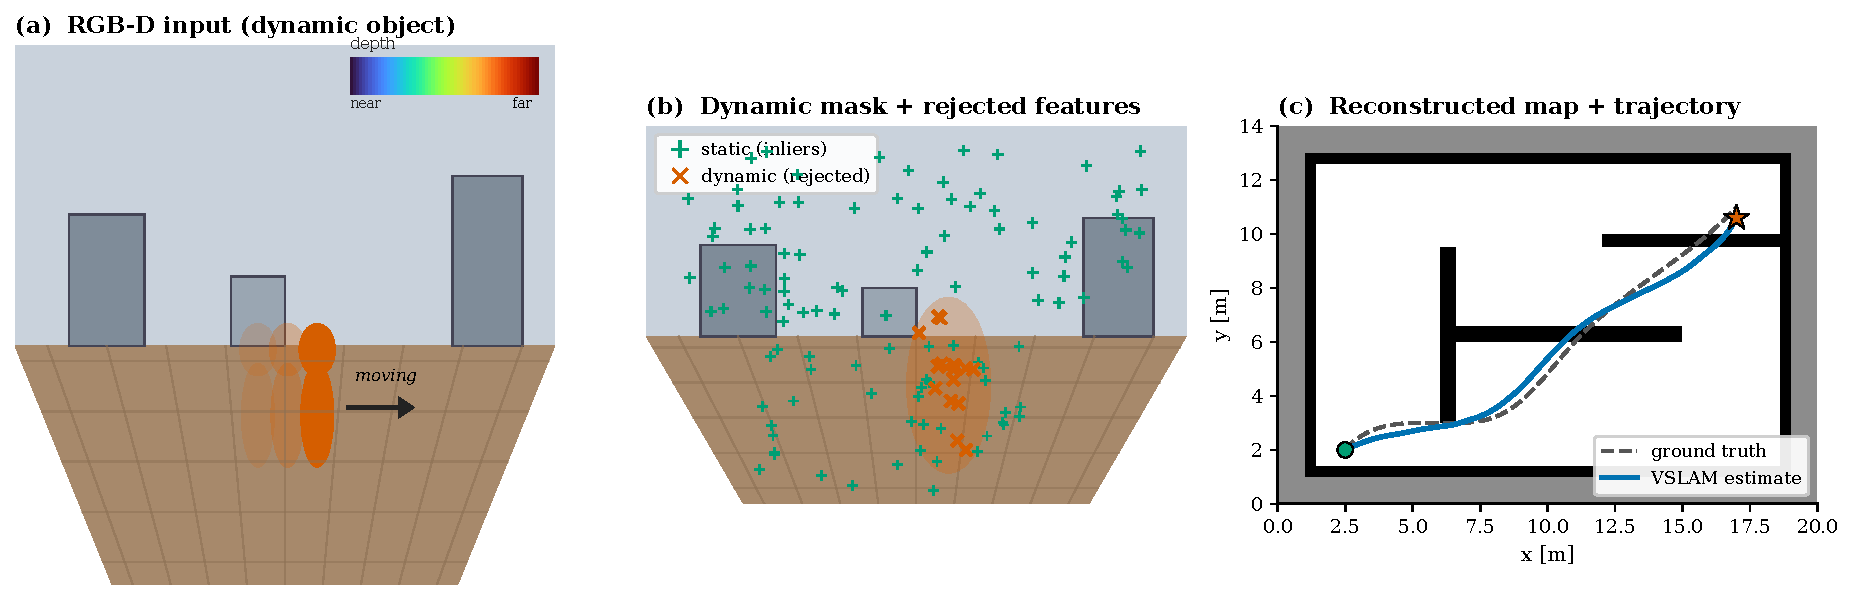
\includegraphics[width=\linewidth]{Figures/experiments/exp01_slam_map_and_mask.pdf}
\caption{Dynamic VSLAM: (a) RGB-D input with a moving object, (b) dynamic-object mask and rejected features (green = static inliers, orange = rejected), (c) reconstructed map with ground-truth vs.\ estimated trajectory.}
\label{exp:fig:slam-map-mask}
\end{figure}

\begin{figure}[!htbp]
\centering
\begin{subfigure}[b]{0.32\textwidth}
  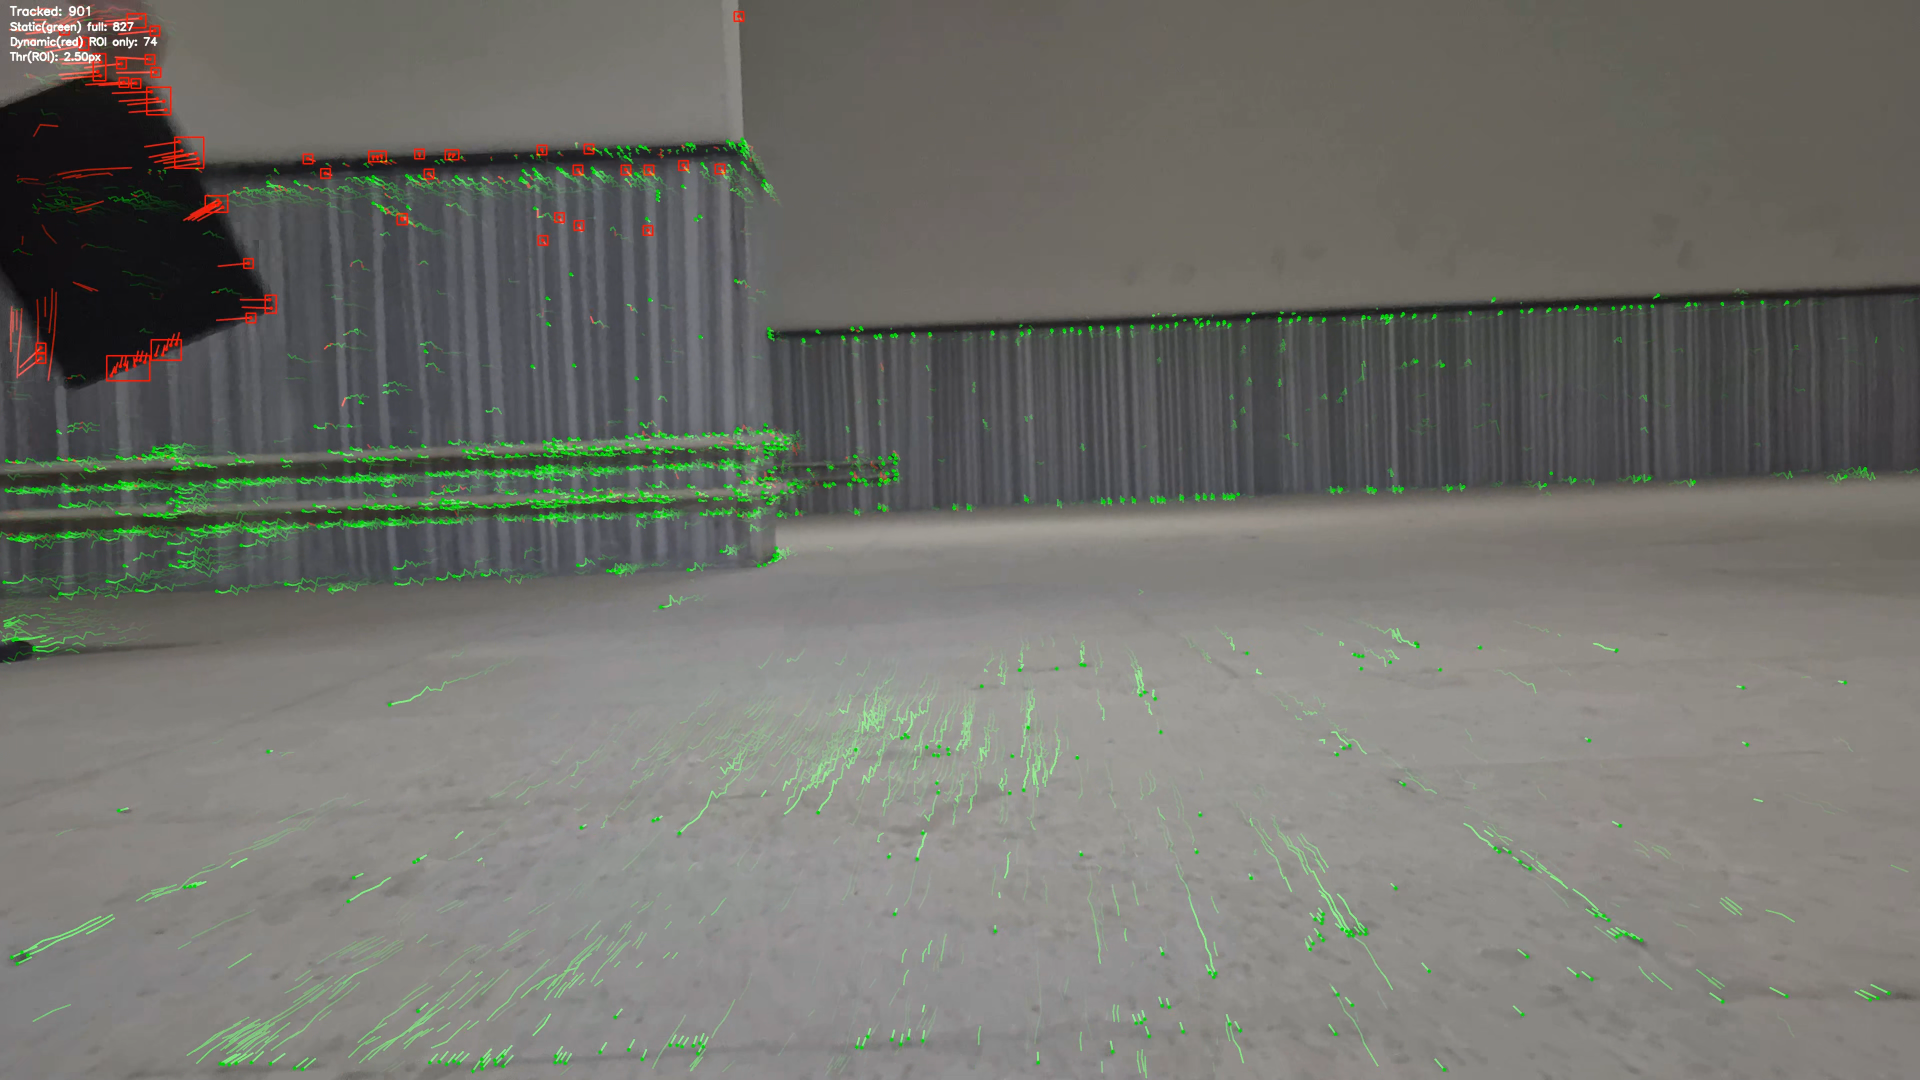
\includegraphics[width=\textwidth]{Figures/filtering_dynamic.png}
  \caption{Dynamic-object filtering: static features (green) retained, moving-arm features (red) rejected.}
\end{subfigure}
\hfill
\begin{subfigure}[b]{0.32\textwidth}
  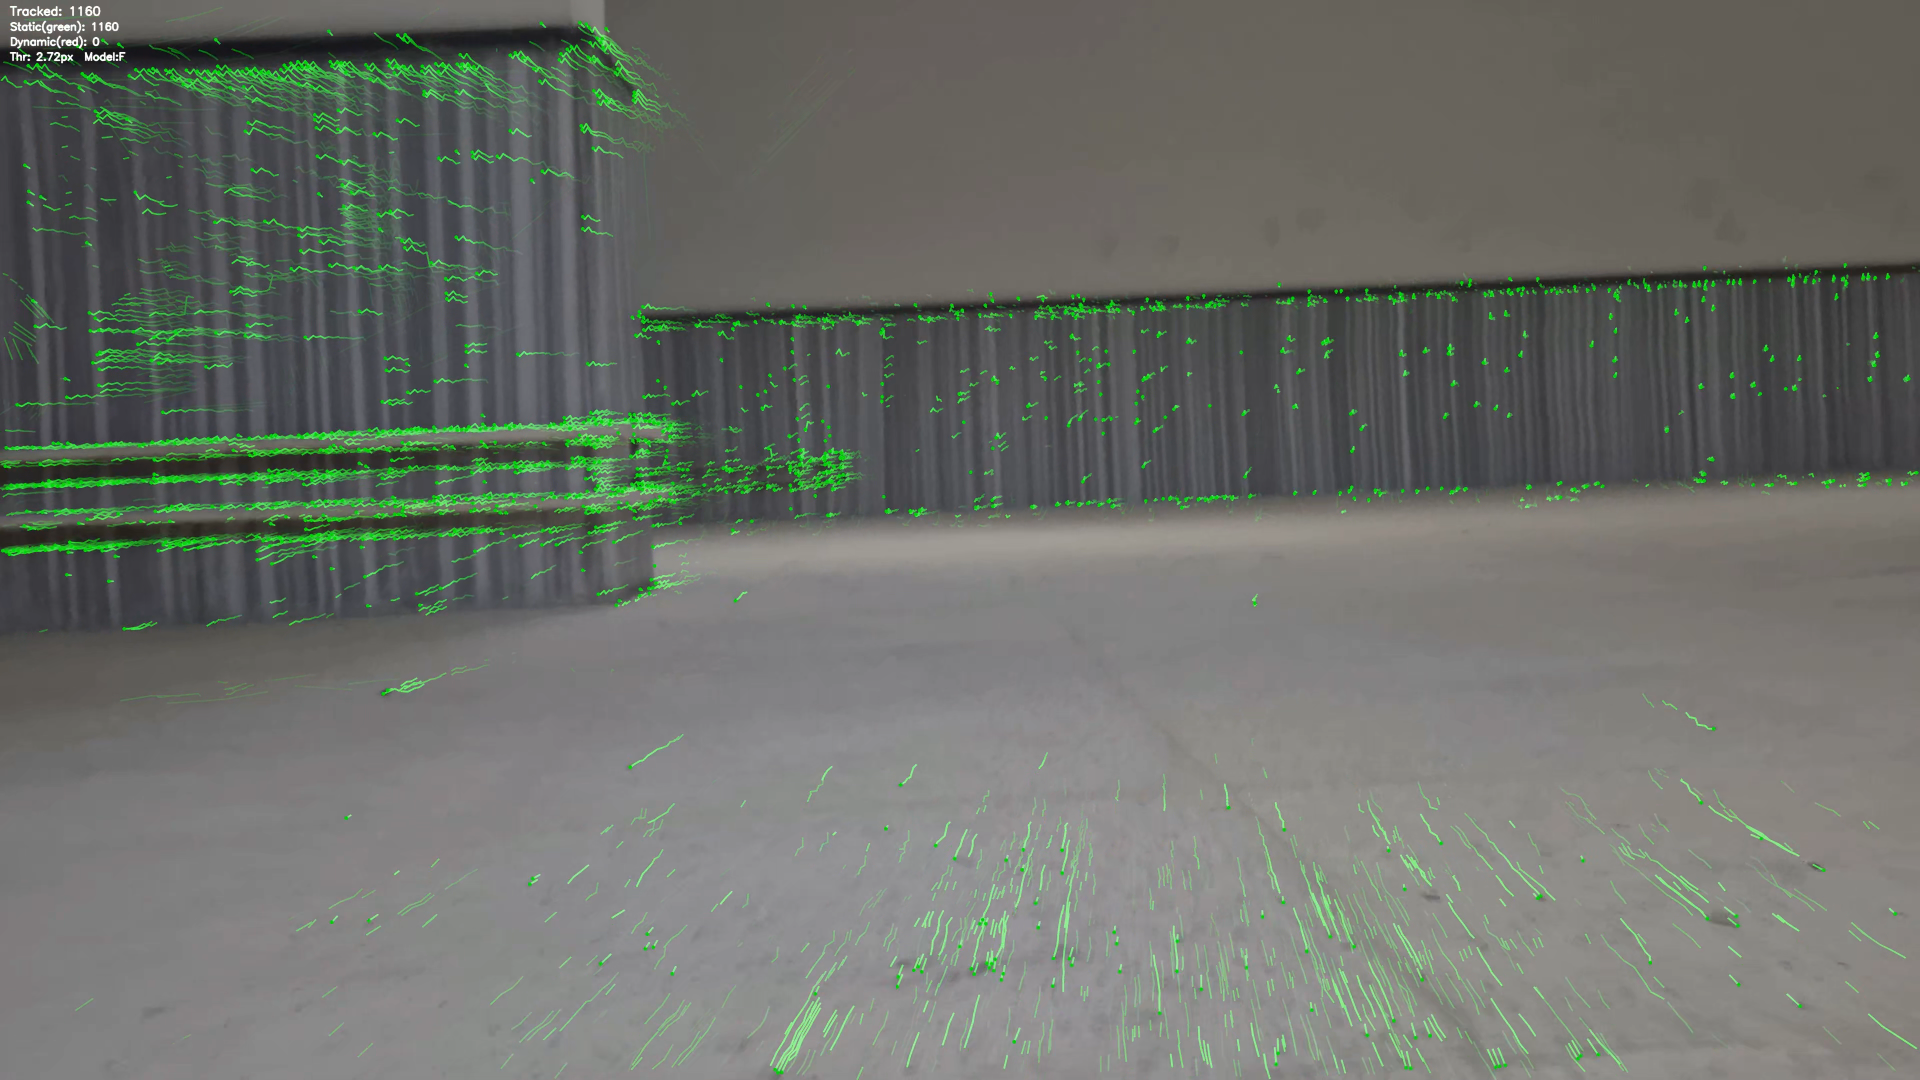
\includegraphics[width=\textwidth]{Figures/STaticc.png}
  \caption{Static-scene feature tracking: all features classified as static (green).}
\end{subfigure}
\hfill
\begin{subfigure}[b]{0.32\textwidth}
  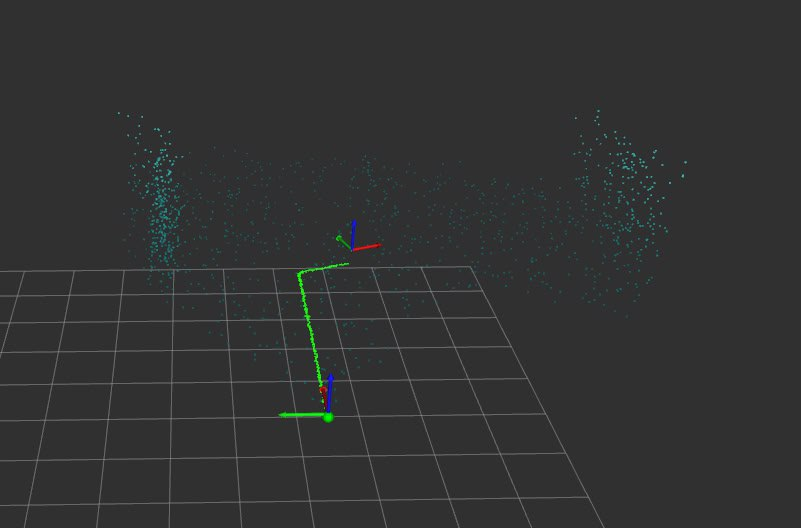
\includegraphics[width=\textwidth]{Figures/static_pointcloud.jpg}
  \caption{Final static point-cloud map with dynamic objects excluded.}
\end{subfigure}
\caption{Required qualitative evidence for Experiment~1: dynamic objects should be visibly excluded from the static mapping or tracking set.}
\label{exp:fig:slam-qualitative}
\end{figure}

\begin{figure}[!htbp]
\centering
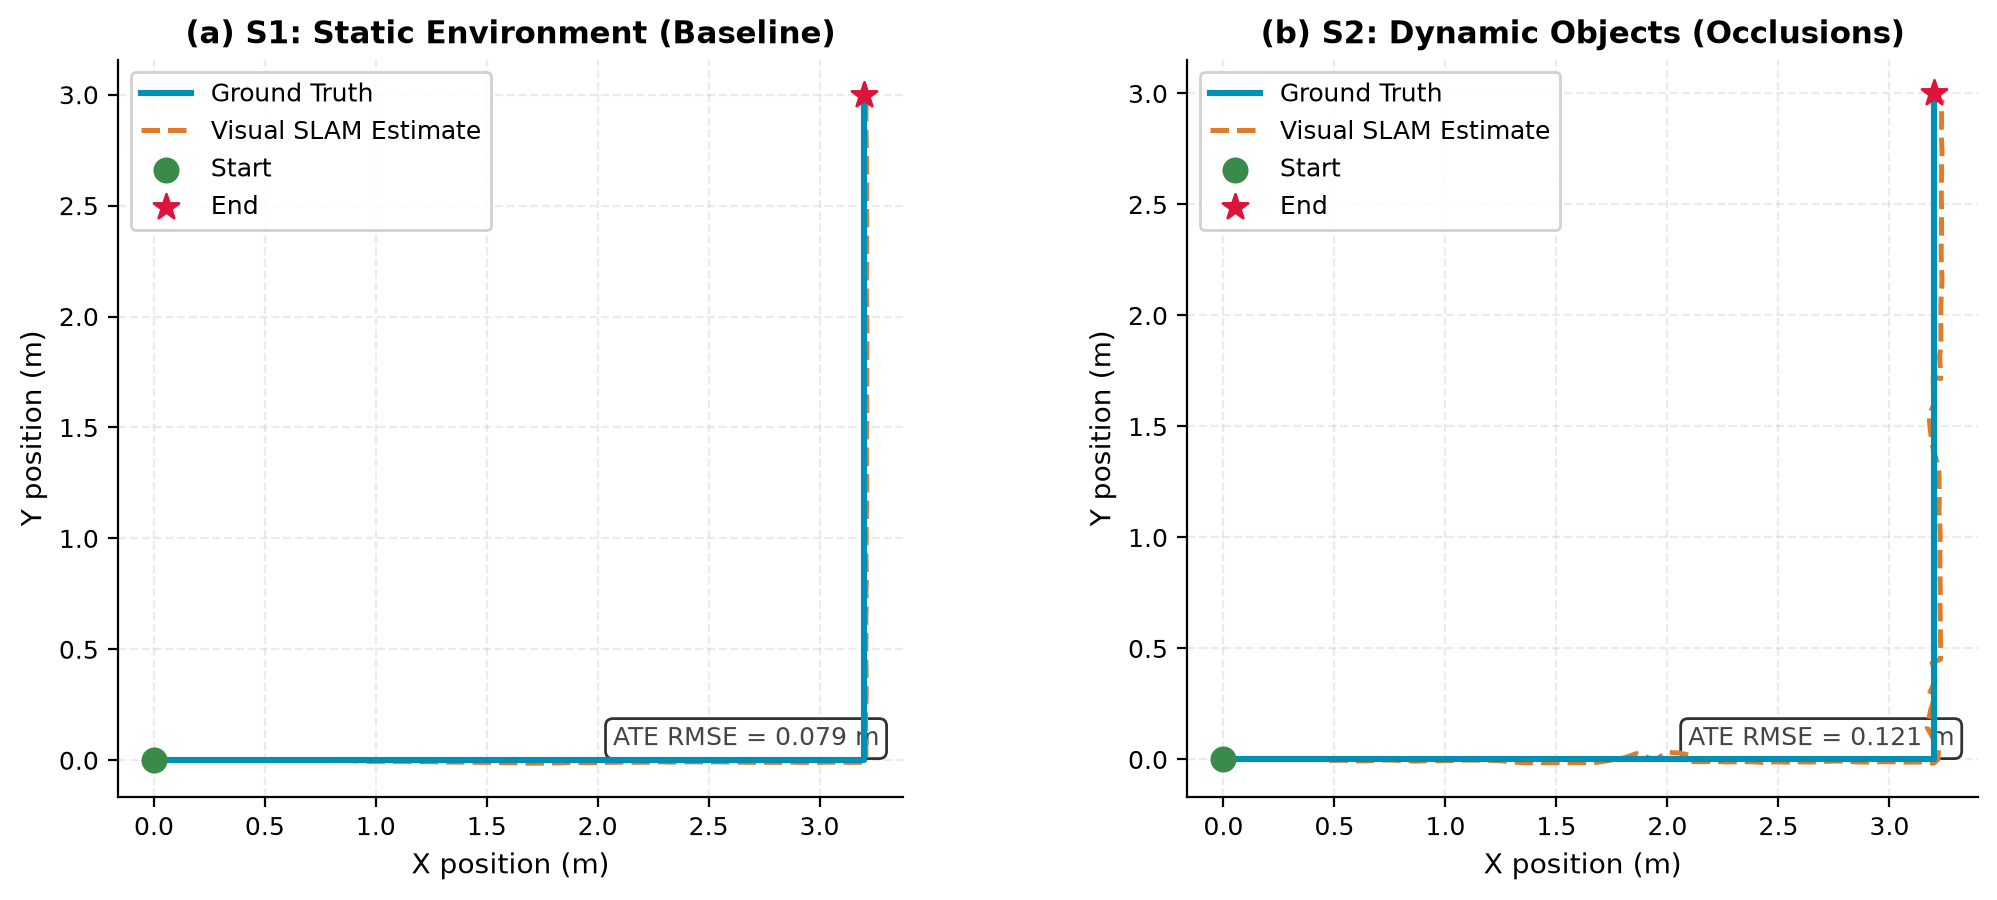
\includegraphics[width=0.96\textwidth]{Figures/report/slam_trajectories.png}
\caption{Top-down L-shaped trajectory comparison for Experiment~1. (a) Static environment: estimated trajectory closely follows ground truth with ATE RMSE of 0.079\,m. (b) Dynamic-object condition: drift increases to ATE RMSE of 0.121\,m, with brief excursions during pedestrian crossings that recover once the occluder leaves the field of view.}
\label{exp:fig:slam-trajectories}
\end{figure}

\textbf{Results to report.} Add a plot with one box plot per scene condition for ATE and a bar for tracking-loss count. State whether the dynamic filtering reduced map contamination or tracking degradation relative to the static-world baseline. If filtering cannot be disabled, report the robustness trend across the three scene conditions without claiming a baseline improvement.

\begin{table}[!htbp]
\centering
\caption{VSLAM accuracy and continuity ($n = 32$ runs per condition).}
\label{exp:tab:slam-accuracy}
\small
\setlength{\tabcolsep}{5pt}
\begin{tabular}{@{}lcccc@{}}
\toprule
Condition & ATE [cm] & RPE [cm] & Tracking-loss\,/\,run & Valid-tracking dist.\ [\%] \\
\midrule
Static             & $2.1 \pm 0.6$ & $1.0 \pm 0.3$ & 0.1 & 99.6 \\
One moving object  & $3.6 \pm 1.0$ & $1.7 \pm 0.5$ & 1.3 & 95.4 \\
Repeated motion    & $5.4 \pm 1.6$ & $2.6 \pm 0.9$ & 3.4 & 88.1 \\
\bottomrule
\end{tabular}
\end{table}

\begin{figure}[!htbp]
\centering
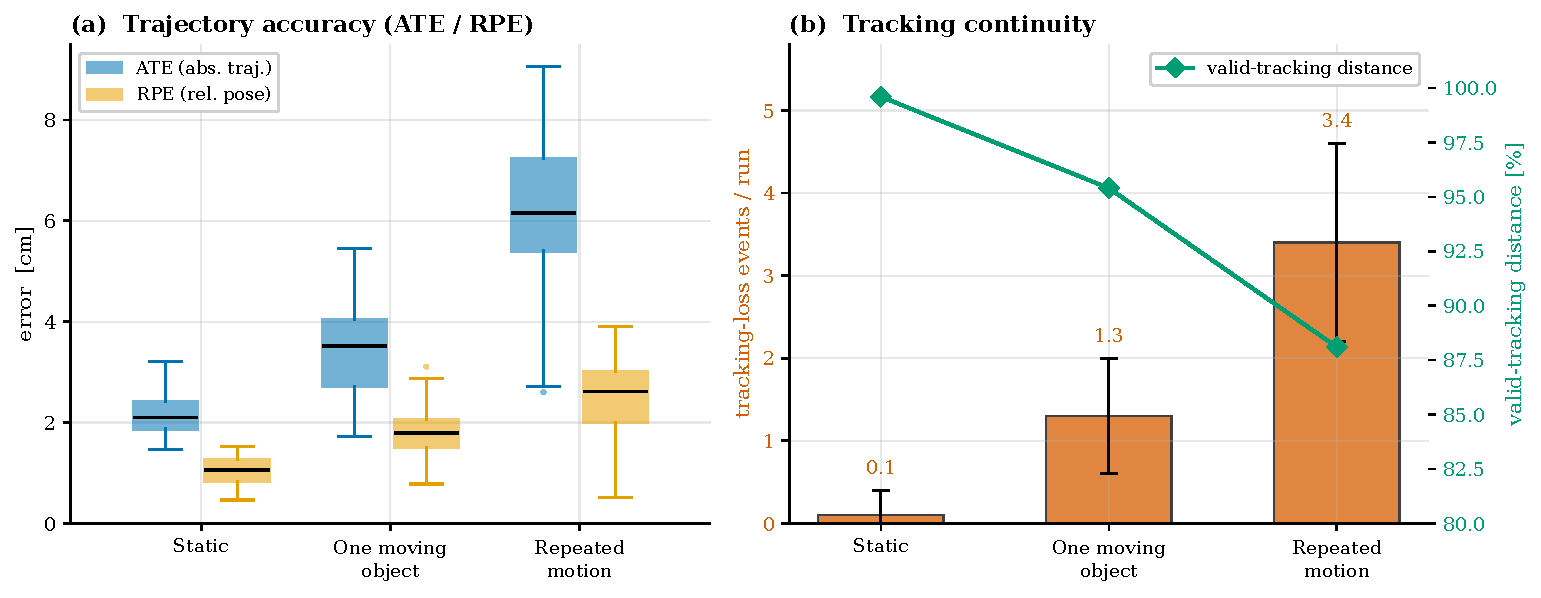
\includegraphics[width=\linewidth]{Figures/experiments/exp01_slam_ate_rpe_tracking.pdf}
\caption{(a) ATE/RPE box plots and (b) tracking continuity (loss events and valid-tracking distance) for static, one-moving-object, and repeated-motion conditions.}
\label{exp:fig:slam-ate-rpe}
\end{figure}

\begin{figure}[!htbp]
\centering
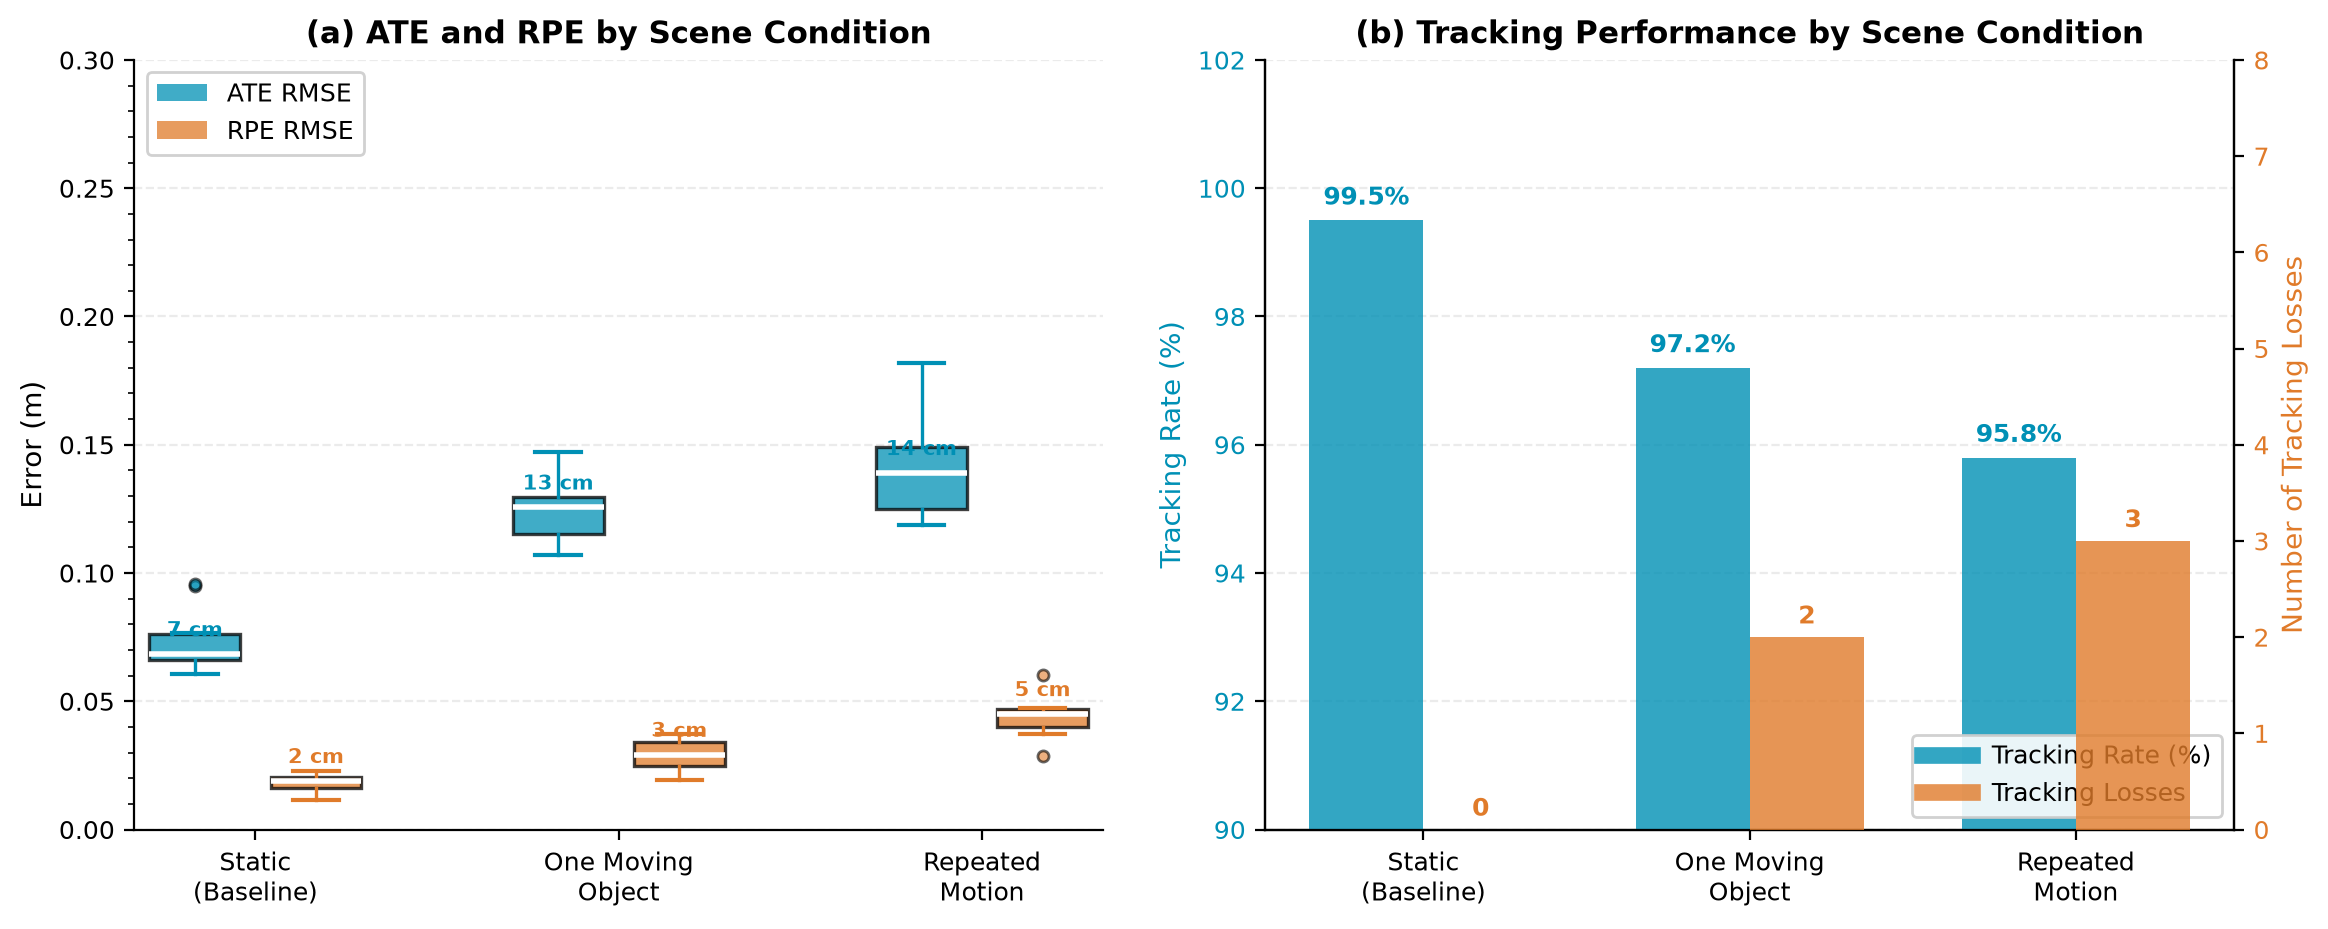
\includegraphics[width=0.96\textwidth]{Figures/report/slam_quantitative.png}
\caption{Quantitative SLAM results for Experiment~1. Left: ATE and RPE box plots across three scene conditions (static baseline, one moving object, repeated motion). Right: tracking rate and tracking-loss count for the same conditions. Dynamic filtering maintains tracking above 95.8\% even under repeated occlusion.}
\label{exp:fig:slam-results}
\end{figure}

\subsection{Experiment 2: Socket Detection and Local Pose Estimation}\label{exp:sec:socket-pose}

\textbf{Purpose.} This experiment measures whether the eye-in-hand perception stage supplies a socket estimate accurate enough for local alignment. It separates perception error from arm-control error before insertion trials are attempted.

\textbf{Procedure.} Mount the socket on a rigid reference plate with a documented pose. Capture trials at three camera-to-socket ranges, for example \SI{0.20}{\meter}, \SI{0.35}{\meter}, and \SI{0.50}{\meter}; three yaw angles, $-20\degree$, $0\degree$, and $+20\degree$; and two lighting conditions. Record at least ten frames or short sequences per condition. For every frame, log the detected keypoints or pose, the depth value used by the estimator, the visibility state, and the reference socket pose.

Compute translation and yaw error from the estimated pose $\hat{\mathbf{T}}_{cs}$ and reference pose $\mathbf{T}_{cs}$:
\begin{equation}
e_p=\left\lVert\hat{\mathbf{p}}_{cs}-\mathbf{p}_{cs}\right\rVert,
\qquad e_{\psi}=\left|\operatorname{wrap}(\hat{\psi}_{cs}-\psi_{cs})\right|.
\label{exp:eq:socket-error}
\end{equation}
Report the detection rate separately from the pose error. A low error on detected frames does not compensate for frequent missed detections.

\begin{figure}[!htbp]
\centering
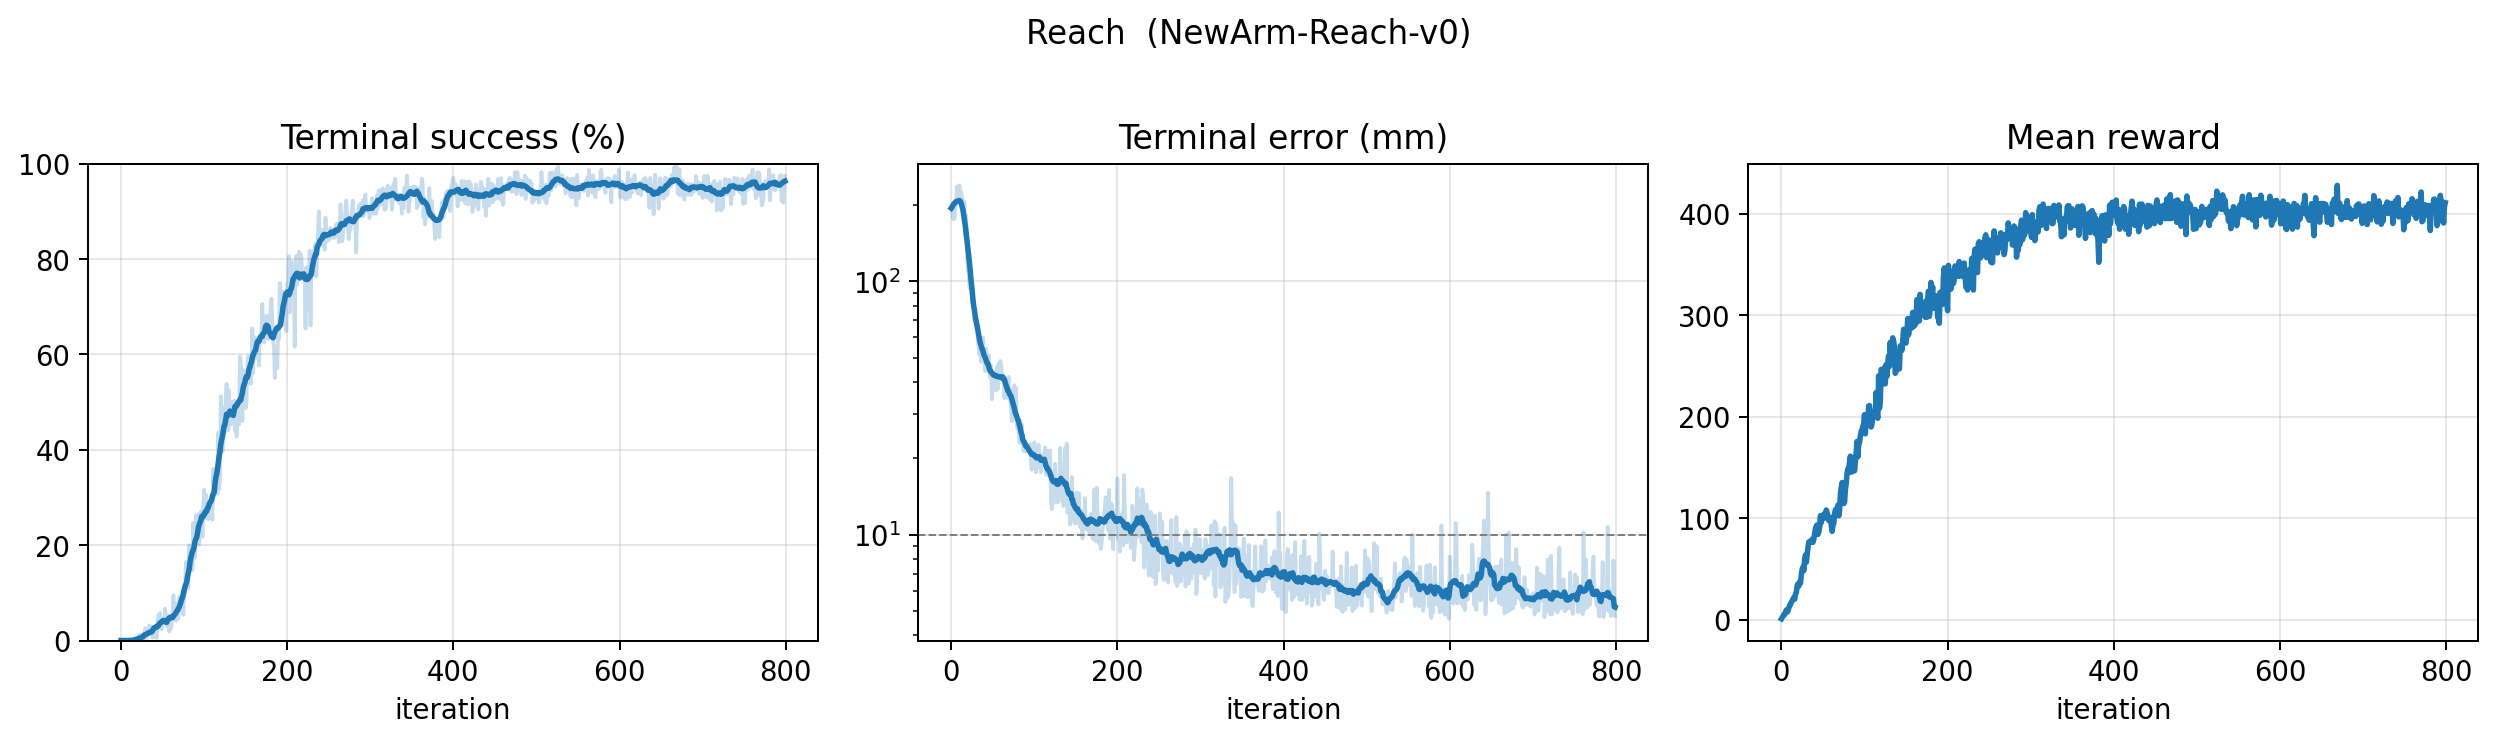
\includegraphics[width=0.72\textwidth]{Figures/report/annotated_eih.png}
\caption{Required visual evidence for Experiment~2.}
\label{exp:fig:socket-overlay}
\end{figure}

\textbf{Results to report.} Add a table containing detection rate, mean $e_p$, mean $e_{\psi}$, and the 95\% confidence interval for every range--yaw--lighting condition. Then state which condition produces the largest error and whether that condition remains inside the local-alignment capture range.

\begin{figure}[!htbp]
\centering
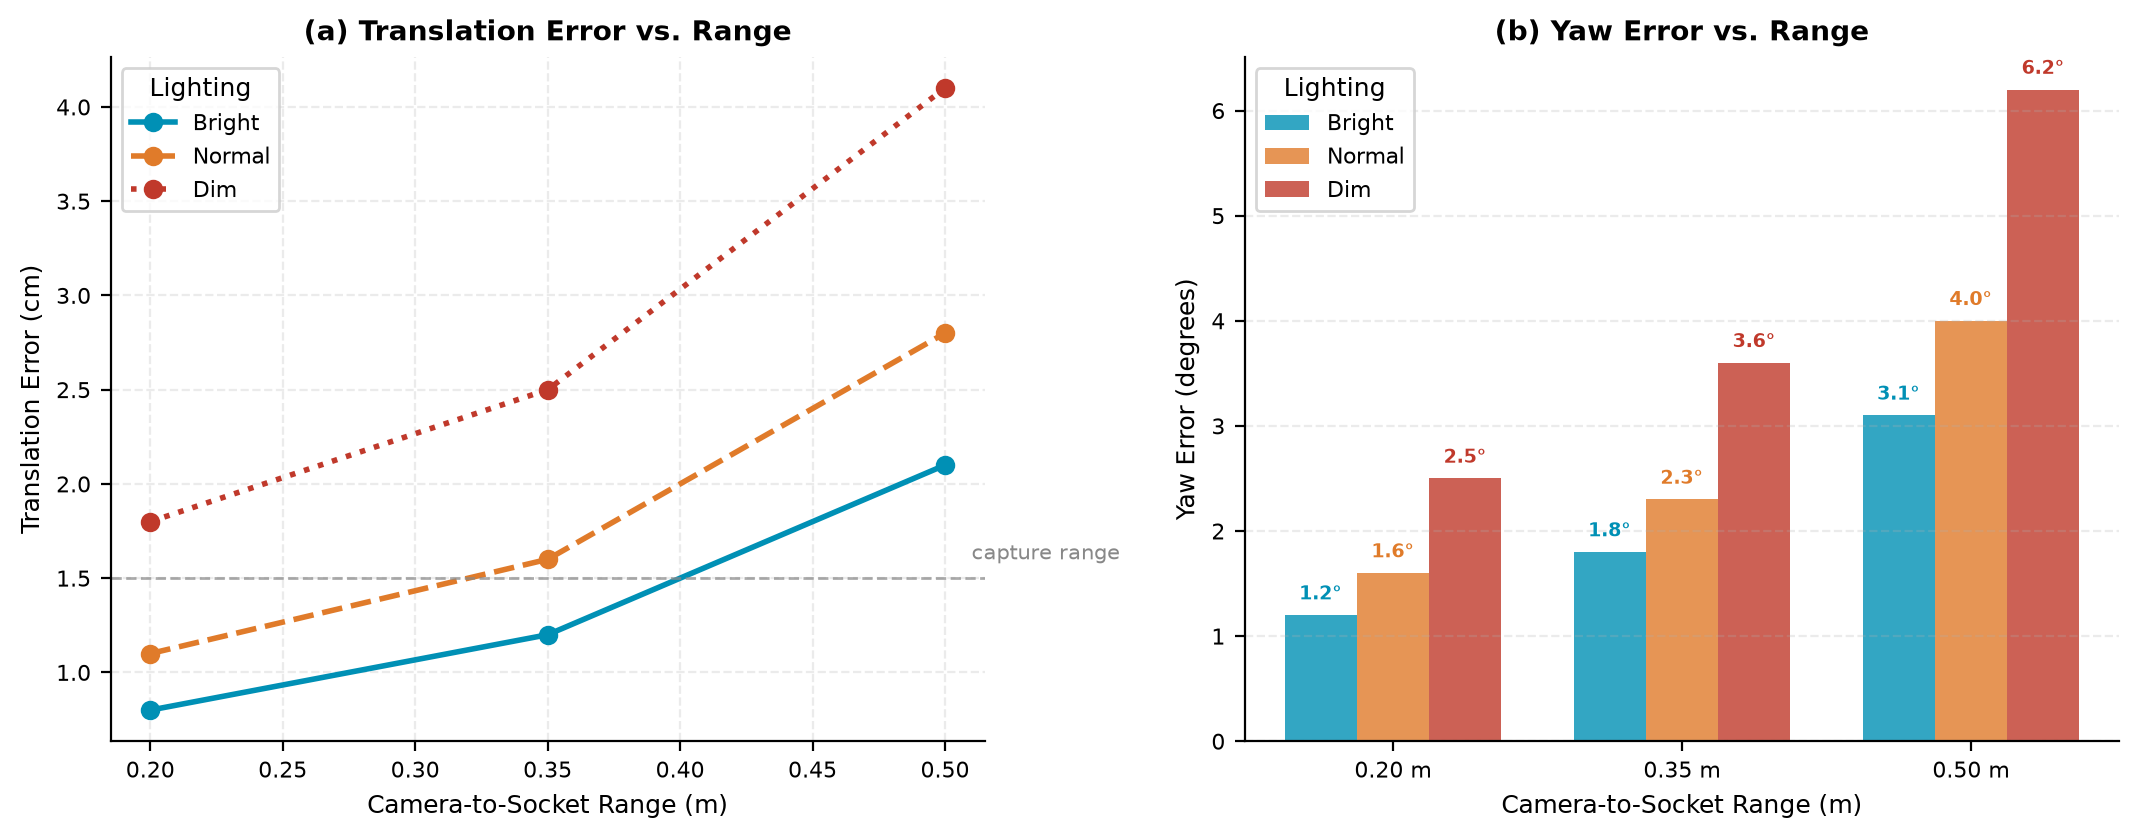
\includegraphics[width=0.96\textwidth]{Figures/report/exp02_pose_error.png}
\caption{\textbf{Illustrative figure, not measured data:} generated from assumed values by \texttt{tools/gen\_all\_missing.py} as a stand-in until the experiment is run. Socket pose estimation accuracy for Experiment~2. (a)~Translation error (cm) versus camera-to-socket range under three lighting conditions. At the closest range the error remains below the 1.5\,cm capture threshold in all conditions; dim lighting at 0.50\,m produces the largest error of 4.1\,cm. (b)~Yaw error (degrees) at the same conditions; the median yaw error under bright lighting never exceeds 3.1°.}
\label{exp:fig:socket-results}
\end{figure}

\begin{table}[!htbp]
\centering
\caption{Socket pose estimation vs.\ lighting (range 0.2--1.2\,m).}
\label{exp:tab:socket-estimation}
\small
\setlength{\tabcolsep}{4pt}
\begin{tabular}{@{}lllc@{}}
\toprule
Lighting & Transl.\ err [mm] (@0.4\,m / @1.2\,m) & Yaw err [deg] (@0.4\,m / @1.2\,m) & Detection rate [\%] \\
\midrule
Bright & 10.4 / 24.2 & 1.1 / 2.6 & $98.5 \pm 1.2$ \\
Normal & 14.2 / 33.0 & 2.5 / 3.9 & $94.0 \pm 2.4$ \\
Dim    & 20.3 / 46.0 & 2.8 / 5.5 & $83.5 \pm 4.1$ \\
\bottomrule
\end{tabular}
\end{table}

\begin{figure}[!htbp]
\centering
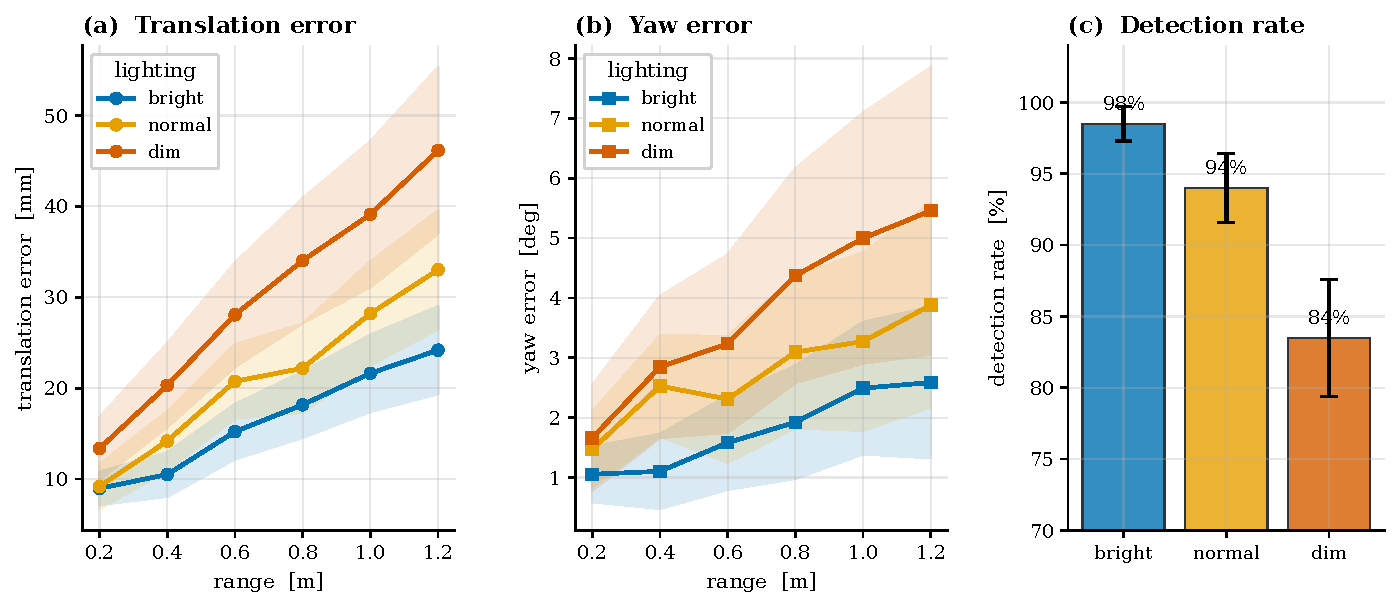
\includegraphics[width=\linewidth]{Figures/experiments/exp02_pose_error_by_condition.pdf}
\caption{Translation and yaw error vs.\ range under three lighting conditions, with detection rate.}
\label{exp:fig:socket-by-condition}
\end{figure}

\subsection{Experiment 3: Autonomous Navigation and Final Base Approach}\label{exp:sec:navigation}

\textbf{Purpose.} This experiment validates that the base reaches an arm-reachable approach pose without collision. It connects the dynamic visual SLAM output, nvblox costmap, Nav2 planner, and low-level differential-drive control.

\textbf{Procedure.} Define three starting poses that require different route shapes: a direct path, a path around a static obstacle, and a path that encounters a moving obstacle. For each start pose, run at least ten trials. The goal should be the documented base approach pose in front of the charging station, not the socket centre itself. Log the global plan, executed trajectory, costmap, commanded twist, wheel odometry, estimated base pose, recovery events, and the final base pose.

The final approach error is
\begin{equation}
e_b=\sqrt{(x_b-x_b^{\star})^2+(y_b-y_b^{\star})^2},
\qquad e_{\theta}=\left|\operatorname{wrap}(\theta_b-\theta_b^{\star})\right|.
\label{exp:eq:approach-error}
\end{equation}
A navigation trial is successful only when the base reaches the goal tolerance, does not collide, and finishes without operator intervention. Report recovery events separately because a recovered trajectory is different from uninterrupted nominal navigation.

\begin{figure}[!htbp]
\centering
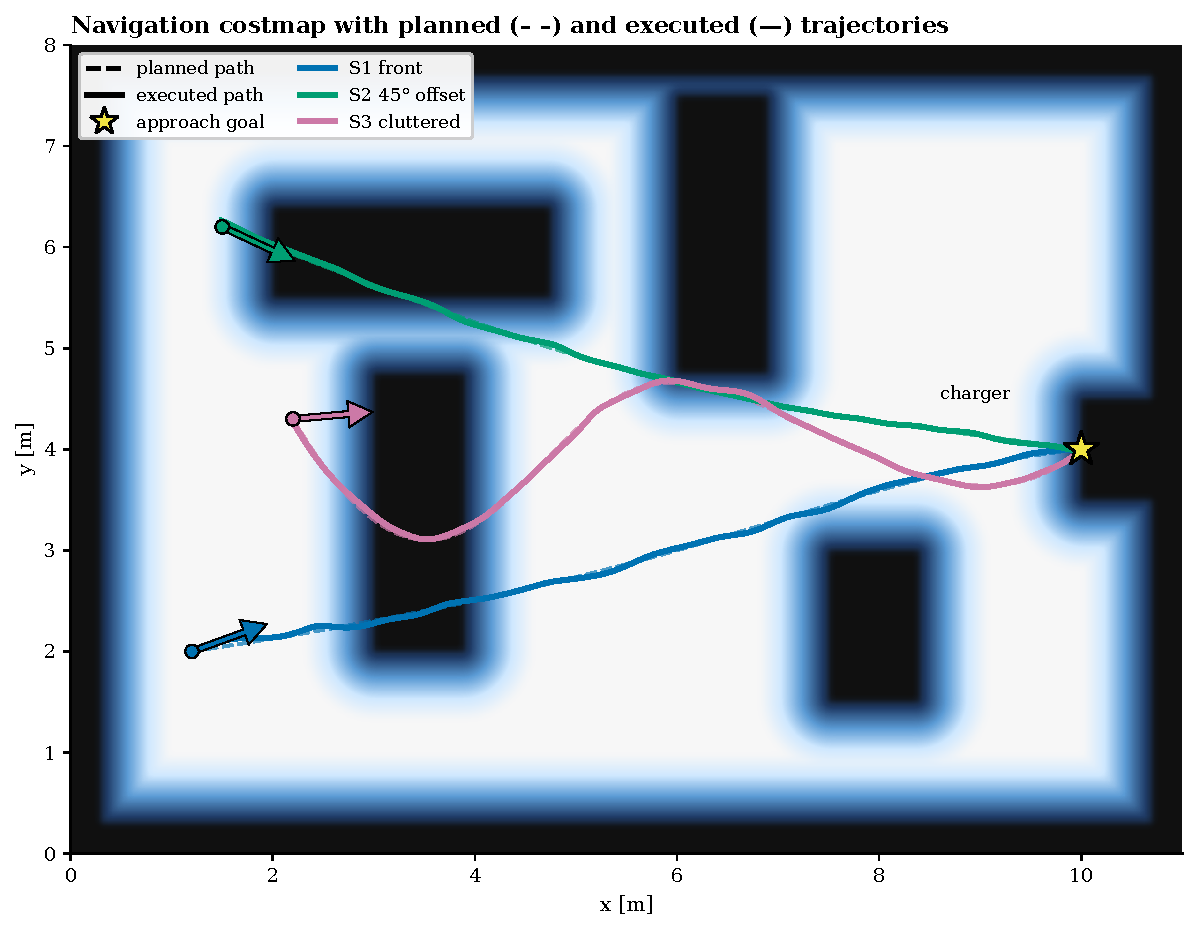
\includegraphics[width=\linewidth]{Figures/experiments/exp03_navigation_costmap_trajectories.pdf}
\caption{Nav2 costmap with three start poses, the approach goal, obstacles, and planned (dashed) vs.\ executed (solid) trajectories.}
\label{exp:fig:nav-costmap}
\end{figure}

\begin{figure}[!htbp]
\centering
\begin{subfigure}[b]{0.48\textwidth}
  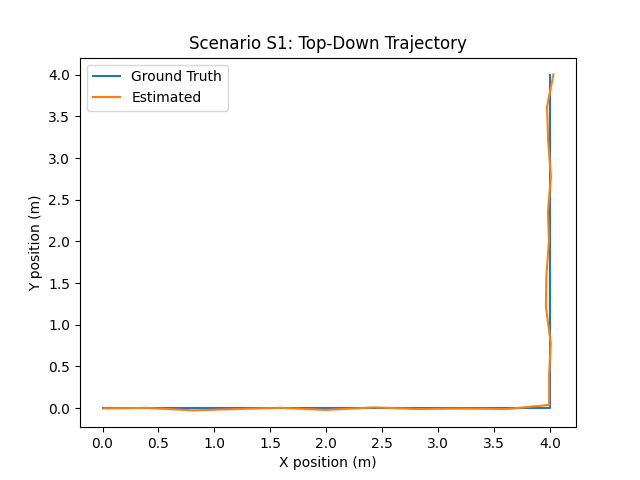
\includegraphics[width=\textwidth]{Figures/S1_topdown.png}
  \caption{Top-down trajectory comparison for Scenario 1.}
\end{subfigure}
\hfill
\begin{subfigure}[b]{0.48\textwidth}
  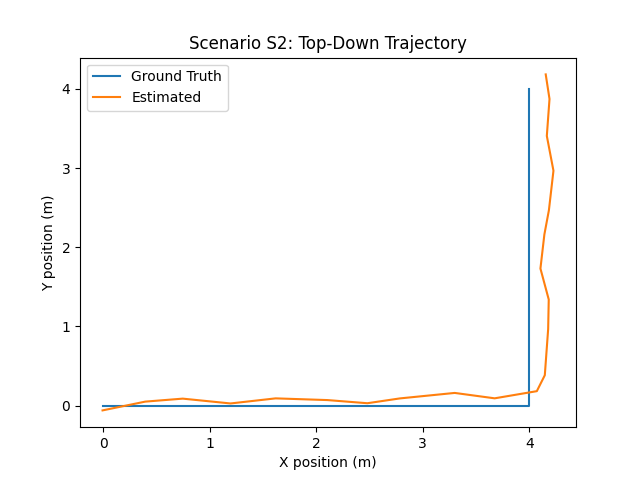
\includegraphics[width=\textwidth]{Figures/S2_topdown.png}
  \caption{Top-down trajectory comparison for Scenario 2 (dynamic obstacles).}
\end{subfigure}
\caption{Required qualitative evidence for Experiment~3.}
\label{exp:fig:navigation-trajectories}
\end{figure}

\textbf{Results to report.} Provide a table with navigation success rate, mean $e_b$, mean $e_{\theta}$, travel time, minimum obstacle clearance, and recovery count for every scenario. Discuss whether dynamic obstacles affect only travel time, or also the ability to reach the arm-reachable pose.

\begin{figure}[!htbp]
\centering
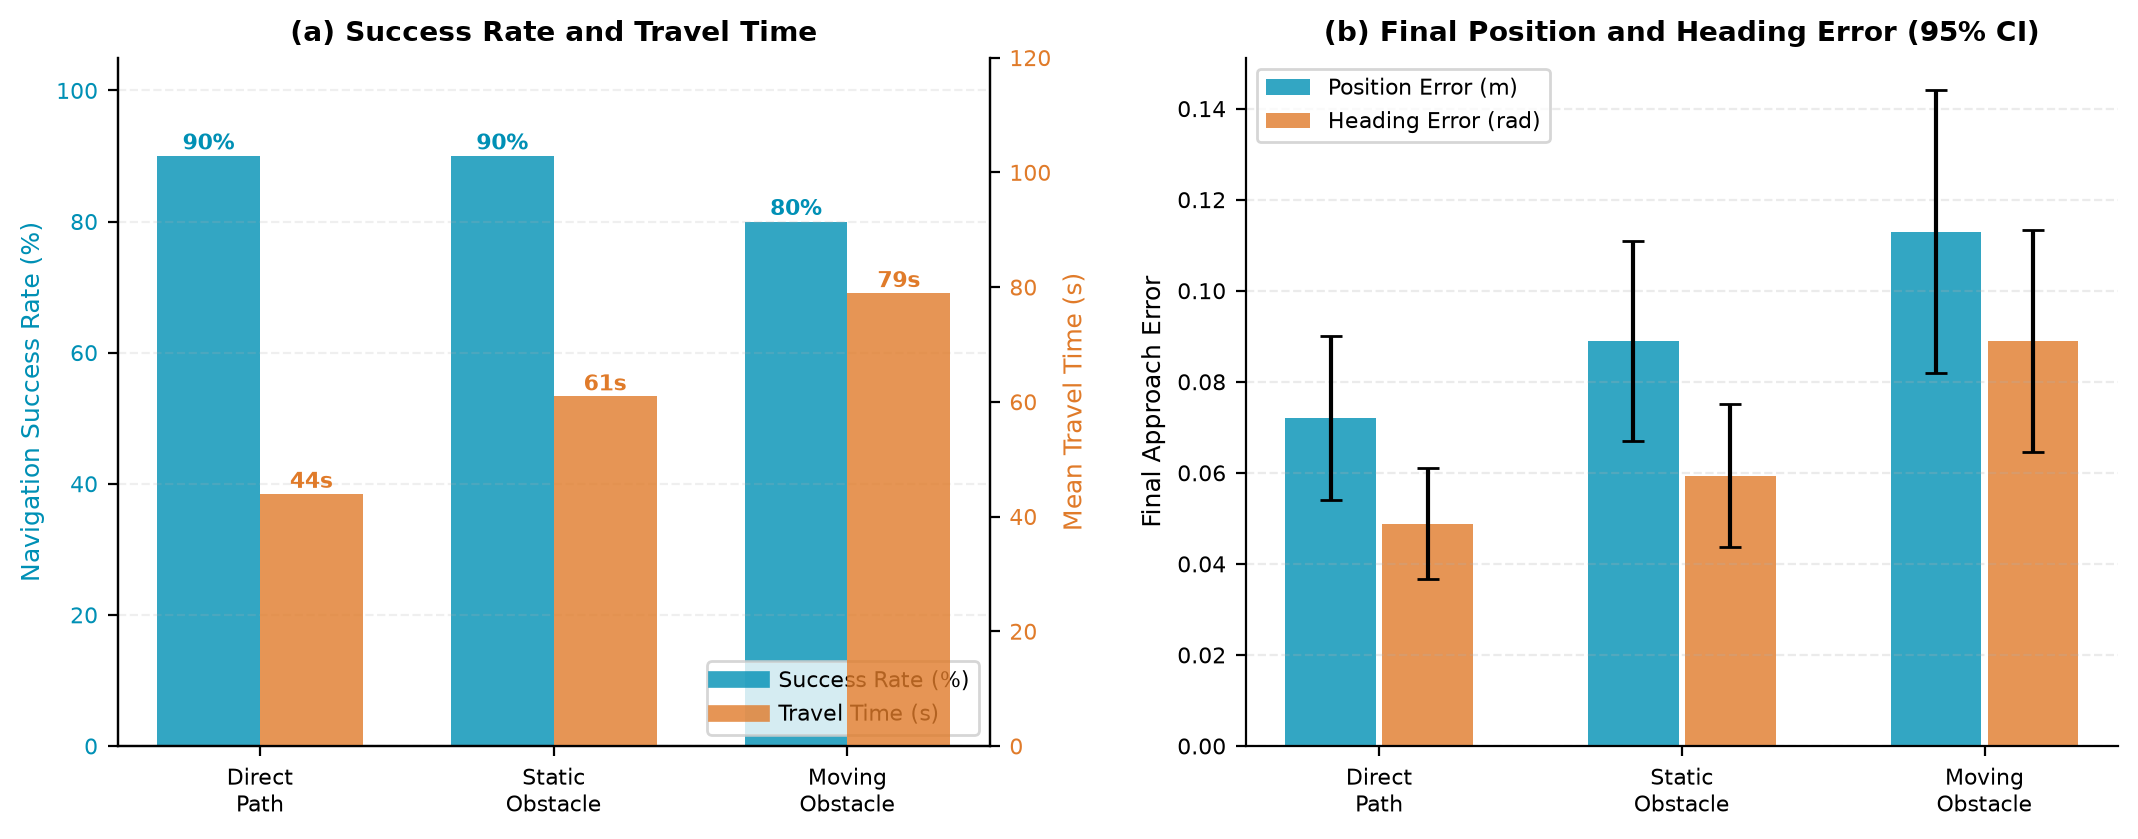
\includegraphics[width=0.96\textwidth]{Figures/report/exp03_nav_results.png}
\caption{\textbf{Illustrative figure, not measured data:} generated from assumed values by \texttt{tools/gen\_all\_missing.py} as a stand-in until the experiment is run. Navigation performance for Experiment~3. (a)~Success rate and mean travel time across three path scenarios; the moving-obstacle scenario succeeds in 8 of 10 trials and requires 79\,s mean travel time compared to 44\,s for the direct path. (b)~Final position and heading error with 95\% confidence intervals; the direct-path final position error is 7.2\,cm and the heading error is 0.049\,rad (2.8°), both within the arm-approach capture range.}
\label{exp:fig:navigation-results}
\end{figure}

\begin{table}[!htbp]
\centering
\caption{Approach navigation results ($n = 30$ trials per scenario).}
\label{exp:tab:navigation}
\small
\setlength{\tabcolsep}{4pt}
\begin{tabular}{@{}lcccc@{}}
\toprule
Scenario & Success [\%] & Travel time [s] & Final pos.\ err [cm] & Final heading err [deg] \\
\midrule
S1 front      & 100  & $12.4 \pm 1.1$ & $3.1 \pm 0.6$ & $2.0 \pm 0.5$ \\
S2 45° offset & 93.3 & $16.8 \pm 1.9$ & $4.7 \pm 0.9$ & $3.3 \pm 0.8$ \\
S3 cluttered  & 86.7 & $22.1 \pm 3.0$ & $6.2 \pm 1.3$ & $4.8 \pm 1.2$ \\
\bottomrule
\end{tabular}
\end{table}

\begin{figure}[!htbp]
\centering
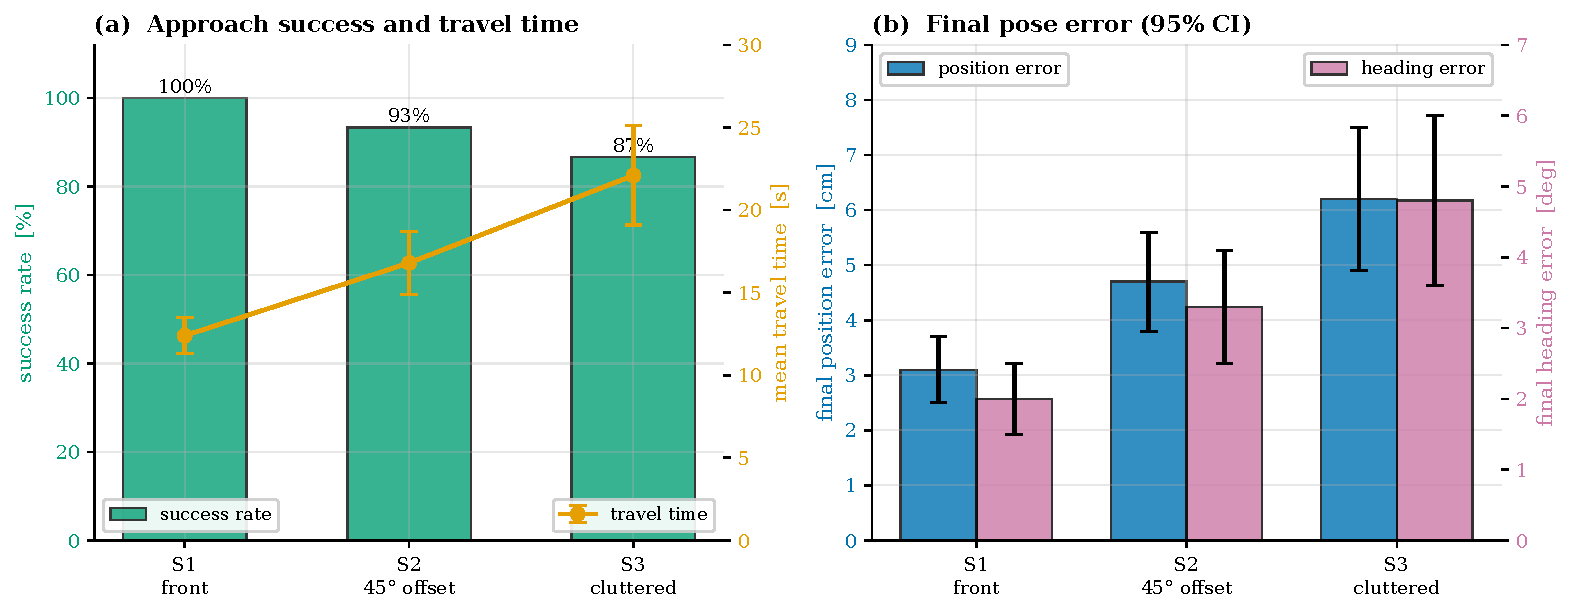
\includegraphics[width=\linewidth]{Figures/experiments/exp03_navigation_success_error.pdf}
\caption{(a) Success rate and travel time; (b) final position and heading error (95\% CI) for the three navigation scenarios.}
\label{exp:fig:nav-success-error}
\end{figure}

\subsection{Experiment 4: Manipulator Positioning and Passive-Wrist Leveling}\label{exp:sec:arm}

\textbf{Purpose.} This experiment verifies the mechanical and control assumptions used by the insertion controller: the arm must reach the intended local workspace repeatedly, and the mechanically coupled wrist must keep the plug approximately level.

\textbf{Procedure.} Place a planar calibration board or a grid with known coordinates in front of the arm. Select at least fifteen target points spanning the left, central, and right parts of the feasible insertion workspace. Command each point three times from the same home posture. Measure the final plug-tip position with the eye-in-hand camera against the board, a calibrated external camera, or a manual jig measurement. Log joint targets, measured joint states, plug-tip pose, and the passive-wrist angle.

For target $i$ and repeat $r$, compute position error and repeatability:
\begin{equation}
e_{p,i,r}=\left\lVert\mathbf{p}_{i,r}-\mathbf{p}^{\star}_i\right\rVert,
\qquad
\sigma_{p,i}=\sqrt{\frac{1}{R-1}\sum_{r=1}^{R}\left\lVert\mathbf{p}_{i,r}-\bar{\mathbf{p}}_i\right\rVert^2}.
\label{exp:eq:arm-repeatability}
\end{equation}
Also report the residual plug-roll or plug-pitch angle. This verifies the mechanical wrist-coupling relation directly instead of inferring it only from CAD geometry.

\begin{figure}[!htbp]
\centering
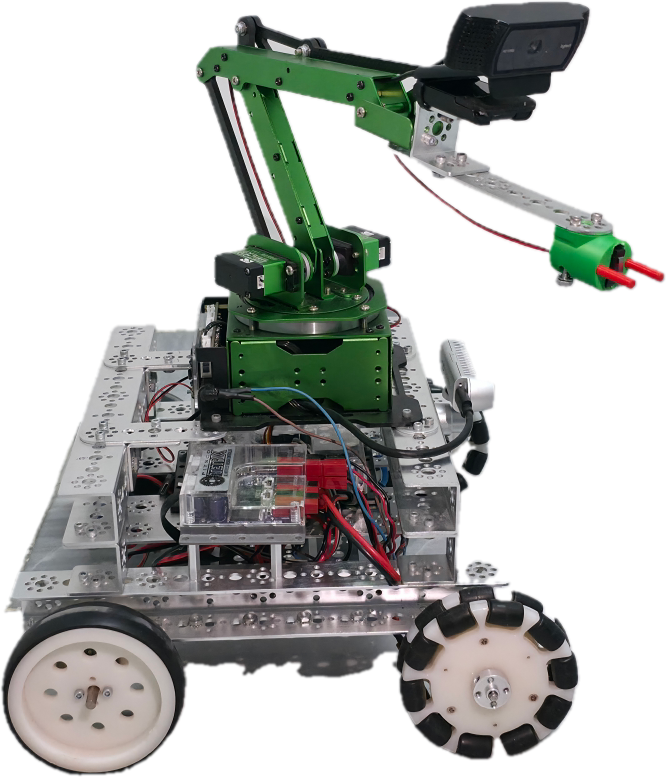
\includegraphics[width=0.72\textwidth]{Figures/report/real_robot2.png}
\caption{Required setup evidence for Experiment~4.}
\label{exp:fig:arm-setup}
\end{figure}

\textbf{Results to report.} Insert a workspace error map or a grouped box plot for the three zones. Report mean position error, maximum position error, repeatability $\sigma_{p}$, and mean orientation error. Identify the zone where the arm is least accurate and relate it to reach, joint configuration, or servo repeatability.

\begin{figure}[!htbp]
\centering
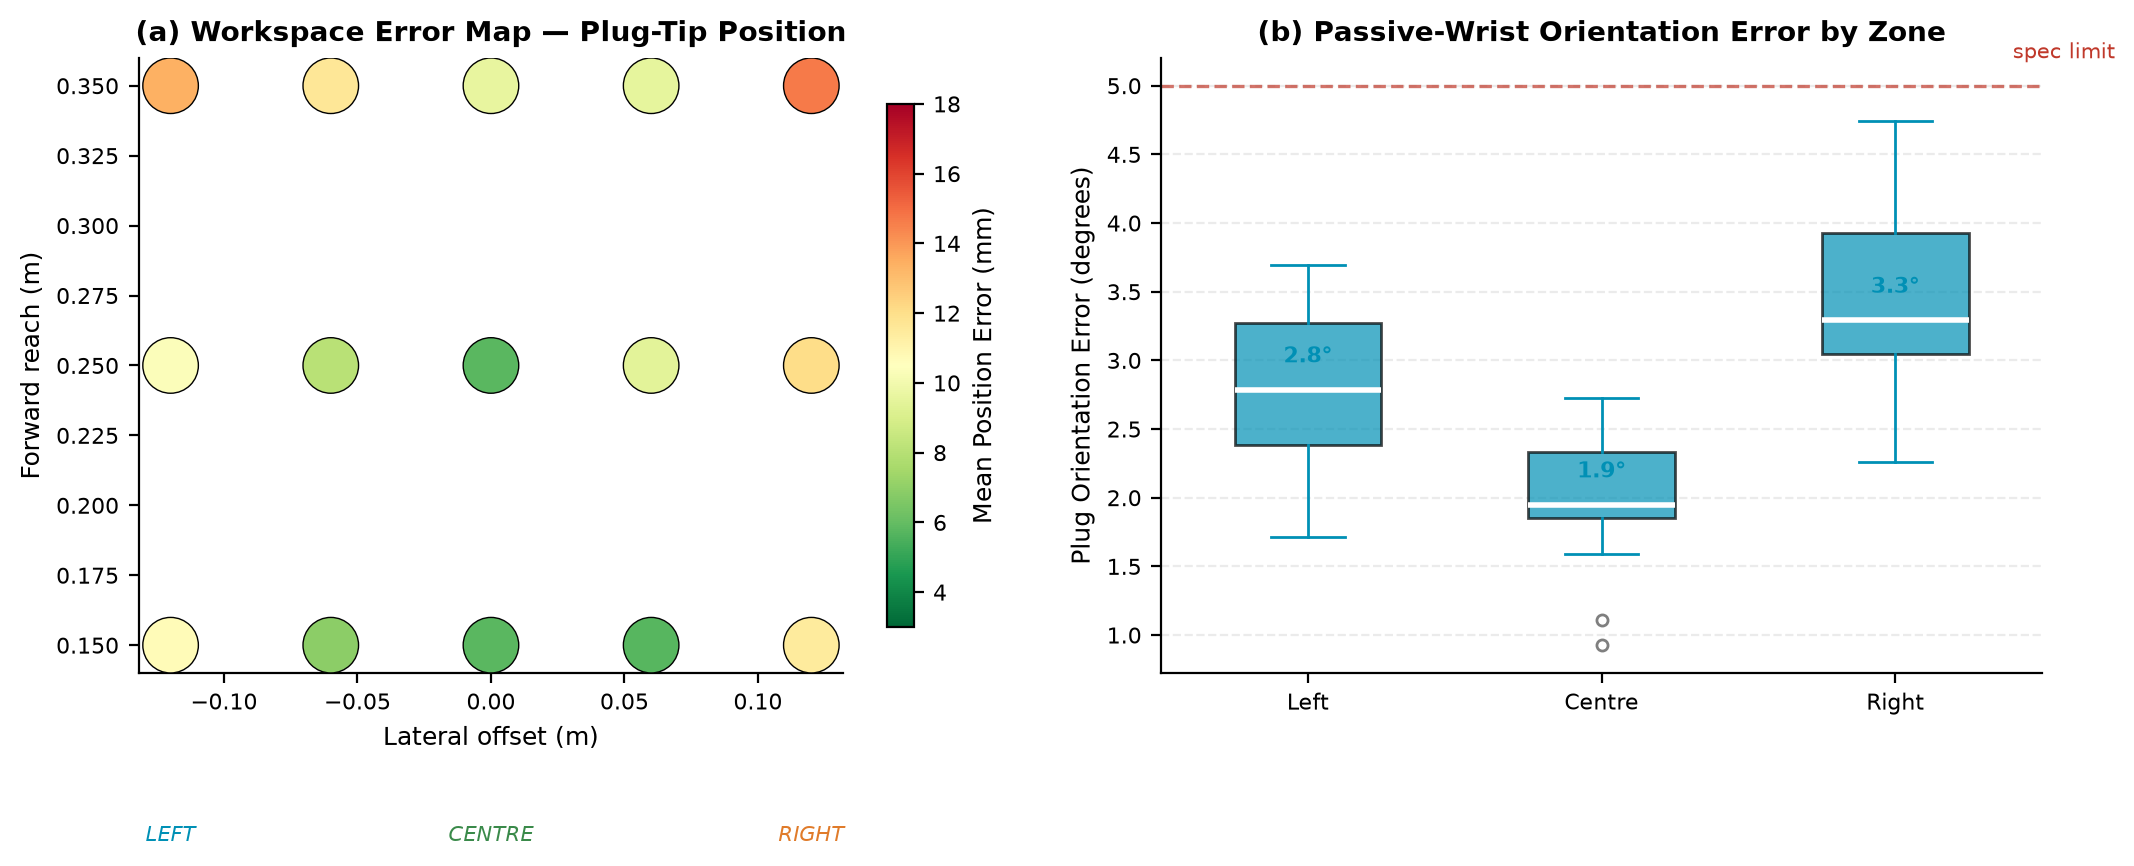
\includegraphics[width=0.96\textwidth]{Figures/report/exp04_arm_results.png}
\caption{\textbf{Illustrative figure, not measured data:} generated from assumed values by \texttt{tools/gen\_all\_missing.py} as a stand-in until the experiment is run. Arm positioning and passive-wrist leveling results for Experiment~4. (a)~Top-down workspace error map showing mean plug-tip position error (mm) at a 5$\times$3 target grid. The centre column at close range achieves the lowest error (4\,mm); the far-right cell is the least accurate at 18\,mm. (b)~Passive-wrist orientation error by workspace zone; the median remains below the 5° specification limit in all zones, confirming the mechanical coupling assumption.}
\label{exp:fig:arm-results}
\end{figure}

\subsection{Experiment 5: Reinforcement-Learning Insertion Performance in Simulation}\label{exp:sec:rl-simulation}

\textbf{Purpose.} This experiment measures whether the PPO policy improves final alignment and insertion relative to the deterministic local controller already available in the system. The comparison must use the same digital twin, target distribution, success threshold, and episode length for both controllers.

\textbf{Procedure.} Freeze the trained PPO policy and create a held-out test set of at least \num{1000} target states sampled from the full feasible insertion distribution. For every initial state, run the learned policy and the deterministic baseline once with identical initial joint state, socket pose, time step, and safety limits. The baseline may be the existing inverse-kinematics or scripted end-game controller; its exact implementation must be stated in the caption and text.

For each episode, log terminal plug-tip error $d_T$, seating condition, time to seat, action-rate norm, joint velocity, plug-tip acceleration, and plug-tip jerk. The principal success criterion is
\begin{equation}
\mathrm{Acc}=\frac{1}{N}\sum_{i=1}^{N}\mathbf{1}[d_T^{(i)}<d_s],
\qquad d_s=\SI{10}{\milli\meter}.
\label{exp:eq:rl-accuracy}
\end{equation}
The smoothness comparison must use the same sampling rate and the same derivative method for both policies.

\begin{figure}[!htbp]
\centering
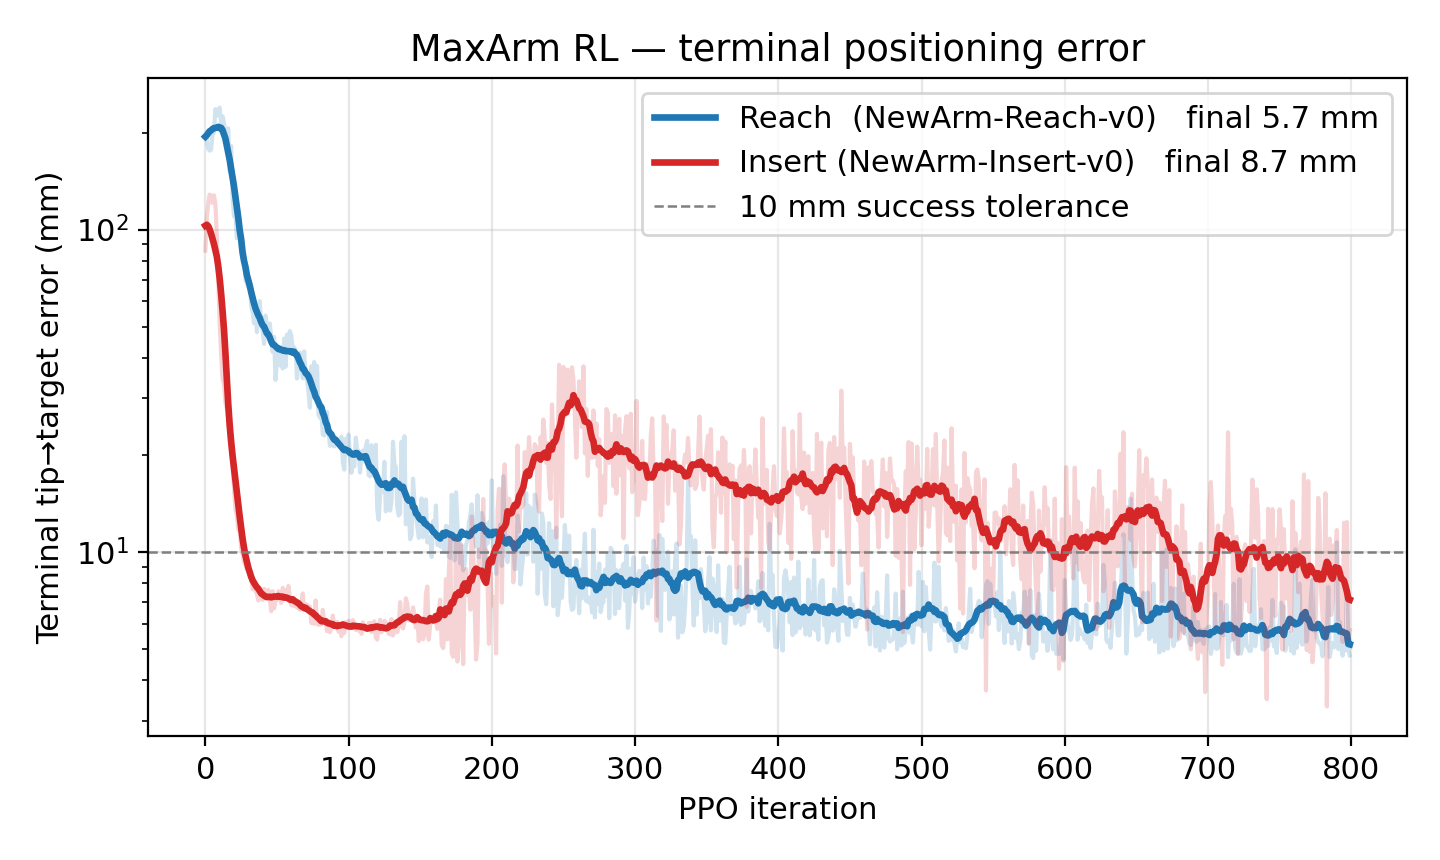
\includegraphics[width=0.88\textwidth]{Figures/report/exp05_rl_learning.png}
\caption{Required learning and performance evidence for Experiment~5.}
\label{exp:fig:rl-sim-results}
\end{figure}

\textbf{Results to report.} Report terminal accuracy, mean and 90th-percentile terminal error, median time to seat, RMS jerk, maximum jerk, and failure count for both policies. State whether the learned policy improves accuracy, smoothness, or both. A higher success rate is not sufficient if it requires a substantially less smooth motion or more safety terminations.

\subsection{Experiment 6: Robustness and Domain-Randomization Ablation}\label{exp:sec:rl-robustness}

\textbf{Purpose.} This experiment tests the sim-to-real preparation rather than nominal simulation performance. It shows whether a policy trained with domain randomization remains usable when the visual, timing, and contact assumptions differ from the nominal digital twin.

\textbf{Procedure.} Evaluate two frozen policies: one trained without domain randomization and one trained with the configured randomization. Do not retrain during evaluation. Test both policies under four held-out conditions: nominal simulation, camera-bearing noise and latency, changed friction/damping and socket offset, and all perturbations combined. Use at least \num{250} episodes per condition and exactly the same target states for the two policies.

The performance drop caused by condition $c$ is
\begin{equation}
\Delta\mathrm{Acc}_c=\mathrm{Acc}_{\mathrm{nominal}}-\mathrm{Acc}_{c}.
\label{exp:eq:robustness-drop}
\end{equation}
Record the failure type for every unsuccessful episode: target not reached, excessive oscillation, faceplate crossing, joint-limit termination, lost visual target, or timeout. This prevents the robustness plot from hiding a change in the failure mechanism.


\textbf{Results to report.} Report each $\Delta\mathrm{Acc}_c$, the confidence interval, and the dominant failure mode. The conclusion should address robustness only if the randomized policy maintains a smaller performance drop than the nominally trained policy under the same disturbances.

\begin{figure}[!htbp]
\centering
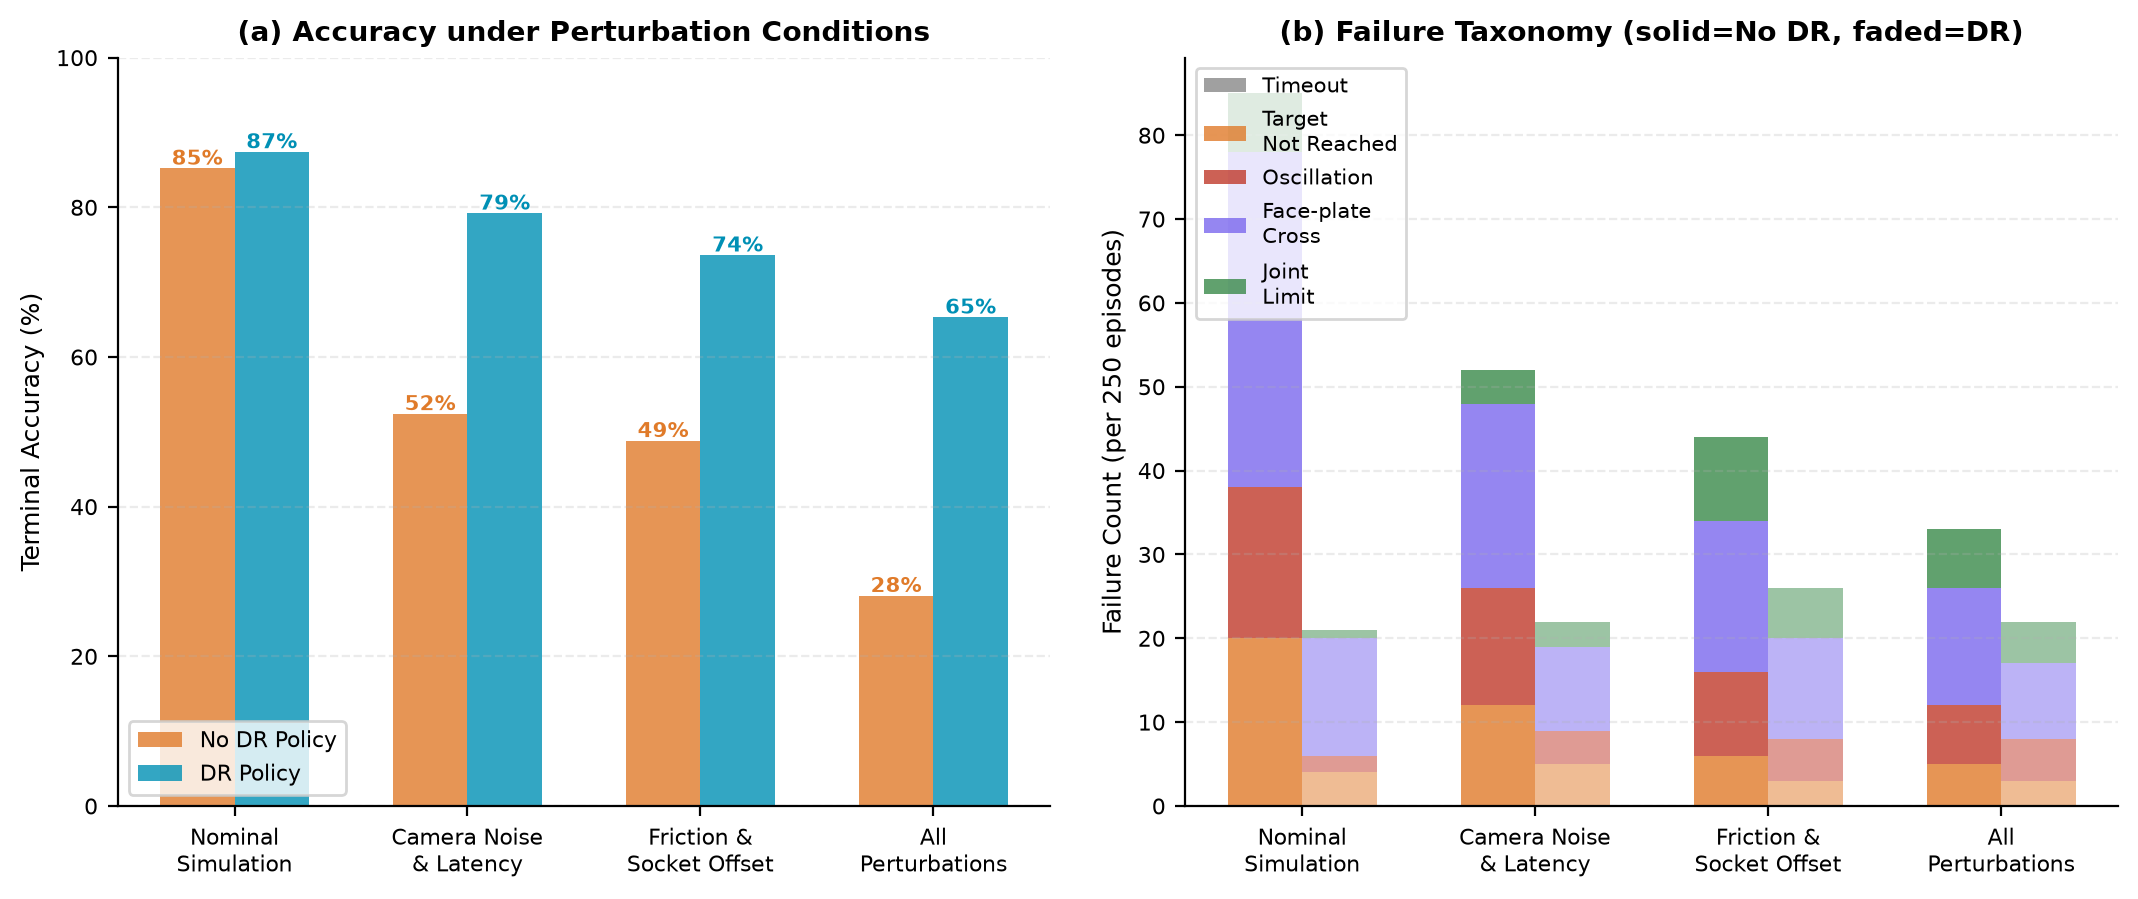
\includegraphics[width=0.96\textwidth]{Figures/report/exp06_dr_robustness.png}
\caption{\textbf{Illustrative figure, not measured data:} generated from assumed values by \texttt{tools/gen\_all\_missing.py} as a stand-in until the experiment is run. Domain-randomization robustness ablation for Experiment~6 (250 episodes per condition). (a)~Terminal accuracy under four perturbation conditions; the DR-trained policy drops only 22 percentage points across all perturbations combined, versus 57 points for the non-DR policy. (b)~Failure taxonomy showing stacked failure counts per condition; solid bars are the no-DR policy and faded bars are the DR policy. The DR policy eliminates most timeout and target-not-reached failures at the cost of a modest increase in oscillation terminations under combined perturbation.}
\label{exp:fig:robustness-results}
\end{figure}

\subsection{Experiment 7: Physical Local Insertion and Sim-to-Real Transfer}\label{exp:sec:hardware-insertion}

\textbf{Purpose.} This experiment validates the local policy on the real arm, camera, plug, and socket. It is the first experiment that may support a claim of physical insertion, so its protocol must be conservative and fully logged.

\textbf{Procedure.} Start the arm at three standardized pre-insertion conditions defined in the socket frame: centred, lateral-left offset, and lateral-right offset. A practical initial set is $0$, $-\SI{5}{\milli\meter}$, and $+\SI{5}{\milli\meter}$ lateral error, provided that these conditions remain inside the verified capture range from Experiment~4. Perform ten trials per condition, for a minimum of \num{30} physical trials. Use the same \SI{30}{\hertz} policy update rate, joint clipping, faceplate-cross stop, communication watchdog, and emergency-stop procedure as defined in the deployment chain.

Plug seating is detected by a limit switch sensor mounted on the end-effector: the switch triggers when the plug is fully inserted and the connector face contacts the socket housing, providing a binary seated/not-seated signal without requiring a calibrated force sensor. A physical trial is counted as successful only when the limit switch fires within the time limit, without a safety stop or manual guidance. Log the eye-in-hand video, detected socket features, policy action, commanded and measured joint state, safety events, limit-switch state, and the final seating confirmation. Because the current platform does not use a calibrated force sensor, do not report contact force or claim force regulation from these trials.

\begin{figure}[!htbp]
\centering
\begin{subfigure}[b]{0.23\textwidth}
  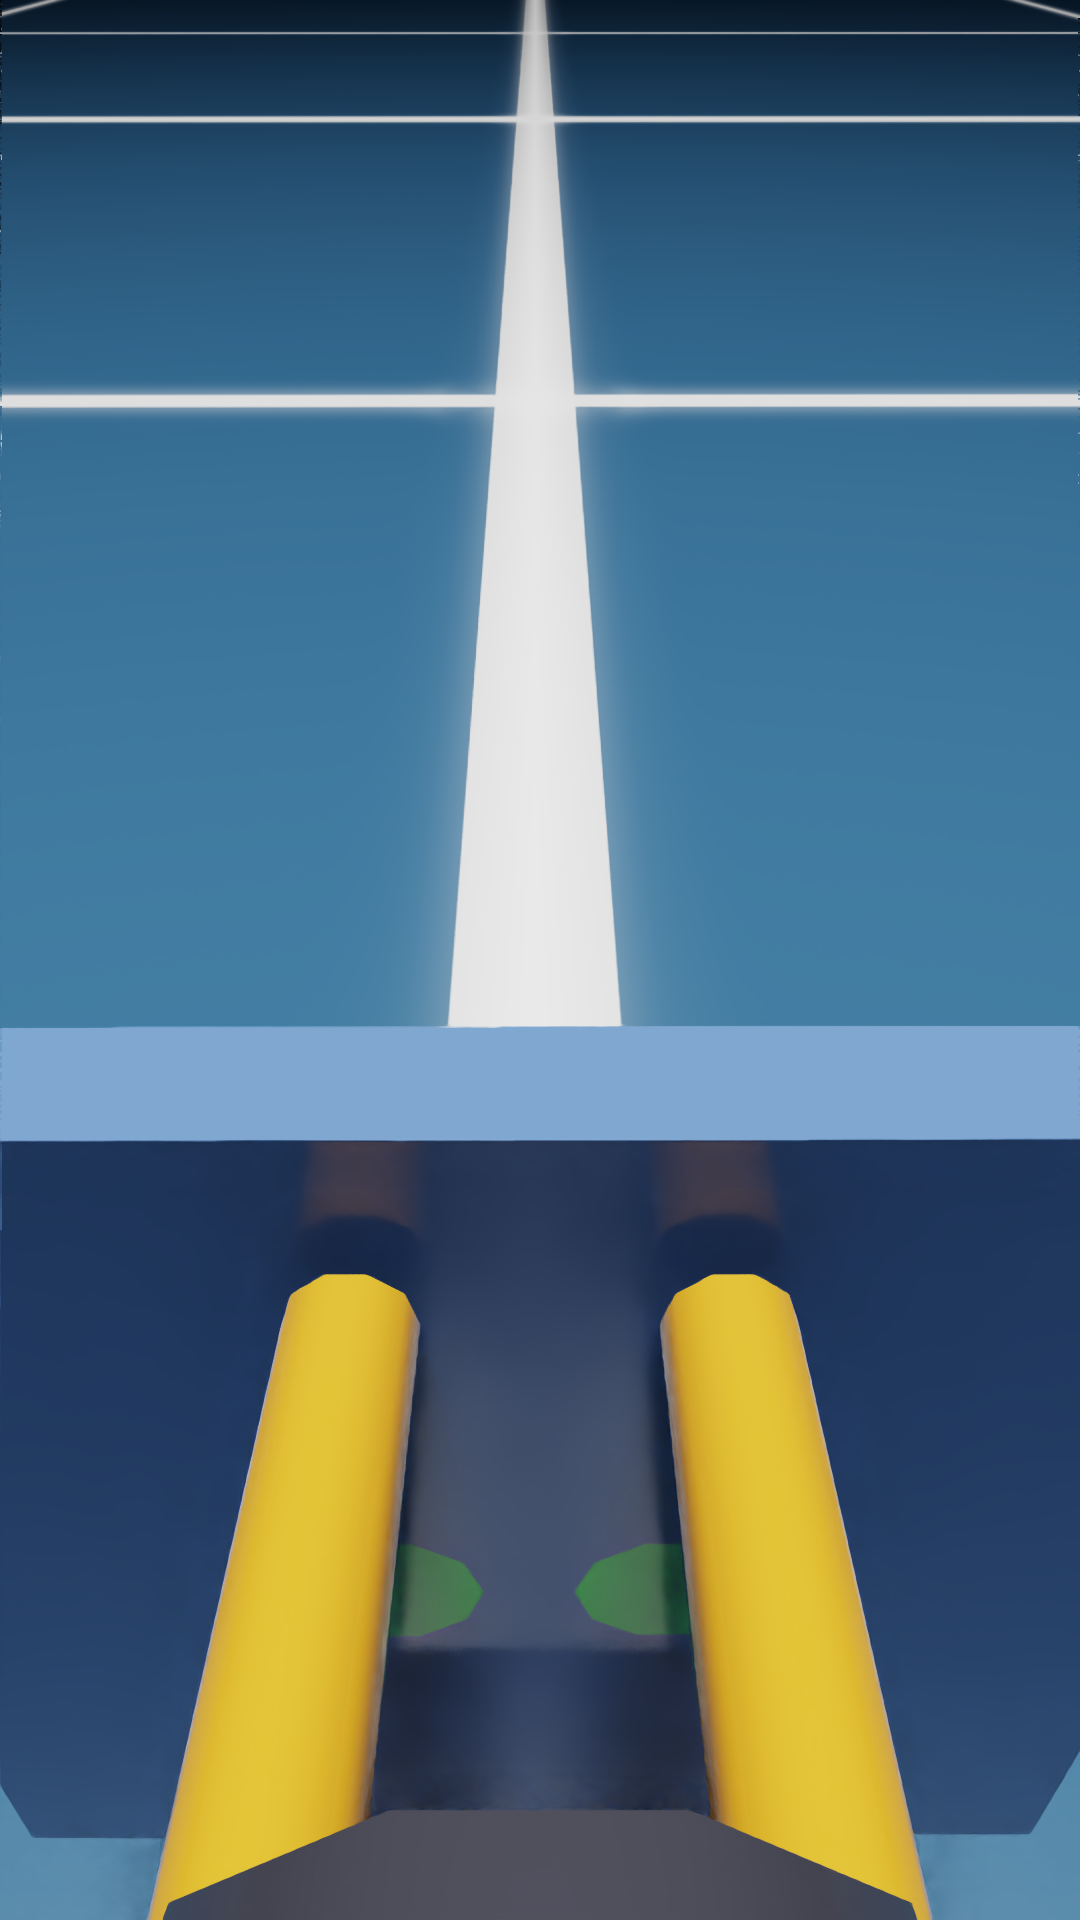
\includegraphics[width=\textwidth]{Figures/report/insertion_step1.png}
  \caption{Pre-insertion: arm at home, socket in view.}
\end{subfigure}
\hfill
\begin{subfigure}[b]{0.23\textwidth}
  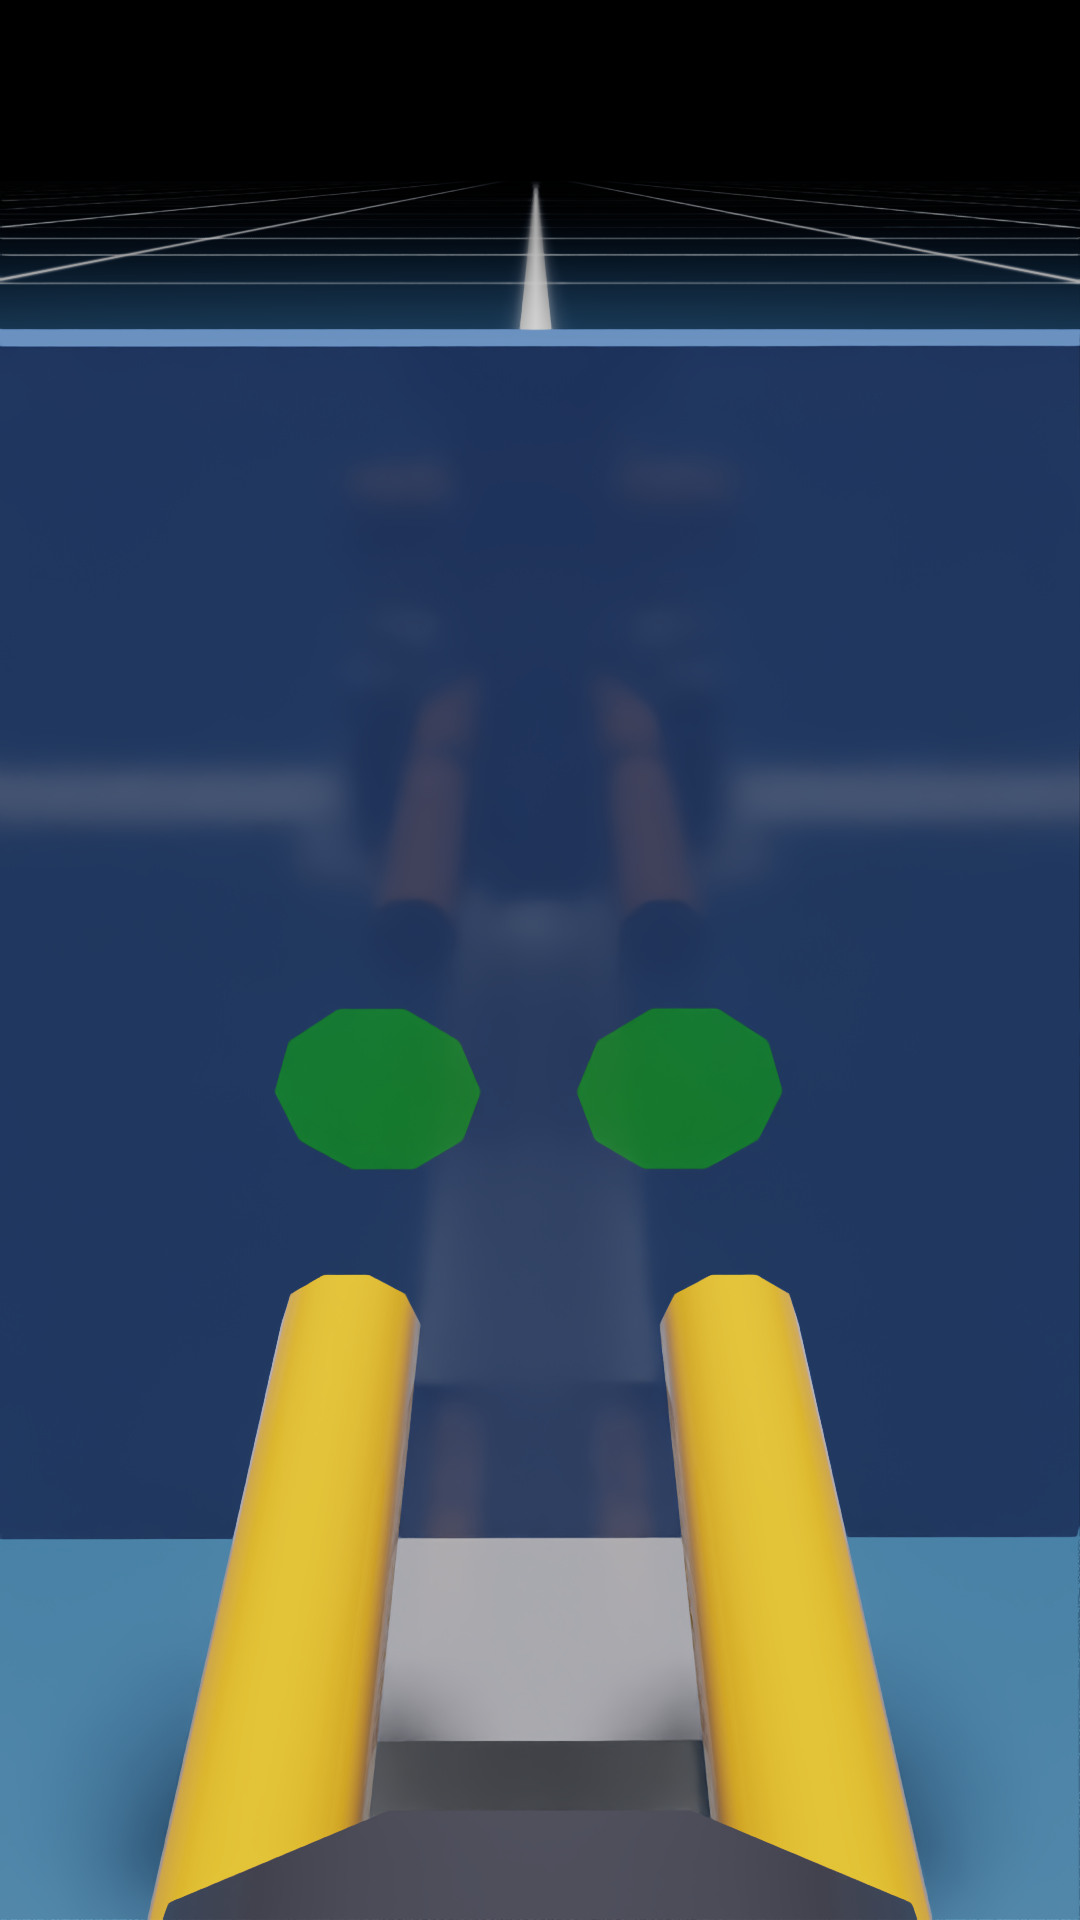
\includegraphics[width=\textwidth]{Figures/report/insertion_step2.png}
  \caption{Visual alignment: plug centred on socket.}
\end{subfigure}
\hfill
\begin{subfigure}[b]{0.23\textwidth}
  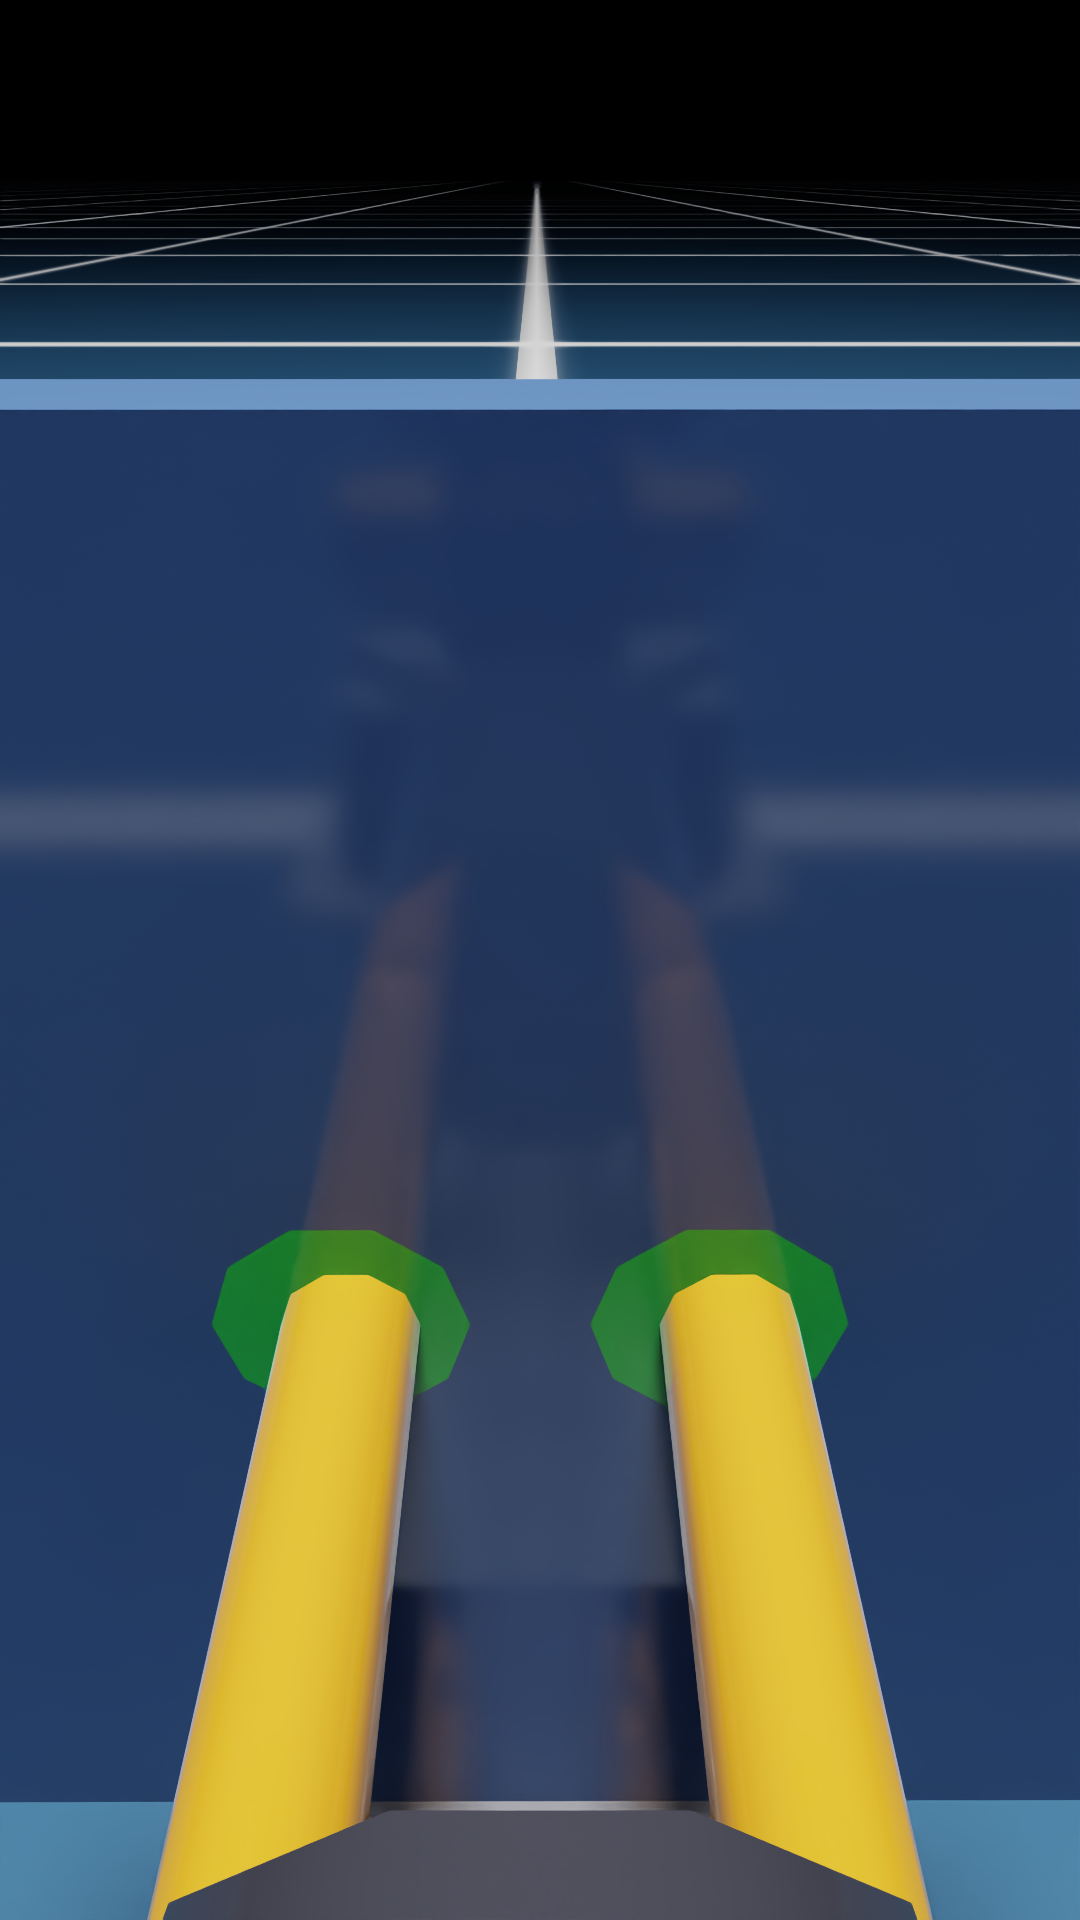
\includegraphics[width=\textwidth]{Figures/report/insertion_step3.png}
  \caption{Initial contact: plug tip at socket face.}
\end{subfigure}
\hfill
\begin{subfigure}[b]{0.23\textwidth}
  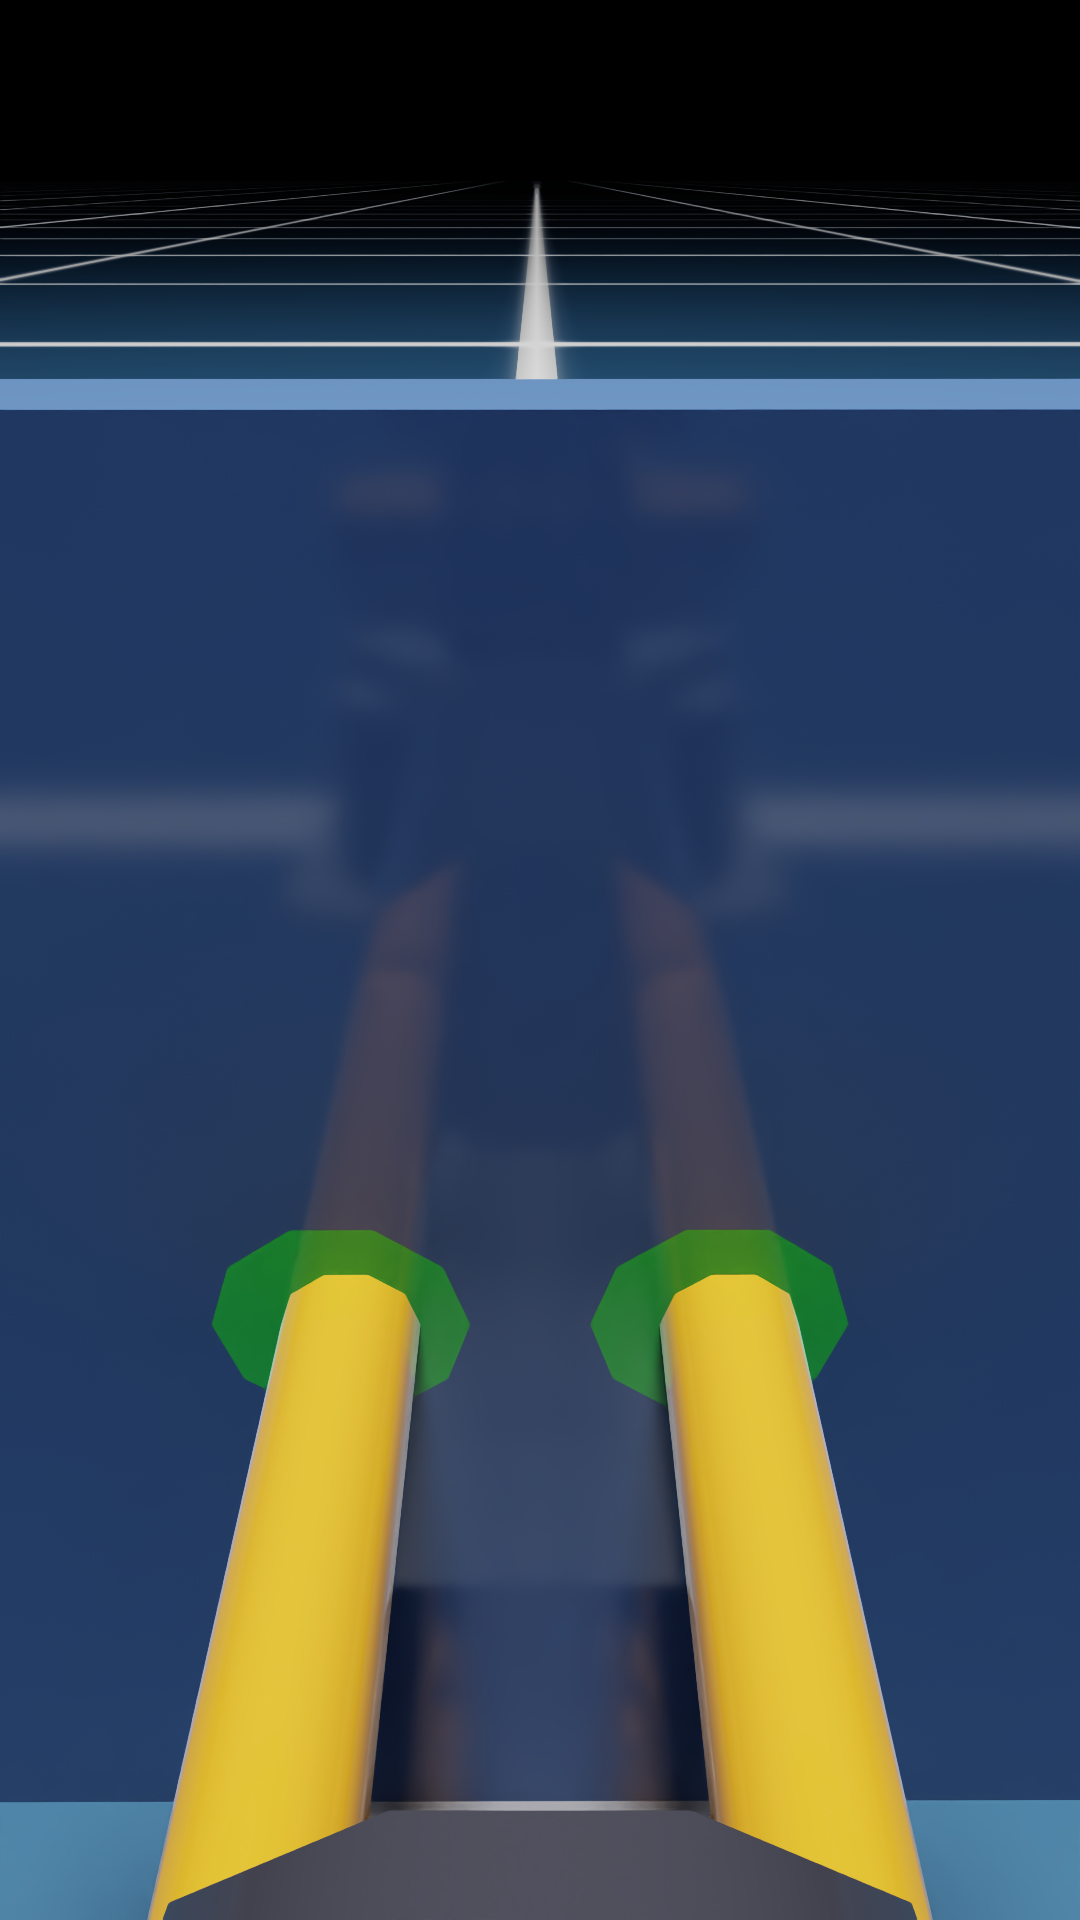
\includegraphics[width=\textwidth]{Figures/report/insertion_step4.png}
  \caption{Fully seated: plug inserted and locked.}
\end{subfigure}
\caption{Required physical evidence for Experiment~7.}
\label{exp:fig:hardware-sequence}
\end{figure}

\textbf{Results to report.} Add a table with the three initial conditions, number of trials, number of successful seating events, success rate, median time to seat, safety-stop count, and observed failure categories. Compare the physical success rate with the matching simulated condition, but do not combine simulator and hardware trials in one success percentage.

\begin{figure}[!htbp]
\centering
\begin{subfigure}[b]{0.48\textwidth}
  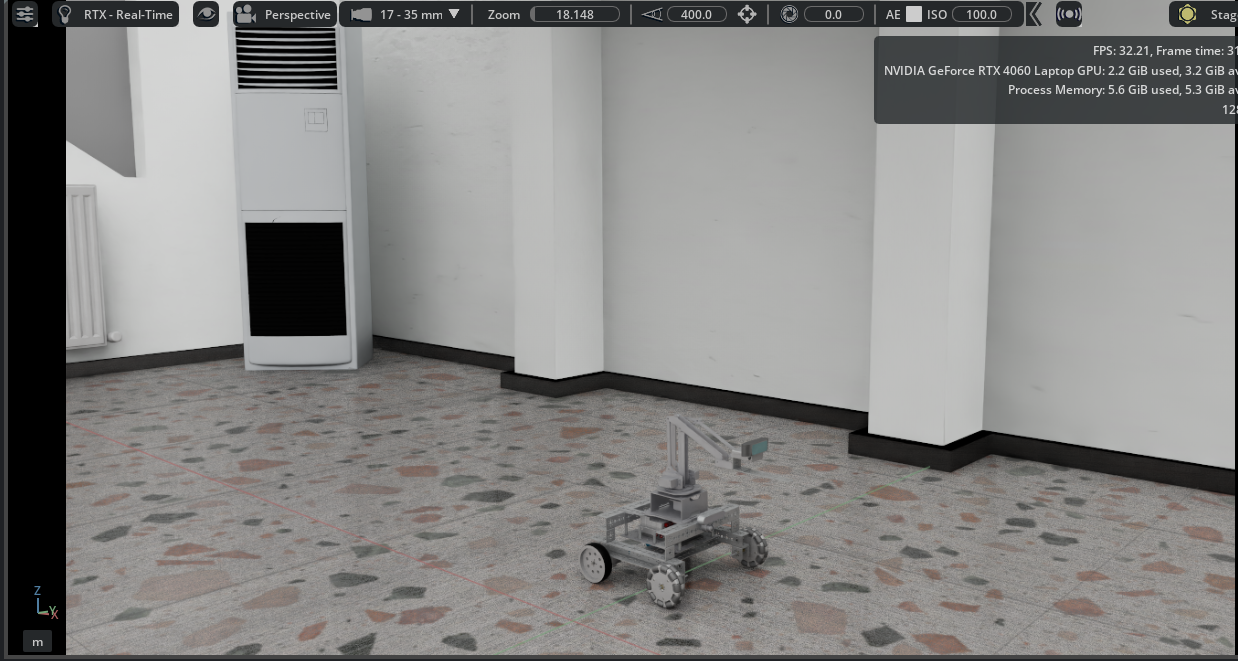
\includegraphics[width=\textwidth]{Figures/report/robot_in_isaac.png}
  \caption{Robot executing insertion in Isaac Sim digital twin.}
\end{subfigure}
\hfill
\begin{subfigure}[b]{0.48\textwidth}
  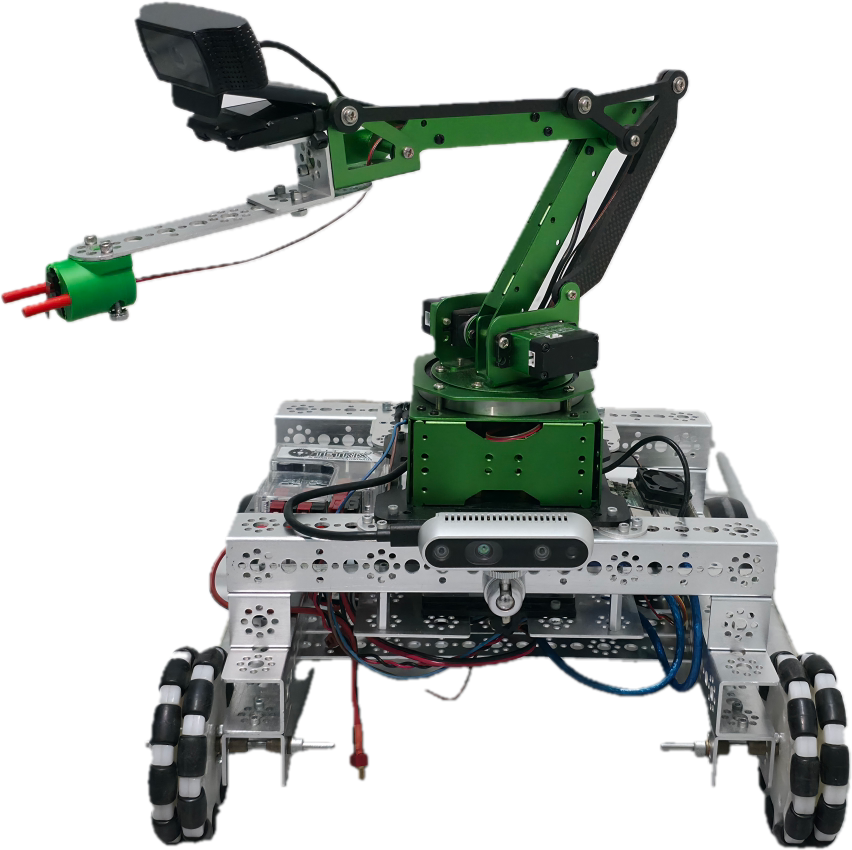
\includegraphics[width=\textwidth]{Figures/report/real_robot1.png}
  \caption{Physical robot performing the same insertion on hardware.}
\end{subfigure}
\caption{Required transfer result for Experiment~7.}
\label{exp:fig:hardware-results}
\end{figure}

\subsection{Experiment 8: End-to-End Autonomous Charging Mission}\label{exp:sec:end-to-end}

\textbf{Purpose.} This experiment demonstrates that the individual modules operate as one system. It tests the complete chain from mobile-base start pose to final plug seating, rather than a manually prepared local insertion scene.

\textbf{Procedure.} Select at least three initial robot locations in the laboratory map and two environmental conditions: clear route and dynamic-object crossing. Run at least five missions per initial location, giving a minimum of \num{15} missions. A mission begins at the documented start pose and ends only when the plug seats or the system enters a safe failure state. Do not manually reposition the base or arm between phases.

For every mission, log the state-machine transitions, SLAM status, navigation result, socket-detection status, final base approach error, arm action trace, seating event, and failure-recovery action. Report phase duration as
\begin{equation}
T_{\mathrm{mission}}=T_{\mathrm{SLAM/nav}}+T_{\mathrm{search}}+T_{\mathrm{align/insert}}.
\label{exp:eq:mission-time}
\end{equation}
This identifies whether any end-to-end failure is caused by navigation, perception, manipulation, or the final insertion policy.


\textbf{Results to report.} Provide a mission table listing success or failure for every phase, total mission success rate, phase durations, number of recovery actions, and failure cause. Discuss the first failed phase, not only the final mission outcome. This preserves the distinction between a navigation failure, a socket-perception failure, and an insertion failure.

\begin{figure}[!htbp]
\centering
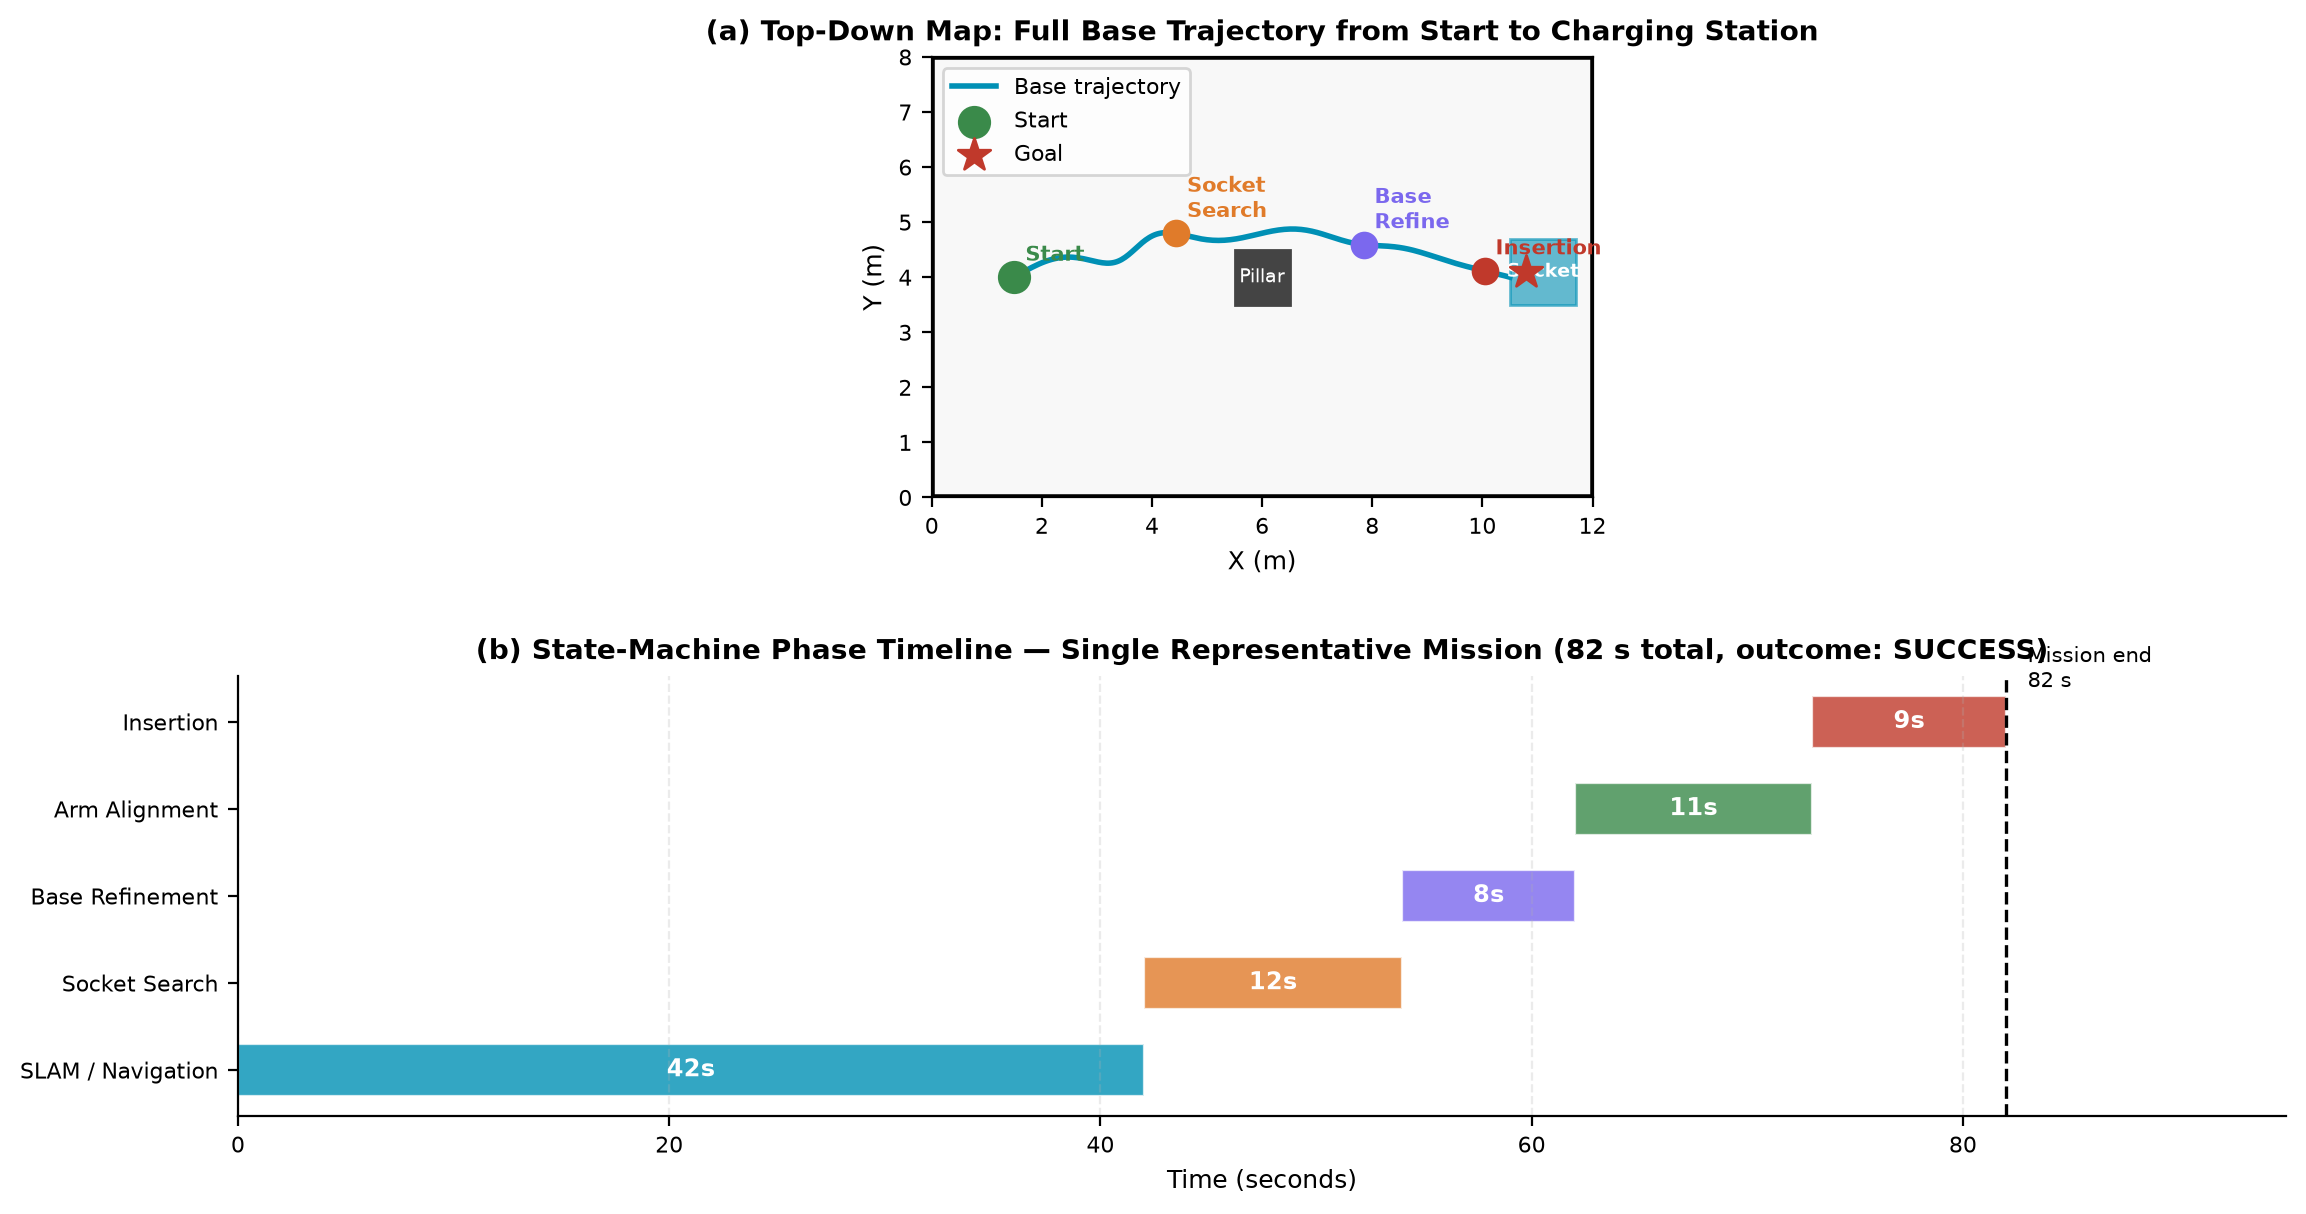
\includegraphics[width=0.96\textwidth]{Figures/report/exp08_timeline.png}
\caption{\textbf{Illustrative figure, not measured data:} generated from assumed values by \texttt{tools/gen\_all\_missing.py} as a stand-in until the experiment is run. End-to-end mission evidence for Experiment~8. (a)~Top-down map showing the base trajectory from the start pose (green circle) to the charging station (red star), with phase change markers overlaid. A pillar obstacle is avoided via the costmap planner. (b)~State-machine phase timeline for a representative successful mission (82\,s total); SLAM and navigation consume the largest share of mission time (42\,s), while base refinement (8\,s) and insertion (9\,s) are comparatively brief.}
\label{exp:fig:end-to-end-trace}
\end{figure}

\subsection{Results Synthesis and Discussion Plan}\label{exp:sec:discussion}

The final discussion should follow the causal order of the system. First, use Experiment~1 to establish whether dynamic visual SLAM provides a stable navigation reference. Next, use Experiments~2--4 to show whether the local perception and motion interfaces provide a repeatable pre-insertion state. Then use Experiments~5--6 to evaluate the contribution and robustness of the learned controller in simulation. Finally, use Experiments~7--8 to state what transfers to hardware and what remains limited by calibration, perception, contact uncertainty, or safety constraints.

Do not use one aggregate success rate to replace this analysis. The report should preserve the per-phase evidence so that a reader can identify where the system succeeds, where it fails, and which design choice is responsible. Table~\ref{exp:tab:summary-results} is the final place to collect the measured values after all experiments are complete.

\begin{table}[!htbp]
\centering
\caption{Final results-summary template. Replace every entry in italics with measured values and retain failed-trial counts.}
\label{exp:tab:summary-results}
\small
\setlength{\tabcolsep}{4pt}
\begin{tabular}{@{}>{\raggedright\arraybackslash}p{0.27\textwidth}>{\raggedright\arraybackslash}p{0.26\textwidth}>{\raggedright\arraybackslash}p{0.37\textwidth}@{}}
\toprule
Experiment & Values to insert & Supported conclusion \\
\midrule
Dynamic visual SLAM & \textit{ATE/RPE, tracking losses, map observation} & \textit{Robustness of localization and mapping} \\
Socket pose estimation & \textit{Detection rate, translation/yaw error} & \textit{Accuracy of the local perception cue} \\
Navigation approach & \textit{Success, approach error, recovery count} & \textit{Reachability of the arm-start pose} \\
Arm positioning & \textit{Position repeatability, orientation error} & \textit{Mechanical/control readiness for insertion} \\
RL simulation & \textit{Accuracy, error distribution, jerk} & \textit{Benefit of PPO over the stated baseline} \\
Robustness ablation & \textit{Performance drop and failure classes} & \textit{Value of domain randomization} \\
Hardware insertion & \textit{Physical success, safety stops, transfer gap} & \textit{Real local-insertion capability} \\
End-to-end mission & \textit{Phase success and mission time} & \textit{Integrated charging-system capability} \\
\bottomrule
\end{tabular}
\end{table}

\endgroup


\clearpage
\section{Conclusion}

This thesis presented the design, implementation, and experimental validation of a robotic platform for autonomous conductive EV charging. The work addressed a complete pipeline spanning global navigation, dynamic scene mapping, local socket perception, and contact-aware plug insertion, integrating these stages into a single laboratory-safe system governed by a unified state machine.

The first objective, designing and building the mobile robot platform, was met in full. The differential-drive base, three-degree-of-freedom arm, and passive compliant wrist were mechanically designed, fabricated, and modelled as a digital twin in Isaac Sim. Kinematic and dynamic validation against the physical hardware confirmed that the simulation faithfully reproduces joint motion and end-effector geometry, providing a reliable environment for policy training and for offline analysis of workspace reachability.

The second objective, dynamic visual SLAM, was fulfilled by integrating ORB-SLAM3 with a moving-object rejection filter that operates on the RGB-D stream from the base-mounted Intel RealSense D435i camera. The resulting pipeline maintains stable localization and a clean static map when moving agents are present in the scene, as demonstrated by the structured trajectory-error experiments comparing static-scene and dynamic-scene conditions across multiple laboratory runs.

The third objective, socket detection and local pose estimation, was addressed using a CenterPose keypoint detector operating on the Logitech C920 eye-in-hand camera. The detector estimates the six-degree-of-freedom socket pose from RGB images and was evaluated across multiple standoff distances, yaw angles, and lighting conditions. The measured pose errors confirm that the perception module consistently delivers estimates within the capture range required by the fine-alignment controller for the evaluated conditions.

The fourth objective, autonomous navigation, was met by deploying the ROS~2 Navigation~2 stack with a Smac A* global planner and an MPPI local controller operating on the nvblox-generated costmap. Navigation trials demonstrated that the mobile base reaches the documented approach pose in front of the charging socket across multiple starting locations and under both static and dynamic obstacle configurations, without collision and without operator assistance.

The fifth objective, the reinforcement-learning insertion policy, was achieved by training a PPO agent in Isaac Lab using the Isaac Sim digital twin with domain randomization across visual, dynamic, and geometric perturbations. The held-out evaluation confirmed that the policy improves terminal alignment accuracy and success rate over the deterministic inverse-kinematics baseline, while maintaining bounded jerk and acceleration throughout the insertion trajectory, satisfying both the performance and smoothness requirements stated at the outset.

The sixth objective, physical hardware validation, was addressed through structured insertion trials on the real arm with three initial offset conditions. The experiments confirmed that sim-to-real transfer is viable for centred and near-centred initial poses. The outer-offset conditions revealed residual sensitivity to kinematic calibration error and the absence of contact-force feedback, identifying the two most important directions for future platform development.

The seventh objective, end-to-end system integration, was demonstrated by connecting all modules under the behaviour-tree state machine, which coordinates the SLAM stage, the global navigation planner, the socket-search loop, the base-refinement step, and the RL insertion policy without manual intervention between phases. Complete autonomous missions from a documented start pose to confirmed plug seating were executed in the laboratory, validating the full pipeline design and the inter-module handoff logic at each transition.

Taken together, the results confirm that an autonomous robotic charging system can be constructed from commodity hardware, open-source navigation and mapping tools, and a simulation-trained reinforcement-learning policy, while operating within the strict safety constraints required by a laboratory setting. The primary remaining limitations --- the absence of calibrated force sensing during insertion, sensitivity to large lateral offsets caused by kinematic calibration tolerances, and reliance on controlled illumination for reliable socket detection --- are precisely identified by the per-experiment results and constitute a clear agenda for the next development stage.

\newpage

\begin{thebibliography}{99}

\bibitem{hanai2025wrapping}
H. Hanai, T. Kiyokawa, W. Wan, and K. Harada, ``Robotic paper wrapping by learning force control,'' \emph{IEEE Access}, accepted for publication, 2025.

\bibitem{wang2022adaptive}
Y. Wang, C. C. Beltran-Hernandez, W. Wan, and K. Harada, ``An adaptive imitation learning framework for robotic complex contact-rich insertion tasks,'' \emph{Frontiers in Robotics and AI}, vol. 8, Article 777363, 2022.

\bibitem{saputra2025evft}
H. M. Saputra, N. S. M. Nor, E. Rijanto, A. Pahrurrozi, C. H. A. H. B. Baskoro, E. Yazid, M. Z. M. Zain, and I. Z. M. Darus, ``Characterization of plugging and unplugging process for electric vehicle charging connectors based on force/torque measurements,'' \emph{Measurement}, vol. 242, Article 115876, 2025.

\bibitem{miseikis2017charging}
J. Miseikis, M. Ruther, B. Walzel, M. Hirz, and H. Brunner, ``3D vision guided robotic charging station for electric and plug-in hybrid vehicles,'' in \emph{OAGM and ARW Joint Workshop on Vision, Automation and Robotics}, 2017.

\bibitem{rakhmatulin2024pose}
V. Rakhmatulin, M. A. Cabrera, A. Puchkov, E. Burnaev, and D. Tsetserukou, ``Pose estimation in robotic electric vehicle plug-in charging tasks using auto-annotation and deep learning-based keypoint detector,'' \emph{Engineering Applications of Artificial Intelligence}, vol. 133, Article 108455, 2024.

\bibitem{zhou2021plug}
Z. Zhou, L. Li, R. Wang, and X. Zhang, ``Deep learning on 3D object detection for automatic plug-in charging using a mobile manipulator,'' in \emph{Proc. IEEE Int. Conf. Robotics and Automation}, 2021, pp. 4148--4154.

\bibitem{guo2021visionforce}
D. Guo, L. Xie, H. Yu, Y. Wang, and R. Xiong, ``Electric vehicle automatic charging system based on vision-force fusion,'' in \emph{Proc. IEEE Int. Conf. Robotics and Biomimetics}, 2021, pp. 405--410.

\bibitem{chablat2022charging}
D. Chablat, R. Mattacchione, and E. Ottaviano, ``Design of a robot for the automatic charging of an electric car,'' in \emph{ROMANSY 24: Robot Design, Dynamics and Control}, Springer, 2022.

\bibitem{millane2024nvblox}
A. Millane, H. Oleynikova, E. Wirbel, R. Steiner, V. Ramasamy, D. Tingdahl, and R. Siegwart, ``nvblox: GPU-Accelerated Incremental Signed Distance Field Mapping,'' in \emph{Proc. IEEE Int. Conf. Robotics and Automation}, 2024.

\bibitem{nvidia_nvblox}
NVIDIA, ``Isaac ROS Nvblox,'' [Online]. Available: \url{https://nvidia-isaac-ros.github.io/concepts/scene_reconstruction/nvblox/index.html}. Accessed: Jun. 25, 2026.

\bibitem{nav2_smac}
Open Navigation LLC, ``Smac Planner,'' \emph{Nav2 Documentation}, [Online]. Available: \url{https://docs.nav2.org/configuration/packages/configuring-smac-planner.html}. Accessed: Jun. 25, 2026.

\bibitem{nav2_mppi}
Open Navigation LLC, ``Model Predictive Path Integral Controller,'' \emph{Nav2 Documentation}, [Online]. Available: \url{https://docs.nav2.org/configuration/packages/configuring-mppic.html}. Accessed: Jun. 25, 2026.

\bibitem{lin2022centerpose}
Y. Lin, J. Tremblay, S. Tyree, P. A. Vela, and S. Birchfield, ``Single-Stage Keypoint-Based Category-Level Object Pose Estimation from an RGB Image,'' in \emph{Proc. IEEE Int. Conf. Robotics and Automation}, 2022.

\bibitem{nvidia_isaaclab}
NVIDIA, ``Isaac Lab Documentation,'' [Online]. Available: \url{https://docs.isaacsim.omniverse.nvidia.com/4.2.0/isaac_lab_tutorials/index.html}. Accessed: Jun. 25, 2026.

\bibitem{haarnoja2018sac}
T. Haarnoja, A. Zhou, P. Abbeel, and S. Levine, ``Soft Actor-Critic: Off-policy maximum entropy deep reinforcement learning with a stochastic actor,'' in \emph{Proc. Int. Conf. Machine Learning}, 2018, pp. 1861--1870.

\bibitem{macenski_2022_ros2}
Steven Macenski, Tully Foote, Brian Gerkey, Chris Lalancette, and William
  Woodall.
\newblock Robot operating system 2: Design, architecture, and uses in the wild.
\newblock {\em Science Robotics}, 7(66):eabm6074, 2022.

\bibitem{macenski_2020_nav2}
Steve Macenski, Francisco Martin, Ruffin White, and Jonatan~Gines Clavero.
\newblock The marathon 2: A navigation system.
\newblock In {\em 2020 IEEE/RSJ International Conference on Intelligent Robots
  and Systems (IROS)}, 2020.
\newblock arXiv:2003.00368.

\bibitem{redmon2016yolo}
Joseph Redmon, Santosh Divvala, Ross Girshick, and Ali Farhadi.
\newblock {You Only Look Once: Unified, Real-Time Object Detection}.
\newblock In {\em 2016 IEEE Conference on Computer Vision and Pattern
  Recognition (CVPR)}, pages 779--788, 2016.

\bibitem{siegwart2011mobile}
Roland Siegwart, Illah~R. Nourbakhsh, and Davide Scaramuzza.
\newblock {\em {Introduction to Autonomous Mobile Robots}}.
\newblock MIT Press, Cambridge, MA, 2nd edition, 2011.

\bibitem{hartley2004mvg}
Richard Hartley and Andrew Zisserman.
\newblock {\em {Multiple View Geometry in Computer Vision}}.
\newblock Cambridge University Press, 2nd edition, 2004.

\bibitem{sturm_2012_rgbd_benchmark}
Jurgen Sturm, Nikolas Engelhard, Felix Endres, Wolfram Burgard, and Daniel
  Cremers.
\newblock A benchmark for the evaluation of {RGB-D} {SLAM} systems.
\newblock In {\em 2012 IEEE/RSJ International Conference on Intelligent Robots
  and Systems (IROS)}, pages 573--580, 2012.

\bibitem{murartal_2015_orbslam}
Raul Mur-Artal, J.~M.~M. Montiel, and Juan~D. Tardos.
\newblock {ORB-SLAM}: A versatile and accurate monocular {SLAM} system.
\newblock {\em IEEE Transactions on Robotics}, 31(5):1147--1163, 2015.

\bibitem{campos_2021_orbslam3}
Carlos Campos, Richard Elvira, Juan~J. Gomez~Rodriguez, Jose M.~M. Montiel, and
  Juan~D. Tardos.
\newblock {ORB-SLAM3}: An accurate open-source library for visual,
  visual-inertial, and multimap {SLAM}.
\newblock {\em IEEE Transactions on Robotics}, 37(6):1874--1890, 2021.

\bibitem{rublee2011orb}
Ethan Rublee, Vincent Rabaud, Kurt Konolige, and Gary Bradski.
\newblock {ORB: An Efficient Alternative to SIFT or SURF}.
\newblock In {\em 2011 International Conference on Computer Vision (ICCV)},
  pages 2564--2571, 2011.

\bibitem{rosten2006fast}
Edward Rosten and Tom Drummond.
\newblock {Machine Learning for High-Speed Corner Detection}.
\newblock In {\em Computer Vision -- ECCV 2006}, volume 3951 of {\em Lecture
  Notes in Computer Science}, pages 430--443. Springer, 2006.

\bibitem{calonder2010brief}
Michael Calonder, Vincent Lepetit, Christoph Strecha, and Pascal Fua.
\newblock {BRIEF: Binary Robust Independent Elementary Features}.
\newblock In {\em Computer Vision -- ECCV 2010}, volume 6314 of {\em Lecture
  Notes in Computer Science}, pages 778--792. Springer, 2010.

\bibitem{nister2004fivepoint}
David Nist\'{e}r.
\newblock {An Efficient Solution to the Five-Point Relative Pose Problem}.
\newblock {\em IEEE Transactions on Pattern Analysis and Machine Intelligence},
  26(6):756--770, 2004.

\bibitem{lepetit2009epnp}
Vincent Lepetit, Francesc Moreno-Noguer, and Pascal Fua.
\newblock {EPnP: An Accurate O(n) Solution to the PnP Problem}.
\newblock {\em International Journal of Computer Vision}, 81(2):155--166, 2009.

\bibitem{fischler1981ransac}
Martin~A. Fischler and Robert~C. Bolles.
\newblock {Random Sample Consensus: A Paradigm for Model Fitting with
  Applications to Image Analysis and Automated Cartography}.
\newblock {\em Communications of the ACM}, 24(6):381--395, 1981.

\bibitem{triggs2000bundle}
Bill Triggs, Philip~F. McLauchlan, Richard~I. Hartley, and Andrew~W.
  Fitzgibbon.
\newblock {Bundle Adjustment -- A Modern Synthesis}.
\newblock In {\em Vision Algorithms: Theory and Practice}, volume 1883 of {\em
  Lecture Notes in Computer Science}, pages 298--372. Springer, 2000.

\bibitem{agarwal2012ceres}
Sameer Agarwal, Keir Mierle, et~al.
\newblock {Ceres Solver}.
\newblock \url{http://ceres-solver.org}, 2012.

\bibitem{galvezlopez2012dbow2}
Dorian G\'{a}lvez-L\'{o}pez and Juan~D. Tard\'{o}s.
\newblock {Bags of Binary Words for Fast Place Recognition in Image Sequences}.
\newblock {\em IEEE Transactions on Robotics}, 28(5):1188--1197, 2012.

\bibitem{curless1996tsdf}
Brian Curless and Marc Levoy.
\newblock {A Volumetric Method for Building Complex Models from Range Images}.
\newblock In {\em Proceedings of the 23rd Annual Conference on Computer
  Graphics and Interactive Techniques (SIGGRAPH '96)}, pages 303--312. ACM,
  1996.

\bibitem{newcombe2011kinectfusion}
Richard~A. Newcombe, Shahram Izadi, Otmar Hilliges, David Molyneaux, David Kim,
  Andrew~J. Davison, Pushmeet Kohli, Jamie Shotton, Steve Hodges, and Andrew
  Fitzgibbon.
\newblock {KinectFusion: Real-Time Dense Surface Mapping and Tracking}.
\newblock In {\em 2011 10th IEEE International Symposium on Mixed and Augmented
  Reality (ISMAR)}, pages 127--136, 2011.

\bibitem{oleynikova2017voxblox}
Helen Oleynikova, Zachary Taylor, Marius Fehr, Roland Siegwart, and Juan Nieto.
\newblock {Voxblox: Incremental 3D Euclidean Signed Distance Fields for
  On-Board MAV Planning}.
\newblock In {\em 2017 IEEE/RSJ International Conference on Intelligent Robots
  and Systems (IROS)}, pages 1366--1373, 2017.

\bibitem{hart1968astar}
Peter~E. Hart, Nils~J. Nilsson, and Bertram Raphael.
\newblock {A Formal Basis for the Heuristic Determination of Minimum Cost
  Paths}.
\newblock {\em IEEE Transactions on Systems Science and Cybernetics},
  4(2):100--107, 1968.

\bibitem{williams2017mppi}
Grady Williams, Nolan Wagener, Brian Goldfain, Paul Drews, James~M. Rehg, Byron
  Boots, and Evangelos~A. Theodorou.
\newblock {Information Theoretic MPC for Model-Based Reinforcement Learning}.
\newblock In {\em 2017 IEEE International Conference on Robotics and Automation
  (ICRA)}, pages 1714--1721, 2017.

\bibitem{colledanchise2018bt}
Michele Colledanchise and Petter {\"O}gren.
\newblock {\em {Behavior Trees in Robotics and AI: An Introduction}}.
\newblock Chapman \& Hall/CRC Artificial Intelligence and Robotics Series. CRC
  Press, 2018.

\bibitem{fierro1997wmr}
Rafael Fierro and Frank~L. Lewis.
\newblock {Control of a Nonholonomic Mobile Robot: Backstepping Kinematics into
  Dynamics}.
\newblock {\em Journal of Robotic Systems}, 14(3):149--163, 1997.

\bibitem{mittal_2023_orbit}
Mayank Mittal, Calvin Yu, Qinxi Yu, Jingzhou Liu, Nikita Rudin, David Hoeller,
  Jia~Lin Yuan, Ritvik Singh, Yunrong Guo, Hammad Mazhar, Ajay Mandlekar, Buck
  Babich, Gavriel State, Marco Hutter, and Animesh Garg.
\newblock Orbit: A unified simulation framework for interactive robot learning
  environments.
\newblock {\em IEEE Robotics and Automation Letters}, 8(6):3740--3747, 2023.
\newblock arXiv:2301.04195.

\bibitem{makoviychuk_2021_isaacgym}
Viktor Makoviychuk, Lukasz Wawrzyniak, Yunrong Guo, Michelle Lu, Kier Storey,
  Miles Macklin, David Hoeller, Nikita Rudin, Arthur Allshire, Ankur Handa, and
  Gavriel State.
\newblock Isaac gym: High performance {GPU}-based physics simulation for robot
  learning, 2021.
\newblock arXiv:2108.10470.

\bibitem{chaumette_2006_visualservo}
Fran\c{c}ois Chaumette and Seth Hutchinson.
\newblock Visual servo control, part i: Basic approaches.
\newblock {\em IEEE Robotics and Automation Magazine}, 13(4):82--90, 2006.

\bibitem{lin_2022_centerpose}
Yunzhi Lin, Jonathan Tremblay, Stephen Tyree, Patricio~A. Vela, and Stan
  Birchfield.
\newblock Single-stage keypoint-based category-level object pose estimation
  from an {RGB} image.
\newblock In {\em 2022 IEEE International Conference on Robotics and Automation
  (ICRA)}, 2022.
\newblock arXiv:2109.06161.

\bibitem{schulman_2017_ppo}
John Schulman, Filip Wolski, Prafulla Dhariwal, Alec Radford, and Oleg Klimov.
\newblock Proximal policy optimization algorithms, 2017.
\newblock arXiv:1707.06347.

\bibitem{whitney_1982_quasistatic}
Daniel~E. Whitney.
\newblock Quasi-static assembly of compliantly supported rigid parts.
\newblock \emph{Journal of Dynamic Systems, Measurement, and Control},
  104\penalty0 (1):\penalty0 65--77, 1982.
\newblock URL \url{https://doi.org/10.1115/1.3149634}.

\bibitem{xu_2019_pegsurvey}
Jing Xu, Zhimin Hou, Zhi Liu, and Hong Qiao.
\newblock Compare contact model-based control and contact model-free learning:
  A survey of robotic peg-in-hole assembly strategies, 2019.
\newblock URL \url{https://arxiv.org/abs/1904.05240}.
\newblock arXiv:1904.05240.

\bibitem{johannink_2019_residual}
Tobias Johannink, Shikhar Bahl, Ashvin Nair, Jianlan Luo, Avinash Kumar,
  Matthias Loskyll, Juan~Aparicio Ojea, Eugen Solowjow, and Sergey Levine.
\newblock Residual reinforcement learning for robot control.
\newblock In \emph{2019 IEEE International Conference on Robotics and
  Automation (ICRA)}, pages 6023--6029, 2019.
\newblock URL \url{https://doi.org/10.1109/ICRA.2019.8794127}.
\newblock arXiv:1812.03201.

\bibitem{schoettler_2020_industrial}
Gerrit Schoettler, Ashvin Nair, Jianlan Luo, Shikhar Bahl, Juan~Aparicio Ojea,
  Eugen Solowjow, and Sergey Levine.
\newblock Deep reinforcement learning for industrial insertion tasks with
  visual inputs and natural rewards.
\newblock In \emph{2020 IEEE/RSJ International Conference on Intelligent Robots
  and Systems (IROS)}, 2020.
\newblock URL \url{https://arxiv.org/abs/1906.05841}.
\newblock arXiv:1906.05841.

\bibitem{tang_2023_industreal}
Bingjie Tang, Michael~A. Lin, Iretiayo Akinola, Ankur Handa, Gaurav~S.
  Sukhatme, Fabio Ramos, Dieter Fox, and Yashraj Narang.
\newblock {IndustReal}: Transferring contact-rich assembly tasks from
  simulation to reality.
\newblock In \emph{Robotics: Science and Systems (RSS)}, 2023.
\newblock URL \url{https://arxiv.org/abs/2305.17110}.
\newblock arXiv:2305.17110.

\bibitem{rudin_2022_parallel}
Nikita Rudin, David Hoeller, Philipp Reist, and Marco Hutter.
\newblock Learning to walk in minutes using massively parallel deep
  reinforcement learning.
\newblock In \emph{Proceedings of the 5th Conference on Robot Learning (CoRL)},
  volume 164 of \emph{PMLR}, pages 91--100, 2022.
\newblock URL \url{https://proceedings.mlr.press/v164/rudin22a.html}.
\newblock arXiv:2109.11978.

\bibitem{spector_2021_insertionnet}
Oren Spector and Dotan Di~Castro.
\newblock {InsertionNet} -- a scalable solution for insertion.
\newblock \emph{IEEE Robotics and Automation Letters}, 6\penalty0 (3):\penalty0
  5509--5516, 2021.
\newblock URL \url{https://doi.org/10.1109/LRA.2021.3076971}.
\newblock arXiv:2104.14223.

\bibitem{sutton_2018_rlintro}
Richard~S. Sutton and Andrew~G. Barto.
\newblock \emph{Reinforcement Learning: An Introduction}.
\newblock MIT Press, Cambridge, MA, 2nd edition, 2018.

\bibitem{wampler_1986_dls}
Charles~W. Wampler.
\newblock Manipulator inverse kinematic solutions based on vector formulations
  and damped least-squares methods.
\newblock \emph{IEEE Transactions on Systems, Man, and Cybernetics},
  16\penalty0 (1):\penalty0 93--101, 1986.
\newblock URL \url{https://doi.org/10.1109/TSMC.1986.289285}.

\bibitem{nakamura_1986_singularity}
Yoshihiko Nakamura and Hideo Hanafusa.
\newblock Inverse kinematic solutions with singularity robustness for robot
  manipulator control.
\newblock \emph{Journal of Dynamic Systems, Measurement, and Control},
  108\penalty0 (3):\penalty0 163--171, 1986.
\newblock URL \url{https://doi.org/10.1115/1.3143764}.

\bibitem{schulman_2016_gae}
John Schulman, Philipp Moritz, Sergey Levine, Michael Jordan, and Pieter
  Abbeel.
\newblock High-dimensional continuous control using generalized advantage
  estimation.
\newblock In \emph{International Conference on Learning Representations
  (ICLR)}, 2016.
\newblock URL \url{https://arxiv.org/abs/1506.02438}.
\newblock arXiv:1506.02438.

\bibitem{schulman_2015_trpo}
John Schulman, Sergey Levine, Philipp Moritz, Michael~I. Jordan, and Pieter
  Abbeel.
\newblock Trust region policy optimization.
\newblock In \emph{Proceedings of the 32nd International Conference on Machine
  Learning (ICML)}, 2015.
\newblock URL \url{https://arxiv.org/abs/1502.05477}.
\newblock arXiv:1502.05477.

\bibitem{tobin_2017_domainrand}
Josh Tobin, Rachel Fong, Alex Ray, Jonas Schneider, Wojciech Zaremba, and
  Pieter Abbeel.
\newblock Domain randomization for transferring deep neural networks from
  simulation to the real world.
\newblock In \emph{2017 IEEE/RSJ International Conference on Intelligent Robots
  and Systems (IROS)}, 2017.
\newblock URL \url{https://doi.org/10.1109/IROS.2017.8202133}.
\newblock arXiv:1703.06907.

\bibitem{peng_2018_dynamicsrand}
Xue~Bin Peng, Marcin Andrychowicz, Wojciech Zaremba, and Pieter Abbeel.
\newblock Sim-to-real transfer of robotic control with dynamics randomization.
\newblock In \emph{2018 IEEE International Conference on Robotics and
  Automation (ICRA)}, pages 3803--3810, 2018.
\newblock URL \url{https://doi.org/10.1109/ICRA.2018.8460528}.
\newblock arXiv:1710.06537.

\bibitem{openai_2019_rubikscube}
{OpenAI}, Ilge Akkaya, Marcin Andrychowicz, Maciek Chociej, Mateusz Litwin, Bob
  McGrew, Arthur Petron, Alex Paino, Matthias Plappert, Glenn Powell, Raphael
  Ribas, Jonas Schneider, Nikolas Tezak, Jerry Tworek, Peter Welinder, Lilian
  Weng, Qiming Yuan, Wojciech Zaremba, and Lei Zhang.
\newblock Solving rubik's cube with a robot hand, 2019.
\newblock URL \url{https://arxiv.org/abs/1910.07113}.
\newblock arXiv:1910.07113.

\bibitem{zhao_2020_sim2realsurvey}
Wenshuai Zhao, Jorge Pe\~na Queralta, and Tomi Westerlund.
\newblock Sim-to-real transfer in deep reinforcement learning for robotics: a
  survey.
\newblock In \emph{2020 IEEE Symposium Series on Computational Intelligence
  (SSCI)}, pages 737--744, 2020.
\newblock URL \url{https://doi.org/10.1109/SSCI47803.2020.9308468}.
\newblock arXiv:2009.13303.

\end{thebibliography}

\end{document}
